\documentclass[final]{book}
\newcommand{\docversion}{0.180}

\usepackage[T1]{fontenc}

\usepackage[top=2.5cm,bottom=2.5cm,left=2.5cm,right=2.5cm]{geometry}

\usepackage[toc,page]{appendix}
\usepackage[usenames,dvipsnames,svgnames,table]{xcolor}
  \definecolor{lightgray}{gray}{0.9}
\usepackage{makeidx}
\usepackage[final]{graphicx}
\usepackage{sidecap}
\usepackage{float}

\usepackage[final]{listings}

\usepackage{longtable}


\usepackage{tikz}
\usetikzlibrary{arrows,automata,positioning,chains}
\tikzset{
        >=angle 45}

\usepackage{calc}

\usepackage{ifthen}
\usepackage{textcomp}
\usepackage{paralist}
\usepackage{framed}
\usepackage{times}
\usepackage[titles]{tocloft}
\usepackage{fancyhdr}
\usepackage{enumitem}

\usepackage{underscore}

\usepackage{tcolorbox}
    \tcbuselibrary{breakable}

\usepackage{ifpdf}
\ifpdf
\usepackage[pdftex,
            bookmarks,
            final,             pagebackref=true,
            pdfpagemode=UseOutlines,             linktoc=all,              colorlinks=true,
            linkcolor=black,
            unicode
           ]{hyperref}
\else
\usepackage[ps2pdf,
            bookmarks,
            final,             pdfpagemode=UseOutlines,             linktoc=all,              pagebackref=true,
            colorlinks=true,
            linkcolor=black,
            unicode
           ]{hyperref}
\usepackage{pspicture}
\fi

\lstset{language=C++,
        inputencoding=utf8,
        basicstyle=\small,
        breaklines=true,
        breakatwhitespace=true,
        tabsize=4,
        showstringspaces=false,
        frame=none,
        backgroundcolor=\color{lightgray},
        keywordstyle=,
        emphstyle={\textbf},
        commentstyle=\color{ForestGreen},
        morecomment=[l][\color{green}]{\#}
}
\makeatletter{}\lstset{emph={hsa_topology_table_create,hsa_topology_table_destroy,hsa_notification_callback_register,hsa_error_callback_register,hsa_status_query_description,hsa_aql_dispatch_packet_validate,hsa_signal_exchange_relaxed,hsa_signal_cas_release,hsa_signal_add_release,hsa_signal_add_relaxed,hsa_signal_subtract_release,hsa_signal_subtract_relaxed,hsa_signal_and_release,hsa_signal_and_relaxed,hsa_signal_or_release,hsa_signal_or_relaxed,hsa_signal_xor_release,hsa_signal_xor_relaxed,hsa_signal_max,hsa_signal_min,hsa_signal_increment_release,hsa_signal_increment_relaxed,hsa_signal_decrement_release,hsa_signal_decrement_relaxed,hsa_signal_wait_acquire,hsa_signal_wait_relaxed,hsa_signal_create,hsa_signal_destroy,hsa_signal_bind,hsa_signal_unbind,hsa_signal_query_acquire,hsa_signal_query_relaxed,hsa_signal_send_relaxed,hsa_signal_send_release,hsa_signal_exchange_release,hsa_image_get_format_capability,hsa_image_get_info,hsa_image_create_handle,hsa_image_import,hsa_image_export,hsa_image_copy,hsa_image_clear,hsa_image_destroy_handle,hsa_sampler_create_handle,hsa_sampler_destroy_handle,hsa_vendor_extension_query,hsa_create_program,hsa_destroy_program,hsa_add_module,finalize,hsa_query_program_agent_id,hsa_query_program_agent_count,hsa_query_program_agents,hsa_query_program_module_count,hsa_query_program_modules,hsa_query_program_brig_module,hsa_query_call_convention,hsa_define_program_allocation_global_variable_address,hsa_query_program_global_variable_address,hsa_define_agent_allocation_global_variable_address,hsa_query_agent_global_variable_address,hsa_query_kernel_descriptor_address,hsa_query_indirect_function_descriptor_address,hsa_validate_program,hsa_validate_program_module,hsa_serialize_program,hsa_deserialize_program,hsa_memory_allocate_kernarg,hsa_memory_copy_kernarg_to_system,hsa_memory_copy_system_to_kernarg,hsa_memory_allocate,hsa_queue_create,hsa_queue_destroy,hsa_queue_inactivate,hsa_queue_load_read_index_relaxed,hsa_queue_load_read_index_acquire,hsa_queue_load_write_index_relaxed,hsa_queue_load_write_index_acquire,hsa_queue_store_read_index_relaxed,hsa_queue_store_read_index_release,hsa_queue_store_write_index_relaxed,hsa_queue_store_write_index_release,hsa_queue_cas_write_index_relaxed,hsa_queue_cas_write_index_release,hsa_queue_cas_write_index_acquire,hsa_queue_cas_write_index_acquire_release,hsa_queue_add_write_index_relaxed,hsa_queue_add_write_index_acquire,hsa_queue_add_write_index_release,hsa_queue_add_write_index_acquire_release,hsa_memory_allocate_component_local,hsa_memory_free_component_local,hsa_memory_copy_component_local_to_system,hsa_queue_error_string_from_code,hsa_memory_register,hsa_memory_deregister,hsa_finalize,hsa_destroy_finalization_descriptor,hsa_serialize_finalization_descriptor,hsa_deserialize_finalization_descriptor,hsa_open,hsa_close,hsa_context_acquire,hsa_context_release,hsa_clock_convert_time_component_to_host,hsa_clock_convert_convert_time_host_to_component,hsa_register_agent_dispatch_callback,hsa_extension_query,}} 

\usepackage{etoolbox}
\pretocmd{\section}{  \ifnum\value{section}=0 \else\clearpage\fi
}{}{}



\setlength{\marginparwidth}{2cm}
\usepackage[obeyDraft,obeyFinal,textsize=scriptsize]{todonotes}

\setlength{\footskip}{35pt}

\newcommand{\mariotodo}[1]{\todo[color=CarnationPink]{#1}}

\setlength{\parskip}{2mm}

\setlength{\parindent}{0cm}

\setcounter{secnumdepth}{3}

\newcommand{\diffblock}[1]{#1}

\newcommand{\ttbf}[1]{\diffblock{\texttt{\textbf{#1}}}}

\newcommand{\hsaarg}[1]{\textit{#1}}
\newcommand{\reffun}[1]{\textbf{#1}}
\newcommand{\refarg}[1]{\textit{#1}}
\newcommand{\reffld}[1]{\textit{#1}}
\newcommand{\reftyp}[1]{#1}
\newcommand{\refenu}[1]{\reftyp{#1}}
\newcommand{\refhsl}[1]{\reffun{#1}}


\makeindex
\setcounter{tocdepth}{3}
\renewcommand{\footrulewidth}{0.4pt}
\renewcommand{\familydefault}{\sfdefault}

\RequirePackage[normalem]{ulem} 
\newenvironment{DIFnomarkup}{}{}

\pagestyle{fancy}
\renewcommand{\chaptermark}[1]{ \markboth{#1}{} }
\renewcommand{\sectionmark}[1]{ \markright{#1}{} }
\renewcommand{\headrulewidth}{0pt}
\renewcommand{\footrulewidth}{0pt}

\fancyhead{} \fancyfoot{} \fancyfoot[LE,RO]{\scriptsize{\thepage}}
\fancyfoot[LO,RE]{\scriptsize{HSA Runtime Programming Guide and API Reference v\docversion $\:$-$\:$\today}}
\fancyhead[RE]{\scriptsize{\leftmark}}
\fancyhead[LO]{\scriptsize{\rightmark}}


\begin{document}
\hypersetup{pageanchor=false,citecolor=blue}
\begin{titlepage}
\includegraphics[width=.5\textwidth]{fig/foundation.png}
\vspace*{7cm}
\begin{center}
{\Large HSA Core API Programmers Reference Manual\\[1ex]\large\docversion}\\
\vspace*{1cm}
\vspace*{0.5cm}
{\small \today}\\
\vspace*{0.5cm}
{\small Draft}\\
\end{center}
\end{titlepage}
\thispagestyle{empty} {\textcopyright 2013-2014 HSA Foundation. All rights
  reserved.}


The contents of this document are provided in connection with the HSA Foundation
specifications. This specification is protected by copyright laws and contains
material proprietary to the HSA Foundation. It or any components may not be
reproduced, republished, distributed, transmitted, displayed, broadcast or
otherwise exploited in any manner without the express prior written permission
of HSA Foundation. You may use this specification for implementing the
functionality therein, without altering or removing any trademark, copyright or
other notice from the specification, but the receipt or possession of this
specification does not convey any rights to reproduce, disclose, or distribute
its contents, or to manufacture, use, or sell anything that it may describe, in
whole or in part.

HSA Foundation grants express permission to any current Founder, Promoter,
Supporter Contributor, Academic or Associate member of HSA Foundation to copy
and redistribute UNMODIFIED versions of this specification in any fashion,
provided that NO CHARGE is made for the specification and the latest available
update of the specification for any version of the API is used whenever
possible. Such distributed specification may be re-formatted AS LONG AS the
contents of the specification are not changed in any way. The specification may
be incorporated into a product that is sold as long as such product includes
significant independent work developed by the seller. A link to the current
version of this specification on the HSA Foundation web-site should be included
whenever possible with specification distributions.

HSA Foundation makes no, and expressly disclaims any, representations or
warranties, express or implied, regarding this specification, including, without
limitation, any implied warranties of merchantability or fitness for a
particular purpose or non-infringement of any intellectual property. HSA
Foundation makes no, and expressly disclaims any, warranties, express or
implied, regarding the correctness, accuracy, completeness, timeliness, and
reliability of the specification. Under no circumstances will the HSA
Foundation, or any of its Founders, Promoters, Supporters, Academic,
Contributors, and Associates members or their respective partners, officers,
directors, employees, agents or representatives be liable for any damages,
whether direct, indirect, special or consequential damages for lost revenues,
lost profits, or otherwise, arising from or in connection with these materials.

\clearpage \pagenumbering{roman}
\addtocontents{toc}{}
\tableofcontents
\clearpage

\pagenumbering{arabic}
\setcounter{page}{1}

\chapter{Introduction} \label{index}\hypertarget{index}{}
\hypertarget{overview}{}\section{Overview}\label{overview}

Recent system-on-a-chip designs have integrated CPU, GPU, and other accelerator
devices onto a single chip with a shared high-bandwidth memory system. In fact,
these single-chip designs are now widely used in many computing markets
including cellphones, tablets, personal computers, and game consoles. The
Heterogeneous System Architecture (HSA) builds on the close physical integration
of accelerators that is already occurring in the marketplace, and takes the next
step by defining standards for uniting the accelerators architecturally. The
HSA specifications includes requirements for virtual memory, memory coherency,
architected dispatch mechanisms, and power-efficient signals. HSA refers to
these accelerators as "components". The system architecture defines a
consistent base for building portable applications that access the power and
performance benefits of the dedicated HSA components. Many of these components,
including GPUs and DSPs, are capable and flexible processors that have been
extended with special hardware for accelerating parallel code. Historically
these devices have been difficult to program due to a need for specialized or
proprietary programming languages. HSA aims to bring the benefits of these
components to mainstream programming languages using similar or identical syntax
to that which is provided for accessing multi-core CPUs.

In addition to the system architecture, HSA's "Programmer's Reference Guide"
defines HSAIL - a portable, low-level, compiler intermediate language designed
for parallel computing.

\begin{description}
\item[Portable:] The HSAIL language is an open-standard, supported by multiple
  vendors in the HSA Foundation, and is portable across vendors and product
  generations, so that applications which use HSAIL are guaranteed to run on
  future hardware that supports the HSAIL standard.
\item[Low-level:] HSAIL's representation is just above the machine instruction
  set. Most optimizations including register allocation are intended to be
  performed by the compiler that generates HSAIL. HSAIL code is translated to
  the host instruction set by a tool called the "finalizer". Each component
  will provide its own implementation of the finalizer. The finalization step
  is intended to be lightweight, fast, and simple. Importantly, the finalizer
  step does not involve a complex compiler. Applications which contain HSAIL
  should not see different functional or performance behavior from new finalizer
  versions that might be deployed in the field after the application ships.
\item[Designed for parallel computing:] HSAIL is intended to represent the
  parallel sections of an application. It complements but does not replace the
  host code – host code still exists and is used for the serial portion of the
  application. HSAIL represents a single "lane" of execution, and the
  parallelism is expressed in the grid dimensions that are specified when the
  HSAIL kernel is dispatched to a target component. In this way, HSAIL does not
  encode a specific "vector width" and can be used to represent a variety of
  different parallel computing devices.
\end{description}

For more information on HSAIL, refer to the HSA Programmer's Reference Guide.

The final piece of the puzzle is the HSA Core Runtime API. The core runtime is
a thin, user-mode API that provides the interfaces necessary for the host to
launch compute kernels to the available components. This document describes the
architecture and APIs for the HSA Core Runtime. Key sections of the runtime API
include:
\begin{itemize}
\item Error handling
\item Runtime initialization (open/close)
\item Topology Discovery
\item Signals and Synchronization
\item Architected Dispatch
\item Memory Management
\end{itemize}
In summary, there are three specifications provided by the HSA
Foundation:
\begin{description}
\item[HSA System Architecture Requirements:] Architectural foundation for
how HSA components share memory and communicate work requests.
\item[HSA Programmer's Reference Manual:] Describes HSAIL, a low-level,
portable compiler IR appropriate for use as compiler intermediate
language.
\item[HSA Runtime Specification:] This document. Describes the host-side
API for controlling the launch of HSAIL kernels.
\end{description}

The remainder of this document describes the HSA software architecture and
execution model, and includes functional descriptions for all of the HSA APIs
and associated data structures.

\begin{figure}
  \centering
  \tikzstyle{lang}=[rectangle,draw,fill=black!30,align=center,minimum width=1.25cm,minimum height=.75cm]
  \tikzstyle{hsa}=[rectangle,draw,fill=black!10,align=center,minimum height=.75cm]
  \tikzstyle{comp}=[rectangle,draw,minimum height=.75cm]
  \begin{tikzpicture}[thick,auto, node distance=1.5cm]
    \scriptsize
    \node[lang] (l0) {OpenCL\texttrademark \\ app};
    \node[lang,below of=l0] (r0) {OpenCL\texttrademark \\ runtime};

    \node[lang,right of=l0] (l1) {Java \\ app};
    \node[lang,below of=l1] (r1) {JVM};

    \node[inner sep=0,below right=.75cm of l1] (k) {...};

    \node[lang,above right=.75cm of k] (l2) {OpenMP \\ app};
    \node[lang,below of=l2] (r2) {OpenMP \\ runtime};

    \node[lang,right of=l2] (l3) {DSL \\ app};
    \node[lang,below of=l3] (r3) {DSL \\ runtime};

    \node[hsa,minimum width=3.5cm,below=2cm of k] (h) {HSA runtime};
    \node[hsa,minimum width=3cm,right=1.5cm of h] (hf) {HSA finalizer};
    \tiny
    \node[comp, below=.75cm of h.west,anchor=west] (c1) {HSA component 1};
    \node[below=.5cm of h.south,anchor=south]       (cAny)  {...};
    \node[comp,below=.75cm of h.east,anchor=east]  (cN) {HSA component N};

    \path[->]
       (l0) edge (r0)
       (l1) edge (r1)
       (l2) edge (r2)
       (l3) edge (r3)
       (r0.south) edge (h)
       (r1) edge (h)
       (r2) edge (h)
       (r3.south) edge (h)
       (h) edge[dashed] (hf)
    ;
  \end{tikzpicture}
  \caption{HSA Software Architecture}
  \label{fig:swarch}
\end{figure}

Figure~\ref{fig:swarch} shows how the HSA Core Runtime fits into a
typical software architecture stack.

At the top of the stack is a programming model such as OpenCL\texttrademark,
Java, OpenMP, or a domain-specific language (DSL). The programming model must
include some way to indicate a parallel region that can be accelerated. For
example, OpenCL has calls to \texttt{clEnqueueNDRangeKernel} with associated
kernels and grid ranges. Java has the stream and lambda APIs, which provide
support for both multi-core CPUs and HSA Components. OpenMP contains OMP pragmas
that mark parallel for loops and control other aspects of the parallel
implementation.  Other programming models can also build on this same
infrastructure.

The language compiler is responsible for generating HSAIL code for the parallel
regions. HSA supports several options for when HSAIL is generated and
finalized. One possibility is that the HSAIL is generated by a high-level
compiler and then embedded in the application binary. In this case, the
finalizer is run when the application loads and will convert the HSAIL to
machine code for the target machine. Another option is that the HSAIL is
finalized when the applications is built, or the machine cod The HSA Finalizer
is an optional component of the HSA Core Runtime, which may reduce the footprint
of the HSA software on systems where the finalization is done before runtime.

Each language also includes a "language runtime" that connects the language
implementation to the HSA Core Runtime. When the language compiler generates
code for a parallel region, it will include calls to the HSA Runtime to set up
and dispatch the work to the HSA Component. The language runtime is also
responsible for initializing HSA, and may utilize other HSA core runtime
features as well.

The API for the HSA core runtime is standard across all HSA vendors, such that
languages which use the HSA runtime can run on the different vendors that
support the API. Each vendor is responsible for supplying their own
implementation which supports the HSA component(s) in the vendor's platform. HSA
does not provide a mechanism to combine runtimes from different vendors; instead
vendors must provide a single runtime which supports all the components in the
platform. The implementation of the HSA Runtime may include kernel-level
components (typical for hardware components) or may be entirely user-space
(simulators or CPU implementations).

\hypertarget{executionmodel}{}\section{Execution
Model}\label{executionmodel}


\hypertarget{archdispatch}{}\subsection{Architected Dispatch}
\label{archdispatch}

Core runtime exposes several details of the HSA hardware, including architected
dispatches and support for execution control. The overall goal of the core
runtime design is to provide a high-\/performance dispatch mechanism that is
portable across multiple HSA vendor architectures. Two vendors with the same
host ISA but different HSA-\/compliant GPUs will be able to run the same
unmodified binary, because they support the HSA-\/architected AQL interface and
supply a library that implements the architected core runtime API.

In order for user-level applications to use the HSA system and HSA components,
they need to write HSAIL programs and compile and execute these programs using
user mode queues and AQL commands. The HSA Programmer's Reference Manual (PRM)
defines HSAIL Virtual ISA and Programming Model, serves as a Compiler Writer's
Guide, and defines Object Format (BRIG). The HSA runtime helps setup the
execution via API calls and data structures to support architected features.

The HSA core runtime realizes architected dispatch. Architected dispatch is the
key feature in an HSA system that enables a user-\/level application to directly
issue commands to the HSA Component hardware. Architected dispatch
differentiates it from other higher-\/level runtime systems and programming
models: other runtime systems provide software APIs for setting arguments and
launching kernels, while HSA architects these at the hardware and specification
level. The critical path of the dispatch mechanism is architected at the HSA
hardware level and can be done with regular memory operations and runtime
provided wrapper API. Fundamentally, the user creates user mode queues and an
AQL Packet in memory, and then signals the HSA component to begin executing the
packet using light weight operations (which may be wrapped with API calls).

This section describes various features core runtime provides to support
architected dispatch as steps that a user needs to take to utilize runtime.

\subsection{Initial Setup}
One of the first steps in the setup is that of device discovery. Device
discovery is performed at the initialization of the core runtime and information
is made available to the user as data structures. Section~\ref{topology}
describes these structures. The next step in the setup is creation of the
component queues. Queues are an HSA architected mechanism to submit work to the
HSA component HW. The interfaces for queue creation are defined in
Section~\ref{architected-queue}. Different components may provide
implementation-\/specific code under the core API for these functions. HSA
runtime also includes mechanisms to provide implementation-\/specific data as
part of the dispatch, provided such data can be computed at compile time.

\subsection{Compilation Flow}
Once an HSAIL program is written or generated by a higher-level compilation
step, it needs to be \emph{assembled} to generate a BRIG. BRIG is the HSAIL
object format and is specified in the PRM. HSA runtime defines API call to
compile the BRIG and generate a code object that has sufficient information to
execute the user program. The details of this compilation process and symbol
resolution are discussed in Section~\ref{finalizerchapter}.

\subsection{Execution of Kernel}
The Systems Architecture Requirements (SAR) document specifies the structure of
the \emph{packets} (i.e. commands) that can be placed on the HSA user mode
queues for the component HW to execute them. The format of the packets is
architected and they are referred to as Architected Queuing Language (AQL)
packets. One of the types of AQL packets is a dispatch AQL packet. The user can
now create an AQL packet and initialize it with the code object obtained from
the finalization step, including the allocation of memory to hold the kernel
arguments and the spill/arg/private memory. The interface for kernel arguments
between the runtime and the kernel ISA (instruction set architecture) is also
architected at the HSA level. This is covered in the HSAIL ABI, which specifies
the in-memory layout of the kernarg segment. Users can determine the layout of
the kernarg memory segment at compile time merely by examining the signature of
the HSAIL function. The finalizer is required to support this ABI and thus there
is no need for runtime metadata to specify the position or format of arguments.
This step can be done once for each AQL packet creation.

Optimized implementations can cache the result of this step and re-use the AQL
packet for subsequent launches. Care must be taken to ensure that the AQL
Dispatch packet (and the associated kernel and spill/arg/private memory) is not
re-used before the launch completes. For simple cases, (that is, a
single-thread, synchronous launch, the AQL dispatch packet(s) can be declared
as a static variable and initialized at the same time the code is
finalized. More advanced cases can create and track several AQL Dispatch
packet(s) for a single kernel code object.

HSA HW defines a packet process for processing these packets and a doorbell
mechanism to inform the packet processing HW that packets have been written into
the queue. The Core runtime defines a structure and update API to inform the HW
that the dispatch packet has been written to the queue. Different packet formats
and states of a packet are discussed in
Section~\ref{AQL}. Section~\ref{architected-queue} discusses the queue creation
and various states the queue can be in, once it is created.

Once the packet is written and the HW is informed by way of the doorbell, the
execution can start. The execution happens asynchronously. The user is free to
write more packets for executing other kernels in the queue. This activity can
overlap the actual execution of the kernel.

\subsection{Determining Kernel Completion}
HSA SAR defines signals as a mechanism for communication between different parts
of a HSA system. Signals are defined as opaque objects in the HSA core runtime
and APIs have been defined to send a value to the signal and wait for a value at
the signal, Section~\ref{signals} discusses signals in detail. The AQL dispatch
packet has a provision for the user to pass in an opaque signal. When the HSA
Component HW observes a valid signal in the AQL packet, it sends a value to this
signal when execution of the kernel is complete (success or error). The user can
wait on this signal to determine kernel completion. Errors and their meaning are
discussed in Section~\ref{error}.

\lstinputlisting{example/main.c}

\chapter{HSA Core Programming Guide} \label{coreapi}

\mariotodo{Surreal intro}This chapter describes HSA Core runtime API by their
functional area. Note that except for any setter/getter API, the remainder of
the core runtime API may be considered thread-safe. Both the signal update and
the queue index update API are setter/getter API and define scope an
synchronization that applies to the updates and operate on structure elements.

Several operating systems allow functions to be executed when a DLL or a shared
library is loaded (e.g. DLL main in Windows and GCC
\emph{constructor/destructor} attributes that allow functions to be executed
prior to main in several operating systems). Whether or not the HSA runtime
functions are allowed to be invoked in such fashion may be implementation
specific and are outside the scope of this specification.

Similarly, any header files distributed by the HSA foundation for this spec may
contain calling convention specific prefixes such as __cdecl or
__stdcall. Such calling conventions are again invocation, usage and
implementation specific. Hence, the calling convention specific prefix
definition is outside the scope of API definition.

\section{Initialization and Shutdown}\label{init}

Since the HSA core runtime is a user mode library, its state is a part of the
application's process space. When the runtime is opened for the first time, a
runtime instance for that application process is created. Closing a runtime
destroys this instance. An application may open (or close) the HSA runtime
multiple times within the same process and potentially within multiple threads
-- only a single instance of the runtime will exist for a given process.

The core runtime defines a runtime context that acts as a reference counting
mechanism and a scheme to differentiate multiple usages of the runtime within
the same application process. The runtime context is generated when the runtime
is opened or when a user calls the acquire API that is defined in this
Section. As an example, consider an application that is using the runtime but
also uses a library, this library also creates HSA queues and submits work to
them. Both the library and the application may want to register callbacks, and
to capture notifications/errors of their specific usage. The runtime context
helps identify the different usages (within the same process) and channel errors
and notifications to appropriate callbacks. It also acts as a reference counting
mechanism; while correctly acquired, the runtime context ensures that
the runtime instance will not be shutdown until the context is released
(this, in effect, is the reference counting part of the context).

\subsection{Example}
\lstinputlisting{example/openclose.c}

\section{Errors and Notifications}
\label{error}

Errors reported by the runtime can be synchronous or asynchronous. Synchronous
errors are always reported when the call returns. They indicate if the API
returned a success or an error. Asynchronous errors can occur due to various
reasons:\begin{inparaenum}[(i)]
\item Activity in packet processor, executing kernels, their actions and memory
  accesses. If an error is detected during execution of a kernel, the completion
  signal (if present) will be signaled with an error indication value.
\item To provide \textit{information/warning} (not as an exception in expected
  behavior but by definition). This information/warning may not necessarily
  indicate an error. For example, a timeout may be an acceptable response for a
  wait API but is not indicative of a failure.
\end{inparaenum}

\hypertarget{syncerror}{}\subsection{Synchronous Errors }\label{syncerror}

When a core runtime API is called by the user and does not execute successfully,
the core runtime returns a status that can help determine a cause of the
unsuccessful execution. Each API call discussed in this chapter defines what
constitutes a successful execution. While a few error conditions can be
generalized to a certain degree (e.g. failure in allocating system memory) many
errors can have system/implementation specific explanations.

The HSA core runtime API defines an enumeration that captures the result of any
API function that has been executed (the only exception to this behavior are
setter/getter API that access core runtime structures). This enumeration is of
the type \reftyp{hsa_status_t} and enumerates \textit{success}, \textit{info},
and \textit{error}. The \textit{info} status definition is discussed in
Section~\ref{asyncerror}.

\textit{Success} status is a single constant, \refenu{HSA_STATUS_SUCCESS},
with value 0. Description of every core runtime API call that returns
\reftyp{hsa_status_t} explains the expected successful behavior for that API.

\textit{Error} status could be due to user input/actions that are not allowed
(e.g. negative value in a size for allocation) or systemic errors (e.g. an
asynchronous activity lead to a failure that cascaded into a failure in this
API). The constants used for error status are restricted to the negative range
of values within the \reftyp{hsa_status_t} enumeration. The name of any constant
that indicates an error status is prefixed by \refenu{HSA_STATUS_ERROR}.

While the name of the constant in itself is informative for success, info or
error status, there may be scenarios where\begin{inparaenum}[(i)]\item the user
  may request more information about the meaning of a particular status,
  or, \item the return status was implementation specific and the user needs to
  decode it.
\end{inparaenum} In the case of implementation specific status, the negative
number returned for error may not correspond to a particular enumeration
constant. To query additional information on synchronous errors, the core
runtime provides the \reffun{hsa_status_query_description} API.

\hypertarget{asyncerror}{}\subsection{Asynchronous Errors and
Notifications}\label{asyncerror}

The HSA core runtime supports user-defined callbacks to handle asynchronous
errors. There are two different \mariotodo{why separating them?} categories of
callbacks that can be registered by the user:\begin{inparaenum}[(i)]\item for
  asynchronous information or warnings generated when the runtime is executing,
  or, \item for asynchronous errors that get generated in packet processor, or
  while executing a kernel \end{inparaenum}. The core runtime supports a
callback each for asynchronous errors and notifications. The user must use
caution when using blocking functions within their callback implementation -- a
callback that does not return can render the runtime state to be undefined. The
user cannot depend on thread local storage within the callbacks implementation
and may safely kill the thread that registers the callback. It is the user's
responsibility to ensure that the callback function is thread-safe. The runtime
does not implement any default callbacks.

The information/warning status is represented by a value greater than 0 within
the \reftyp{hsa_status_t} enumeration. The status is up to user interpretation
and the runtime allows the user to register a callback to take necessary
action. Consider the example where a user calls the initialize API to initialize
the core runtime and the return status is
\refenu{HSA_STATUS_INFO_ALREADY_INITIALIZED} (to indicate that the core
runtime has already been initialized). This result may be interpreted
differently in different usage scenarios. A callback for such notifications may
be registered via \reffun{hsa_open} API discussed in Section~\ref{init} or via
\reffun{hsa_notification_callback_register} API.

The HSA system can have several queues in operation and several kernels
executing from these queues asynchronously. When any asynchronous activity
generates an error, the action that initiated the activity may have
concluded. To deal with asynchronous errors, the core runtime supports
asynchronous error callbacks. The asynchronous error callback may be registered
by means of the \reffun{hsa_open} API discussed in Section~\ref{init} or via
\reffun{hsa_error_callback_register} API.

\subsection{Asynchronous Notification Example}
\lstinputlisting{example/asyncerror.c}

\hypertarget{component}{}\section{Topology Discovery}
\label{topology}

Topology discovery is provided by the runtime so users can programmatically
query information about the available agents, memories, etc. This information
could be utilized by the user in different ways, including decisions on where to
execute a particular task. The runtime specification defines the topology table
data structure and other data structures to represent topology hierarchy.

A copy of the topology information can be created using
\reffun{hsa_topology_table_create} after the runtime has been
initialized. The user can parse this table representing the HSA system to gather
details such as the number of different agents on the system with local access
to a particular set of memory resources. The topology table is designed to be
allocated in a block of contiguous memory.

The table header structure includes the platform structure (
\reftyp{hsa_platform_t}). The platform information in the platform structure
includes size/offset array pairs for HSA agents (\reftyp{hsa_agent_t}), memory
(\reftyp{hsa_memory_descriptor_t}) and cache
(\reftyp{hsa_cache_descriptor_t}). The platform can have a hierarchical
structure with multiple agents and physical memories. The
\reftyp{hsa_platform_t} structure also includes properties such as the clock
frequency that are common across the system and also links to various elements
in the topology table. Platform structure maps to
the agents, cache and physical memory in the topology table for all nodes in the
platform.

The user must destroy the topology table before closing the runtime. The
\reffun{hsa_topology_table_destroy} API is defined by the runtime for the
user to destroy the topology table. Once a table is created, some parts of it
may become invalid if any HW is hot-plugged/unplugged or encounters an error. If
such a change occurs, the HSA runtime generates an asynchronous error (see
Section~\ref{asyncerror}) with the \reftyp{hsa_status_t} enumeration of
\refenu{HSA_ERROR_TOPOLOGY_CHANGE}\mariotodo{never defined}. This is an
indication to the user that any current usage of topology table must be stopped
and a new topology table obtained by using the
\reffun{hsa_topology_table_create} API call. The runtime guarantees that any
call made to \reffun{hsa_topology_table_create} API after the asynchronous
error is observed will return the latest version of the topology table at the
time of the API invocation. However, if the same HW was hot-swapped out and in
with the same interval, or if the error encountered in a component was
recovered, the topology table may look unchanged.




\hypertarget{topology_example}{} \subsection{Example}
TODO

\hypertarget{signals}{}\section{Signals}
\label{signals}

In a HSA system, (coherent) global memory can serve as a means for message
passing, asynchronous communication or synchronization between agents. A signal
is an alternative communication mechanism, possibly more power efficient. A
signal carries a value, which can be updated or conditionally waited upon via an
API call or HSAIL instruction.

Signals may be utilized in many ways. For example, a running kernel, after it
finishes producing a part of its computation, may set the signal in the
dependency packet of another kernel dispatch so that the queue processor can
resolve the dependency and launch the second kernel. Signals cannot be used for
Inter-Process Communication.

Signal are represented by opaque signal handlers; signal values are represented
using four or eight bytes, depending on the machine model in use. To put the
signal in error state, the two most significant bits in the signal value are set
and all other bits cleared. It is the users burden to check if an error has
occurred by looking at the return code of the \reffun{hsa_signal_wait}
invocation. Any negative value at the signal triggers the
\refenu{HSA_STATUS_ERROR} return code from the wait API. A signal that is
already in error may further be decremented to a larger negative value.

\mariotodo{signal creation missing}Once a signal is created for a particular
context, it may be bound to other contexts. This is useful when signal is used
across different components of a users application.

Sending a signal entails updating a particular value at the signal. In addition
to the update of signals using Send, the API for send signal must support other
atomic operations as well: \emph {AND, OR, XOR, Exchange, Add, Subtract,
  Increment, Decrement, Maximum, Minimum} and \emph{CAS}. Each operation on a
signal value has the type of synchronization explicitly included in its
name. For example, Send-Release is a Send on a signal value with Release
synchronization. The set of (action, synchronization) signal modifiers available
in the API match the corresponding HSAIL instructions~\cite{prm}. For
efficiency, a unique signal API has been created for each of these actions.



\begin{description}[font=\it, leftmargin=1.5em]
\item[Acquire-Release synchronization] Exchange, Maximum
\item[Release synchronization] Send, CAS, AND, OR, XOR, Add, Substract, Increment, Decrement
\item[Relaxed synchronization] Send, Exchange, AND, OR, XOR, Add, Substract, Increment, Decrement, Maximum, Minimum
\end{description}

Waiting on a signal returns the current value at the opaque signal object. The
wait has a runtime defined timeout which indicates the maximum amount of time
that an implementation can spend waiting. The signal infrastructure allows for
multiple senders/waiters on a single signal.

The user may wait on a signal, with a condition specifying the terms of
wait. The wait can be done either in the HSA Component via an HSAIL wait
instruction or via a runtime API. Wait \emph{reads} the value, hence Acquire and
Acquire-Release synchronizations may be applied to the read. The synchronization
should only assume to have been applied if the status returned by the wait API
indicates a success (i.e. return value is \refenu{HSA_STATUS_SUCCESS})

\hypertarget{signal-example}{} \subsection{Example}
TODO

\hypertarget{architected-queue}{} \section{Queues} \label{architected-queue}
HSA hardware supports kernel dispatch through user mode queues. A queue is
associated with a specific component, which might have several queues attached
to it. Two queue types are supported: queues which can consume any kind of AQL
packets (discussed in Section~\ref{AQL}), and service queues. A service queue
consumes agent dispatch packets that are used to specify runtime-defined or user
registered functions that will be executed on the agent (typically, the host
CPU).

Agents write AQL packets to the user mode queue of a particular component. The
queue memory is processed by a packet processor as though it is a ring
buffer. The details on how commands can be written to the queue via AQL packets
are discussed in detail in~\cite{sar}.

The HSA runtime allows the user to create a user mode queue by invoking
\reffun{hsa_queue_create}, which is responsible for allocating memory to hold
AQL packets. The pointer to the beginning of the allocated memory is stored in
the \reffld{base_address} field. No memory shall be allocated by an
implementation if the queue creation fails. An implementation might not
initialize the queue structure if queue creation fails, so the user should only
rely on the error code returned to determine if the queue is valid.

Internally, the queue structure contains a read index and a write index. Both
indexes are not directly exposed to the user, who can only access them by using
dedicated APIs.  The available index functions differ on the index of interest
(read or write), action to be performed (addition, compare and swap, etc.), and
memory order (relaxed, release, etc.).

The read index is automatically advanced when a packet is read by the packet
processor. When the agent observes that the read index matches the write index,
the queue can be considered empty (it does not mean that the kernels have
finished execution, just that all packets have been consumed). The write index
and the read index never wrap when the write index reaches its maximum value,
but an asynchronous error is generated by the packet processor and the queue is
put in error state.

The \reffld{doorbell_signal} field contains a signal that the agent writing
packets uses to indicate the packet processor that it has work to do. The value
which the doorbell signal must be signaled with corresponds to the identifier of
the packet that is ready to be launched.  The new task might be consumed by the
packet processor even before the doorbell signal has been signaled by the
agent. This is because the packet processor might be already processing some
other packet and observes that there is new work available, so it processes the
new packets. In any case, the agent must ring the doorbell for every batch of
packets it writes.

\mariotodo{clarify service queues}This service queue is configured when a user
mode queue is created. The service queue is visible to HSA agents through the
queue structure \reffld{service_queue} field and is serviced by an appropriate
HSA agent. The application may chose to not use a service queue, select the
runtime managed service queue, or a queue managed by the application via
\refarg{service_queue_type}. The address of the service queue associated with
the user mode queue is returned in the queue structure. If there is no
associated service queue then the NULL address will be returned. The API allows
different user mode queues to have a different associated service queue. It also
allows for the service queue to be user managed. The API allows the user to
specify that runtime return a default shared service queue which is created when
the runtime is initialized.

\hypertarget{queue-errors}{}\subsection{Queue States} \label{queue-errors}

A queue in HSA, once created, can be in one of the following states:
\emph{active}, \emph{error pending inactive}, \emph{error inactive} or
\emph{destroyed}. A state diagram showing the various states and transitions is
shown in Figure~\ref{fig:queuestate}.

\begin{description}
\item[Active] Once a queue is successfully created using the
  \reffun{hsa_queue_create} API, it enters the active state. Packets can be
  added to the queue and are consumed by the packet processor. The actual
  initiation of dispatch may depend on the resources available for the
  dispatch. Writing packets to the queue, updating the write index or ringing
  the doorbell have effect only when the queue is in the active state. The queue
  is not monitored by a packet processor in any other state.

\item[Error pending inactive] If an error is encountered during packet
  processing (invalid packet format, wrong signal, etc.) or dispatch, the packet
  processor stops. At this point, there might be in-flight kernels and resources
  (such as segment allocation) that have been setup for a dispatch but have not
  yet been freed. So the queue is not entirely inactive, but once the
  asynchronous activity concludes, it will become inactive. A queue in
  \emph{error pending inactive} state is not to be considered as destroyed, it
  still needs to be destroyed so the runtime can reclaim the memory allocated
  for this queue. If the user provides a callback at queue creation time, the
  callback is invoked after the queue is marked inactive.

\item[Inactive] If all the asynchronous activity concludes, the queue enters the
  inactive state. A queue can also enter this state when the user explicitly
  invokes the \reffun{hsa_queue_inactivate} API (note that the callback
  implementation for the queue error callback can invoke this API). In an
  inactive state, the queue structure and its packets may be inspected. Only the
  packets that are between the read index and the write index in the queue
  structure are considered to be valid for inspection by the user. The packet
  processor guarantees that all the packets that have been consumed by the
  packet processor (see Section~\ref{dispatch-packet}) will be signaled with
  either the completion information or an error. Inactivating a queue that is
  already is in the inactive state has no effect.

\item[Destroyed] The queue has been destroyed by the user. The resources
  allocated to the queue and the memory for the queue are no longer valid. The
  queue structure is no longer valid.
\end{description}

\begin{figure}
  \centering
  \scriptsize
  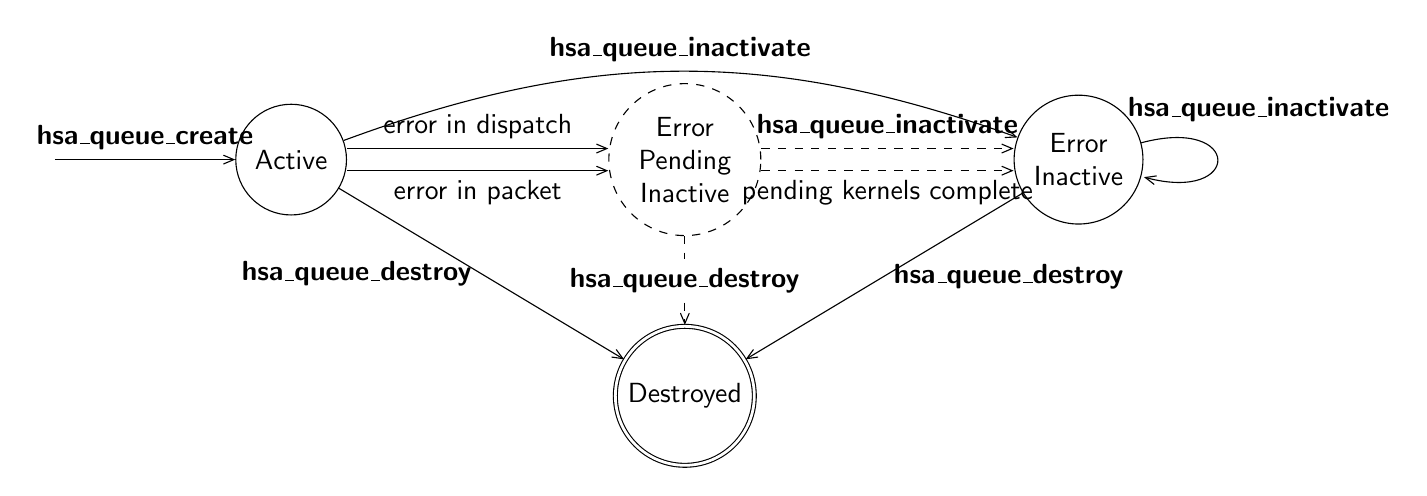
\begin{tikzpicture}[auto,on grid,node distance=5cm,state/.style={circle,draw,minimum size=40pt}]
    \node[state]                 (s0) {Active};
    \node[state,dashed,align=center,right=of s0]       (s1) {Error\\Pending\\Inactive};
    \node[state,align=center,right=of s1]       (s2) {Error\\Inactive};
    \node[state,accepting,double distance=1pt,below=3cm of s1]   (s3) {Destroyed};
    \path[->]
        (-3,0) edge node {\reffun{hsa_queue_create}} (s0)

    ([yshift=-.4em]s0.east) edge  node[below] {error in packet} ([yshift=-.4em]s1.west)
    ([yshift=+.4em]s0.east) edge node[above] {error in dispatch} ([yshift=+.4em]s1.west)
    (s0) edge[bend left=20]  node {\reffun{hsa_queue_inactivate}} (s2)
         edge  node[left] {\reffun{hsa_queue_destroy}} (s3)

    ([yshift=-.4em]s1.east) edge[dashed]  node[below] {pending kernels complete} ([yshift=-.4em]s2.west)
    ([yshift=+.4em]s1.east) edge[dashed] node[above] {\reffun{hsa_queue_inactivate}} ([yshift=+.4em]s2.west)
    (s1) edge[dashed]  node[anchor=center,fill=white] {\reffun{hsa_queue_destroy}} (s3)

    (s2) edge  node[right] {\reffun{hsa_queue_destroy}} (s3)
         edge[loop right] node[anchor=east,above,yshift=+1.0em,xshift=+1.5em] {\reffun{hsa_queue_inactivate}} ()
    ;
  \end{tikzpicture}
  \caption{Queue state diagram.}
  \label{fig:queuestate}
\end{figure}


The queue will report packet processing or parsing error, system error,
dependency resolution error, and signaling error (signal destroyed by the time
it needed to be signaled by packet processor).

The queue error reporting infrastructure supports and reports a single error per
queue and attempts to inactivate the queue on the first error it encounters.

\subsection{Example}
TODO



\section{Architected Queuing Language Support}
\label{AQL}\hypertarget{AQL}{}
AQL is a command interface for describing a dispatch or a dependency in a
standard format for the queue packet processor.The HSA API declares structures
for the different types of AQL packets described in~\cite{sar}: always reserved,
invalid, dispatch, agent dispatch and barrier.

\hypertarget{dispatch-packet}{}\subsection{Dispatch packet}
\label{dispatch-packet}

A dispatch packet is used to submit tasks to a HSA component. It can have five
different states: \emph{on queue}, \emph{launch}, \emph{error},
\emph{active} or \emph{complete}. Figure~\ref{fig:packetstate} shows the
different states of a packet and transitions leading to those states.

\begin{figure}[b]
  \centering
  \scriptsize
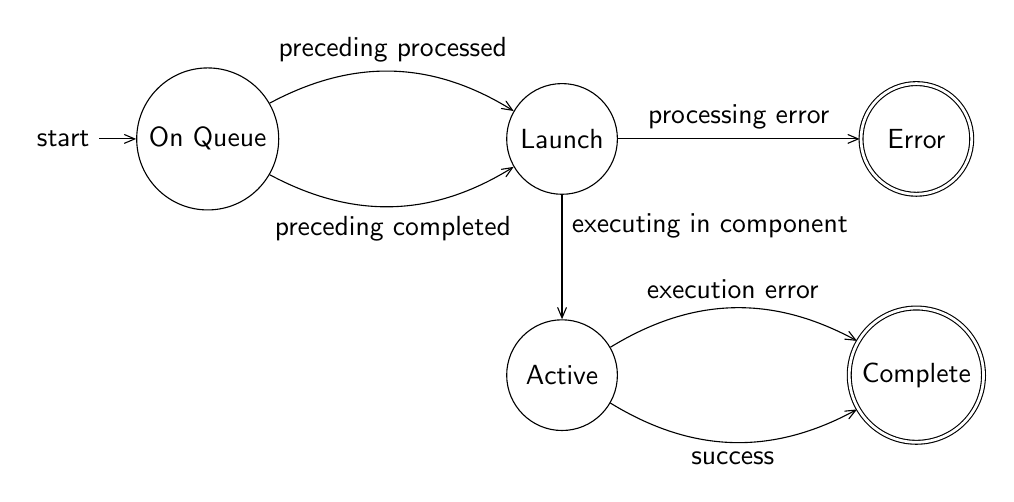
\begin{tikzpicture}
[auto,on grid,node distance=4.5cm,state/.style={circle,draw,minimum size=40pt}]
   \node[state,initial]                 (s0) {On Queue};
   \node[state,right=4.5cm of s0]       (s1) {Launch};
   \node[state,below=3cm of s1]       (s2) {Active};
   \node[state,accepting,double distance=1pt,right=of s1]   (s3) {Error};
   \node[state,accepting,double distance=1pt,right=of s2]   (s4) {Complete};
   \path[->]
     (s0) edge[bend right]  node[below] {preceding completed} (s1)
          edge[bend left] node[above]{preceding processed} (s1)
     (s1) edge  node {processing error} (s3)
          edge  node[near start] {executing in component} (s2)
     (s2) edge[bend right]  node[below] {success} (s4)
          edge[bend left]  node[above] {execution error} (s4)
     ;
\end{tikzpicture}
  \centering
  \caption{Dispatch Packet State Diagram}
  \label{fig:packetstate}
\end{figure}

\begin{description}
\item[On queue] A packet is considered to be in the on queue state once the
  format of the packet is different from
  \refenu{HSA_AQL_PACKET_FORMAT_ALWAYS_RESERVED} and
  \refenu{HSA_AQL_PACKET_FORMAT_INVALID}.

\item[Launch] If this dispatch packet has the barrier bit set, then the
  processing of this packet occurs only after all prior kernels have completed
  execution. Otherwise, the processing starts once the preceding packets have
  completed their launch phase.

\item[Error] the packet processor encountered an error processing this
  packet. This results in a queue error (see Figure~\ref{fig:queuestate}) and
  the packet enters the error state (the completion object is signaled with
  error by the packet processor). The following errors are indicated via an
  error signaled to the completion object: processing parsing error, dependency
  resolution error, system error and premature termination due to queue
  inactivation. When the user invokes the \reffun{hsa_queue_inactivate} API
  or the \reffun{hsa_queue_destroy} API while the packet is in this state, the
  completion object will be signaled with an error.

\item[Active] If the packet processing is successful and the kernel the
  packet represents is either executing or queued for execution, the packet
  enters the active state. From active state, either successful or failed
  execution both take the packet into the completed state. Alternatively, queue
  inactivation can also take the packet out of active state into complete state.
  When the user invokes the \reffun{hsa_queue_inactivate} API or the
  \reffun{hsa_queue_destroy} API while the packet is in this state, the
  completion object will be signaled with an error.

\item[Complete] A packet enters a complete state after its completion
  signal is signaled (either with success or error).
\end{description}

A dispatch packet is considered processed once the packet processor processes it
and makes the queue slot occupied by this packet available. A processed dispatch
packet may endure a period of time where it is awaiting its dispatch on to the
HSA component. Even such packets awaiting execution are still considered as
processed.

\hypertarget{segment-sizes}{}\subsubsection{Segment sizes}
\label{segment-sizes}

If the kernel being dispatched uses private and group segments, the user is
required to specify the sizes of these segments in the dispatch
packet. Manually calculating this information is not feasible and requires
visual inspection of the user program, which itself may have been generated by a
higher-level compiler. Hence the user must rely on the finalizer to get the
corresponding segment sizes. Further details about determining segment sizes are
described in Section~\ref{finalizerchapter}.

Of the other HSA segments, the kernarg segment is also a part of the dispatch
packet, but as a pointer. This is because the kernarg segment carries the
arguments required to execute the kernel being dispatched and must be setup by
the user (the layout of this segment is language/finalization specific and
associated with the code object generated by finalization) prior to writing the
AQL packet to the queue (unlike the group and private segments, whose lifespan
spans only the active state of the dispatch packet). 
\hypertarget{agent-packet}{}\subsection{Agent Dispatch packet}
\label{agent-packet}

Agent Dispatch AQL packets can be used to do dispatches on the agent queue. The
HSA Queue API allows for creation of either agent queues or component queues in
the core API (vendor-specific extensions may support queues that allow both
agent and component dispatches, but it is not a core feature).

\hypertarget{barrier-packet}{}\subsection{Barrier packet}
\label{barrier-packet}

The barrier packet allows the user to specify up to five dependencies as
\reftyp{hsa_signal_t} objects and requires the packet processor to resolve them
before proceeding. The barrier packet is a blocking packet, in that the
processing of the barrier packet completes the packet and its completion object
is signaled. This is unlike a dispatch packet whose completion may occur at some
future time after the packet has finished processing.

If any of the dependent signals have been signaled with a negative value, the
barrier packet is complete, and will indicate failure in its completion
signal. The \reffld{completion_signal} will be signaled with the error value as
discussed in Section~\ref{signals}. If the queue is not already in an error
state (e.g. the job generating the error was processed in a different queue)
then the packet processor should consider the error code on the dependent signal
to indicate an error in the queue itself and subsequently signal the
\reffld{error_signal} in the queue. When all of the dependent signals have been
signaled with the value 0, the \reffld{completion_signal} will be signaled with
the value 0 to indicate a successful completion.

The barrier packet also has a \reffld{barrier} bit that indicates that this
packet may only be processed when all previous packets have been marked as
completed.

The barrier packet can be in one of the following states: \emph{on queue},
\emph{launch}, \emph{completed, error} or \emph{completed,
  success}. Figure~\ref{fig:barrierpacketstate} shows the state transition
diagram.
\begin{figure}
  \centering
  \scriptsize
  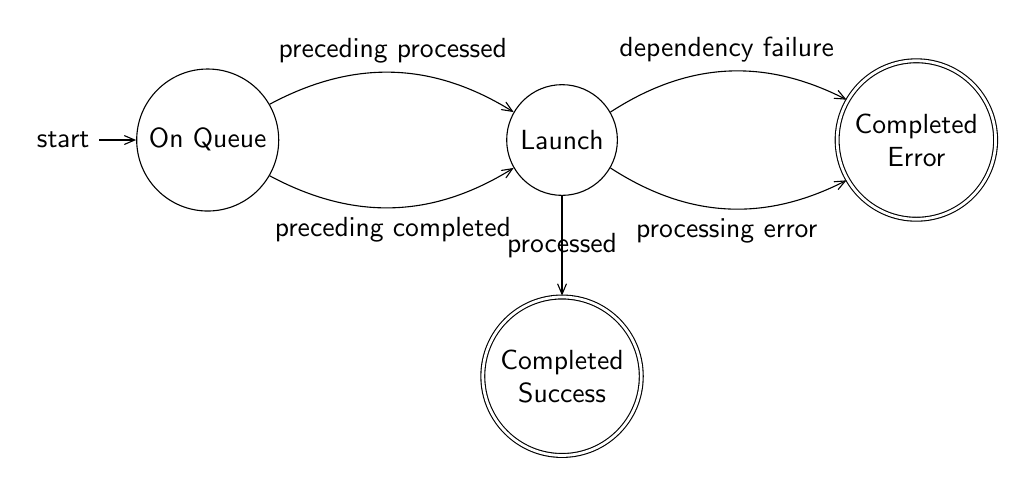
\begin{tikzpicture}[auto,on grid,node distance=4.5cm,state/.style={circle,draw,minimum size=40pt}]
    \node[state,initial]                 (s0) {On Queue};
    \node[state,right=4.5cm of s0]       (s1) {Launch};
    \node[state,accepting,double distance=1pt,align=center,right=of s1]   (s2) {Completed \\Error};
    \node[state,accepting,double distance=1pt,align=center,below=3cm of s1]   (s3) {Completed \\Success};
    \path[->]
    (s0) edge[bend right]  node[below] {preceding completed} (s1)
         edge[bend left] node[above]{preceding processed} (s1)
    (s1) edge[bend right]  node[below] {processing error} (s2)
         edge[bend left] node[above]{dependency failure} (s2)
         edge node[anchor=center] {processed} (s3)
    ;
  \end{tikzpicture}
    \caption{Barrier Packet State Diagram}
  \label{fig:barrierpacketstate}
\end{figure}

\begin{description}
\item[On queue] A packet is considered to be in the on queue state once
  the format of the packet is changed from invalid (a value of 0) to a value of
  1 or 2 or 3. Any other value for format puts the packet and the queue in error
  state.
\item[Launch] If this barrier packet has the barrier bit set, then the
  processing of this packet occurs only after all prior dispatch packets have
  completed execution. Otherwise, once the packets prior to this packet are
  processed, the packet processor begins to process this packet and the packet
  enters the processing state. From the launch state, two states are possible:
  completion, error or completion, success.
\item[Completed with Error] The barrier packet reaches this state from the
  processing state if (a) one of the dependency signals had an error, and (b) if
  the packet was malformed (e.g. bad signal object or invalid usage of reserved
  bits). A barrier packet can also reach this state when the user invokes the
  \reffun{hsa_queue_inactivate} API or the \reffun{hsa_queue_destroy} API while
  the packet is in processing state (the completion object will be appropriately
  signaled with an error).
\item[Completed with Success] The barrier packet had all its dependencies met,
  its completion object has been signaled with a value of 0.
\end{description}

\hypertarget{aql-example}{}\subsection{Example}\label{aql-example}
TODO

\section{Memory}\label{memory}\hypertarget{memory}{}

One of the key features of HSA is its ability to share global pointers between
the host application and code executing on the component. This ability means
that an application can directly pass a pointer to memory allocated on the host
to a kernel function dispatched to a component without an intermediate copy.

\hypertarget{memory-registration}{}\subsection{Registration}\label{memory-registration}

When a buffer will be accessed by a kernel running on a HSA device, programmers
are encouraged to register the corresponding address range beforehand by using
the appropriate HSA core API invocation. While kernels running on HSA devices
can access any valid system memory pointer allocated by means of standard
libraries (for example, malloc in the C language) without resorting to
registration, there might be a performance benefit from registering the buffer
with the HSA core component. When an HSA program no longer needs to access a
registered buffer in a device, the user should deregister that virtual address
range by using the appropriate HSA core API invocation.

\makeatletter{}

\noindent\begin{tcolorbox}[breakable,nobeforeafter,colframe=white,colback=lightgray,left=0mm]
\hyperlink{group--status-1gad755322e7ff95456520e8abdbe90d225}{hsa_status_t} \hypertarget{group--register-1ga13131274af7b6c583b689eaaca3e21f0}{\textbf{hsa_memory_register}}(
\vspace{-3.5mm}\begin{longtable}{@{}p{\textwidth}}
\hspace{1.7em}void * \hsaarg{address},\\
\hspace{1.7em}size_t \hsaarg{size})\end{longtable}

\end{tcolorbox}
Register memory.

\noindent\textbf{Parameters}\\[-6mm]
\noindent\begin{longtable}{@{}>{\hangindent=2em}p{\textwidth}}
\hsaarg{address}\\\hspace{2em}(in) A pointer to the base of the memory region to be registered. If a null pointer is passed, no operation is performed.\\[2mm]
\hsaarg{size}\\\hspace{2em}(in) Requested registration size in bytes. If a size of zero is passed, no operation is performed.
\end{longtable}
\vspace{-5mm}\noindent\textbf{Return Values}\\[-6mm]
\noindent\begin{longtable}{@{}>{\hangindent=2em}p{\linewidth}}
\hyperlink{group--status-1ggad755322e7ff95456520e8abdbe90d225ae382ea0c9c05cce5a60d0317375159cc}{HSA_STATUS_SUCCESS}\\[2mm]
\hyperlink{group--status-1ggad755322e7ff95456520e8abdbe90d225a1a77fcf36d0d140874c4361ab093eff7}{HSA_STATUS_ERROR_OUT_OF_RESOURCES}\\\hspace{2em}If there is a failure in allocating the necessary resources.
\end{longtable}
\vspace{-4mm}\noindent\textbf{Description}\\[1mm]
Registering a system memory region for use with all the available devices This is an optional interface that is solely provided as a performance optimization hint to the underlying implementation so it may prepare for the future use of the memory by the devices. The interface is only beneficial for system memory that will be directly accessed by a device.\\[2mm]
Overlapping registrations are allowed. This is neither detrimental nor beneficial. 


\noindent\begin{tcolorbox}[breakable,nobeforeafter,colframe=white,colback=lightgray,left=0mm]
\hyperlink{group--status-1gad755322e7ff95456520e8abdbe90d225}{hsa_status_t} \hypertarget{group--register-1gab577eaa466b4315f9545e59fdd4b7ec9}{\textbf{hsa_memory_deregister}}(
\vspace{-3.5mm}\begin{longtable}{@{}p{\textwidth}}
\hspace{1.7em}void * \hsaarg{address})\end{longtable}

\end{tcolorbox}
Deregister memory.

\noindent\textbf{Parameters}\\[-6mm]
\noindent\begin{longtable}{@{}>{\hangindent=2em}p{\textwidth}}
\hsaarg{address}\\\hspace{2em}(in) A pointer to the base of the memory region to be deregistered. If a NULL pointer is passed, no operation is performed.
\end{longtable}
\vspace{-5mm}\noindent\textbf{Return Values}\\[-6mm]
\noindent\begin{longtable}{@{}>{\hangindent=2em}p{\linewidth}}
\hyperlink{group--status-1ggad755322e7ff95456520e8abdbe90d225ae382ea0c9c05cce5a60d0317375159cc}{HSA_STATUS_SUCCESS}\\[2mm]
\hyperlink{group--status-1ggad755322e7ff95456520e8abdbe90d225a19fef906a58c2b743e9b375a016582a7}{HSA_STATUS_INFO_NOT_REGISTERED}\\\hspace{2em}If the pointer has not been registered before.
\end{longtable}
\vspace{-4mm}\noindent\textbf{Description}\\[1mm]
Used for deregistering a memory region previously registered.\\[2mm]
Deregistration must be performed using an address that was previously registered. In the event that deregistration is performed on an address that has been used in multiple registrations, the smallest of the registrations is deregistered. 
 

\hypertarget{registration-usage}{}\subsubsection{Example}\label{registration-usage}

A buffer is registered by indicating its starting address and a size. The size
does not need to match that of the original allocation. For example:

\begin{lstlisting}
void* ptr = malloc(16);
status = hsa_memory_register(ptr, 8);
if(status == HSA_STATUS_ERROR_INVALID_ARGUMENT)
  handle_error(status);
\end{lstlisting}

 is a valid program. On the other hand:

\begin{lstlisting}
void* ptr = malloc(16);
status = hsa_memory_register(ptr, 20);
if(status == HSA_STATUS_ERROR_INVALID_ARGUMENT)
  handle_error(status);
\end{lstlisting}

is not a valid program, because we are registering a range that spans several
allocations, or might not be entirely allocated.

Registrations can overlap previously registered intervals. A special case of
overlapped registrations is multiple registration. If the same interval is
registered several times with different sizes, the HSA core component will
select the maximum as the size of all the registrations. Therefore, the
following program:

\begin{lstlisting}
status = hsa_memory_register(ptr, 8);
if(status == HSA_STATUS_ERROR_INVALID_ARGUMENT)
  handle_error(status);
status = hsa_memory_register(ptr, 16);
if(status == HSA_STATUS_ERROR_INVALID_ARGUMENT)
  handle_error(status);
\end{lstlisting}

behaves identically to this program:

\begin{lstlisting}
hsa_memory_register(ptr, 16);
if(status == HSA_STATUS_ERROR_INVALID_ARGUMENT)
  handle_error(status);
hsa_memory_register(ptr, 16);
if(status == HSA_STATUS_ERROR_INVALID_ARGUMENT)
  handle_error(status);
\end{lstlisting}

While the described behavior might seem counter-intuitive, consider the
following scenario: A pointer is registered twice with different sizes s1 and
s2. When the pointer is deregistered, which interval should be deregistered: (p,
s1) or (p, s2)? If all the registrations of the same pointer are considered
identical by the core runtime, that problem is eliminated.

Deregistering a pointer that has not been previously registered results in an
\emph{info} status indicating the same.

The following code snippet revisits the introductory example. The code is almost
identical to the original, except that we register the buffers that will be
accessed from the device after allocating them, and we deregister all that
memory before releasing it. In some platforms, we expect this version to perform
better than the original one.


\hypertarget{globalmemory}{}\subsection{Global  Memory Allocation}\label{globalmemory}

While a HSA component is capable of accessing pageable system memory by
definition, for scenarios where wants memory allocated that has already been
registered (combine the allocation with memory registration), the HSA runtime
provides an interface, \reffun{hsa_memory_allocate} to allocate memory that is
internally registered by the runtime:

\makeatletter{}

\noindent\begin{tcolorbox}[breakable,nobeforeafter,colframe=white,colback=lightgray,left=0mm]
\hyperlink{group--status-1gad755322e7ff95456520e8abdbe90d225}{hsa_status_t} \hypertarget{group--memory--allocate-1gae86946629841221ce6ec2819fbad6e80}{\textbf{hsa_memory_allocate}}(
\vspace{-3.5mm}\begin{longtable}{@{}p{\textwidth}}
\hspace{1.7em}size_t \hsaarg{size_bytes},\\
\hspace{1.7em}void ** \hsaarg{address})\end{longtable}

\end{tcolorbox}
Allocate system memory.

\noindent\textbf{Parameters}\\[-6mm]
\noindent\begin{longtable}{@{}>{\hangindent=2em}p{\textwidth}}
\hsaarg{size_bytes}\\\hspace{2em}(in) Allocation size.\\[2mm]
\hsaarg{address}\\\hspace{2em}(in) Address pointer allocated by the user. Dereferenced and assigned to the pointer to the memory allocated for this request.
\end{longtable}
\vspace{-5mm}\noindent\textbf{Return Values}\\[-6mm]
\noindent\begin{longtable}{@{}>{\hangindent=2em}p{\linewidth}}
\hyperlink{group--status-1ggad755322e7ff95456520e8abdbe90d225ae382ea0c9c05cce5a60d0317375159cc}{HSA_STATUS_SUCCESS}\\[2mm]
\hyperlink{group--status-1ggad755322e7ff95456520e8abdbe90d225a1a77fcf36d0d140874c4361ab093eff7}{HSA_STATUS_ERROR_OUT_OF_RESOURCES}\\\hspace{2em}If there is a failure in allocation. This error may also occur when the core runtime library needs to spawn threads or create internal OS-specific events.\\[2mm]
\hyperlink{group--status-1ggad755322e7ff95456520e8abdbe90d225ac7d3651f75107d2a6a8ba3b25683c030}{HSA_STATUS_ERROR_INVALID_ARGUMENT}\\\hspace{2em}If the passed address is NULL.
\end{longtable}
\vspace{-4mm}\noindent\textbf{Description}\\[1mm]
The returned buffer is already registered. Allocation of size 0 is allowed and returns a NULL pointer. 
 

\hypertarget{kernarg}{}\subsection{Kernarg Memory}\label{kernargmem}

The kernarg memory that AQL packet points to (see Section~\ref{AQL}) holds
information about any arguments required to execute AQL dispatch on a HSA
component. While any system memory may be used for kernarg memory,
implementation/platform specific optimizations are possible if HSA core runtime
provided API are utilized for allocating and copying to the allocated kernarg
memory. To facilitate such optimizations, HSA core runtime defines the following
API:

\makeatletter{}

\noindent\begin{tcolorbox}[breakable,nobeforeafter,colframe=white,colback=lightgray,left=0mm]
\hyperlink{group--status-1gad755322e7ff95456520e8abdbe90d225}{hsa_status_t} \hypertarget{group--kernargmem-1ga9bcec6a182d021007b4c5c2b6b0467fc}{\textbf{hsa_memory_allocate_kernarg}}(
\vspace{-3.5mm}\begin{longtable}{@{}p{\textwidth}}
\hspace{1.7em}const \hyperlink{group--topology-1gab8db3fb886332a24acac08ec361e1d86}{hsa_agent_t} * \hsaarg{component},\\
\hspace{1.7em}size_t \hsaarg{size},\\
\hspace{1.7em}void ** \hsaarg{address})\end{longtable}

\end{tcolorbox}
Allocate kernarg memory.

\noindent\textbf{Parameters}\\[-6mm]
\noindent\begin{longtable}{@{}>{\hangindent=2em}p{\textwidth}}
\hsaarg{component}\\\hspace{2em}(in) A valid pointer to the component for which the specified amount of kernarg memory is to be allocated.\\[2mm]
\hsaarg{size}\\\hspace{2em}(in) Requested allocation size in bytes. If size is 0, NULL is returned.\\[2mm]
\hsaarg{address}\\\hspace{2em}(out) A valid pointer to the location of where to return the pointer to the base of the allocated region of memory.
\end{longtable}
\vspace{-5mm}\noindent\textbf{Return Values}\\[-6mm]
\noindent\begin{longtable}{@{}>{\hangindent=2em}p{\linewidth}}
\hyperlink{group--status-1ggad755322e7ff95456520e8abdbe90d225ae382ea0c9c05cce5a60d0317375159cc}{HSA_STATUS_SUCCESS}\\[2mm]
\hyperlink{group--status-1ggad755322e7ff95456520e8abdbe90d225ac7d3651f75107d2a6a8ba3b25683c030}{HSA_STATUS_ERROR_INVALID_ARGUMENT}\\\hspace{2em}If the passed address is NULL.
\end{longtable}
 


\noindent\begin{tcolorbox}[breakable,nobeforeafter,colframe=white,colback=lightgray,left=0mm]
\hyperlink{group--status-1gad755322e7ff95456520e8abdbe90d225}{hsa_status_t} \hypertarget{group--kernargmem-1gaa47857aa28d4a7e1824a8ca68e691e31}{\textbf{hsa_memory_copy_kernarg_to_system}}(
\vspace{-3.5mm}\begin{longtable}{@{}p{\textwidth}}
\hspace{1.7em}void * \hsaarg{dst},\\
\hspace{1.7em}const void * \hsaarg{src},\\
\hspace{1.7em}size_t \hsaarg{size})\end{longtable}

\end{tcolorbox}
Copy between the system and kernarg segments.

\noindent\textbf{Parameters}\\[-6mm]
\noindent\begin{longtable}{@{}>{\hangindent=2em}p{\textwidth}}
\hsaarg{dst}\\\hspace{2em}(out) A valid pointer to the destination array where the content is to be copied.\\[2mm]
\hsaarg{src}\\\hspace{2em}(in) A valid pointer to the source of data to be copied.\\[2mm]
\hsaarg{size}\\\hspace{2em}(in) Number of bytes to copy.
\end{longtable}
\vspace{-5mm}\noindent\textbf{Return Values}\\[-6mm]
\noindent\begin{longtable}{@{}>{\hangindent=2em}p{\linewidth}}
\hyperlink{group--status-1ggad755322e7ff95456520e8abdbe90d225ae382ea0c9c05cce5a60d0317375159cc}{HSA_STATUS_SUCCESS}\\[2mm]
\hyperlink{group--status-1ggad755322e7ff95456520e8abdbe90d225ac7d3651f75107d2a6a8ba3b25683c030}{HSA_STATUS_ERROR_INVALID_ARGUMENT}\\\hspace{2em}If the source or destination pointers are invalid.
\end{longtable}
 


\noindent\begin{tcolorbox}[breakable,nobeforeafter,colframe=white,colback=lightgray,left=0mm]
\hyperlink{group--status-1gad755322e7ff95456520e8abdbe90d225}{hsa_status_t} \hypertarget{group--kernargmem-1gae89ae228189add9fffc3d6c41355056b}{\textbf{hsa_memory_copy_system_to_kernarg}}(
\vspace{-3.5mm}\begin{longtable}{@{}p{\textwidth}}
\hspace{1.7em}void * \hsaarg{dst},\\
\hspace{1.7em}const void * \hsaarg{src},\\
\hspace{1.7em}size_t \hsaarg{size})\end{longtable}

\end{tcolorbox}
Copy between the system and kernarg segments.

\noindent\textbf{Parameters}\\[-6mm]
\noindent\begin{longtable}{@{}>{\hangindent=2em}p{\textwidth}}
\hsaarg{dst}\\\hspace{2em}(out) A valid pointer to the destination array where the content is to be copied.\\[2mm]
\hsaarg{src}\\\hspace{2em}(in) A valid pointer to the source of data to be copied.\\[2mm]
\hsaarg{size}\\\hspace{2em}(in) Number of bytes to copy.
\end{longtable}
\vspace{-5mm}\noindent\textbf{Return Values}\\[-6mm]
\noindent\begin{longtable}{@{}>{\hangindent=2em}p{\linewidth}}
\hyperlink{group--status-1ggad755322e7ff95456520e8abdbe90d225ae382ea0c9c05cce5a60d0317375159cc}{HSA_STATUS_SUCCESS}\\[2mm]
\hyperlink{group--status-1ggad755322e7ff95456520e8abdbe90d225ac7d3651f75107d2a6a8ba3b25683c030}{HSA_STATUS_ERROR_INVALID_ARGUMENT}\\\hspace{2em}If the source or destination pointers are invalid.
\end{longtable}
 
 

\hypertarget{device-memory}{}\subsection{Component Local Memory}
\label{device-memory}

Component local memory is a memory type that is dedicated specifically for a
particular HSA component. This memory could provide higher bandwidth for
component access (than system memory) with the limitation that the host might
not be able to access it directly. HSA runtime provides a host interface to
allocate/deallocate and access component local memory.

\makeatletter{}

\noindent\begin{tcolorbox}[breakable,nobeforeafter,colframe=white,colback=lightgray,left=0mm]
\hyperlink{group--status-1gad755322e7ff95456520e8abdbe90d225}{hsa_status_t} \hypertarget{group--memory--local-1ga40d441131fce376e8c65ae5087bc916a}{\textbf{hsa_memory_allocate_component_local}}(
\vspace{-3.5mm}\begin{longtable}{@{}p{\textwidth}}
\hspace{1.7em}const \hyperlink{group--topology-1gab8db3fb886332a24acac08ec361e1d86}{hsa_agent_t} * \hsaarg{component},\\
\hspace{1.7em}size_t \hsaarg{size},\\
\hspace{1.7em}void ** \hsaarg{address})\end{longtable}

\end{tcolorbox}
Allocate memory on HSA Device.

\noindent\textbf{Parameters}\\[-6mm]
\noindent\begin{longtable}{@{}>{\hangindent=2em}p{\textwidth}}
\hsaarg{component}\\\hspace{2em}(in) A valid pointer to the HSA device for which the specified amount of global memory is to be allocated.\\[2mm]
\hsaarg{size}\\\hspace{2em}(in) Requested allocation size in bytes. If size is 0, NULL is returned.\\[2mm]
\hsaarg{address}\\\hspace{2em}(out) A valid pointer to the location of where to return the pointer to the base of the allocated region of memory.
\end{longtable}
\vspace{-5mm}\noindent\textbf{Return Values}\\[-6mm]
\noindent\begin{longtable}{@{}>{\hangindent=2em}p{\linewidth}}
\hyperlink{group--status-1ggad755322e7ff95456520e8abdbe90d225ae382ea0c9c05cce5a60d0317375159cc}{HSA_STATUS_SUCCESS}\\[2mm]
\hyperlink{group--status-1ggad755322e7ff95456520e8abdbe90d225a1a77fcf36d0d140874c4361ab093eff7}{HSA_STATUS_ERROR_OUT_OF_RESOURCES}\\\hspace{2em}If there is a failure in allocation of an internal structure required by the core runtime library. This error may also occur when the core runtime library needs to spawn threads or create internal OS-specific events.\\[2mm]
\hyperlink{group--status-1ggad755322e7ff95456520e8abdbe90d225ac7d3651f75107d2a6a8ba3b25683c030}{HSA_STATUS_ERROR_INVALID_ARGUMENT}\\\hspace{2em}If the passed component is NULL or invalid, or if the passed pointer is NULL.
\end{longtable}
\vspace{-4mm}\noindent\textbf{Description}\\[1mm]
Allocate global device memory associated with specified device. 


\noindent\begin{tcolorbox}[breakable,nobeforeafter,colframe=white,colback=lightgray,left=0mm]
\hyperlink{group--status-1gad755322e7ff95456520e8abdbe90d225}{hsa_status_t} \hypertarget{group--memory--local-1gab7716a76b328a81dc0657a4b38faa945}{\textbf{hsa_memory_free_component_local}}(
\vspace{-3.5mm}\begin{longtable}{@{}p{\textwidth}}
\hspace{1.7em}void * \hsaarg{address})\end{longtable}

\end{tcolorbox}
Deallocate memory on HSA component.

\noindent\textbf{Parameters}\\[-6mm]
\noindent\begin{longtable}{@{}>{\hangindent=2em}p{\textwidth}}
\hsaarg{address}\\\hspace{2em}(in) A pointer to the address to be deallocated. If the pointer is NULL, no operation is performed.
\end{longtable}
\vspace{-5mm}\noindent\textbf{Return Values}\\[-6mm]
\noindent\begin{longtable}{@{}>{\hangindent=2em}p{\linewidth}}
\hyperlink{group--status-1ggad755322e7ff95456520e8abdbe90d225ae382ea0c9c05cce5a60d0317375159cc}{HSA_STATUS_SUCCESS}
\end{longtable}
\vspace{-4mm}\noindent\textbf{Description}\\[1mm]
Deallocate component memory that was allocated with \hyperlink{group--memory--local-1ga40d441131fce376e8c65ae5087bc916a}{\reffun{hsa_memory_allocate_component_local}}. 


\noindent\begin{tcolorbox}[breakable,nobeforeafter,colframe=white,colback=lightgray,left=0mm]
\hyperlink{group--status-1gad755322e7ff95456520e8abdbe90d225}{hsa_status_t} \hypertarget{group--memory--local-1ga5733ddfc7ac81df2892396e0ada66bad}{\textbf{hsa_memory_copy_component_local_to_system}}(
\vspace{-3.5mm}\begin{longtable}{@{}p{\textwidth}}
\hspace{1.7em}void * \hsaarg{dst},\\
\hspace{1.7em}const void * \hsaarg{src},\\
\hspace{1.7em}size_t \hsaarg{size},\\
\hspace{1.7em}\hyperlink{group--signals-1ga6592c136d70853d855bc11d9efdbf534}{hsa_signal_handle_t} \hsaarg{signal})\end{longtable}

\end{tcolorbox}
Copy between the system and local heaps.

\noindent\textbf{Parameters}\\[-6mm]
\noindent\begin{longtable}{@{}>{\hangindent=2em}p{\textwidth}}
\hsaarg{dst}\\\hspace{2em}(out) A valid pointer to the destination array where the content is to be copied.\\[2mm]
\hsaarg{src}\\\hspace{2em}(in) A valid pointer to the source of data to be copied.\\[2mm]
\hsaarg{size}\\\hspace{2em}(in) Number of bytes to copy.\\[2mm]
\hsaarg{signal}\\\hspace{2em}(in) The signal that will be incremented by the runtime when the copy is complete.
\end{longtable}
\vspace{-5mm}\noindent\textbf{Return Values}\\[-6mm]
\noindent\begin{longtable}{@{}>{\hangindent=2em}p{\linewidth}}
\hyperlink{group--status-1ggad755322e7ff95456520e8abdbe90d225ae382ea0c9c05cce5a60d0317375159cc}{HSA_STATUS_SUCCESS}\\[2mm]
\hyperlink{group--status-1ggad755322e7ff95456520e8abdbe90d225a1a77fcf36d0d140874c4361ab093eff7}{HSA_STATUS_ERROR_OUT_OF_RESOURCES}\\\hspace{2em}If there is a failure in allocation of an internal structure required by the core runtime library. This error may also occur when the core runtime library needs to spawn threads or create internal OS-specific events.\\[2mm]
\hyperlink{group--status-1ggad755322e7ff95456520e8abdbe90d225ac7d3651f75107d2a6a8ba3b25683c030}{HSA_STATUS_ERROR_INVALID_ARGUMENT}\\\hspace{2em}If any argument is invalid.
\end{longtable}
 
 

\hypertarget{device-memory-usage}{}\subsubsection{Example}\label{device-memory-usage}

Component memory is allocated by indicating the size and the HSA device it
corresponds to. For example, the following code allocates 1024 bytes of device
local memory:

\begin{lstlisting}
void* component_ptr = NULL;
hsa_memory_allocate_component_local(1024, component, &component_ptr);
\end{lstlisting}

To access component memory from the host, the user can call
\reffun{hsa_memory_copy_component_local_to_host} in similar fashion as in
memcpy. This interface allows the user to perform component-to-host memory
copy. For example:

\begin{lstlisting}
 const size_t DATA_SIZE = 1024;
 void* src_ptr = malloc(DATA_SIZE);
 void* dest_ptr = NULL;
 hsa_memory_allocate_component_local(DATA_SIZE, device, &dest_ptr);
 hsa_memory_copy_component_local_to_system(dest_ptr, src_ptr, DATA_SIZE);
\end{lstlisting}

copies 1024 bytes from system to component local memory.

The user should not register or deregister component local memory.









\hypertarget{agent}{}\section{Agent Dispatch Support}\label{agent}

The core runtime supports agent dispatches from an HSA component/Agent. The
runtime defines a default service queue for every user mode queue created by the
user. This default service queue is available to the HSAIL programs and the user
applications may submit agent dispatch packets to the service queue or any user
mode queue. The service queue shares the same structure as the regular HSA
queue. The default service queues are monitored by the
runtime. \makeatletter{}

\noindent\begin{tcolorbox}[breakable,nobeforeafter,colframe=white,colback=lightgray,left=0mm]
\hyperlink{group--status-1gad755322e7ff95456520e8abdbe90d225}{hsa_status_t} \hypertarget{group--agent--dispatch-1ga94c80361fff301b13512caa5269710e5}{\textbf{hsa_register_agent_dispatch_callback}}(
\vspace{-3.5mm}\begin{longtable}{@{}p{\textwidth}}
\hspace{1.7em}\hyperlink{group--queue-1gacbb2835331f18aee30ee441f07b3fc5a}{hsa_queue_t} * \hsaarg{agent_dispatch_queue},\\
\hspace{1.7em}void(*)(uint64_t a0, uint64_t a1, uint64_t a2, uint64_t a3, uint64_t retaddr) \hsaarg{agent_dispatch_callback},\\
\hspace{1.7em}\hyperlink{group--context-1ga0296b674c03f1a65fa8ef91e2f0ad44d}{hsa_runtime_context_t} * \hsaarg{context})\end{longtable}

\end{tcolorbox}
Agent dispatch runtime function registration.

\noindent\textbf{Parameters}\\[-6mm]
\noindent\begin{longtable}{@{}>{\hangindent=2em}p{\textwidth}}
\hsaarg{agent_dispatch_queue}\\\hspace{2em}Agent dispatch queue.\\[2mm]
\hsaarg{agent_dispatch_callback}\\\hspace{2em}(in) Callback that the user is registering, the callback is called with five 64 bit args as a parameter.\\[2mm]
\hsaarg{context}\\\hspace{2em}Context.
\end{longtable}
\vspace{-5mm}\noindent\textbf{Return Values}\\[-6mm]
\noindent\begin{longtable}{@{}>{\hangindent=2em}p{\linewidth}}
\hyperlink{group--status-1ggad755322e7ff95456520e8abdbe90d225ae382ea0c9c05cce5a60d0317375159cc}{HSA_STATUS_SUCCESS}
\end{longtable}
 
 


\hypertarget{extensions}{}\section{Extensions to the Core Runtime
  API}\label{extensions}

When an implementor of the core runtime specification is not supporting any of
the extension API, they will return
\refenu{HSA_STATUS_ERROR_EXTENSION_UNSUPPORTED} as a return status for that API.

Individual vendors may define vendor extensions to HSA core runtime, or multiple
vendors may collaborate to define an extension. The difference is in the naming
scheme used for the symbols (defines, structures, functions, etc.) associated
with the function:

\begin{itemize}
\item Symbols for single-vendor extensions that are defined in the global
  namespace must use the following naming convention:
  \begin{itemize}
  \item \emph{hsa_svext_\textless COMPANY_NAME \textgreater_}. For example,
    a company ``ACME'' defining a single-vendor extension would use the prefix
    \emph{hsa_ext_acme_}. Company names must be registered with the HSA
    Foundation, must be unique, and may be abbreviated to improve the
    readability of the symbols.
  \end{itemize}
\item Symbols for multi-vendor extensions that are defined in the global
  namespace must use the following naming convention:
  \begin{itemize}
  \item \emph{hsa_ext_} For example, if another company embraces extension in
    the example above from Company ``ACME'', the resulting symbols would use the
    prefix \emph{hsa_mvext_}.
  \end{itemize}
\end{itemize}

Any constant definitions in the extension (\#define/enumerations) use the same
naming convention, except using all capital letters. So, using the single-vendor
extension example from above, the associated defines and enumerations would have
the prefix \refenu{HSA_EXT_ACME_}.

The symbols for all vendor extensions (both single-vendor and multi-vendor) are
captured in the file {\bf hsa/vendor_extensions.h}. This file is maintained by
the HSA Foundation. This file includes the enumeration
\reftyp{hsa_vendor_extension_t} which defines a unique code for each vendor
extension and multi-vendor extension. Vendors can reserve enumeration encodings
through the HSA Foundation. Multi-vendor enumerations begin at the value of
1000000. For example, using the examples above, the
\reftyp{hsa_vendor_extension_t} enumeration might be:

\makeatletter{}

\noindent\begin{tcolorbox}[nobeforeafter,arc=0mm,colframe=white,colback=lightgray,left=0mm]
enum \hypertarget{group--vendor--ext-1gaa8dfc9ba0911c03af38071bd3ae0df00}{\textbf{hsa_vendor_extension_t}}
\end{tcolorbox}
Vendor enumeration example.

\noindent\textbf{Values}\\[-5mm]
\begin{longtable}{@{\hspace{2em}}p{\linewidth-2em}}
\hspace{-2em}\hypertarget{group--vendor--ext-1ggaa8dfc9ba0911c03af38071bd3ae0df00a11513e66f5d7fce1a689cdccf8b9f08e}{\refenu{HSA_SVEXT_START}} = 0\\Start of the single vendor extension range.\\[2mm]
\hspace{-2em}\hypertarget{group--vendor--ext-1ggaa8dfc9ba0911c03af38071bd3ae0df00a631ef9884d6dea589e64b6097ca2861a}{\refenu{HSA_SVEXT_ACME_FOO}} = 1\\Company ACME, starts with FOO symbol.\\[2mm]
\hspace{-2em}\hypertarget{group--vendor--ext-1ggaa8dfc9ba0911c03af38071bd3ae0df00af26e003c772ddadf93f47c6125b93ce3}{\refenu{HSA_SVEXT_ACME_ANOTHER_EXT}} = 2\\Company ACME has another_ext symbol.\\[2mm]
\hspace{-2em}\hypertarget{group--vendor--ext-1ggaa8dfc9ba0911c03af38071bd3ae0df00ad24a153c1b1325d152a9a77f4119195f}{\refenu{HSA_MVEXT_START}} = 1000000\\Multi vendor extension starts at 1000000.\\[2mm]
\hspace{-2em}\hypertarget{group--vendor--ext-1ggaa8dfc9ba0911c03af38071bd3ae0df00a00c0f61a4088e94417a9bb2d1afa99d8}{\refenu{HSA_MVEXT_FOO}} = 1000001\\Multivendor extension has a symbol foo.
\end{longtable} 

HSA defines the following query function for vendor extensions:

\makeatletter{}

\noindent\begin{tcolorbox}[breakable,nobeforeafter,colframe=white,colback=lightgray,left=0mm]
\hyperlink{group--status-1gad755322e7ff95456520e8abdbe90d225}{hsa_status_t} \hypertarget{group--query--vendorextension-1gaa21c65dd40f66583e3b17ead871192a6}{\textbf{hsa_vendor_extension_query}}(
\vspace{-3.5mm}\begin{longtable}{@{}p{\textwidth}}
\hspace{1.7em}\hyperlink{group--vendor--ext-1gaa8dfc9ba0911c03af38071bd3ae0df00}{hsa_vendor_extension_t} \hsaarg{extension},\\
\hspace{1.7em}void * \hsaarg{extension_structure})\end{longtable}

\end{tcolorbox}
Query vendor extensions.

\noindent\textbf{Parameters}\\[-6mm]
\noindent\begin{longtable}{@{}>{\hangindent=2em}p{\textwidth}}
\hsaarg{extension}\\\hspace{2em}(in) The vendor extension that is being queried.\\[2mm]
\hsaarg{extension_structure}\\\hspace{2em}(out) Extension structure.
\end{longtable}
\vspace{-5mm}\noindent\textbf{Return Values}\\[-6mm]
\noindent\begin{longtable}{@{}>{\hangindent=2em}p{\linewidth}}
\hyperlink{group--status-1ggad755322e7ff95456520e8abdbe90d225ae382ea0c9c05cce5a60d0317375159cc}{HSA_STATUS_SUCCESS}\\[2mm]
\hyperlink{group--status-1ggad755322e7ff95456520e8abdbe90d225a8f5e5cdc8c12b4263d8b81025d46ffa6}{HSA_STATUS_ERROR_EXTENSION_UNSUPPORTED}\\\hspace{2em}If the extension is not supported.
\end{longtable}
\vspace{-4mm}\noindent\textbf{Description}\\[1mm]
If successful, the extension information is written with extension-specific information such as version information, function pointers, and data values. If the extension is not supported, the extension information is not modified and a error code is returned. 
 

\subsection{Example}
An example that shows a hypothetical single-vendor extension ``Foo'' registered
by company ``ACME''. The example includes four defines and two API functions.
Note the use of the structure \reftyp{hsa_svext_acme_foo_t} and how this
interacts with the \reffun{hsa_vendor_query_extension} API call.

\lstinputlisting{example/extension.c}











\chapter{HSA Extensions Programming Guide}

\section{HSAIL Finalization and Linking}
\label{finalizerchapter} \hypertarget{finalizerchapter}{}

The following subsections have to be updated according to the API definitions
introduced in version 0.180 of the specification.


\hypertarget{finalizer}{}\subsection{HSAIL Finalization}\label{finalizer}

\hypertarget{linking}{}\subsection{HSAIL Linking}\label{linking}





\subsubsection{BRIG and .directive Section}














\subsubsection{Code Objects}\label{finalize:codeobject}














\subsubsection{Finalize BRIG API}







\subsubsection{Freeing The Compilation Unit Code/Debug Object}



\subsubsection{Serializing and Deserializing a Compilation Unit}



\hypertarget{groupmem}{}\subsection{Group Memory
  Usage}\label{groupmem}
















\section{Images and Samplers}
\label{images} \hypertarget{images}{}

Images in HSA are accessed by an image handle \reftyp{hsa_image_handle_t}. The
image handle references the image data in memory and records information about
resource layout and other properties. HSA decouples the storage of the image
data and the description of how the device interprets that data. This allows the
developer to control the location of the image data storage and manage memory
more efficiently.

The HSA image format is specified using a format descriptor
(\reftyp{hsa_image_format_t}) that contains information about the image channel
type and the channel order. The image channel type describes how the data is to
be interpreted along with the bit size, and image channel order describes the
number and the order. Not all image channel types and channel order combinations
are valid on a HSA agent. All HSA agents have to support a required minimum set
of image formats (see HSA Programmer's Reference Manual). An application can
query image format capabilities using \reffun{hsa_image_get_format_capability}.

An implementation-independent image format descriptor
(\reftyp{hsa_image_descriptor_t}) is composed of geometry along with the
image format. The image descriptor is used to inquire the runtime for the HSA
component-specific image data size and alignment details by calling
\reffun{hsa_image_get_info} for the purpose of determining the
implementation's storage requirements.

The memory requirements (\reftyp{hsa_image_info_t}) include the size of the
memory needed as well as any alignment constraints. An application can either
allocate new memory for the image data, or sub-allocate a memory block from an
existing memory if the memory size allows. Before the image data is used, a HSA
agent-specific image handle must be created using it and if necessary, cleared
and prepared according to the intended use.

A HSA agent-specific image handle (\reftyp{hsa_image_handle_t}) is used by the
HSAIL language for reading or writing using HSAIL \refhsl{rdimage},
\refhsl{ldimage} and \refhsl{stimage}
operations. \reffun{hsa_image_create_handle} creates an image handle from a
implementation-independent image format descriptor and independently allocated
image data that conforms to the requirements provided by
\reffun{hsa_image_get_info}.

It must be noted that while the image data technically accessible from its
pointer in the raw form, the data layout and organization is agent-specific and
should be treated as opaque. The internal implementation of an optimal image
data organization could vary depending on the attributes of the image format
descriptor. As a result, there are no guarantees on the data layout when
accessed from another HSA agent. The only reliable way to import or export image
data from optimally organized images is to copy their data to and from a
linearly organized data layout in memory, as specified by the image's format
attributes.

The HSA Runtime provides interfaces to allow operations on images. Image data
transfer to and from memory with a linear layout can be performed using
\reffun{hsa_image_export} and \reffun{hsa_image_import} respectively. A
portion of an image could be copied to another image using
\reffun{hsa_image_copy}. An image can be cleared using
\reffun{hsa_image_clear}. It is the application's responsibility to ensure
proper synchronization and preparation of images on accesses from other image
operations. See HSA System Architecture spec 2.13 for the HSA Image memory
model.

A HSA agent-specific sampler handle (\reftyp{hsa_sampler_handle_t}) is used by
the HSAIL language to describe how images are processed by the \refhsl{rdimage}
HSAIL operation. \reffun{hsa_sampler_create_handle} creates a sampler handle
from an agent independent sampler descriptor
(\reftyp{hsa_sampler_descriptor_t}).

\section{Component Initiated Dispatches} \label{architected}
\hypertarget{architectedchptr}{}

Due to architected support for a queue and design of AQL, HSA supports
component-initiated dispatch, which is the ability for a kernel to dispatch a
new kernel by writing an AQL packet directly to a user queue. In simple use
cases, the AQL packet can be created on the host and passed as a parameter to
the kernel. This eliminates the need to do dynamic memory allocation on the
component, but has the limitation that the problem fanout must be known at the
time the first kernel is launched (so that the AQL packets can be
preallocated). HSA also supports more advanced use cases where the AQL packet is
dynamically allocated (including the memory space for kernel arguments and
spill/arg/private space) on the component. This usage model obviously requires
dynamic component-side memory allocation, for both host and component memory.

Some requirements to do component-initiated dispatch:
\begin{itemize}
\item Ability to dynamically choose a kernel to dispatch: Let us assume for
  example that there are three kernels (A, B and C). If the host launches A,
  then the user has the choice of launching B or C, or even A in case of
  recursion. So, the user should be able to get the ISA and segment size
  (Hsa\-Aql\-Kernel) from the corresponding BRIG dynamically. \mbox{[}caveat:
  The code sample here does not show how we can do this. It assumes that the
  Hsa\-Aql\-Kernel is being passed as an argument to the parent kernel (A in
  this case)\mbox{]}

\item Ability to dynamically allocate memory from the shader: We need to
  allocate memory for AQL\-Packet, different kernel segments in the AQL\-Packet,
  kernel arguments, and so forth.

\item Ability for a finalizer to identify a default HSA queue to write
  AQL\-Packet: The HSA queue information resides in the runtime layer of the
  stack. This needs to be exchanged with the compiler so it can be stored in the
  global space. This way, when the compiler sees the queue, it knows where to
  pick the HSA queue information to write the AQL-Packet.

\item Ability to notify the completion of all the component-initiated
  dispatches on the host:

\begin{itemize}
\item The beginning of execution of the child kernel may or may not wait for the
  parent kernel's completion. This is determined by the user and could be
  algorithm dependent.
\item If the parent (initiated from host) kernel finishes successfully, it means
  all kernels it initiated also finished successfully.
\item To implement this, we need to track the list of kernels launched from the
  parent. Change the status of parent to complete, only if parent and all its
  child kernels have completed successfully.
\end{itemize}
\end{itemize}

Implementations that support component initiated dispatches will need to support
these requirements. If the implementation supports the stated requirements, the
following actions will allow a component to initiate a dispatch:
\begin{itemize}
\item The queue and \reftyp{hsa_code_object_t} (describing the kernel to
  launch) can be passed as arguments to the parent (the one launched from the
  host) kernel. If the dispatch is to the same queue, it is accessible via an
  HSAIL instruction.
\item If not, get the Hsa\-Aql\-Kernel from the BRIG for the kernel that is
  chosen to be dynamically dispatched.
\item When new work is to be created, the HSAIL code would:
\begin{itemize}
\item Use the kernel dynamic memory allocator to allocate a new AQL\-Packet.
\item Use inline HSAIL to replicate the functionality of the
  Hsa\-Init\-AQL\-Packet function. We could perhaps provide an HSAIL library to
  implement this functionality. Recall this function:
\begin{itemize}
\item Copies some fields from the Hsa\-Aql\-Kernel structure (for example, the
  kernel ISA) to the AQL\-Packet
\item Uses a host allocator to allocate memory for the kernel arguments
\item Uses a component allocator to allocate memory for spill, private, and arg
  segments
\end{itemize}
\end{itemize}
\item The HSAIL knows the signature of the called function and can fill in the
  AQL packet with regular HSAIL global store instructions.
\item The HSA queue is architected, so the HSAIL can use memory store
  instructions to dispatch the kernel for dispatch. Depending how the user
  queues are configured, atomic accesses might be necessary to handle contention
  with other writers. Note that, if the queue information is not passed in as an
  argument, the default queue can be chosen by the finalizer as it was exchanged
  earlier from the runtime layer.
\item We also need to handle deallocation of the kernel arguments and
  spill/private/arg space after the kernel completes.
\item On the host, check if the parent has finished. If the parent has finished
  successfully, then it means that all the child kernels have finished
  successfully too. If the parent or any of the child kernels failed, an error
  code will be returned.
\end{itemize}

\begin{appendices}

\chapter{HSA API Reference}

\section{Common data structures}
\makeatletter{}

\noindent\begin{tcolorbox}[nobeforeafter,arc=0mm,colframe=white,colback=lightgray,left=0mm]
typedef uint8_t  \hypertarget{group--RuntimeCommon-1ga143c7c845aca213614c1d79b65c35a0c}{\textbf{hsa_powertwo8_t}}
\end{tcolorbox}
Value expressed as a power of two.
\\

\noindent\begin{tcolorbox}[nobeforeafter,arc=0mm,colframe=white,colback=lightgray,left=0mm]
enum \hypertarget{group--RuntimeCommon-1ga45e8c4edc00ad0dc2c9e6e14e8610977}{\textbf{hsa_powertwo_t}}
\end{tcolorbox}
Power of two between 1 and 256.

\noindent\textbf{Values}\\[-5mm]
\begin{longtable}{@{\hspace{2em}}p{\linewidth-2em}}
\hspace{-2em}\hypertarget{group--RuntimeCommon-1gga45e8c4edc00ad0dc2c9e6e14e8610977a13bfa83a83c0f555efe4bbcca6b9cddf}{\refenu{HSA_POWERTWO_1}} = 0\\[2mm]
\hspace{-2em}\hypertarget{group--RuntimeCommon-1gga45e8c4edc00ad0dc2c9e6e14e8610977a465003dadda71ae8589097dd03202daf}{\refenu{HSA_POWERTWO_2}} = 1\\[2mm]
\hspace{-2em}\hypertarget{group--RuntimeCommon-1gga45e8c4edc00ad0dc2c9e6e14e8610977a04e128660c6aee9bd09b8be8683a4df9}{\refenu{HSA_POWERTWO_4}} = 2\\[2mm]
\hspace{-2em}\hypertarget{group--RuntimeCommon-1gga45e8c4edc00ad0dc2c9e6e14e8610977a6b602015c0db012f426e22c0354fbd05}{\refenu{HSA_POWERTWO_8}} = 3\\[2mm]
\hspace{-2em}\hypertarget{group--RuntimeCommon-1gga45e8c4edc00ad0dc2c9e6e14e8610977abc59007bbaea149704bb50a1aa70b7aa}{\refenu{HSA_POWERTWO_16}} = 4\\[2mm]
\hspace{-2em}\hypertarget{group--RuntimeCommon-1gga45e8c4edc00ad0dc2c9e6e14e8610977af13ebd4aecb93fd78bee555d26ed62a7}{\refenu{HSA_POWERTWO_32}} = 5\\[2mm]
\hspace{-2em}\hypertarget{group--RuntimeCommon-1gga45e8c4edc00ad0dc2c9e6e14e8610977a93252b7ad8bdcbec33390212e8897bd5}{\refenu{HSA_POWERTWO_64}} = 6\\[2mm]
\hspace{-2em}\hypertarget{group--RuntimeCommon-1gga45e8c4edc00ad0dc2c9e6e14e8610977ae78a1c50ad98ae134e34186acd52174e}{\refenu{HSA_POWERTWO_128}} = 7\\[2mm]
\hspace{-2em}\hypertarget{group--RuntimeCommon-1gga45e8c4edc00ad0dc2c9e6e14e8610977ae774bb9d85b5f7f9968ab76e50c23a6b}{\refenu{HSA_POWERTWO_256}} = 8
\end{longtable}

\noindent\begin{tcolorbox}[breakable,nobeforeafter,arc=0mm,colframe=white,colback=lightgray,left=0mm]
typedef struct  hsa_dim3_s \{
\vspace{-3.5mm}\begin{longtable}{@{}p{\textwidth}}
\hspace{1.7em}uint32_t \reffld{x};\\
\hspace{1.7em}uint32_t \reffld{y};\\
\hspace{1.7em}uint32_t \reffld{z};\\
\}  \hypertarget{group--RuntimeCommon-1ga6f7883588491965c45382cd996351aa2}{\textbf{hsa_dim3_t}}
\end{longtable}

\end{tcolorbox}
Three-dimensional coordinate.

\noindent\textbf{Data Fields}\\[-6mm]
\begin{longtable}{@{}>{\hangindent=2em}p{\textwidth}}
\reffld{x}\\\hspace{2em}X dimension.\\[2mm]
\reffld{y}\\\hspace{2em}Y dimension.\\[2mm]
\reffld{z}\\\hspace{2em}Z dimension
\end{longtable}



\noindent\begin{tcolorbox}[breakable,nobeforeafter,arc=0mm,colframe=white,colback=lightgray,left=0mm]
typedef struct  hsa_runtime_caller_s \{
\vspace{-3.5mm}\begin{longtable}{@{}p{\textwidth}}
\hspace{1.7em}uint64_t \reffld{caller};\\
\}  \hypertarget{group--RuntimeCommon-1ga7d9b1191602415f5dd3893985cc93826}{\textbf{hsa_runtime_caller_t}}
\end{longtable}

\end{tcolorbox}
Opaque pointer which is passed to all runtime functions that use callbacks. It is passed as the first argument to all callbacks made by the function.

\noindent\textbf{Data Fields}\\[-6mm]
\begin{longtable}{@{}>{\hangindent=2em}p{\textwidth}}
\reffld{caller}\\\hspace{2em}Opaque pointer which is passed as the first argument to callback functions invoked by a runtime function.
\end{longtable}



\noindent\begin{tcolorbox}[nobeforeafter,arc=0mm,colframe=white,colback=lightgray,left=0mm]
typedef hsa_status_t(*  \hypertarget{group--RuntimeCommon-1gabd2ff48bd8e2fec466eb5b561e07fec7}{\textbf{hsa_runtime_alloc_data_t}})(hsa_runtime_caller_t caller, size_t byte_size, void **address)
\end{tcolorbox}
Call back function for allocating data.
\\ 

\section{Initialization and Shutdown}
\makeatletter{}

\noindent\begin{tcolorbox}[nobeforeafter,arc=0mm,colframe=white,colback=lightgray,left=0mm]
typedef uint64_t  \hypertarget{group--context-1ga0296b674c03f1a65fa8ef91e2f0ad44d}{\textbf{hsa_runtime_context_t}}
\end{tcolorbox}
Opaque object representing a runtime context.
\\

\noindent\begin{tcolorbox}[breakable,nobeforeafter,colframe=white,colback=lightgray,left=0mm]
\hyperlink{group--status-1gad755322e7ff95456520e8abdbe90d225}{hsa_status_t} \hypertarget{group--context-1gab45607a30ab05c95dfe692115fe1f2a4}{\textbf{hsa_open}}(
\vspace{-3.5mm}\begin{longtable}{@{}p{\textwidth}}
\hspace{1.7em}\hyperlink{group--context-1ga0296b674c03f1a65fa8ef91e2f0ad44d}{hsa_runtime_context_t} ** \hsaarg{context})\end{longtable}

\end{tcolorbox}
Initialize the HSA runtime.

\noindent\textbf{Parameters}\\[-6mm]
\noindent\begin{longtable}{@{}>{\hangindent=2em}p{\textwidth}}
\hsaarg{context}\\\hspace{2em}(out) A valid pointer to a runtime context.
\end{longtable}
\vspace{-5mm}\noindent\textbf{Return Values}\\[-6mm]
\noindent\begin{longtable}{@{}>{\hangindent=2em}p{\linewidth}}
\hyperlink{group--status-1ggad755322e7ff95456520e8abdbe90d225ae382ea0c9c05cce5a60d0317375159cc}{HSA_STATUS_SUCCESS}\\[2mm]
\hyperlink{group--status-1ggad755322e7ff95456520e8abdbe90d225a1a77fcf36d0d140874c4361ab093eff7}{HSA_STATUS_ERROR_OUT_OF_RESOURCES}\\\hspace{2em}If there is a failure in allocation of an internal structure required by the core runtime library. This error may also occur when the core runtime library needs to spawn threads or create internal OS-specific events.\\[2mm]
\hyperlink{group--status-1ggad755322e7ff95456520e8abdbe90d225ac2b1926b00231fd6a7695c1470c43ef6}{HSA_STATUS_ERROR_COMPONENT_INITIALIZATION}\\\hspace{2em}If there is a non-specific failure in initializing one of the components.\\[2mm]
\hyperlink{group--status-1ggad755322e7ff95456520e8abdbe90d225a2ae9f2db427b200c2709bac49f4cabfb}{HSA_STATUS_ERROR_CONTEXT_NULL}\\\hspace{2em}If the context pointer passed by the user is NULL. User is required to pass in a memory backed context pointer.
\end{longtable}
\vspace{-4mm}\noindent\textbf{Description}\\[1mm]
Initializes the HSA runtime if it is not already initialized. It is allowed for applications to invoke this function multiple times. The open call returns a new context for every invocation. Reference counting is a mechanism that allows the runtime to keep a count of the number of different usages of the runtime API within the same application process. This ensures that the runtime stays active until \hyperlink{group--context-1gae008f9f4f2d3939b2ccd1c378b8cc4f0}{\reffun{hsa_close}} is called by the user when the reference count represented by that runtime context is one.\\[2mm]
If the HSA runtime is already initialized, an asynchronous notification is generated by the runtime and \hyperlink{group--status-1ggad755322e7ff95456520e8abdbe90d225ae382ea0c9c05cce5a60d0317375159cc}{HSA_STATUS_SUCCESS} is returned. If the user chooses to capture this asynchronous notification, the user should define a callback and associate it with the context returned by the \hyperlink{group--context-1gab45607a30ab05c95dfe692115fe1f2a4}{\reffun{hsa_open}} call. Each open call increments the reference count before returning success. 


\noindent\begin{tcolorbox}[breakable,nobeforeafter,colframe=white,colback=lightgray,left=0mm]
\hyperlink{group--status-1gad755322e7ff95456520e8abdbe90d225}{hsa_status_t} \hypertarget{group--context-1gae008f9f4f2d3939b2ccd1c378b8cc4f0}{\textbf{hsa_close}}(
\vspace{-3.5mm}\begin{longtable}{@{}p{\textwidth}}
\hspace{1.7em}\hyperlink{group--context-1ga0296b674c03f1a65fa8ef91e2f0ad44d}{hsa_runtime_context_t} * \hsaarg{context})\end{longtable}

\end{tcolorbox}
Close the HSA runtime.

\noindent\textbf{Parameters}\\[-6mm]
\noindent\begin{longtable}{@{}>{\hangindent=2em}p{\textwidth}}
\hsaarg{context}\\\hspace{2em}(in) Context to close.
\end{longtable}
\vspace{-5mm}\noindent\textbf{Return Values}\\[-6mm]
\noindent\begin{longtable}{@{}>{\hangindent=2em}p{\linewidth}}
\hyperlink{group--status-1ggad755322e7ff95456520e8abdbe90d225ae382ea0c9c05cce5a60d0317375159cc}{HSA_STATUS_SUCCESS}\\[2mm]
\hyperlink{group--status-1ggad755322e7ff95456520e8abdbe90d225a34ea59ade5bfce95eee935238a99f5b5}{HSA_STATUS_ERROR_NOT_INITIALIZED}\\\hspace{2em}If invoked before the runtime was initialized, or after it has already been successfully closed.\\[2mm]
\hyperlink{group--status-1ggad755322e7ff95456520e8abdbe90d225a6406af88203fcbec4179fbb71cc66b65}{HSA_STATUS_ERROR_RESOURCE_FREE}\\\hspace{2em}If some of the resources consumed during initialization by the runtime could not be freed.
\end{longtable}
\vspace{-4mm}\noindent\textbf{Description}\\[1mm]
Decreases the context reference count for every invocation. Once the reference count is zero, it proceeds to relinquish any resources allocated for the runtime and closes the runtime instance. It is possible in a multi-threaded scenario that one thread is doing a close while the other is trying to acquire the runtime context or do an open. The core runtime specification defines that an acquire with an input context that represents a closed runtime instance will fail. However, \hyperlink{group--context-1gab45607a30ab05c95dfe692115fe1f2a4}{\reffun{hsa_open}} can be called to create a new instance of the runtime after it is closed.\\[2mm]
An invocation when the reference count is not one it is considered successful in that \hyperlink{group--status-1ggad755322e7ff95456520e8abdbe90d225ae382ea0c9c05cce5a60d0317375159cc}{HSA_STATUS_SUCCESS} is returned with status \hyperlink{group--status-1ggad755322e7ff95456520e8abdbe90d225ae2924e022da18c1062e3b418a5bab43c}{HSA_STATUS_CLOSE_CONTEXT_ACTIVE}, is generated by the runtime on the context that is still active before the API returns. 


\noindent\begin{tcolorbox}[breakable,nobeforeafter,colframe=white,colback=lightgray,left=0mm]
\hyperlink{group--status-1gad755322e7ff95456520e8abdbe90d225}{hsa_status_t} \hypertarget{group--context-1gac10422c957e78aa183b830495c20cd25}{\textbf{hsa_context_acquire}}(
\vspace{-3.5mm}\begin{longtable}{@{}p{\textwidth}}
\hspace{1.7em}\hyperlink{group--context-1ga0296b674c03f1a65fa8ef91e2f0ad44d}{hsa_runtime_context_t} * \hsaarg{input_context})\end{longtable}

\end{tcolorbox}
Increment reference count of a context, if it is not currently zero.

\noindent\textbf{Parameters}\\[-6mm]
\noindent\begin{longtable}{@{}>{\hangindent=2em}p{\textwidth}}
\hsaarg{input_context}\\\hspace{2em}(in) The context that the user is explicitly reference counting.
\end{longtable}
\vspace{-5mm}\noindent\textbf{Return Values}\\[-6mm]
\noindent\begin{longtable}{@{}>{\hangindent=2em}p{\linewidth}}
\hyperlink{group--status-1ggad755322e7ff95456520e8abdbe90d225ae382ea0c9c05cce5a60d0317375159cc}{HSA_STATUS_SUCCESS}\\[2mm]
\hyperlink{group--status-1ggad755322e7ff95456520e8abdbe90d225a34ea59ade5bfce95eee935238a99f5b5}{HSA_STATUS_ERROR_NOT_INITIALIZED}\\\hspace{2em}If invoked before the runtime was initialized or after it has been closed.\\[2mm]
\hyperlink{group--status-1ggad755322e7ff95456520e8abdbe90d225a342227d93a263cefbacb5cde75fa386f}{HSA_STATUS_CONTEXT_LIMIT_REACHED}\\\hspace{2em}If the reference count has reached UINT64_MAX.
\end{longtable}
 


\noindent\begin{tcolorbox}[breakable,nobeforeafter,colframe=white,colback=lightgray,left=0mm]
\hyperlink{group--status-1gad755322e7ff95456520e8abdbe90d225}{hsa_status_t} \hypertarget{group--context-1ga9e080a819a1114577ccb53cc7f767470}{\textbf{hsa_context_release}}(
\vspace{-3.5mm}\begin{longtable}{@{}p{\textwidth}}
\hspace{1.7em}\hyperlink{group--context-1ga0296b674c03f1a65fa8ef91e2f0ad44d}{hsa_runtime_context_t} * \hsaarg{input_context})\end{longtable}

\end{tcolorbox}
Decrement reference count of a context.

\noindent\textbf{Parameters}\\[-6mm]
\noindent\begin{longtable}{@{}>{\hangindent=2em}p{\textwidth}}
\hsaarg{input_context}\\\hspace{2em}(in) The context that the user is explicitly reference counting.
\end{longtable}
\vspace{-5mm}\noindent\textbf{Return Values}\\[-6mm]
\noindent\begin{longtable}{@{}>{\hangindent=2em}p{\linewidth}}
\hyperlink{group--status-1ggad755322e7ff95456520e8abdbe90d225ae382ea0c9c05cce5a60d0317375159cc}{HSA_STATUS_SUCCESS}\\[2mm]
\hyperlink{group--status-1ggad755322e7ff95456520e8abdbe90d225a34ea59ade5bfce95eee935238a99f5b5}{HSA_STATUS_ERROR_NOT_INITIALIZED}\\\hspace{2em}If invoked before the runtime was initialized or when the reference count is already zero.
\end{longtable}
 
 

\section{Errors and Notifications}
\makeatletter{}

\noindent\begin{tcolorbox}[nobeforeafter,arc=0mm,colframe=white,colback=lightgray,left=0mm]
enum \hypertarget{group--status-1gad755322e7ff95456520e8abdbe90d225}{\textbf{hsa_status_t}}
\end{tcolorbox}


\noindent\textbf{Values}\\[-5mm]
\begin{longtable}{@{\hspace{2em}}p{\linewidth-2em}}
\hspace{-2em}\hypertarget{group--status-1ggad755322e7ff95456520e8abdbe90d225ae382ea0c9c05cce5a60d0317375159cc}{\refenu{HSA_STATUS_SUCCESS}} = 0\\Indicates success. The API has been successfully executed per its definition.\\[2mm]
\hspace{-2em}\hypertarget{group--status-1ggad755322e7ff95456520e8abdbe90d225a49e95a9eebe62315fa4c80e699b68eeb}{\refenu{HSA_STATUS_FAILURE}} \\Indicates an error occurred, specifics were either not determinable or not encoded in the error list.\\[2mm]
\hspace{-2em}\hypertarget{group--status-1ggad755322e7ff95456520e8abdbe90d225a10496aec7462cb613a5aa589510cacc9}{\refenu{HSA_STATUS_ALREADY_INITIALIZED}} \\Indicates that initialization attempt failed due to prior initialization.\\[2mm]
\hspace{-2em}\hypertarget{group--status-1ggad755322e7ff95456520e8abdbe90d225a96e987aac8207e7a0f92fb8a8d73b91e}{\refenu{HSA_STATUS_INFO_SIGNAL_TIMEOUT}} \\Indicates that signal is timed out.\\[2mm]
\hspace{-2em}\hypertarget{group--status-1ggad755322e7ff95456520e8abdbe90d225ac7d3651f75107d2a6a8ba3b25683c030}{\refenu{HSA_STATUS_ERROR_INVALID_ARGUMENT}} \\TODO.\\[2mm]
\hspace{-2em}\hypertarget{group--status-1ggad755322e7ff95456520e8abdbe90d225a1a77fcf36d0d140874c4361ab093eff7}{\refenu{HSA_STATUS_ERROR_OUT_OF_RESOURCES}} \\The runtime was not able to allocate the necessary resources. This error may also occur when the core runtime library needs to spawn threads or create internal OS-specific events.\\[2mm]
\hspace{-2em}\hypertarget{group--status-1ggad755322e7ff95456520e8abdbe90d225a7bd6aaae8ecaaaea4c0d12e406e13b53}{\refenu{HSA_STATUS_ERROR_INVALID_CONTEXT}} \\TODO.\\[2mm]
\hspace{-2em}\hypertarget{group--status-1ggad755322e7ff95456520e8abdbe90d225ace44d3eaae9507c7dfc6d6d5e886ee1d}{\refenu{HSA_STATUS_ERROR_TOPOLOGY_CHANGE}} \\The topology information is out-of-date because the available HW has changed.\\[2mm]
\hspace{-2em}\hypertarget{group--status-1ggad755322e7ff95456520e8abdbe90d225ad86a1ebe53e881974cd767c77aa598a3}{\refenu{HSA_STATUS_INFO_UNRECOGNIZED_OPTIONS}} \\TODO.\\[2mm]
\hspace{-2em}\hypertarget{group--status-1ggad755322e7ff95456520e8abdbe90d225a456240e6020bd5de7d4533a948a7df03}{\refenu{HSA_STATUS_ERROR_DIRECTIVE_MISMATCH}} \\TODO.\\[2mm]
\hspace{-2em}\hypertarget{group--status-1ggad755322e7ff95456520e8abdbe90d225a6406af88203fcbec4179fbb71cc66b65}{\refenu{HSA_STATUS_ERROR_RESOURCE_FREE}} \\TODO.\\[2mm]
\hspace{-2em}\hypertarget{group--status-1ggad755322e7ff95456520e8abdbe90d225ae2924e022da18c1062e3b418a5bab43c}{\refenu{HSA_STATUS_CLOSE_CONTEXT_ACTIVE}} \\TODO.\\[2mm]
\hspace{-2em}\hypertarget{group--status-1ggad755322e7ff95456520e8abdbe90d225a34ea59ade5bfce95eee935238a99f5b5}{\refenu{HSA_STATUS_ERROR_NOT_INITIALIZED}} \\TODO.\\[2mm]
\hspace{-2em}\hypertarget{group--status-1ggad755322e7ff95456520e8abdbe90d225a342227d93a263cefbacb5cde75fa386f}{\refenu{HSA_STATUS_CONTEXT_LIMIT_REACHED}} \\TODO.\\[2mm]
\hspace{-2em}\hypertarget{group--status-1ggad755322e7ff95456520e8abdbe90d225ac2b1926b00231fd6a7695c1470c43ef6}{\refenu{HSA_STATUS_ERROR_COMPONENT_INITIALIZATION}} \\TODO.\\[2mm]
\hspace{-2em}\hypertarget{group--status-1ggad755322e7ff95456520e8abdbe90d225a2ae9f2db427b200c2709bac49f4cabfb}{\refenu{HSA_STATUS_ERROR_CONTEXT_NULL}} \\TODO.\\[2mm]
\hspace{-2em}\hypertarget{group--status-1ggad755322e7ff95456520e8abdbe90d225ab8041363ce358439720850c37d0fdf0c}{\refenu{HSA_STATUS_ERROR_SIGNAL_NOT_BOUND}} \\TODO.\\[2mm]
\hspace{-2em}\hypertarget{group--status-1ggad755322e7ff95456520e8abdbe90d225a60edf4d82e4703ff750ea38d619fea88}{\refenu{HSA_STATUS_ERROR}} \\TODO.\\[2mm]
\hspace{-2em}\hypertarget{group--status-1ggad755322e7ff95456520e8abdbe90d225a19fef906a58c2b743e9b375a016582a7}{\refenu{HSA_STATUS_INFO_NOT_REGISTERED}} \\TODO.\\[2mm]
\hspace{-2em}\hypertarget{group--status-1ggad755322e7ff95456520e8abdbe90d225a8f5e5cdc8c12b4263d8b81025d46ffa6}{\refenu{HSA_STATUS_ERROR_EXTENSION_UNSUPPORTED}} \\TODO.\\[2mm]
\hspace{-2em}\hypertarget{group--status-1ggad755322e7ff95456520e8abdbe90d225a39a0056af36f595267930575af7889ed}{\refenu{HSA_STATUS_ERROR_IMAGE_FORMAT_UNSUPPORTED}} \\TODO.\\[2mm]
\hspace{-2em}\hypertarget{group--status-1ggad755322e7ff95456520e8abdbe90d225ad74e9bee6d85a6c5c11e8a9843320be3}{\refenu{HSA_STATUS_ERROR_IMAGE_SIZE_UNSUPPORTED}} \\TODO.
\end{longtable}

\noindent\begin{tcolorbox}[breakable,nobeforeafter,arc=0mm,colframe=white,colback=lightgray,left=0mm]
typedef struct  _hsa_notification_info_s \{
\vspace{-3.5mm}\begin{longtable}{@{}p{\textwidth}}
\hspace{1.7em}\hyperlink{group--status-1gad755322e7ff95456520e8abdbe90d225}{hsa_status_t} \reffld{status};\\
\hspace{1.7em}void * \reffld{info};\\
\hspace{1.7em}char * \reffld{string_info};\\
\hspace{1.7em}void * \reffld{user_data};\\
\}  \hypertarget{group--status-1ga46fc2648e5bde0dfc932de4acb246d82}{\textbf{hsa_notification_info_t}}
\end{longtable}

\end{tcolorbox}
Notification information.

\noindent\textbf{Data Fields}\\[-6mm]
\begin{longtable}{@{}>{\hangindent=2em}p{\textwidth}}
\reffld{status}\\\hspace{2em}Notification type.\\[2mm]
\reffld{info}\\\hspace{2em}A pointer to more information, this could be pointing to implementation specific details that could be useful to some tools or to binary data.\\[2mm]
\reffld{string_info}\\\hspace{2em}A string containing further information. ISO/IEC 646 character encoding must be used. The string should be NUL terminated.\\[2mm]
\reffld{user_data}\\\hspace{2em}A pointer to user supplied data.
\end{longtable}



\noindent\begin{tcolorbox}[breakable,nobeforeafter,arc=0mm,colframe=white,colback=lightgray,left=0mm]
typedef struct  _hsa_async_error_info_s \{
\vspace{-3.5mm}\begin{longtable}{@{}p{\textwidth}}
\hspace{1.7em}\hyperlink{group--status-1gad755322e7ff95456520e8abdbe90d225}{hsa_status_t} \reffld{status};\\
\hspace{1.7em}uint32_t \reffld{queue_id};\\
\hspace{1.7em}void * \reffld{info};\\
\hspace{1.7em}char * \reffld{string_info};\\
\hspace{1.7em}void * \reffld{user_data};\\
\hspace{1.7em}uint64_t \reffld{timestamp};\\
\hspace{1.7em}uint64_t \reffld{reserved1};\\
\hspace{1.7em}uint64_t \reffld{reserved2};\\
\hspace{1.7em}uint64_t \reffld{reserved3};\\
\}  \hypertarget{group--status-1ga1e98022fc32cd651dc83c5f871e1a960}{\textbf{hsa_async_error_info_t}}
\end{longtable}

\end{tcolorbox}
TODO.

\noindent\textbf{Data Fields}\\[-6mm]
\begin{longtable}{@{}>{\hangindent=2em}p{\textwidth}}
\reffld{status}\\\hspace{2em}Error type.\\[2mm]
\reffld{queue_id}\\\hspace{2em}The queue that processed the entity that caused the asynchronous error.\\[2mm]
\reffld{info}\\\hspace{2em}A pointer to more information, this could be pointing to implementation specific details that could be useful to some tools or to binary data.\\[2mm]
\reffld{string_info}\\\hspace{2em}A string containing further information. ISO/IEC 646 character encoding must be used. The string should be NUL terminated.\\[2mm]
\reffld{user_data}\\\hspace{2em}A pointer to user supplied data\\[2mm]
\reffld{timestamp}\\\hspace{2em}System timestamp to indicate when the error was discovered, the implementation may chose to always return 0.\\[2mm]
\reffld{reserved1}\\\hspace{2em}Additional info to be interpreted based on \textit{status}.\\[2mm]
\reffld{reserved2}\\\hspace{2em}Additional info to be interpreted based on \textit{status}.\\[2mm]
\reffld{reserved3}\\\hspace{2em}Additional info to be interpreted based on \textit{status}.
\end{longtable}



\noindent\begin{tcolorbox}[breakable,nobeforeafter,colframe=white,colback=lightgray,left=0mm]
\hyperlink{group--status-1gad755322e7ff95456520e8abdbe90d225}{hsa_status_t} \hypertarget{group--status-1ga45cd274e6ebdd03ed401e28cc85c29c5}{\textbf{hsa_notification_callback_register}}(
\vspace{-3.5mm}\begin{longtable}{@{}p{\textwidth}}
\hspace{1.7em}void(*)(const \hyperlink{group--status-1ga46fc2648e5bde0dfc932de4acb246d82}{hsa_notification_info_t} *info) \hsaarg{callback},\\
\hspace{1.7em}void * \hsaarg{user_data},\\
\hspace{1.7em}\hyperlink{group--context-1ga0296b674c03f1a65fa8ef91e2f0ad44d}{hsa_runtime_context_t} * \hsaarg{context})\end{longtable}

\end{tcolorbox}
Register a notification callback.

\noindent\textbf{Parameters}\\[-6mm]
\noindent\begin{longtable}{@{}>{\hangindent=2em}p{\textwidth}}
\hsaarg{callback}\\\hspace{2em}(in) The callback that the user is registering\\[2mm]
\hsaarg{user_data}\\\hspace{2em}(in) The user data to call the callback with. The \textit{user_data} field of the notification information is populated with this value before the callback is invoked.\\[2mm]
\hsaarg{context}\\\hspace{2em}(in) Identifies a particular runtime context that this callback is registered for. When a callback is registered for a particular context, it will only be invoked if the notification is for an action in that context.
\end{longtable}
\vspace{-5mm}\noindent\textbf{Return Values}\\[-6mm]
\noindent\begin{longtable}{@{}>{\hangindent=2em}p{\linewidth}}
\hyperlink{group--status-1ggad755322e7ff95456520e8abdbe90d225ae382ea0c9c05cce5a60d0317375159cc}{HSA_STATUS_SUCCESS}\\[2mm]
\hyperlink{group--status-1ggad755322e7ff95456520e8abdbe90d225a1a77fcf36d0d140874c4361ab093eff7}{HSA_STATUS_ERROR_OUT_OF_RESOURCES}\\[2mm]
\hyperlink{group--status-1ggad755322e7ff95456520e8abdbe90d225ac7d3651f75107d2a6a8ba3b25683c030}{HSA_STATUS_ERROR_INVALID_ARGUMENT}\\\hspace{2em}If \textit{callback} is NULL.\\[2mm]
\hyperlink{group--status-1ggad755322e7ff95456520e8abdbe90d225a7bd6aaae8ecaaaea4c0d12e406e13b53}{HSA_STATUS_ERROR_INVALID_CONTEXT}\\\hspace{2em}If the context is NULL or invalid (e.g. referenced counted to 0).
\end{longtable}
 


\noindent\begin{tcolorbox}[breakable,nobeforeafter,colframe=white,colback=lightgray,left=0mm]
\hyperlink{group--status-1gad755322e7ff95456520e8abdbe90d225}{hsa_status_t} \hypertarget{group--status-1gafd8fb108ce9ca4862ef939c0477e1793}{\textbf{hsa_error_callback_register}}(
\vspace{-3.5mm}\begin{longtable}{@{}p{\textwidth}}
\hspace{1.7em}void(*)(const \hyperlink{group--status-1ga1e98022fc32cd651dc83c5f871e1a960}{hsa_async_error_info_t} *info) \hsaarg{callback},\\
\hspace{1.7em}void * \hsaarg{user_data},\\
\hspace{1.7em}\hyperlink{group--context-1ga0296b674c03f1a65fa8ef91e2f0ad44d}{hsa_runtime_context_t} * \hsaarg{context})\end{longtable}

\end{tcolorbox}
Register an error callback.

\noindent\textbf{Parameters}\\[-6mm]
\noindent\begin{longtable}{@{}>{\hangindent=2em}p{\textwidth}}
\hsaarg{callback}\\\hspace{2em}(in) The callback that the user is registering\\[2mm]
\hsaarg{user_data}\\\hspace{2em}(in) The user data to call the callback with. The \textit{user_data} field of the error information is populated with this value before the callback is invoked.\\[2mm]
\hsaarg{context}\\\hspace{2em}(in) The runtime context that this callback is being registered for.
\end{longtable}
\vspace{-5mm}\noindent\textbf{Return Values}\\[-6mm]
\noindent\begin{longtable}{@{}>{\hangindent=2em}p{\linewidth}}
\hyperlink{group--status-1ggad755322e7ff95456520e8abdbe90d225ae382ea0c9c05cce5a60d0317375159cc}{HSA_STATUS_SUCCESS}\\[2mm]
\hyperlink{group--status-1ggad755322e7ff95456520e8abdbe90d225a1a77fcf36d0d140874c4361ab093eff7}{HSA_STATUS_ERROR_OUT_OF_RESOURCES}\\[2mm]
\hyperlink{group--status-1ggad755322e7ff95456520e8abdbe90d225a7bd6aaae8ecaaaea4c0d12e406e13b53}{HSA_STATUS_ERROR_INVALID_CONTEXT}\\\hspace{2em}If the context is NULL or invalid (e.g. referenced counted to 0).
\end{longtable}
\vspace{-4mm}\noindent\textbf{Description}\\[1mm]
When a callback is registered for a particular context, it will only be invoked if the notification is for an action in that context. For example, if a queue was created for a runtime context \textit{c1} and a callback has been registered only for context \textit{c2}, then any error on the queue, such as a packet processing error, will not trigger any asynchronous error callback. 


\noindent\begin{tcolorbox}[breakable,nobeforeafter,colframe=white,colback=lightgray,left=0mm]
\hyperlink{group--status-1gad755322e7ff95456520e8abdbe90d225}{hsa_status_t} \hypertarget{group--status-1gaf3032aa83b93991d945e572fce1f8fec}{\textbf{hsa_status_query_description}}(
\vspace{-3.5mm}\begin{longtable}{@{}p{\textwidth}}
\hspace{1.7em}\hyperlink{group--status-1gad755322e7ff95456520e8abdbe90d225}{hsa_status_t} \hsaarg{input_status},\\
\hspace{1.7em}uint64_t * \hsaarg{status_info},\\
\hspace{1.7em}char *const * \hsaarg{status_info_string})\end{longtable}

\end{tcolorbox}
Queries additional information on synchronous errors.

\noindent\textbf{Parameters}\\[-6mm]
\noindent\begin{longtable}{@{}>{\hangindent=2em}p{\textwidth}}
\hsaarg{input_status}\\\hspace{2em}(in) Any unsuccessful API return status that the user is seeking more information on.\\[2mm]
\hsaarg{status_info}\\\hspace{2em}(out) Pointer to additional information about the error. This value could be 0 and in itself (without \textit{status_info_string}) may not be independently interpreted by the user.\\[2mm]
\hsaarg{status_info_string}\\\hspace{2em}(out) A ISO/IEC 646 encoded English language string that potentially describes the error status. The string terminates in a ISO 646 defined NUL char.
\end{longtable}
\vspace{-5mm}\noindent\textbf{Return Values}\\[-6mm]
\noindent\begin{longtable}{@{}>{\hangindent=2em}p{\linewidth}}
\hyperlink{group--status-1ggad755322e7ff95456520e8abdbe90d225ae382ea0c9c05cce5a60d0317375159cc}{HSA_STATUS_SUCCESS}\\[2mm]
\hyperlink{group--status-1ggad755322e7ff95456520e8abdbe90d225ac7d3651f75107d2a6a8ba3b25683c030}{HSA_STATUS_ERROR_INVALID_ARGUMENT}\\\hspace{2em}If a NULL value is passed for either of the arguments.
\end{longtable}
\vspace{-4mm}\noindent\textbf{Description}\\[1mm]
Returns success if one or both of the \textit{status_info} and \textit{status_info_string} have been successfully updated with information regarding the input status. 
 

\section{Topology Discovery}
\makeatletter{}

\noindent\begin{tcolorbox}[nobeforeafter,arc=0mm,colframe=white,colback=lightgray,left=0mm]
enum \hypertarget{group--topology-1ga2e7880ed1215a49400af0a0039771876}{\textbf{hsa_agent_type_t}}
\end{tcolorbox}
Agent type.

\noindent\textbf{Values}\\[-5mm]
\begin{longtable}{@{\hspace{2em}}p{\linewidth-2em}}
\hspace{-2em}\hypertarget{group--topology-1gga2e7880ed1215a49400af0a0039771876a6afb43ca46f3357a31a7720767cdb00c}{\refenu{HSA_AGENT_TYPE_HOST}} = 1\\Host agent (CPU).\\[2mm]
\hspace{-2em}\hypertarget{group--topology-1gga2e7880ed1215a49400af0a0039771876aaf94199dff53355b7bf01912244f5b4b}{\refenu{HSA_AGENT_TYPE_COMPONENT}} = 2\\HSA component.\\[2mm]
\hspace{-2em}\hypertarget{group--topology-1gga2e7880ed1215a49400af0a0039771876af90ab87833b6a3db04b1eca68ea17825}{\refenu{HSA_AGENT_TYPE_AGENT_DISPATCH}} = 4\\The agent is capable of agent dispatches, and can serve as a target for them.
\end{longtable}

\noindent\begin{tcolorbox}[breakable,nobeforeafter,arc=0mm,colframe=white,colback=lightgray,left=0mm]
typedef struct  hsa_agent_s \{
\vspace{-3.5mm}\begin{longtable}{@{}p{\textwidth}}
\hspace{1.7em}uint32_t \reffld{node_id};\\
\hspace{1.7em}uint32_t \reffld{id};\\
\hspace{1.7em}\hyperlink{group--topology-1ga2e7880ed1215a49400af0a0039771876}{hsa_agent_type_t} \reffld{agent_type};\\
\hspace{1.7em}char \reffld{vendor}[16];\\
\hspace{1.7em}char \reffld{name}[16];\\
\hspace{1.7em}uint64_t * \reffld{property_table};\\
\hspace{1.7em}uint32_t * \reffld{memory_descriptors};\\
\hspace{1.7em}uint32_t \reffld{number_memory_descriptors};\\
\hspace{1.7em}uint32_t * \reffld{cache_descriptors};\\
\hspace{1.7em}uint32_t \reffld{number_cache_descriptors};\\
\hspace{1.7em}uint32_t * \reffld{subagent_offset_list};\\
\hspace{1.7em}uint32_t \reffld{number_subagents};\\
\hspace{1.7em}uint32_t \reffld{wavefront_size};\\
\hspace{1.7em}uint32_t \reffld{queue_size};\\
\hspace{1.7em}uint32_t \reffld{group_memory_size_bytes};\\
\hspace{1.7em}uint32_t \reffld{fbarrier_max_count};\\
\hspace{1.7em}uint8_t \reffld{is_pic_supported};\\
\}  \hypertarget{group--topology-1gab8db3fb886332a24acac08ec361e1d86}{\textbf{hsa_agent_t}}
\end{longtable}

\end{tcolorbox}
HSA agent.

\noindent\textbf{Data Fields}\\[-6mm]
\begin{longtable}{@{}>{\hangindent=2em}p{\textwidth}}
\reffld{node_id}\\\hspace{2em}ID of the node this agent/component belongs to.\\[2mm]
\reffld{id}\\\hspace{2em}Unique identifier for an HSA agent.\\[2mm]
\reffld{agent_type}\\\hspace{2em}Agent type, bit-field.\\[2mm]
\reffld{vendor}\\\hspace{2em}The vendor of the agent/component. ISO/IEC 646 character encoding must be used. If the name is less than 16 characters then remaining characters must be set to 0.\\[2mm]
\reffld{name}\\\hspace{2em}The name of this agent/component. ISO/IEC 646 character encoding must be used. If the name is less than 16 characters then remaining characters must be set to 0.\\[2mm]
\reffld{property_table}\\\hspace{2em}Table of properties of the agent, any property that is not available has a value of 0.\\[2mm]
\reffld{memory_descriptors}\\\hspace{2em}Array of memory descriptor offsets. Number of elements in array equals \textit{number_memory_descriptors}.\\[2mm]
\reffld{number_memory_descriptors}\\\hspace{2em}Number of the different types of memories available to this agent. Zero indicates that no information is available.\\[2mm]
\reffld{cache_descriptors}\\\hspace{2em}Array of cache descriptor offsets. Number of elements in array equals \textit{number_cache_descriptors}.\\[2mm]
\reffld{number_cache_descriptors}\\\hspace{2em}Number of caches available to this agent/component. Zero indicates that no information is available.\\[2mm]
\reffld{subagent_offset_list}\\\hspace{2em}Subagent list of offsets, points to the offsets in the topology table.\\[2mm]
\reffld{number_subagents}\\\hspace{2em}Number of subagents.\\[2mm]
\reffld{wavefront_size}\\\hspace{2em}Wave front size, i.e. number of work-items in a wavefront.\\[2mm]
\reffld{queue_size}\\\hspace{2em}Maximum size of the user queue in bytes allocatable via the runtime.\\[2mm]
\reffld{group_memory_size_bytes}\\\hspace{2em}Size (in bytes) of group memory available to a single work-group.\\[2mm]
\reffld{fbarrier_max_count}\\\hspace{2em}Max number of fbarrier that can be used in any kernel and functions it invokes.\\[2mm]
\reffld{is_pic_supported}\\\hspace{2em}Does it support position independent code?. Only applicable when the agent is a component.
\end{longtable}



\noindent\begin{tcolorbox}[breakable,nobeforeafter,arc=0mm,colframe=white,colback=lightgray,left=0mm]
typedef struct  hsa_segment_s \{
\vspace{-3.5mm}\begin{longtable}{@{}p{\textwidth}}
\hspace{1.7em}uint8_t \reffld{global} : 1;\\
\hspace{1.7em}uint8_t \reffld{privat} : 1;\\
\hspace{1.7em}uint8_t \reffld{group} : 1;\\
\hspace{1.7em}uint8_t \reffld{kernarg} : 1;\\
\hspace{1.7em}uint8_t \reffld{readonly} : 1;\\
\hspace{1.7em}uint8_t \reffld{reserved} : 1;\\
\}  \hypertarget{group--topology-1ga8d13d587b03e1a9993af2c5089658f6d}{\textbf{hsa_segment_t}}
\end{longtable}

\end{tcolorbox}
Memory segment.

\noindent\textbf{Data Fields}\\[-6mm]
\begin{longtable}{@{}>{\hangindent=2em}p{\textwidth}}
\reffld{global}\\\hspace{2em}Global segment.\\[2mm]
\reffld{privat}\\\hspace{2em}Private segment.\\[2mm]
\reffld{group}\\\hspace{2em}Group segment.\\[2mm]
\reffld{kernarg}\\\hspace{2em}Kernarg segment.\\[2mm]
\reffld{readonly}\\\hspace{2em}Readonly segment.\\[2mm]
\reffld{reserved}\\\hspace{2em}Reserved.
\end{longtable}



\noindent\begin{tcolorbox}[breakable,nobeforeafter,arc=0mm,colframe=white,colback=lightgray,left=0mm]
typedef struct  hsa_memory_descriptor_s \{
\vspace{-3.5mm}\begin{longtable}{@{}p{\textwidth}}
\hspace{1.7em}uint32_t \reffld{node_id};\\
\hspace{1.7em}uint32_t \reffld{id};\\
\hspace{1.7em}\hyperlink{group--topology-1ga8d13d587b03e1a9993af2c5089658f6d}{hsa_segment_t} \reffld{supported_segment_type_mask};\\
\hspace{1.7em}uint64_t \reffld{virtual_address_base};\\
\hspace{1.7em}uint64_t \reffld{size_in_bytes};\\
\hspace{1.7em}uint64_t \reffld{peak_bandwidth_mbps};\\
\}  \hypertarget{group--topology-1gafdcacbeb50c66179ae83ce8f0b447fbd}{\textbf{hsa_memory_descriptor_t}}
\end{longtable}

\end{tcolorbox}
Memory descriptor.

\noindent\textbf{Data Fields}\\[-6mm]
\begin{longtable}{@{}>{\hangindent=2em}p{\textwidth}}
\reffld{node_id}\\\hspace{2em}ID of the node this memory belongs to.\\[2mm]
\reffld{id}\\\hspace{2em}Unique for this memory with in the system.\\[2mm]
\reffld{supported_segment_type_mask}\\\hspace{2em}Information on segments that can use this memory.\\[2mm]
\reffld{virtual_address_base}\\\hspace{2em}Base of the virtual address for this memory, if applicable.\\[2mm]
\reffld{size_in_bytes}\\\hspace{2em}Size.\\[2mm]
\reffld{peak_bandwidth_mbps}\\\hspace{2em}Theoretical peak bandwidth in mega-bits per second to access this memory from the agent/component.
\end{longtable}



\noindent\begin{tcolorbox}[breakable,nobeforeafter,arc=0mm,colframe=white,colback=lightgray,left=0mm]
typedef struct  hsa_cache_descriptor_s \{
\vspace{-3.5mm}\begin{longtable}{@{}p{\textwidth}}
\hspace{1.7em}uint32_t \reffld{node_id};\\
\hspace{1.7em}uint32_t \reffld{id};\\
\hspace{1.7em}uint8_t \reffld{levels};\\
\hspace{1.7em}uint8_t * \reffld{associativity};\\
\hspace{1.7em}uint64_t * \reffld{cache_size};\\
\hspace{1.7em}uint64_t * \reffld{cache_line_size};\\
\hspace{1.7em}uint8_t * \reffld{is_inclusive};\\
\}  \hypertarget{group--topology-1ga243c6e5a176770394cc09696a528210d}{\textbf{hsa_cache_descriptor_t}}
\end{longtable}

\end{tcolorbox}
Cache descriptor.

\noindent\textbf{Data Fields}\\[-6mm]
\begin{longtable}{@{}>{\hangindent=2em}p{\textwidth}}
\reffld{node_id}\\\hspace{2em}ID of the node this memory belongs to.\\[2mm]
\reffld{id}\\\hspace{2em}Unique identified for this cache with in the system.\\[2mm]
\reffld{levels}\\\hspace{2em}Number of levels of cache (for a multi-level cache).\\[2mm]
\reffld{associativity}\\\hspace{2em}Associativity of this cache. The array has size \textit{levels}. Associativity is expressed as a power of two, where 1 means 'direct mapped', and 255 means 'full associative'. Zero is reserved.\\[2mm]
\reffld{cache_size}\\\hspace{2em}Size at each level. The array has size \textit{levels}.\\[2mm]
\reffld{cache_line_size}\\\hspace{2em}Cache line size at each level. The array has size \textit{levels}.\\[2mm]
\reffld{is_inclusive}\\\hspace{2em}Cache inclusivity with respect to the level above. The array has size \textit{levels}, where \textit{is_inclusive}[\textit{levels} - 1] is always zero.
\end{longtable}



\noindent\begin{tcolorbox}[breakable,nobeforeafter,arc=0mm,colframe=white,colback=lightgray,left=0mm]
typedef struct  hsa_topology_table_s \{
\vspace{-3.5mm}\begin{longtable}{@{}p{\textwidth}}
\hspace{1.7em}void * \reffld{base_address};\\
\hspace{1.7em}uint32_t \reffld{size};\\
\hspace{1.7em}uint32_t \reffld{system_timestamp_frequency_mhz};\\
\hspace{1.7em}uint64_t \reffld{signal_maximum_wait};\\
\hspace{1.7em}uint32_t * \reffld{node_id};\\
\hspace{1.7em}uint8_t \reffld{number_nodes};\\
\hspace{1.7em}uint32_t * \reffld{agent_offset_list_bytes};\\
\hspace{1.7em}uint32_t \reffld{number_agents};\\
\hspace{1.7em}uint32_t * \reffld{memory_descriptor_offset_list_bytes};\\
\hspace{1.7em}uint32_t \reffld{number_memory_descriptors};\\
\hspace{1.7em}uint32_t * \reffld{cache_descriptors_offset_list_bytes};\\
\hspace{1.7em}uint32_t \reffld{number_cache_descriptors};\\
\}  \hypertarget{group--topology-1ga2ceebe082e0723e7ca91583a9751a382}{\textbf{hsa_topology_table_t}}
\end{longtable}

\end{tcolorbox}
Topology header.

\noindent\textbf{Data Fields}\\[-6mm]
\begin{longtable}{@{}>{\hangindent=2em}p{\textwidth}}
\reffld{base_address}\\\hspace{2em}Table base address.\\[2mm]
\reffld{size}\\\hspace{2em}Size of the table.\\[2mm]
\reffld{system_timestamp_frequency_mhz}\\\hspace{2em}Constant observable timestamp value increase rate is in the range 1-400MHz.\\[2mm]
\reffld{signal_maximum_wait}\\\hspace{2em}Maximum duration of a signal wait operation. Expressed as a count based on the timestamp frequency.\\[2mm]
\reffld{node_id}\\\hspace{2em}IDs of the nodes.\\[2mm]
\reffld{number_nodes}\\\hspace{2em}Number of different nodes in this platform configuration.\\[2mm]
\reffld{agent_offset_list_bytes}\\\hspace{2em}Agent list, refers to the offsets in platform table.\\[2mm]
\reffld{number_agents}\\\hspace{2em}Number of agent offsets specified in this structure. Zero indicates that no information is available.\\[2mm]
\reffld{memory_descriptor_offset_list_bytes}\\\hspace{2em}Each element in the array carries an offset into the topology table to where memory descriptors are located. Number of elements in array equals \textit{number_memory_descriptors}.\\[2mm]
\reffld{number_memory_descriptors}\\\hspace{2em}Number of the different types of memories available to this agent. Zero indicates that no information is available.\\[2mm]
\reffld{cache_descriptors_offset_list_bytes}\\\hspace{2em}Array of offsets (into the topology table) to cache descriptors. Number of elements in array equals number_cache_descriptors.\\[2mm]
\reffld{number_cache_descriptors}\\\hspace{2em}Number of caches available to this agent/component. Zero indicates that no information is available.
\end{longtable}



\noindent\begin{tcolorbox}[breakable,nobeforeafter,colframe=white,colback=lightgray,left=0mm]
\hyperlink{group--status-1gad755322e7ff95456520e8abdbe90d225}{hsa_status_t} \hypertarget{group--topology-1ga40ebb51308fa791be5281a1741034804}{\textbf{hsa_topology_table_create}}(
\vspace{-3.5mm}\begin{longtable}{@{}p{\textwidth}}
\hspace{1.7em}\hyperlink{group--topology-1ga2ceebe082e0723e7ca91583a9751a382}{hsa_topology_table_t} ** \hsaarg{table})\end{longtable}

\end{tcolorbox}
Retrieve topology information.

\noindent\textbf{Parameters}\\[-6mm]
\noindent\begin{longtable}{@{}>{\hangindent=2em}p{\textwidth}}
\hsaarg{table}\\\hspace{2em}(out) The topology header, this includes the base pointers to the rest of the topology table. Runtime allocated.
\end{longtable}
\vspace{-5mm}\noindent\textbf{Return Values}\\[-6mm]
\noindent\begin{longtable}{@{}>{\hangindent=2em}p{\linewidth}}
\hyperlink{group--status-1ggad755322e7ff95456520e8abdbe90d225ae382ea0c9c05cce5a60d0317375159cc}{HSA_STATUS_SUCCESS}\\[2mm]
\hyperlink{group--status-1ggad755322e7ff95456520e8abdbe90d225ac7d3651f75107d2a6a8ba3b25683c030}{HSA_STATUS_ERROR_INVALID_ARGUMENT}\\\hspace{2em}If \textit{table} is NULL.\\[2mm]
\hyperlink{group--status-1ggad755322e7ff95456520e8abdbe90d225a1a77fcf36d0d140874c4361ab093eff7}{HSA_STATUS_ERROR_OUT_OF_RESOURCES}
\end{longtable}
 


\noindent\begin{tcolorbox}[breakable,nobeforeafter,colframe=white,colback=lightgray,left=0mm]
\hyperlink{group--status-1gad755322e7ff95456520e8abdbe90d225}{hsa_status_t} \hypertarget{group--topology-1ga56ef1fb8eecbc595fc9dfc609f06af40}{\textbf{hsa_topology_table_destroy}}(
\vspace{-3.5mm}\begin{longtable}{@{}p{\textwidth}}
\hspace{1.7em}\hyperlink{group--topology-1ga2ceebe082e0723e7ca91583a9751a382}{hsa_topology_table_t} * \hsaarg{table})\end{longtable}

\end{tcolorbox}
Release resources associated with the topology information.

\noindent\textbf{Parameters}\\[-6mm]
\noindent\begin{longtable}{@{}>{\hangindent=2em}p{\textwidth}}
\hsaarg{table}\\\hspace{2em}(in) Topology table to be destroyed.
\end{longtable}
\vspace{-5mm}\noindent\textbf{Return Values}\\[-6mm]
\noindent\begin{longtable}{@{}>{\hangindent=2em}p{\linewidth}}
\hyperlink{group--status-1ggad755322e7ff95456520e8abdbe90d225ae382ea0c9c05cce5a60d0317375159cc}{HSA_STATUS_SUCCESS}\\[2mm]
\hyperlink{group--status-1ggad755322e7ff95456520e8abdbe90d225ac7d3651f75107d2a6a8ba3b25683c030}{HSA_STATUS_ERROR_INVALID_ARGUMENT}\\\hspace{2em}If \textit{table} is NULL.
\end{longtable}
 
 

\section{Signals}
\makeatletter{}

\noindent\begin{tcolorbox}[breakable,nobeforeafter,colframe=white,colback=lightgray,left=0mm]
\hyperlink{group--status-1gad755322e7ff95456520e8abdbe90d225}{hsa_status_t} \hypertarget{group--signals-1ga943a7421cc34a34243e3f6b7c8f061b3}{\textbf{hsa_signal_exchange_relaxed}}(
\vspace{-3.5mm}\begin{longtable}{@{}p{\textwidth}}
\hspace{1.7em}\hyperlink{group--signals-1ga6592c136d70853d855bc11d9efdbf534}{hsa_signal_handle_t} \hsaarg{signal_handle},\\
\hspace{1.7em}\hyperlink{group--signals-1gafbee4e541abad1c32592796808a7fdb6}{hsa_signal_value_t} \hsaarg{value},\\
\hspace{1.7em}\hyperlink{group--signals-1gafbee4e541abad1c32592796808a7fdb6}{hsa_signal_value_t} * \hsaarg{prev_value})\end{longtable}

\end{tcolorbox}
Set the value of a signal and return its previous value.

\noindent\textbf{Parameters}\\[-6mm]
\noindent\begin{longtable}{@{}>{\hangindent=2em}p{\textwidth}}
\hsaarg{signal_handle}\\\hspace{2em}(in) Signal handle.\\[2mm]
\hsaarg{value}\\\hspace{2em}(inout) Value to be placed at the signal\\[2mm]
\hsaarg{prev_value}\\\hspace{2em}(out) Pointer to the value of the signal prior to the exchange. User allocated.
\end{longtable}
\vspace{-5mm}\noindent\textbf{Return Values}\\[-6mm]
\noindent\begin{longtable}{@{}>{\hangindent=2em}p{\linewidth}}
\hyperlink{group--status-1ggad755322e7ff95456520e8abdbe90d225ae382ea0c9c05cce5a60d0317375159cc}{HSA_STATUS_SUCCESS}\\[2mm]
\hyperlink{group--status-1ggad755322e7ff95456520e8abdbe90d225ac7d3651f75107d2a6a8ba3b25683c030}{HSA_STATUS_ERROR_INVALID_ARGUMENT}\\\hspace{2em}If \textit{signal_handle} is invalid.
\end{longtable}
 


\noindent\begin{tcolorbox}[breakable,nobeforeafter,colframe=white,colback=lightgray,left=0mm]
\hyperlink{group--status-1gad755322e7ff95456520e8abdbe90d225}{hsa_status_t} \hypertarget{group--signals-1ga57ed7c47bef1dec078d7e0def95af87a}{\textbf{hsa_signal_cas_release}}(
\vspace{-3.5mm}\begin{longtable}{@{}p{\textwidth}}
\hspace{1.7em}\hyperlink{group--signals-1ga6592c136d70853d855bc11d9efdbf534}{hsa_signal_handle_t} \hsaarg{signal_handle},\\
\hspace{1.7em}\hyperlink{group--signals-1gafbee4e541abad1c32592796808a7fdb6}{hsa_signal_value_t} \hsaarg{value_compare},\\
\hspace{1.7em}\hyperlink{group--signals-1gafbee4e541abad1c32592796808a7fdb6}{hsa_signal_value_t} \hsaarg{value_replace},\\
\hspace{1.7em}\hyperlink{group--signals-1gafbee4e541abad1c32592796808a7fdb6}{hsa_signal_value_t} * \hsaarg{prev_value})\end{longtable}

\end{tcolorbox}
Perform a CAS on a signal.

\noindent\textbf{Parameters}\\[-6mm]
\noindent\begin{longtable}{@{}>{\hangindent=2em}p{\textwidth}}
\hsaarg{signal_handle}\\\hspace{2em}(in) Signal handle.\\[2mm]
\hsaarg{value_compare}\\\hspace{2em}(in) The value to compare the handle's value with.\\[2mm]
\hsaarg{value_replace}\\\hspace{2em}(in) The new value of the signal.\\[2mm]
\hsaarg{prev_value}\\\hspace{2em}(out) The value at the signal, prior to the atomic replace, if the comparison was successful. User allocated.
\end{longtable}
 


\noindent\begin{tcolorbox}[breakable,nobeforeafter,colframe=white,colback=lightgray,left=0mm]
\hyperlink{group--status-1gad755322e7ff95456520e8abdbe90d225}{hsa_status_t} \hypertarget{group--signals-1ga1046b9448873e8e40f6ecc6805595e3e}{\textbf{hsa_signal_add_release}}(
\vspace{-3.5mm}\begin{longtable}{@{}p{\textwidth}}
\hspace{1.7em}\hyperlink{group--signals-1ga6592c136d70853d855bc11d9efdbf534}{hsa_signal_handle_t} \hsaarg{signal_handle},\\
\hspace{1.7em}\hyperlink{group--signals-1gafbee4e541abad1c32592796808a7fdb6}{hsa_signal_value_t} \hsaarg{value})\end{longtable}

\end{tcolorbox}
Increment the value of a signal by a given amount. The addition is atomic.

\noindent\textbf{Parameters}\\[-6mm]
\noindent\begin{longtable}{@{}>{\hangindent=2em}p{\textwidth}}
\hsaarg{signal_handle}\\\hspace{2em}(in) Signal handle.\\[2mm]
\hsaarg{value}\\\hspace{2em}(in) Value to add to the value of the signal handle.
\end{longtable}
\vspace{-5mm}\noindent\textbf{Return Values}\\[-6mm]
\noindent\begin{longtable}{@{}>{\hangindent=2em}p{\linewidth}}
\hyperlink{group--status-1ggad755322e7ff95456520e8abdbe90d225ae382ea0c9c05cce5a60d0317375159cc}{HSA_STATUS_SUCCESS}\\[2mm]
\hyperlink{group--status-1ggad755322e7ff95456520e8abdbe90d225ac7d3651f75107d2a6a8ba3b25683c030}{HSA_STATUS_ERROR_INVALID_ARGUMENT}\\\hspace{2em}If \textit{signal_handle} is invalid.
\end{longtable}
 


\noindent\begin{tcolorbox}[breakable,nobeforeafter,colframe=white,colback=lightgray,left=0mm]
\hyperlink{group--status-1gad755322e7ff95456520e8abdbe90d225}{hsa_status_t} \hypertarget{group--signals-1ga413c26cf4c7b9eca5b8c5918708bf2ce}{\textbf{hsa_signal_add_relaxed}}(
\vspace{-3.5mm}\begin{longtable}{@{}p{\textwidth}}
\hspace{1.7em}\hyperlink{group--signals-1ga6592c136d70853d855bc11d9efdbf534}{hsa_signal_handle_t} \hsaarg{signal_handle},\\
\hspace{1.7em}\hyperlink{group--signals-1gafbee4e541abad1c32592796808a7fdb6}{hsa_signal_value_t} \hsaarg{value})\end{longtable}

\end{tcolorbox}
Increment the value of a signal by a given amount. The addition is atomic.

\noindent\textbf{Parameters}\\[-6mm]
\noindent\begin{longtable}{@{}>{\hangindent=2em}p{\textwidth}}
\hsaarg{signal_handle}\\\hspace{2em}(in) Signal handle.\\[2mm]
\hsaarg{value}\\\hspace{2em}(in) Value to add to the value of the signal handle.
\end{longtable}
\vspace{-5mm}\noindent\textbf{Return Values}\\[-6mm]
\noindent\begin{longtable}{@{}>{\hangindent=2em}p{\linewidth}}
\hyperlink{group--status-1ggad755322e7ff95456520e8abdbe90d225ae382ea0c9c05cce5a60d0317375159cc}{HSA_STATUS_SUCCESS}\\[2mm]
\hyperlink{group--status-1ggad755322e7ff95456520e8abdbe90d225ac7d3651f75107d2a6a8ba3b25683c030}{HSA_STATUS_ERROR_INVALID_ARGUMENT}\\\hspace{2em}If \textit{signal_handle} is invalid.
\end{longtable}
 


\noindent\begin{tcolorbox}[breakable,nobeforeafter,colframe=white,colback=lightgray,left=0mm]
\hyperlink{group--status-1gad755322e7ff95456520e8abdbe90d225}{hsa_status_t} \hypertarget{group--signals-1ga1c246a25daa29da0122b966ab1b7a3e2}{\textbf{hsa_signal_subtract_release}}(
\vspace{-3.5mm}\begin{longtable}{@{}p{\textwidth}}
\hspace{1.7em}\hyperlink{group--signals-1ga6592c136d70853d855bc11d9efdbf534}{hsa_signal_handle_t} \hsaarg{signal_handle},\\
\hspace{1.7em}\hyperlink{group--signals-1gafbee4e541abad1c32592796808a7fdb6}{hsa_signal_value_t} \hsaarg{value})\end{longtable}

\end{tcolorbox}
Decrement the value of a signal by a given amount.

\noindent\textbf{Parameters}\\[-6mm]
\noindent\begin{longtable}{@{}>{\hangindent=2em}p{\textwidth}}
\hsaarg{signal_handle}\\\hspace{2em}(in) Signal handle.\\[2mm]
\hsaarg{value}\\\hspace{2em}(in) Value to subtract from the value of the signal handle.
\end{longtable}
\vspace{-5mm}\noindent\textbf{Return Values}\\[-6mm]
\noindent\begin{longtable}{@{}>{\hangindent=2em}p{\linewidth}}
\hyperlink{group--status-1ggad755322e7ff95456520e8abdbe90d225ae382ea0c9c05cce5a60d0317375159cc}{HSA_STATUS_SUCCESS}\\[2mm]
\hyperlink{group--status-1ggad755322e7ff95456520e8abdbe90d225ac7d3651f75107d2a6a8ba3b25683c030}{HSA_STATUS_ERROR_INVALID_ARGUMENT}\\\hspace{2em}If \textit{signal_handle} is invalid.
\end{longtable}
 


\noindent\begin{tcolorbox}[breakable,nobeforeafter,colframe=white,colback=lightgray,left=0mm]
\hyperlink{group--status-1gad755322e7ff95456520e8abdbe90d225}{hsa_status_t} \hypertarget{group--signals-1ga3df95618a73ff55aa9db246bb6df9d7b}{\textbf{hsa_signal_subtract_relaxed}}(
\vspace{-3.5mm}\begin{longtable}{@{}p{\textwidth}}
\hspace{1.7em}\hyperlink{group--signals-1ga6592c136d70853d855bc11d9efdbf534}{hsa_signal_handle_t} \hsaarg{signal_handle},\\
\hspace{1.7em}\hyperlink{group--signals-1gafbee4e541abad1c32592796808a7fdb6}{hsa_signal_value_t} \hsaarg{value})\end{longtable}

\end{tcolorbox}
Decrement the value of a signal by a given amount.

\noindent\textbf{Parameters}\\[-6mm]
\noindent\begin{longtable}{@{}>{\hangindent=2em}p{\textwidth}}
\hsaarg{signal_handle}\\\hspace{2em}(in) Signal handle.\\[2mm]
\hsaarg{value}\\\hspace{2em}(in) Value to subtract from the value of the signal handle.
\end{longtable}
\vspace{-5mm}\noindent\textbf{Return Values}\\[-6mm]
\noindent\begin{longtable}{@{}>{\hangindent=2em}p{\linewidth}}
\hyperlink{group--status-1ggad755322e7ff95456520e8abdbe90d225ae382ea0c9c05cce5a60d0317375159cc}{HSA_STATUS_SUCCESS}\\[2mm]
\hyperlink{group--status-1ggad755322e7ff95456520e8abdbe90d225ac7d3651f75107d2a6a8ba3b25683c030}{HSA_STATUS_ERROR_INVALID_ARGUMENT}\\\hspace{2em}If \textit{signal_handle} is invalid.
\end{longtable}
 


\noindent\begin{tcolorbox}[breakable,nobeforeafter,colframe=white,colback=lightgray,left=0mm]
\hyperlink{group--status-1gad755322e7ff95456520e8abdbe90d225}{hsa_status_t} \hypertarget{group--signals-1ga801c8f041be39eef429de40aee81c598}{\textbf{hsa_signal_and_release}}(
\vspace{-3.5mm}\begin{longtable}{@{}p{\textwidth}}
\hspace{1.7em}\hyperlink{group--signals-1ga6592c136d70853d855bc11d9efdbf534}{hsa_signal_handle_t} \hsaarg{signal_handle},\\
\hspace{1.7em}\hyperlink{group--signals-1gafbee4e541abad1c32592796808a7fdb6}{hsa_signal_value_t} \hsaarg{value})\end{longtable}

\end{tcolorbox}
Perform a logical AND of the value of a signal and a given value.

\noindent\textbf{Parameters}\\[-6mm]
\noindent\begin{longtable}{@{}>{\hangindent=2em}p{\textwidth}}
\hsaarg{signal_handle}\\\hspace{2em}(in) Signal handle.\\[2mm]
\hsaarg{value}\\\hspace{2em}(in) Value to AND with the value of the signal handle.
\end{longtable}
\vspace{-5mm}\noindent\textbf{Return Values}\\[-6mm]
\noindent\begin{longtable}{@{}>{\hangindent=2em}p{\linewidth}}
\hyperlink{group--status-1ggad755322e7ff95456520e8abdbe90d225ae382ea0c9c05cce5a60d0317375159cc}{HSA_STATUS_SUCCESS}\\[2mm]
\hyperlink{group--status-1ggad755322e7ff95456520e8abdbe90d225ac7d3651f75107d2a6a8ba3b25683c030}{HSA_STATUS_ERROR_INVALID_ARGUMENT}\\\hspace{2em}If \textit{signal_handle} is invalid.
\end{longtable}
 


\noindent\begin{tcolorbox}[breakable,nobeforeafter,colframe=white,colback=lightgray,left=0mm]
\hyperlink{group--status-1gad755322e7ff95456520e8abdbe90d225}{hsa_status_t} \hypertarget{group--signals-1gade6f94ee4a93e4e1f6a08da72e4e90d0}{\textbf{hsa_signal_and_relaxed}}(
\vspace{-3.5mm}\begin{longtable}{@{}p{\textwidth}}
\hspace{1.7em}\hyperlink{group--signals-1ga6592c136d70853d855bc11d9efdbf534}{hsa_signal_handle_t} \hsaarg{signal_handle},\\
\hspace{1.7em}\hyperlink{group--signals-1gafbee4e541abad1c32592796808a7fdb6}{hsa_signal_value_t} \hsaarg{value})\end{longtable}

\end{tcolorbox}
Perform a logical AND of the value of a signal and a given value.

\noindent\textbf{Parameters}\\[-6mm]
\noindent\begin{longtable}{@{}>{\hangindent=2em}p{\textwidth}}
\hsaarg{signal_handle}\\\hspace{2em}(in) Signal handle.\\[2mm]
\hsaarg{value}\\\hspace{2em}(in) Value to AND with the value of the signal handle.
\end{longtable}
\vspace{-5mm}\noindent\textbf{Return Values}\\[-6mm]
\noindent\begin{longtable}{@{}>{\hangindent=2em}p{\linewidth}}
\hyperlink{group--status-1ggad755322e7ff95456520e8abdbe90d225ae382ea0c9c05cce5a60d0317375159cc}{HSA_STATUS_SUCCESS}\\[2mm]
\hyperlink{group--status-1ggad755322e7ff95456520e8abdbe90d225ac7d3651f75107d2a6a8ba3b25683c030}{HSA_STATUS_ERROR_INVALID_ARGUMENT}\\\hspace{2em}If \textit{signal_handle} is invalid.
\end{longtable}
 


\noindent\begin{tcolorbox}[breakable,nobeforeafter,colframe=white,colback=lightgray,left=0mm]
\hyperlink{group--status-1gad755322e7ff95456520e8abdbe90d225}{hsa_status_t} \hypertarget{group--signals-1gaa011c123e3830ef3e2b5d29f28ddf22c}{\textbf{hsa_signal_or_release}}(
\vspace{-3.5mm}\begin{longtable}{@{}p{\textwidth}}
\hspace{1.7em}\hyperlink{group--signals-1ga6592c136d70853d855bc11d9efdbf534}{hsa_signal_handle_t} \hsaarg{signal_handle},\\
\hspace{1.7em}\hyperlink{group--signals-1gafbee4e541abad1c32592796808a7fdb6}{hsa_signal_value_t} \hsaarg{value})\end{longtable}

\end{tcolorbox}
Perform a logical OR of the value of a signal and a given value.

\noindent\textbf{Parameters}\\[-6mm]
\noindent\begin{longtable}{@{}>{\hangindent=2em}p{\textwidth}}
\hsaarg{signal_handle}\\\hspace{2em}(in) Signal handle.\\[2mm]
\hsaarg{value}\\\hspace{2em}(in) Value to OR with the value of the signal handle.
\end{longtable}
\vspace{-5mm}\noindent\textbf{Return Values}\\[-6mm]
\noindent\begin{longtable}{@{}>{\hangindent=2em}p{\linewidth}}
\hyperlink{group--status-1ggad755322e7ff95456520e8abdbe90d225ae382ea0c9c05cce5a60d0317375159cc}{HSA_STATUS_SUCCESS}\\[2mm]
\hyperlink{group--status-1ggad755322e7ff95456520e8abdbe90d225ac7d3651f75107d2a6a8ba3b25683c030}{HSA_STATUS_ERROR_INVALID_ARGUMENT}\\\hspace{2em}If \textit{signal_handle} is invalid.
\end{longtable}
 


\noindent\begin{tcolorbox}[breakable,nobeforeafter,colframe=white,colback=lightgray,left=0mm]
\hyperlink{group--status-1gad755322e7ff95456520e8abdbe90d225}{hsa_status_t} \hypertarget{group--signals-1ga977e5deb885b28e3e6a2bad83da3d41f}{\textbf{hsa_signal_or_relaxed}}(
\vspace{-3.5mm}\begin{longtable}{@{}p{\textwidth}}
\hspace{1.7em}\hyperlink{group--signals-1ga6592c136d70853d855bc11d9efdbf534}{hsa_signal_handle_t} \hsaarg{signal_handle},\\
\hspace{1.7em}\hyperlink{group--signals-1gafbee4e541abad1c32592796808a7fdb6}{hsa_signal_value_t} \hsaarg{value})\end{longtable}

\end{tcolorbox}
Perform a logical OR of the value of a signal and a given value.

\noindent\textbf{Parameters}\\[-6mm]
\noindent\begin{longtable}{@{}>{\hangindent=2em}p{\textwidth}}
\hsaarg{signal_handle}\\\hspace{2em}(in) Signal handle.\\[2mm]
\hsaarg{value}\\\hspace{2em}(in) Value to OR with the value of the signal handle.
\end{longtable}
\vspace{-5mm}\noindent\textbf{Return Values}\\[-6mm]
\noindent\begin{longtable}{@{}>{\hangindent=2em}p{\linewidth}}
\hyperlink{group--status-1ggad755322e7ff95456520e8abdbe90d225ae382ea0c9c05cce5a60d0317375159cc}{HSA_STATUS_SUCCESS}\\[2mm]
\hyperlink{group--status-1ggad755322e7ff95456520e8abdbe90d225ac7d3651f75107d2a6a8ba3b25683c030}{HSA_STATUS_ERROR_INVALID_ARGUMENT}\\\hspace{2em}If \textit{signal_handle} is invalid.
\end{longtable}
 


\noindent\begin{tcolorbox}[breakable,nobeforeafter,colframe=white,colback=lightgray,left=0mm]
\hyperlink{group--status-1gad755322e7ff95456520e8abdbe90d225}{hsa_status_t} \hypertarget{group--signals-1ga89823f8eae077ae238046e439c10e66c}{\textbf{hsa_signal_xor_release}}(
\vspace{-3.5mm}\begin{longtable}{@{}p{\textwidth}}
\hspace{1.7em}\hyperlink{group--signals-1ga6592c136d70853d855bc11d9efdbf534}{hsa_signal_handle_t} \hsaarg{signal_handle},\\
\hspace{1.7em}\hyperlink{group--signals-1gafbee4e541abad1c32592796808a7fdb6}{hsa_signal_value_t} \hsaarg{value})\end{longtable}

\end{tcolorbox}
Perform a logical XOR of the value of a signal and a given value.

\noindent\textbf{Parameters}\\[-6mm]
\noindent\begin{longtable}{@{}>{\hangindent=2em}p{\textwidth}}
\hsaarg{signal_handle}\\\hspace{2em}(in) Signal handle.\\[2mm]
\hsaarg{value}\\\hspace{2em}(in) Value to XOR with the value of the signal handle.
\end{longtable}
\vspace{-5mm}\noindent\textbf{Return Values}\\[-6mm]
\noindent\begin{longtable}{@{}>{\hangindent=2em}p{\linewidth}}
\hyperlink{group--status-1ggad755322e7ff95456520e8abdbe90d225ae382ea0c9c05cce5a60d0317375159cc}{HSA_STATUS_SUCCESS}\\[2mm]
\hyperlink{group--status-1ggad755322e7ff95456520e8abdbe90d225ac7d3651f75107d2a6a8ba3b25683c030}{HSA_STATUS_ERROR_INVALID_ARGUMENT}\\\hspace{2em}If \textit{signal_handle} is invalid.
\end{longtable}
 


\noindent\begin{tcolorbox}[breakable,nobeforeafter,colframe=white,colback=lightgray,left=0mm]
\hyperlink{group--status-1gad755322e7ff95456520e8abdbe90d225}{hsa_status_t} \hypertarget{group--signals-1gaf1c5ce4b91f3a33a63c5db655614bcc9}{\textbf{hsa_signal_xor_relaxed}}(
\vspace{-3.5mm}\begin{longtable}{@{}p{\textwidth}}
\hspace{1.7em}\hyperlink{group--signals-1ga6592c136d70853d855bc11d9efdbf534}{hsa_signal_handle_t} \hsaarg{signal_handle},\\
\hspace{1.7em}\hyperlink{group--signals-1gafbee4e541abad1c32592796808a7fdb6}{hsa_signal_value_t} \hsaarg{value})\end{longtable}

\end{tcolorbox}
Perform a logical XOR of the value of a signal and a given value.

\noindent\textbf{Parameters}\\[-6mm]
\noindent\begin{longtable}{@{}>{\hangindent=2em}p{\textwidth}}
\hsaarg{signal_handle}\\\hspace{2em}(in) Signal handle.\\[2mm]
\hsaarg{value}\\\hspace{2em}(in) Value to XOR with the value of the signal handle.
\end{longtable}
\vspace{-5mm}\noindent\textbf{Return Values}\\[-6mm]
\noindent\begin{longtable}{@{}>{\hangindent=2em}p{\linewidth}}
\hyperlink{group--status-1ggad755322e7ff95456520e8abdbe90d225ae382ea0c9c05cce5a60d0317375159cc}{HSA_STATUS_SUCCESS}\\[2mm]
\hyperlink{group--status-1ggad755322e7ff95456520e8abdbe90d225ac7d3651f75107d2a6a8ba3b25683c030}{HSA_STATUS_ERROR_INVALID_ARGUMENT}\\\hspace{2em}If \textit{signal_handle} is invalid.
\end{longtable}
 


\noindent\begin{tcolorbox}[breakable,nobeforeafter,colframe=white,colback=lightgray,left=0mm]
\hyperlink{group--status-1gad755322e7ff95456520e8abdbe90d225}{hsa_status_t} \hypertarget{group--signals-1ga99cfade6514bee04820ec5ccbc15d01e}{\textbf{hsa_signal_max}}(
\vspace{-3.5mm}\begin{longtable}{@{}p{\textwidth}}
\hspace{1.7em}\hyperlink{group--signals-1ga6592c136d70853d855bc11d9efdbf534}{hsa_signal_handle_t} \hsaarg{signal_handle},\\
\hspace{1.7em}\hyperlink{group--signals-1gafbee4e541abad1c32592796808a7fdb6}{hsa_signal_value_t} \hsaarg{value},\\
\hspace{1.7em}\hyperlink{group--signals-1gafbee4e541abad1c32592796808a7fdb6}{hsa_signal_value_t} * \hsaarg{max_value})\end{longtable}

\end{tcolorbox}
Set (increment) the signal value to a given input if it is greater than the current value.

\noindent\textbf{Parameters}\\[-6mm]
\noindent\begin{longtable}{@{}>{\hangindent=2em}p{\textwidth}}
\hsaarg{signal_handle}\\\hspace{2em}(in) Signal handle.\\[2mm]
\hsaarg{value}\\\hspace{2em}(in) User defined value.\\[2mm]
\hsaarg{max_value}\\\hspace{2em}(out) Maximum of \textit{value} and the signal's current value.
\end{longtable}
\vspace{-5mm}\noindent\textbf{Return Values}\\[-6mm]
\noindent\begin{longtable}{@{}>{\hangindent=2em}p{\linewidth}}
\hyperlink{group--status-1ggad755322e7ff95456520e8abdbe90d225ae382ea0c9c05cce5a60d0317375159cc}{HSA_STATUS_SUCCESS}\\[2mm]
\hyperlink{group--status-1ggad755322e7ff95456520e8abdbe90d225ac7d3651f75107d2a6a8ba3b25683c030}{HSA_STATUS_ERROR_INVALID_ARGUMENT}\\\hspace{2em}If \textit{signal_handle} is invalid.
\end{longtable}
 


\noindent\begin{tcolorbox}[breakable,nobeforeafter,colframe=white,colback=lightgray,left=0mm]
\hyperlink{group--status-1gad755322e7ff95456520e8abdbe90d225}{hsa_status_t} \hypertarget{group--signals-1ga2f0d66bc105e08b70be87d2676513b4d}{\textbf{hsa_signal_min}}(
\vspace{-3.5mm}\begin{longtable}{@{}p{\textwidth}}
\hspace{1.7em}\hyperlink{group--signals-1ga6592c136d70853d855bc11d9efdbf534}{hsa_signal_handle_t} \hsaarg{signal_handle},\\
\hspace{1.7em}\hyperlink{group--signals-1gafbee4e541abad1c32592796808a7fdb6}{hsa_signal_value_t} \hsaarg{value},\\
\hspace{1.7em}\hyperlink{group--signals-1gafbee4e541abad1c32592796808a7fdb6}{hsa_signal_value_t} * \hsaarg{min_value})\end{longtable}

\end{tcolorbox}
Set (decrement) the signal value to a given input if it is smaller than the current value.

\noindent\textbf{Parameters}\\[-6mm]
\noindent\begin{longtable}{@{}>{\hangindent=2em}p{\textwidth}}
\hsaarg{signal_handle}\\\hspace{2em}(in) Signal handle.\\[2mm]
\hsaarg{value}\\\hspace{2em}(in) User defined value.\\[2mm]
\hsaarg{min_value}\\\hspace{2em}(out) Minimum of \textit{value} and the signal's current value.
\end{longtable}
\vspace{-5mm}\noindent\textbf{Return Values}\\[-6mm]
\noindent\begin{longtable}{@{}>{\hangindent=2em}p{\linewidth}}
\hyperlink{group--status-1ggad755322e7ff95456520e8abdbe90d225ae382ea0c9c05cce5a60d0317375159cc}{HSA_STATUS_SUCCESS}\\[2mm]
\hyperlink{group--status-1ggad755322e7ff95456520e8abdbe90d225ac7d3651f75107d2a6a8ba3b25683c030}{HSA_STATUS_ERROR_INVALID_ARGUMENT}\\\hspace{2em}If \textit{signal_handle} is invalid.
\end{longtable}
 


\noindent\begin{tcolorbox}[breakable,nobeforeafter,colframe=white,colback=lightgray,left=0mm]
\hyperlink{group--status-1gad755322e7ff95456520e8abdbe90d225}{hsa_status_t} \hypertarget{group--signals-1ga96327e219805388b46c2a47c6e4fd7be}{\textbf{hsa_signal_increment_release}}(
\vspace{-3.5mm}\begin{longtable}{@{}p{\textwidth}}
\hspace{1.7em}\hyperlink{group--signals-1ga6592c136d70853d855bc11d9efdbf534}{hsa_signal_handle_t} \hsaarg{signal_handle},\\
\hspace{1.7em}\hyperlink{group--signals-1gafbee4e541abad1c32592796808a7fdb6}{hsa_signal_value_t} \hsaarg{value})\end{longtable}

\end{tcolorbox}
Increment the value of a signal.

\noindent\textbf{Parameters}\\[-6mm]
\noindent\begin{longtable}{@{}>{\hangindent=2em}p{\textwidth}}
\hsaarg{signal_handle}\\\hspace{2em}(in) Signal handle.\\[2mm]
\hsaarg{value}\\\hspace{2em}(in) Value the signal is to be incremented with.
\end{longtable}
\vspace{-5mm}\noindent\textbf{Return Values}\\[-6mm]
\noindent\begin{longtable}{@{}>{\hangindent=2em}p{\linewidth}}
\hyperlink{group--status-1ggad755322e7ff95456520e8abdbe90d225ae382ea0c9c05cce5a60d0317375159cc}{HSA_STATUS_SUCCESS}\\[2mm]
\hyperlink{group--status-1ggad755322e7ff95456520e8abdbe90d225ac7d3651f75107d2a6a8ba3b25683c030}{HSA_STATUS_ERROR_INVALID_ARGUMENT}\\\hspace{2em}If \textit{signal_handle} is invalid.
\end{longtable}
 


\noindent\begin{tcolorbox}[breakable,nobeforeafter,colframe=white,colback=lightgray,left=0mm]
\hyperlink{group--status-1gad755322e7ff95456520e8abdbe90d225}{hsa_status_t} \hypertarget{group--signals-1ga0cbcc73d0057fe350a14f9bad8257900}{\textbf{hsa_signal_increment_relaxed}}(
\vspace{-3.5mm}\begin{longtable}{@{}p{\textwidth}}
\hspace{1.7em}\hyperlink{group--signals-1ga6592c136d70853d855bc11d9efdbf534}{hsa_signal_handle_t} \hsaarg{signal_handle},\\
\hspace{1.7em}\hyperlink{group--signals-1gafbee4e541abad1c32592796808a7fdb6}{hsa_signal_value_t} \hsaarg{value})\end{longtable}

\end{tcolorbox}
Increment the value of a signal.

\noindent\textbf{Parameters}\\[-6mm]
\noindent\begin{longtable}{@{}>{\hangindent=2em}p{\textwidth}}
\hsaarg{signal_handle}\\\hspace{2em}(in) Signal handle.\\[2mm]
\hsaarg{value}\\\hspace{2em}(in) Value the signal is to be incremented with.
\end{longtable}
\vspace{-5mm}\noindent\textbf{Return Values}\\[-6mm]
\noindent\begin{longtable}{@{}>{\hangindent=2em}p{\linewidth}}
\hyperlink{group--status-1ggad755322e7ff95456520e8abdbe90d225ae382ea0c9c05cce5a60d0317375159cc}{HSA_STATUS_SUCCESS}\\[2mm]
\hyperlink{group--status-1ggad755322e7ff95456520e8abdbe90d225ac7d3651f75107d2a6a8ba3b25683c030}{HSA_STATUS_ERROR_INVALID_ARGUMENT}\\\hspace{2em}If \textit{signal_handle} is invalid.
\end{longtable}
 


\noindent\begin{tcolorbox}[breakable,nobeforeafter,colframe=white,colback=lightgray,left=0mm]
\hyperlink{group--status-1gad755322e7ff95456520e8abdbe90d225}{hsa_status_t} \hypertarget{group--signals-1gaff66eba768f3cc0596e459de71b1c0c3}{\textbf{hsa_signal_decrement_release}}(
\vspace{-3.5mm}\begin{longtable}{@{}p{\textwidth}}
\hspace{1.7em}\hyperlink{group--signals-1ga6592c136d70853d855bc11d9efdbf534}{hsa_signal_handle_t} \hsaarg{signal_handle},\\
\hspace{1.7em}\hyperlink{group--signals-1gafbee4e541abad1c32592796808a7fdb6}{hsa_signal_value_t} \hsaarg{value})\end{longtable}

\end{tcolorbox}
Decrement the value of a signal.

\noindent\textbf{Parameters}\\[-6mm]
\noindent\begin{longtable}{@{}>{\hangindent=2em}p{\textwidth}}
\hsaarg{signal_handle}\\\hspace{2em}(in) Signal handle.\\[2mm]
\hsaarg{value}\\\hspace{2em}(in) Value the signal is to be decremented with.
\end{longtable}
\vspace{-5mm}\noindent\textbf{Return Values}\\[-6mm]
\noindent\begin{longtable}{@{}>{\hangindent=2em}p{\linewidth}}
\hyperlink{group--status-1ggad755322e7ff95456520e8abdbe90d225ae382ea0c9c05cce5a60d0317375159cc}{HSA_STATUS_SUCCESS}\\[2mm]
\hyperlink{group--status-1ggad755322e7ff95456520e8abdbe90d225ac7d3651f75107d2a6a8ba3b25683c030}{HSA_STATUS_ERROR_INVALID_ARGUMENT}\\\hspace{2em}If \textit{signal_handle} is invalid.
\end{longtable}
 


\noindent\begin{tcolorbox}[breakable,nobeforeafter,colframe=white,colback=lightgray,left=0mm]
\hyperlink{group--status-1gad755322e7ff95456520e8abdbe90d225}{hsa_status_t} \hypertarget{group--signals-1ga3d9526e6cce18007a35d5c3fe3518526}{\textbf{hsa_signal_decrement_relaxed}}(
\vspace{-3.5mm}\begin{longtable}{@{}p{\textwidth}}
\hspace{1.7em}\hyperlink{group--signals-1ga6592c136d70853d855bc11d9efdbf534}{hsa_signal_handle_t} \hsaarg{signal_handle},\\
\hspace{1.7em}\hyperlink{group--signals-1gafbee4e541abad1c32592796808a7fdb6}{hsa_signal_value_t} \hsaarg{value})\end{longtable}

\end{tcolorbox}
Decrement the value of a signal.

\noindent\textbf{Parameters}\\[-6mm]
\noindent\begin{longtable}{@{}>{\hangindent=2em}p{\textwidth}}
\hsaarg{signal_handle}\\\hspace{2em}(in) Signal handle.\\[2mm]
\hsaarg{value}\\\hspace{2em}(in) Value the signal is to be decremented with.
\end{longtable}
\vspace{-5mm}\noindent\textbf{Return Values}\\[-6mm]
\noindent\begin{longtable}{@{}>{\hangindent=2em}p{\linewidth}}
\hyperlink{group--status-1ggad755322e7ff95456520e8abdbe90d225ae382ea0c9c05cce5a60d0317375159cc}{HSA_STATUS_SUCCESS}\\[2mm]
\hyperlink{group--status-1ggad755322e7ff95456520e8abdbe90d225ac7d3651f75107d2a6a8ba3b25683c030}{HSA_STATUS_ERROR_INVALID_ARGUMENT}\\\hspace{2em}If \textit{signal_handle} is invalid.
\end{longtable}
 


\noindent\begin{tcolorbox}[breakable,nobeforeafter,colframe=white,colback=lightgray,left=0mm]
\hyperlink{group--status-1gad755322e7ff95456520e8abdbe90d225}{hsa_status_t} \hypertarget{group--signals-1ga049249c518763752926ea0c6a02c17db}{\textbf{hsa_signal_wait_acquire}}(
\vspace{-3.5mm}\begin{longtable}{@{}p{\textwidth}}
\hspace{1.7em}\hyperlink{group--signals-1ga6592c136d70853d855bc11d9efdbf534}{hsa_signal_handle_t} \hsaarg{signal_handle},\\
\hspace{1.7em}uint64_t \hsaarg{timeout},\\
\hspace{1.7em}\hyperlink{group--signals-1gab7190fcff48c6dbeded341389ed17c8d}{hsa_signal_condition_t} \hsaarg{cond},\\
\hspace{1.7em}\hyperlink{group--signals-1gafbee4e541abad1c32592796808a7fdb6}{hsa_signal_value_t} \hsaarg{compare_value},\\
\hspace{1.7em}\hyperlink{group--signals-1gafbee4e541abad1c32592796808a7fdb6}{hsa_signal_value_t} * \hsaarg{return_value})\end{longtable}

\end{tcolorbox}
Wait until the value of a signal satisfies a given condition, or a user-provided timeout has elapsed.

\noindent\textbf{Parameters}\\[-6mm]
\noindent\begin{longtable}{@{}>{\hangindent=2em}p{\textwidth}}
\hsaarg{signal_handle}\\\hspace{2em}(in) Signal handle.\\[2mm]
\hsaarg{timeout}\\\hspace{2em}(in) Maximum wait duration. A value of zero indicates no maximum.\\[2mm]
\hsaarg{cond}\\\hspace{2em}(in) Condition used to compare the passed and signal values.\\[2mm]
\hsaarg{compare_value}\\\hspace{2em}(in) Value to compare with.\\[2mm]
\hsaarg{return_value}\\\hspace{2em}(out) Pointer to where the current value \textit{signal_handle} must be read into. User allocated.
\end{longtable}
\vspace{-5mm}\noindent\textbf{Return Values}\\[-6mm]
\noindent\begin{longtable}{@{}>{\hangindent=2em}p{\linewidth}}
\hyperlink{group--status-1ggad755322e7ff95456520e8abdbe90d225ae382ea0c9c05cce5a60d0317375159cc}{HSA_STATUS_SUCCESS}\\[2mm]
\hyperlink{group--status-1ggad755322e7ff95456520e8abdbe90d225a60edf4d82e4703ff750ea38d619fea88}{HSA_STATUS_ERROR}\\\hspace{2em}If an error is signaled on the signal the user is waiting on. The function still returns the current value at the signal. The user may also inspect the value returned, when an error occurred.\\[2mm]
\hyperlink{group--status-1ggad755322e7ff95456520e8abdbe90d225ac7d3651f75107d2a6a8ba3b25683c030}{HSA_STATUS_ERROR_INVALID_ARGUMENT}\\\hspace{2em}If the user is expecting an output but the pointer to the output signal value is invalid, or the passed signal is invalid.\\[2mm]
\hyperlink{group--status-1ggad755322e7ff95456520e8abdbe90d225a96e987aac8207e7a0f92fb8a8d73b91e}{HSA_STATUS_INFO_SIGNAL_TIMEOUT}\\\hspace{2em}If the signal wait has timed out.
\end{longtable}
\vspace{-4mm}\noindent\textbf{Description}\\[1mm]
Waiting on a signal returns the current value at the signal. The wait may return before the condition is satisfied, the specified timeout has elapsed, or even before a valid value is obtained from the signal. It is the users burden to check the return status of the wait API before consuming the returned value. 


\noindent\begin{tcolorbox}[breakable,nobeforeafter,colframe=white,colback=lightgray,left=0mm]
\hyperlink{group--status-1gad755322e7ff95456520e8abdbe90d225}{hsa_status_t} \hypertarget{group--signals-1ga1277e58360af915f1b9fbe76739296e0}{\textbf{hsa_signal_wait_relaxed}}(
\vspace{-3.5mm}\begin{longtable}{@{}p{\textwidth}}
\hspace{1.7em}\hyperlink{group--signals-1ga6592c136d70853d855bc11d9efdbf534}{hsa_signal_handle_t} \hsaarg{signal_handle},\\
\hspace{1.7em}uint64_t \hsaarg{timeout},\\
\hspace{1.7em}\hyperlink{group--signals-1gab7190fcff48c6dbeded341389ed17c8d}{hsa_signal_condition_t} \hsaarg{cond},\\
\hspace{1.7em}\hyperlink{group--signals-1gafbee4e541abad1c32592796808a7fdb6}{hsa_signal_value_t} \hsaarg{compare_value},\\
\hspace{1.7em}\hyperlink{group--signals-1gafbee4e541abad1c32592796808a7fdb6}{hsa_signal_value_t} * \hsaarg{return_value})\end{longtable}

\end{tcolorbox}
Wait until the value of a signal satisfies a given condition, or a user-provided timeout has elapsed.

\noindent\textbf{Parameters}\\[-6mm]
\noindent\begin{longtable}{@{}>{\hangindent=2em}p{\textwidth}}
\hsaarg{signal_handle}\\\hspace{2em}(in) Signal handle.\\[2mm]
\hsaarg{timeout}\\\hspace{2em}(in) Maximum wait duration. A value of zero indicates no maximum.\\[2mm]
\hsaarg{cond}\\\hspace{2em}(in) Condition used to compare the passed and signal values.\\[2mm]
\hsaarg{compare_value}\\\hspace{2em}(in) Value to compare with.\\[2mm]
\hsaarg{return_value}\\\hspace{2em}(out) Pointer to where the current value \textit{signal_handle} must be read into. User allocated.
\end{longtable}
\vspace{-5mm}\noindent\textbf{Return Values}\\[-6mm]
\noindent\begin{longtable}{@{}>{\hangindent=2em}p{\linewidth}}
\hyperlink{group--status-1ggad755322e7ff95456520e8abdbe90d225ae382ea0c9c05cce5a60d0317375159cc}{HSA_STATUS_SUCCESS}\\[2mm]
\hyperlink{group--status-1ggad755322e7ff95456520e8abdbe90d225a60edf4d82e4703ff750ea38d619fea88}{HSA_STATUS_ERROR}\\\hspace{2em}If an error is signaled on the signal the user is waiting on. The function still returns the current value at the signal. The user may also inspect the value returned, when an error occurred.\\[2mm]
\hyperlink{group--status-1ggad755322e7ff95456520e8abdbe90d225ac7d3651f75107d2a6a8ba3b25683c030}{HSA_STATUS_ERROR_INVALID_ARGUMENT}\\\hspace{2em}If the user is expecting an output but the pointer to the output signal value is invalid, or the passed signal is invalid.\\[2mm]
\hyperlink{group--status-1ggad755322e7ff95456520e8abdbe90d225a96e987aac8207e7a0f92fb8a8d73b91e}{HSA_STATUS_INFO_SIGNAL_TIMEOUT}\\\hspace{2em}If the signal wait has timed out.
\end{longtable}
\vspace{-4mm}\noindent\textbf{Description}\\[1mm]
Waiting on a signal returns the current value at the signal. The wait may return before the condition is satisfied, the specified timeout has elapsed, or even before a valid value is obtained from the signal. It is the users burden to check the return status of the wait API before consuming the returned value. 


\noindent\begin{tcolorbox}[nobeforeafter,arc=0mm,colframe=white,colback=lightgray,left=0mm]
typedef uint64_t  \hypertarget{group--signals-1ga6592c136d70853d855bc11d9efdbf534}{\textbf{hsa_signal_handle_t}}
\end{tcolorbox}
Signal handle.
\\

\noindent\begin{tcolorbox}[nobeforeafter,arc=0mm,colframe=white,colback=lightgray,left=0mm]
typedef intptr_t  \hypertarget{group--signals-1gafbee4e541abad1c32592796808a7fdb6}{\textbf{hsa_signal_value_t}}
\end{tcolorbox}
Signal value. The value occupies 32 bits in small machine mode, and 64 bits in large machine mode.
\\

\noindent\begin{tcolorbox}[nobeforeafter,arc=0mm,colframe=white,colback=lightgray,left=0mm]
enum \hypertarget{group--signals-1gab7190fcff48c6dbeded341389ed17c8d}{\textbf{hsa_signal_condition_t}}
\end{tcolorbox}
Wait condition operator.

\noindent\textbf{Values}\\[-5mm]
\begin{longtable}{@{\hspace{2em}}p{\linewidth-2em}}
\hspace{-2em}\hypertarget{group--signals-1ggab7190fcff48c6dbeded341389ed17c8daad3556497ba9c0d287d42345baba25d6}{\refenu{HSA_EQ}} \\The two operands are equal.\\[2mm]
\hspace{-2em}\hypertarget{group--signals-1ggab7190fcff48c6dbeded341389ed17c8dae595f91b4c0720a4741c6fe4ead6f793}{\refenu{HSA_NE}} \\The two operands are not equal.\\[2mm]
\hspace{-2em}\hypertarget{group--signals-1ggab7190fcff48c6dbeded341389ed17c8da02c24632d8b8925649d95f4221b40e15}{\refenu{HSA_LT}} \\The first operand is less than the second operand.\\[2mm]
\hspace{-2em}\hypertarget{group--signals-1ggab7190fcff48c6dbeded341389ed17c8da8f171d683f208e4e9794b89f40998547}{\refenu{HSA_GTE}} \\The first operand is greater than or equal to the second operand.
\end{longtable}

\noindent\begin{tcolorbox}[breakable,nobeforeafter,colframe=white,colback=lightgray,left=0mm]
\hyperlink{group--status-1gad755322e7ff95456520e8abdbe90d225}{hsa_status_t} \hypertarget{group--signals-1ga3f80b7d9948e02e50a80b86b73fd25a1}{\textbf{hsa_signal_create}}(
\vspace{-3.5mm}\begin{longtable}{@{}p{\textwidth}}
\hspace{1.7em}\hyperlink{group--signals-1gafbee4e541abad1c32592796808a7fdb6}{hsa_signal_value_t} \hsaarg{initial_signal_value},\\
\hspace{1.7em}\hyperlink{group--signals-1ga6592c136d70853d855bc11d9efdbf534}{hsa_signal_handle_t} * \hsaarg{signal_handle})\end{longtable}

\end{tcolorbox}
Create a signal.

\noindent\textbf{Parameters}\\[-6mm]
\noindent\begin{longtable}{@{}>{\hangindent=2em}p{\textwidth}}
\hsaarg{initial_signal_value}\\\hspace{2em}(in) Initial value of the signal.\\[2mm]
\hsaarg{signal_handle}\\\hspace{2em}(out) Signal handle.
\end{longtable}
\vspace{-5mm}\noindent\textbf{Return Values}\\[-6mm]
\noindent\begin{longtable}{@{}>{\hangindent=2em}p{\linewidth}}
\hyperlink{group--status-1ggad755322e7ff95456520e8abdbe90d225ae382ea0c9c05cce5a60d0317375159cc}{HSA_STATUS_SUCCESS}\\[2mm]
\hyperlink{group--status-1ggad755322e7ff95456520e8abdbe90d225a1a77fcf36d0d140874c4361ab093eff7}{HSA_STATUS_ERROR_OUT_OF_RESOURCES}\\[2mm]
\hyperlink{group--status-1ggad755322e7ff95456520e8abdbe90d225ac7d3651f75107d2a6a8ba3b25683c030}{HSA_STATUS_ERROR_INVALID_ARGUMENT}\\\hspace{2em}If \textit{signal_handle} is NULL.
\end{longtable}
 


\noindent\begin{tcolorbox}[breakable,nobeforeafter,colframe=white,colback=lightgray,left=0mm]
\hyperlink{group--status-1gad755322e7ff95456520e8abdbe90d225}{hsa_status_t} \hypertarget{group--signals-1ga41260f92fec95a9493793093f19537c3}{\textbf{hsa_signal_destroy}}(
\vspace{-3.5mm}\begin{longtable}{@{}p{\textwidth}}
\hspace{1.7em}\hyperlink{group--signals-1ga6592c136d70853d855bc11d9efdbf534}{hsa_signal_handle_t} \hsaarg{signal_handle})\end{longtable}

\end{tcolorbox}
Destroy signal previous created by \hyperlink{group--signals-1ga3f80b7d9948e02e50a80b86b73fd25a1}{\reffun{hsa_signal_create}}.

\noindent\textbf{Parameters}\\[-6mm]
\noindent\begin{longtable}{@{}>{\hangindent=2em}p{\textwidth}}
\hsaarg{signal_handle}\\\hspace{2em}(in) Signal handle.
\end{longtable}
\vspace{-5mm}\noindent\textbf{Return Values}\\[-6mm]
\noindent\begin{longtable}{@{}>{\hangindent=2em}p{\linewidth}}
\hyperlink{group--status-1ggad755322e7ff95456520e8abdbe90d225ae382ea0c9c05cce5a60d0317375159cc}{HSA_STATUS_SUCCESS}\\[2mm]
\hyperlink{group--status-1ggad755322e7ff95456520e8abdbe90d225ac7d3651f75107d2a6a8ba3b25683c030}{HSA_STATUS_ERROR_INVALID_ARGUMENT}\\\hspace{2em}If \textit{signal_handle} is invalid.
\end{longtable}
 


\noindent\begin{tcolorbox}[breakable,nobeforeafter,colframe=white,colback=lightgray,left=0mm]
\hyperlink{group--status-1gad755322e7ff95456520e8abdbe90d225}{hsa_status_t} \hypertarget{group--signals-1gae0355d86024a2d2bf473b105cbb4d769}{\textbf{hsa_signal_bind}}(
\vspace{-3.5mm}\begin{longtable}{@{}p{\textwidth}}
\hspace{1.7em}\hyperlink{group--signals-1ga6592c136d70853d855bc11d9efdbf534}{hsa_signal_handle_t} \hsaarg{signal_handle},\\
\hspace{1.7em}\hyperlink{group--context-1ga0296b674c03f1a65fa8ef91e2f0ad44d}{hsa_runtime_context_t} * \hsaarg{context})\end{longtable}

\end{tcolorbox}
Bind a signal to a context. A signal might be bound to several contexts.

\noindent\textbf{Parameters}\\[-6mm]
\noindent\begin{longtable}{@{}>{\hangindent=2em}p{\textwidth}}
\hsaarg{signal_handle}\\\hspace{2em}(in) Signal handle.\\[2mm]
\hsaarg{context}\\\hspace{2em}(in) Additional context to which this signal should be bound to.
\end{longtable}
\vspace{-5mm}\noindent\textbf{Return Values}\\[-6mm]
\noindent\begin{longtable}{@{}>{\hangindent=2em}p{\linewidth}}
\hyperlink{group--status-1ggad755322e7ff95456520e8abdbe90d225ae382ea0c9c05cce5a60d0317375159cc}{HSA_STATUS_SUCCESS}\\[2mm]
\hyperlink{group--status-1ggad755322e7ff95456520e8abdbe90d225ac7d3651f75107d2a6a8ba3b25683c030}{HSA_STATUS_ERROR_INVALID_ARGUMENT}\\\hspace{2em}If \textit{signal_handle} is invalid or if \textit{context} is NULL or invalid.
\end{longtable}
 


\noindent\begin{tcolorbox}[breakable,nobeforeafter,colframe=white,colback=lightgray,left=0mm]
\hyperlink{group--status-1gad755322e7ff95456520e8abdbe90d225}{hsa_status_t} \hypertarget{group--signals-1gab360fb92bea2a4102a9b4f9c80afb4e4}{\textbf{hsa_signal_unbind}}(
\vspace{-3.5mm}\begin{longtable}{@{}p{\textwidth}}
\hspace{1.7em}\hyperlink{group--signals-1ga6592c136d70853d855bc11d9efdbf534}{hsa_signal_handle_t} \hsaarg{signal_handle},\\
\hspace{1.7em}\hyperlink{group--context-1ga0296b674c03f1a65fa8ef91e2f0ad44d}{hsa_runtime_context_t} * \hsaarg{context})\end{longtable}

\end{tcolorbox}
Unbind a signal from a context.

\noindent\textbf{Parameters}\\[-6mm]
\noindent\begin{longtable}{@{}>{\hangindent=2em}p{\textwidth}}
\hsaarg{signal_handle}\\\hspace{2em}(in) Signal handle.\\[2mm]
\hsaarg{context}\\\hspace{2em}(in) Unbind the signal from this context.
\end{longtable}
\vspace{-5mm}\noindent\textbf{Return Values}\\[-6mm]
\noindent\begin{longtable}{@{}>{\hangindent=2em}p{\linewidth}}
\hyperlink{group--status-1ggad755322e7ff95456520e8abdbe90d225ae382ea0c9c05cce5a60d0317375159cc}{HSA_STATUS_SUCCESS}\\[2mm]
\hyperlink{group--status-1ggad755322e7ff95456520e8abdbe90d225ab8041363ce358439720850c37d0fdf0c}{HSA_STATUS_ERROR_SIGNAL_NOT_BOUND}\\\hspace{2em}If the signal was not already bound to that context.\\[2mm]
\hyperlink{group--status-1ggad755322e7ff95456520e8abdbe90d225ac7d3651f75107d2a6a8ba3b25683c030}{HSA_STATUS_ERROR_INVALID_ARGUMENT}\\\hspace{2em}If \textit{signal_handle} is invalid or if \textit{context} is NULL or invalid.
\end{longtable}
\vspace{-4mm}\noindent\textbf{Description}\\[1mm]
Signals are unbound from a particular context if the user no longer wants to receive notifications about this signal in the callback registered for that context. 


\noindent\begin{tcolorbox}[breakable,nobeforeafter,colframe=white,colback=lightgray,left=0mm]
\hyperlink{group--status-1gad755322e7ff95456520e8abdbe90d225}{hsa_status_t} \hypertarget{group--signals-1ga930a1c46df1654acbb66ffb32c8ee319}{\textbf{hsa_signal_query_acquire}}(
\vspace{-3.5mm}\begin{longtable}{@{}p{\textwidth}}
\hspace{1.7em}\hyperlink{group--signals-1ga6592c136d70853d855bc11d9efdbf534}{hsa_signal_handle_t} \hsaarg{signal_handle},\\
\hspace{1.7em}\hyperlink{group--signals-1gafbee4e541abad1c32592796808a7fdb6}{hsa_signal_value_t} * \hsaarg{value})\end{longtable}

\end{tcolorbox}
Read the current signal value.

\noindent\textbf{Parameters}\\[-6mm]
\noindent\begin{longtable}{@{}>{\hangindent=2em}p{\textwidth}}
\hsaarg{signal_handle}\\\hspace{2em}(in) Signal handle.\\[2mm]
\hsaarg{value}\\\hspace{2em}(out) User-allocated pointer to where the current signal value must be read into.
\end{longtable}
\vspace{-5mm}\noindent\textbf{Return Values}\\[-6mm]
\noindent\begin{longtable}{@{}>{\hangindent=2em}p{\linewidth}}
\hyperlink{group--status-1ggad755322e7ff95456520e8abdbe90d225ae382ea0c9c05cce5a60d0317375159cc}{HSA_STATUS_SUCCESS}\\[2mm]
\hyperlink{group--status-1ggad755322e7ff95456520e8abdbe90d225ac7d3651f75107d2a6a8ba3b25683c030}{HSA_STATUS_ERROR_INVALID_ARGUMENT}\\\hspace{2em}If \textit{signal_handle} is invalid or \textit{value} is NULL.
\end{longtable}
\vspace{-4mm}\noindent\textbf{Description}\\[1mm]
If the signal is being updated by the component or other threads, there is no guarantee that the value returned by the query API is the value of the signal even at the instance it has been returned. This function is non-blocking and does not take any condition as an input, unlike \hyperlink{group--signals-1ga049249c518763752926ea0c6a02c17db}{\reffun{hsa_signal_wait_acquire}} 


\noindent\begin{tcolorbox}[breakable,nobeforeafter,colframe=white,colback=lightgray,left=0mm]
\hyperlink{group--status-1gad755322e7ff95456520e8abdbe90d225}{hsa_status_t} \hypertarget{group--signals-1gac7f10104e3e30270a1c3708cf10d4ca0}{\textbf{hsa_signal_query_relaxed}}(
\vspace{-3.5mm}\begin{longtable}{@{}p{\textwidth}}
\hspace{1.7em}\hyperlink{group--signals-1ga6592c136d70853d855bc11d9efdbf534}{hsa_signal_handle_t} \hsaarg{signal_handle},\\
\hspace{1.7em}\hyperlink{group--signals-1gafbee4e541abad1c32592796808a7fdb6}{hsa_signal_value_t} * \hsaarg{value})\end{longtable}

\end{tcolorbox}
Read the current signal value.

\noindent\textbf{Parameters}\\[-6mm]
\noindent\begin{longtable}{@{}>{\hangindent=2em}p{\textwidth}}
\hsaarg{signal_handle}\\\hspace{2em}(in) Signal handle.\\[2mm]
\hsaarg{value}\\\hspace{2em}(out) User-allocated pointer to where the current signal value must be read into.
\end{longtable}
\vspace{-5mm}\noindent\textbf{Return Values}\\[-6mm]
\noindent\begin{longtable}{@{}>{\hangindent=2em}p{\linewidth}}
\hyperlink{group--status-1ggad755322e7ff95456520e8abdbe90d225ae382ea0c9c05cce5a60d0317375159cc}{HSA_STATUS_SUCCESS}\\[2mm]
\hyperlink{group--status-1ggad755322e7ff95456520e8abdbe90d225ac7d3651f75107d2a6a8ba3b25683c030}{HSA_STATUS_ERROR_INVALID_ARGUMENT}\\\hspace{2em}If \textit{signal_handle} is invalid or \textit{value} is NULL.
\end{longtable}
\vspace{-4mm}\noindent\textbf{Description}\\[1mm]
If the signal is being updated by the component or other threads, there is no guarantee that the value returned by the query API is the value of the signal even at the instance it has been returned. This function is non-blocking and does not take any condition as an input, unlike \hyperlink{group--signals-1ga049249c518763752926ea0c6a02c17db}{\reffun{hsa_signal_wait_acquire}} 


\noindent\begin{tcolorbox}[breakable,nobeforeafter,colframe=white,colback=lightgray,left=0mm]
\hyperlink{group--status-1gad755322e7ff95456520e8abdbe90d225}{hsa_status_t} \hypertarget{group--signals-1ga36089601c26f06b46f8ee2e990cba3f6}{\textbf{hsa_signal_send_relaxed}}(
\vspace{-3.5mm}\begin{longtable}{@{}p{\textwidth}}
\hspace{1.7em}\hyperlink{group--signals-1ga6592c136d70853d855bc11d9efdbf534}{hsa_signal_handle_t} \hsaarg{signal_handle},\\
\hspace{1.7em}\hyperlink{group--signals-1gafbee4e541abad1c32592796808a7fdb6}{hsa_signal_value_t} \hsaarg{value})\end{longtable}

\end{tcolorbox}
Set the value of a signal.

\noindent\textbf{Parameters}\\[-6mm]
\noindent\begin{longtable}{@{}>{\hangindent=2em}p{\textwidth}}
\hsaarg{signal_handle}\\\hspace{2em}(in) Signal handle.\\[2mm]
\hsaarg{value}\\\hspace{2em}(in) Value to be assigned to the signal handle.
\end{longtable}
\vspace{-5mm}\noindent\textbf{Return Values}\\[-6mm]
\noindent\begin{longtable}{@{}>{\hangindent=2em}p{\linewidth}}
\hyperlink{group--status-1ggad755322e7ff95456520e8abdbe90d225ae382ea0c9c05cce5a60d0317375159cc}{HSA_STATUS_SUCCESS}\\[2mm]
\hyperlink{group--status-1ggad755322e7ff95456520e8abdbe90d225ac7d3651f75107d2a6a8ba3b25683c030}{HSA_STATUS_ERROR_INVALID_ARGUMENT}\\\hspace{2em}If \textit{signal_handle} is invalid.
\end{longtable}
 


\noindent\begin{tcolorbox}[breakable,nobeforeafter,colframe=white,colback=lightgray,left=0mm]
\hyperlink{group--status-1gad755322e7ff95456520e8abdbe90d225}{hsa_status_t} \hypertarget{group--signals-1gae76e77bd9ad8d3330fc7acfccf9ff45f}{\textbf{hsa_signal_send_release}}(
\vspace{-3.5mm}\begin{longtable}{@{}p{\textwidth}}
\hspace{1.7em}\hyperlink{group--signals-1ga6592c136d70853d855bc11d9efdbf534}{hsa_signal_handle_t} \hsaarg{signal_handle},\\
\hspace{1.7em}\hyperlink{group--signals-1gafbee4e541abad1c32592796808a7fdb6}{hsa_signal_value_t} \hsaarg{value})\end{longtable}

\end{tcolorbox}
Set the value of a signal.

\noindent\textbf{Parameters}\\[-6mm]
\noindent\begin{longtable}{@{}>{\hangindent=2em}p{\textwidth}}
\hsaarg{signal_handle}\\\hspace{2em}(in) Signal handle.\\[2mm]
\hsaarg{value}\\\hspace{2em}(in) Value to be assigned to the signal handle.
\end{longtable}
\vspace{-5mm}\noindent\textbf{Return Values}\\[-6mm]
\noindent\begin{longtable}{@{}>{\hangindent=2em}p{\linewidth}}
\hyperlink{group--status-1ggad755322e7ff95456520e8abdbe90d225ae382ea0c9c05cce5a60d0317375159cc}{HSA_STATUS_SUCCESS}\\[2mm]
\hyperlink{group--status-1ggad755322e7ff95456520e8abdbe90d225ac7d3651f75107d2a6a8ba3b25683c030}{HSA_STATUS_ERROR_INVALID_ARGUMENT}\\\hspace{2em}If \textit{signal_handle} is invalid.
\end{longtable}
 


\noindent\begin{tcolorbox}[breakable,nobeforeafter,colframe=white,colback=lightgray,left=0mm]
\hyperlink{group--status-1gad755322e7ff95456520e8abdbe90d225}{hsa_status_t} \hypertarget{group--signals-1ga0fa489b142785bc4b8ecfc26b4526a70}{\textbf{hsa_signal_exchange_release}}(
\vspace{-3.5mm}\begin{longtable}{@{}p{\textwidth}}
\hspace{1.7em}\hyperlink{group--signals-1ga6592c136d70853d855bc11d9efdbf534}{hsa_signal_handle_t} \hsaarg{signal_handle},\\
\hspace{1.7em}\hyperlink{group--signals-1gafbee4e541abad1c32592796808a7fdb6}{hsa_signal_value_t} \hsaarg{value},\\
\hspace{1.7em}\hyperlink{group--signals-1gafbee4e541abad1c32592796808a7fdb6}{hsa_signal_value_t} * \hsaarg{prev_value})\end{longtable}

\end{tcolorbox}
Set the value of a signal and return its previous value.

\noindent\textbf{Parameters}\\[-6mm]
\noindent\begin{longtable}{@{}>{\hangindent=2em}p{\textwidth}}
\hsaarg{signal_handle}\\\hspace{2em}(in) Signal handle.\\[2mm]
\hsaarg{value}\\\hspace{2em}(inout) Value to be placed at the signal\\[2mm]
\hsaarg{prev_value}\\\hspace{2em}(out) Pointer to the value of the signal prior to the exchange. User allocated.
\end{longtable}
\vspace{-5mm}\noindent\textbf{Return Values}\\[-6mm]
\noindent\begin{longtable}{@{}>{\hangindent=2em}p{\linewidth}}
\hyperlink{group--status-1ggad755322e7ff95456520e8abdbe90d225ae382ea0c9c05cce5a60d0317375159cc}{HSA_STATUS_SUCCESS}\\[2mm]
\hyperlink{group--status-1ggad755322e7ff95456520e8abdbe90d225ac7d3651f75107d2a6a8ba3b25683c030}{HSA_STATUS_ERROR_INVALID_ARGUMENT}\\\hspace{2em}If \textit{signal_handle} is invalid.
\end{longtable}
 
 

\section{Queues}
\makeatletter{}

\noindent\begin{tcolorbox}[nobeforeafter,arc=0mm,colframe=white,colback=lightgray,left=0mm]
enum \hypertarget{group--queue-1gaf1939f228a41fa6ee50cffd4de03b561}{\textbf{hsa_queue_type_t}}
\end{tcolorbox}
Queue type. Intended to be used for dynamic queue protocol determination.

\noindent\textbf{Values}\\[-5mm]
\begin{longtable}{@{\hspace{2em}}p{\linewidth-2em}}
\hspace{-2em}\hypertarget{group--queue-1ggaf1939f228a41fa6ee50cffd4de03b561abb25665f0708270e16e6c400c097c88b}{\refenu{HSA_QUEUE_TYPE_MULTI}} = 0\\Multiple producers are supported.\\[2mm]
\hspace{-2em}\hypertarget{group--queue-1ggaf1939f228a41fa6ee50cffd4de03b561a45c3277e4e4fcb8a9788081549551f0a}{\refenu{HSA_QUEUE_TYPE_SINGLE}} = 1\\Only a single producer is supported.
\end{longtable}

\noindent\begin{tcolorbox}[nobeforeafter,arc=0mm,colframe=white,colback=lightgray,left=0mm]
enum \hypertarget{group--queue-1ga1145b01f6d9e2670179a22c92db39413}{\textbf{hsa_queue_feature_t}}
\end{tcolorbox}
Queue features.

\noindent\textbf{Values}\\[-5mm]
\begin{longtable}{@{\hspace{2em}}p{\linewidth-2em}}
\hspace{-2em}\hypertarget{group--queue-1gga1145b01f6d9e2670179a22c92db39413a838cfd25a87de1dd5c0205beea2642e3}{\refenu{HSA_QUEUE_FEATURE_DISPATCH}} = 1\\Queue supports dispatch packets.\\[2mm]
\hspace{-2em}\hypertarget{group--queue-1gga1145b01f6d9e2670179a22c92db39413a3c16b42876eacbb11d9b2e7a5488dede}{\refenu{HSA_QUEUE_FEATURE_AGENT_DISPATCH}} = 2\\Queue supports agent dispatch packets.
\end{longtable}

\noindent\begin{tcolorbox}[breakable,nobeforeafter,arc=0mm,colframe=white,colback=lightgray,left=0mm]
typedef struct  hsa_queue_s \{
\vspace{-3.5mm}\begin{longtable}{@{}p{\textwidth}}
\hspace{1.7em}\hyperlink{group--queue-1gaf1939f228a41fa6ee50cffd4de03b561}{hsa_queue_type_t} \reffld{queue_type};\\
\hspace{1.7em}uint32_t \reffld{queue_features};\\
\hspace{1.7em}uint64_t \reffld{base_address};\\
\hspace{1.7em}\hyperlink{group--signals-1ga6592c136d70853d855bc11d9efdbf534}{hsa_signal_handle_t} \reffld{doorbell_signal};\\
\hspace{1.7em}uint32_t \reffld{size};\\
\hspace{1.7em}uint32_t \reffld{queue_id};\\
\hspace{1.7em}uint64_t \reffld{service_queue};\\
\}  \hypertarget{group--queue-1gacbb2835331f18aee30ee441f07b3fc5a}{\textbf{hsa_queue_t}}
\end{longtable}

\end{tcolorbox}
User mode queue. Queues are read-only: HSA agents can only modify the contents of the buffer pointed by \textit{base_address}.

\noindent\textbf{Data Fields}\\[-6mm]
\begin{longtable}{@{}>{\hangindent=2em}p{\textwidth}}
\reffld{queue_type}\\\hspace{2em}Queue type.\\[2mm]
\reffld{queue_features}\\\hspace{2em}Queue features mask. See \hyperlink{group--queue-1ga1145b01f6d9e2670179a22c92db39413}{hsa_queue_feature_t}. HSA applications should ignore any unknown set bits.\\[2mm]
\reffld{base_address}\\\hspace{2em}Pointer to the base of the virtual memory which holds the AQL packets for the queue. Aligned to the AQL packet size.\\[2mm]
\reffld{doorbell_signal}\\\hspace{2em}After writing a packet to the queue, the user must signal this handle with the most recent write index. Doorbell signals are allocated by the runtime during queue creation.\\[2mm]
\reffld{size}\\\hspace{2em}Maximum number of packets the queue can hold. Must be a power of two.\\[2mm]
\reffld{queue_id}\\\hspace{2em}Queue identifier which is unique per process.\\[2mm]
\reffld{service_queue}\\\hspace{2em}A pointer to another user mode queue that can be used by the HSAIL kernel to request system services.
\end{longtable}



\noindent\begin{tcolorbox}[nobeforeafter,arc=0mm,colframe=white,colback=lightgray,left=0mm]
enum \hypertarget{group--queue-1ga78cf6075d505c83bc59ed38ee8c39e96}{\textbf{hsa_service_queue_type_t}}
\end{tcolorbox}
Service queue type.

\noindent\textbf{Values}\\[-5mm]
\begin{longtable}{@{\hspace{2em}}p{\linewidth-2em}}
\hspace{-2em}\hypertarget{group--queue-1gga78cf6075d505c83bc59ed38ee8c39e96a54b03dee99c57d97449072661c532081}{\refenu{HSA_SERVICE_QUEUE_TYPE_NONE}} =0\\Do not return a service queue, the service queue pointer will be set to NULL by the runtime.\\[2mm]
\hspace{-2em}\hypertarget{group--queue-1gga78cf6075d505c83bc59ed38ee8c39e96a9692eb0a0d64c484c4a74a205e521108}{\refenu{HSA_SERVICE_QUEUE_TYPE_COMMON}} \\Use a common runtime provided service queue.\\[2mm]
\hspace{-2em}\hypertarget{group--queue-1gga78cf6075d505c83bc59ed38ee8c39e96ae91e1f408f228ce590d086c03166e11b}{\refenu{HSA_SERVICE_QUEUE_TYPE_MANAGED}} \\Create a queue that runtime will not manage, the application has to manage the queue manually.
\end{longtable}

\noindent\begin{tcolorbox}[breakable,nobeforeafter,colframe=white,colback=lightgray,left=0mm]
\hyperlink{group--status-1gad755322e7ff95456520e8abdbe90d225}{hsa_status_t} \hypertarget{group--queue-1ga4f8f6f017eba2abbb557063b6b08edd0}{\textbf{hsa_queue_create}}(
\vspace{-3.5mm}\begin{longtable}{@{}p{\textwidth}}
\hspace{1.7em}const \hyperlink{group--topology-1gab8db3fb886332a24acac08ec361e1d86}{hsa_agent_t} * \hsaarg{component},\\
\hspace{1.7em}size_t \hsaarg{size},\\
\hspace{1.7em}\hyperlink{group--queue-1gaf1939f228a41fa6ee50cffd4de03b561}{hsa_queue_type_t} \hsaarg{queue_type},\\
\hspace{1.7em}\hyperlink{group--queue-1ga78cf6075d505c83bc59ed38ee8c39e96}{hsa_service_queue_type_t} \hsaarg{service_queue_type},\\
\hspace{1.7em}\hyperlink{group--context-1ga0296b674c03f1a65fa8ef91e2f0ad44d}{hsa_runtime_context_t} * \hsaarg{context},\\
\hspace{1.7em}\hyperlink{group--queue-1gacbb2835331f18aee30ee441f07b3fc5a}{hsa_queue_t} ** \hsaarg{queue})\end{longtable}

\end{tcolorbox}
Create a user mode queue.

\noindent\textbf{Parameters}\\[-6mm]
\noindent\begin{longtable}{@{}>{\hangindent=2em}p{\textwidth}}
\hsaarg{component}\\\hspace{2em}(in) The component on which this queue is to be created.\\[2mm]
\hsaarg{size}\\\hspace{2em}(in) Size of the queue memory in number of packets in is expected to hold. Required to be aligned with a power of two number of AQL packets.\\[2mm]
\hsaarg{queue_type}\\\hspace{2em}(in) Type of the queue.\\[2mm]
\hsaarg{service_queue_type}\\\hspace{2em}(in) Type of the service queue created by the runtime.\\[2mm]
\hsaarg{context}\\\hspace{2em}(in) Context to associate with this queue.\\[2mm]
\hsaarg{queue}\\\hspace{2em}(out) The queue structure, filled up and returned by the runtime.
\end{longtable}
\vspace{-5mm}\noindent\textbf{Return Values}\\[-6mm]
\noindent\begin{longtable}{@{}>{\hangindent=2em}p{\linewidth}}
\hyperlink{group--status-1ggad755322e7ff95456520e8abdbe90d225ae382ea0c9c05cce5a60d0317375159cc}{HSA_STATUS_SUCCESS}\\[2mm]
\hyperlink{group--status-1ggad755322e7ff95456520e8abdbe90d225ac7d3651f75107d2a6a8ba3b25683c030}{HSA_STATUS_ERROR_INVALID_ARGUMENT}\\\hspace{2em}If the queue size is not a power of two, when the error message queue handle is invalid, or the component is not valid. This error code is also returned when the \textit{queue} is NULL.\\[2mm]
\hyperlink{group--status-1ggad755322e7ff95456520e8abdbe90d225a1a77fcf36d0d140874c4361ab093eff7}{HSA_STATUS_ERROR_OUT_OF_RESOURCES}\\\hspace{2em}If there is a failure in allocation of an internal structure required by the core runtime library in the context of the queue creation. This error may also occur when the core runtime library needs to spawn threads or create internal OS-specific events. This error is also returned when a service queue or a user mode queue cannot be allocated.
\end{longtable}
 


\noindent\begin{tcolorbox}[breakable,nobeforeafter,colframe=white,colback=lightgray,left=0mm]
\hyperlink{group--status-1gad755322e7ff95456520e8abdbe90d225}{hsa_status_t} \hypertarget{group--queue-1ga425cc5e0c9fc4085977eca2a99e0c4f6}{\textbf{hsa_queue_destroy}}(
\vspace{-3.5mm}\begin{longtable}{@{}p{\textwidth}}
\hspace{1.7em}\hyperlink{group--queue-1gacbb2835331f18aee30ee441f07b3fc5a}{hsa_queue_t} * \hsaarg{queue})\end{longtable}

\end{tcolorbox}
Destroy a user mode queue.

\noindent\textbf{Parameters}\\[-6mm]
\noindent\begin{longtable}{@{}>{\hangindent=2em}p{\textwidth}}
\hsaarg{queue}\\\hspace{2em}(in) Queue.
\end{longtable}
\vspace{-5mm}\noindent\textbf{Return Values}\\[-6mm]
\noindent\begin{longtable}{@{}>{\hangindent=2em}p{\linewidth}}
\hyperlink{group--status-1ggad755322e7ff95456520e8abdbe90d225ae382ea0c9c05cce5a60d0317375159cc}{HSA_STATUS_SUCCESS}
\end{longtable}
\vspace{-4mm}\noindent\textbf{Description}\\[1mm]
After destruction it is considered undefined to access any field of the queue structure. 


\noindent\begin{tcolorbox}[breakable,nobeforeafter,colframe=white,colback=lightgray,left=0mm]
\hyperlink{group--status-1gad755322e7ff95456520e8abdbe90d225}{hsa_status_t} \hypertarget{group--queue-1ga934a8d85f49106bcc1e331920798715b}{\textbf{hsa_queue_inactivate}}(
\vspace{-3.5mm}\begin{longtable}{@{}p{\textwidth}}
\hspace{1.7em}\hyperlink{group--queue-1gacbb2835331f18aee30ee441f07b3fc5a}{hsa_queue_t} * \hsaarg{queue})\end{longtable}

\end{tcolorbox}
Inactivate a queue.

\noindent\textbf{Parameters}\\[-6mm]
\noindent\begin{longtable}{@{}>{\hangindent=2em}p{\textwidth}}
\hsaarg{queue}\\\hspace{2em}(in) Queue.
\end{longtable}
\vspace{-5mm}\noindent\textbf{Return Values}\\[-6mm]
\noindent\begin{longtable}{@{}>{\hangindent=2em}p{\linewidth}}
\hyperlink{group--status-1ggad755322e7ff95456520e8abdbe90d225ae382ea0c9c05cce5a60d0317375159cc}{HSA_STATUS_SUCCESS}
\end{longtable}
\vspace{-4mm}\noindent\textbf{Description}\\[1mm]
Inactivating the queue aborts any pending executions and prevent any new packets from being processed. Any more packets written to the queue once it is inactivated will be ignored by the packet processor. 


\noindent\begin{tcolorbox}[breakable,nobeforeafter,colframe=white,colback=lightgray,left=0mm]
uint64_t \hypertarget{group--queue-1gafcfb453ee6f35c7d768cba3163804bed}{\textbf{hsa_queue_load_read_index_relaxed}}(
\vspace{-3.5mm}\begin{longtable}{@{}p{\textwidth}}
\hspace{1.7em}\hyperlink{group--queue-1gacbb2835331f18aee30ee441f07b3fc5a}{hsa_queue_t} * \hsaarg{queue})\end{longtable}

\end{tcolorbox}
Retrieve read index of a queue.

\noindent\textbf{Parameters}\\[-6mm]
\noindent\begin{longtable}{@{}>{\hangindent=2em}p{\textwidth}}
\hsaarg{queue}\\\hspace{2em}(in) Queue.
\end{longtable}
\vspace{-5mm}\noindent\textbf{Returns}\\[1mm]
Read index.

\noindent\begin{longtable}{@{}>{\hangindent=2em}p{\linewidth}}

\end{longtable}
 


\noindent\begin{tcolorbox}[breakable,nobeforeafter,colframe=white,colback=lightgray,left=0mm]
uint64_t \hypertarget{group--queue-1gab2468ee27d925edf3d30f4c3c3143642}{\textbf{hsa_queue_load_read_index_acquire}}(
\vspace{-3.5mm}\begin{longtable}{@{}p{\textwidth}}
\hspace{1.7em}\hyperlink{group--queue-1gacbb2835331f18aee30ee441f07b3fc5a}{hsa_queue_t} * \hsaarg{queue})\end{longtable}

\end{tcolorbox}
Retrieve read index of a queue.

\noindent\textbf{Parameters}\\[-6mm]
\noindent\begin{longtable}{@{}>{\hangindent=2em}p{\textwidth}}
\hsaarg{queue}\\\hspace{2em}(in) Queue.
\end{longtable}
\vspace{-5mm}\noindent\textbf{Returns}\\[1mm]
Read index.

\noindent\begin{longtable}{@{}>{\hangindent=2em}p{\linewidth}}

\end{longtable}
 


\noindent\begin{tcolorbox}[breakable,nobeforeafter,colframe=white,colback=lightgray,left=0mm]
uint64_t \hypertarget{group--queue-1ga2f31d20692bb769f3b1dfaea115ffd92}{\textbf{hsa_queue_load_write_index_relaxed}}(
\vspace{-3.5mm}\begin{longtable}{@{}p{\textwidth}}
\hspace{1.7em}\hyperlink{group--queue-1gacbb2835331f18aee30ee441f07b3fc5a}{hsa_queue_t} * \hsaarg{queue})\end{longtable}

\end{tcolorbox}
Retrieve write index of a queue.

\noindent\textbf{Parameters}\\[-6mm]
\noindent\begin{longtable}{@{}>{\hangindent=2em}p{\textwidth}}
\hsaarg{queue}\\\hspace{2em}(in) Queue.
\end{longtable}
\vspace{-5mm}\noindent\textbf{Returns}\\[1mm]
Write index.

\noindent\begin{longtable}{@{}>{\hangindent=2em}p{\linewidth}}

\end{longtable}
 


\noindent\begin{tcolorbox}[breakable,nobeforeafter,colframe=white,colback=lightgray,left=0mm]
uint64_t \hypertarget{group--queue-1gab84efedb23078a1222bad3f20199565a}{\textbf{hsa_queue_load_write_index_acquire}}(
\vspace{-3.5mm}\begin{longtable}{@{}p{\textwidth}}
\hspace{1.7em}\hyperlink{group--queue-1gacbb2835331f18aee30ee441f07b3fc5a}{hsa_queue_t} * \hsaarg{queue})\end{longtable}

\end{tcolorbox}
Retrieve write index of a queue.

\noindent\textbf{Parameters}\\[-6mm]
\noindent\begin{longtable}{@{}>{\hangindent=2em}p{\textwidth}}
\hsaarg{queue}\\\hspace{2em}(in) Queue.
\end{longtable}
\vspace{-5mm}\noindent\textbf{Returns}\\[1mm]
Write index.

\noindent\begin{longtable}{@{}>{\hangindent=2em}p{\linewidth}}

\end{longtable}
 


\noindent\begin{tcolorbox}[breakable,nobeforeafter,colframe=white,colback=lightgray,left=0mm]
void \hypertarget{group--queue-1ga87a8eda87748cf23a30d1dd963b259ca}{\textbf{hsa_queue_store_read_index_relaxed}}(
\vspace{-3.5mm}\begin{longtable}{@{}p{\textwidth}}
\hspace{1.7em}\hyperlink{group--queue-1gacbb2835331f18aee30ee441f07b3fc5a}{hsa_queue_t} * \hsaarg{queue},\\
\hspace{1.7em}uint64_t \hsaarg{val})\end{longtable}

\end{tcolorbox}
Set the read index of a queue.

\noindent\textbf{Parameters}\\[-6mm]
\noindent\begin{longtable}{@{}>{\hangindent=2em}p{\textwidth}}
\hsaarg{queue}\\\hspace{2em}(in) Queue.\\[2mm]
\hsaarg{val}\\\hspace{2em}(in) The new value of the read index.
\end{longtable}
 


\noindent\begin{tcolorbox}[breakable,nobeforeafter,colframe=white,colback=lightgray,left=0mm]
void \hypertarget{group--queue-1ga412143722ee3c3ff3875b24f9899b304}{\textbf{hsa_queue_store_read_index_release}}(
\vspace{-3.5mm}\begin{longtable}{@{}p{\textwidth}}
\hspace{1.7em}\hyperlink{group--queue-1gacbb2835331f18aee30ee441f07b3fc5a}{hsa_queue_t} * \hsaarg{queue},\\
\hspace{1.7em}uint64_t \hsaarg{val})\end{longtable}

\end{tcolorbox}
Set the read index of a queue.

\noindent\textbf{Parameters}\\[-6mm]
\noindent\begin{longtable}{@{}>{\hangindent=2em}p{\textwidth}}
\hsaarg{queue}\\\hspace{2em}(in) Queue.\\[2mm]
\hsaarg{val}\\\hspace{2em}(in) The new value of the read index.
\end{longtable}
 


\noindent\begin{tcolorbox}[breakable,nobeforeafter,colframe=white,colback=lightgray,left=0mm]
void \hypertarget{group--queue-1ga46af25c91bce3a51502a228149da305e}{\textbf{hsa_queue_store_write_index_relaxed}}(
\vspace{-3.5mm}\begin{longtable}{@{}p{\textwidth}}
\hspace{1.7em}\hyperlink{group--queue-1gacbb2835331f18aee30ee441f07b3fc5a}{hsa_queue_t} * \hsaarg{queue},\\
\hspace{1.7em}uint64_t \hsaarg{val})\end{longtable}

\end{tcolorbox}
Set the write index of a queue.

\noindent\textbf{Parameters}\\[-6mm]
\noindent\begin{longtable}{@{}>{\hangindent=2em}p{\textwidth}}
\hsaarg{queue}\\\hspace{2em}(in) Queue.\\[2mm]
\hsaarg{val}\\\hspace{2em}(in) The new value of the write index.
\end{longtable}
 


\noindent\begin{tcolorbox}[breakable,nobeforeafter,colframe=white,colback=lightgray,left=0mm]
void \hypertarget{group--queue-1ga784746f35e9c5217d51cc794452ca75b}{\textbf{hsa_queue_store_write_index_release}}(
\vspace{-3.5mm}\begin{longtable}{@{}p{\textwidth}}
\hspace{1.7em}\hyperlink{group--queue-1gacbb2835331f18aee30ee441f07b3fc5a}{hsa_queue_t} * \hsaarg{queue},\\
\hspace{1.7em}uint64_t \hsaarg{val})\end{longtable}

\end{tcolorbox}
Set the write index of a queue.

\noindent\textbf{Parameters}\\[-6mm]
\noindent\begin{longtable}{@{}>{\hangindent=2em}p{\textwidth}}
\hsaarg{queue}\\\hspace{2em}(in) Queue.\\[2mm]
\hsaarg{val}\\\hspace{2em}(in) The new value of the write index.
\end{longtable}
 


\noindent\begin{tcolorbox}[breakable,nobeforeafter,colframe=white,colback=lightgray,left=0mm]
uint64_t \hypertarget{group--queue-1ga204dd9478ffbb5d953ffadc9a2163c82}{\textbf{hsa_queue_cas_write_index_relaxed}}(
\vspace{-3.5mm}\begin{longtable}{@{}p{\textwidth}}
\hspace{1.7em}\hyperlink{group--queue-1gacbb2835331f18aee30ee441f07b3fc5a}{hsa_queue_t} * \hsaarg{queue},\\
\hspace{1.7em}uint64_t \hsaarg{expected},\\
\hspace{1.7em}uint64_t \hsaarg{val})\end{longtable}

\end{tcolorbox}
Atomically compare and set the write index of a queue.

\noindent\textbf{Parameters}\\[-6mm]
\noindent\begin{longtable}{@{}>{\hangindent=2em}p{\textwidth}}
\hsaarg{queue}\\\hspace{2em}(in) Queue.\\[2mm]
\hsaarg{expected}\\\hspace{2em}(in) The expected index value.\\[2mm]
\hsaarg{val}\\\hspace{2em}(in) Value to copy to the write index if \textit{expected} matches the observed write index.
\end{longtable}
\vspace{-5mm}\noindent\textbf{Returns}\\[1mm]
Previous value of the write index.

\noindent\begin{longtable}{@{}>{\hangindent=2em}p{\linewidth}}

\end{longtable}
 


\noindent\begin{tcolorbox}[breakable,nobeforeafter,colframe=white,colback=lightgray,left=0mm]
uint64_t \hypertarget{group--queue-1gaf8e81384cc5a11eaa53379b8b02487ee}{\textbf{hsa_queue_cas_write_index_release}}(
\vspace{-3.5mm}\begin{longtable}{@{}p{\textwidth}}
\hspace{1.7em}\hyperlink{group--queue-1gacbb2835331f18aee30ee441f07b3fc5a}{hsa_queue_t} * \hsaarg{queue},\\
\hspace{1.7em}uint64_t \hsaarg{expected},\\
\hspace{1.7em}uint64_t \hsaarg{val})\end{longtable}

\end{tcolorbox}
Atomically compare and set the write index of a queue.

\noindent\textbf{Parameters}\\[-6mm]
\noindent\begin{longtable}{@{}>{\hangindent=2em}p{\textwidth}}
\hsaarg{queue}\\\hspace{2em}(in) Queue.\\[2mm]
\hsaarg{expected}\\\hspace{2em}(in) The expected index value.\\[2mm]
\hsaarg{val}\\\hspace{2em}(in) Value to copy to the write index if \textit{expected} matches the observed write index.
\end{longtable}
\vspace{-5mm}\noindent\textbf{Returns}\\[1mm]
Previous value of the write index.

\noindent\begin{longtable}{@{}>{\hangindent=2em}p{\linewidth}}

\end{longtable}
 


\noindent\begin{tcolorbox}[breakable,nobeforeafter,colframe=white,colback=lightgray,left=0mm]
uint64_t \hypertarget{group--queue-1ga794ea6636c31cf501c632adc3730dfc1}{\textbf{hsa_queue_cas_write_index_acquire}}(
\vspace{-3.5mm}\begin{longtable}{@{}p{\textwidth}}
\hspace{1.7em}\hyperlink{group--queue-1gacbb2835331f18aee30ee441f07b3fc5a}{hsa_queue_t} * \hsaarg{queue},\\
\hspace{1.7em}uint64_t \hsaarg{expected},\\
\hspace{1.7em}uint64_t \hsaarg{val})\end{longtable}

\end{tcolorbox}
Atomically compare and set the write index of a queue.

\noindent\textbf{Parameters}\\[-6mm]
\noindent\begin{longtable}{@{}>{\hangindent=2em}p{\textwidth}}
\hsaarg{queue}\\\hspace{2em}(in) Queue.\\[2mm]
\hsaarg{expected}\\\hspace{2em}(in) The expected index value.\\[2mm]
\hsaarg{val}\\\hspace{2em}(in) Value to copy to the write index if \textit{expected} matches the observed write index.
\end{longtable}
\vspace{-5mm}\noindent\textbf{Returns}\\[1mm]
Previous value of the write index.

\noindent\begin{longtable}{@{}>{\hangindent=2em}p{\linewidth}}

\end{longtable}
 


\noindent\begin{tcolorbox}[breakable,nobeforeafter,colframe=white,colback=lightgray,left=0mm]
uint64_t \hypertarget{group--queue-1gabb80d6d1350889c868ddc7a49ff79200}{\textbf{hsa_queue_cas_write_index_acquire_release}}(
\vspace{-3.5mm}\begin{longtable}{@{}p{\textwidth}}
\hspace{1.7em}\hyperlink{group--queue-1gacbb2835331f18aee30ee441f07b3fc5a}{hsa_queue_t} * \hsaarg{queue},\\
\hspace{1.7em}uint64_t \hsaarg{expected},\\
\hspace{1.7em}uint64_t \hsaarg{val})\end{longtable}

\end{tcolorbox}
Atomically compare and set the write index of a queue.

\noindent\textbf{Parameters}\\[-6mm]
\noindent\begin{longtable}{@{}>{\hangindent=2em}p{\textwidth}}
\hsaarg{queue}\\\hspace{2em}(in) Queue.\\[2mm]
\hsaarg{expected}\\\hspace{2em}(in) The expected index value.\\[2mm]
\hsaarg{val}\\\hspace{2em}(in) Value to copy to the write index if \textit{expected} matches the observed write index.
\end{longtable}
\vspace{-5mm}\noindent\textbf{Returns}\\[1mm]
Previous value of the write index.

\noindent\begin{longtable}{@{}>{\hangindent=2em}p{\linewidth}}

\end{longtable}
 


\noindent\begin{tcolorbox}[breakable,nobeforeafter,colframe=white,colback=lightgray,left=0mm]
uint64_t \hypertarget{group--queue-1ga30345f9074036654218405e9e8b36c8d}{\textbf{hsa_queue_add_write_index_relaxed}}(
\vspace{-3.5mm}\begin{longtable}{@{}p{\textwidth}}
\hspace{1.7em}\hyperlink{group--queue-1gacbb2835331f18aee30ee441f07b3fc5a}{hsa_queue_t} * \hsaarg{queue},\\
\hspace{1.7em}uint64_t \hsaarg{val})\end{longtable}

\end{tcolorbox}
Increment the write index of a queue by an offset.

\noindent\textbf{Parameters}\\[-6mm]
\noindent\begin{longtable}{@{}>{\hangindent=2em}p{\textwidth}}
\hsaarg{queue}\\\hspace{2em}(in) Queue.\\[2mm]
\hsaarg{val}\\\hspace{2em}(in) The value to add to the write index.
\end{longtable}
\vspace{-5mm}\noindent\textbf{Returns}\\[1mm]
Previous value of the write index.

\noindent\begin{longtable}{@{}>{\hangindent=2em}p{\linewidth}}

\end{longtable}
 


\noindent\begin{tcolorbox}[breakable,nobeforeafter,colframe=white,colback=lightgray,left=0mm]
uint64_t \hypertarget{group--queue-1ga1fe5953cac93f32618a492f872897b4a}{\textbf{hsa_queue_add_write_index_acquire}}(
\vspace{-3.5mm}\begin{longtable}{@{}p{\textwidth}}
\hspace{1.7em}\hyperlink{group--queue-1gacbb2835331f18aee30ee441f07b3fc5a}{hsa_queue_t} * \hsaarg{queue},\\
\hspace{1.7em}uint64_t \hsaarg{val})\end{longtable}

\end{tcolorbox}
Increment the write index of a queue by an offset.

\noindent\textbf{Parameters}\\[-6mm]
\noindent\begin{longtable}{@{}>{\hangindent=2em}p{\textwidth}}
\hsaarg{queue}\\\hspace{2em}(in) Queue.\\[2mm]
\hsaarg{val}\\\hspace{2em}(in) The value to add to the write index.
\end{longtable}
\vspace{-5mm}\noindent\textbf{Returns}\\[1mm]
Previous value of the write index.

\noindent\begin{longtable}{@{}>{\hangindent=2em}p{\linewidth}}

\end{longtable}
 


\noindent\begin{tcolorbox}[breakable,nobeforeafter,colframe=white,colback=lightgray,left=0mm]
uint64_t \hypertarget{group--queue-1ga66d56da1926702a819474cb93d679866}{\textbf{hsa_queue_add_write_index_release}}(
\vspace{-3.5mm}\begin{longtable}{@{}p{\textwidth}}
\hspace{1.7em}\hyperlink{group--queue-1gacbb2835331f18aee30ee441f07b3fc5a}{hsa_queue_t} * \hsaarg{queue},\\
\hspace{1.7em}uint64_t \hsaarg{val})\end{longtable}

\end{tcolorbox}
Increment the write index of a queue by an offset.

\noindent\textbf{Parameters}\\[-6mm]
\noindent\begin{longtable}{@{}>{\hangindent=2em}p{\textwidth}}
\hsaarg{queue}\\\hspace{2em}(in) Queue.\\[2mm]
\hsaarg{val}\\\hspace{2em}(in) The value to add to the write index.
\end{longtable}
\vspace{-5mm}\noindent\textbf{Returns}\\[1mm]
Previous value of the write index.

\noindent\begin{longtable}{@{}>{\hangindent=2em}p{\linewidth}}

\end{longtable}
 


\noindent\begin{tcolorbox}[breakable,nobeforeafter,colframe=white,colback=lightgray,left=0mm]
uint64_t \hypertarget{group--queue-1ga175a101fe0bdbbe7f1cafcb2b8188ade}{\textbf{hsa_queue_add_write_index_acquire_release}}(
\vspace{-3.5mm}\begin{longtable}{@{}p{\textwidth}}
\hspace{1.7em}\hyperlink{group--queue-1gacbb2835331f18aee30ee441f07b3fc5a}{hsa_queue_t} * \hsaarg{queue},\\
\hspace{1.7em}uint64_t \hsaarg{val})\end{longtable}

\end{tcolorbox}
Increment the write index of a queue by an offset.

\noindent\textbf{Parameters}\\[-6mm]
\noindent\begin{longtable}{@{}>{\hangindent=2em}p{\textwidth}}
\hsaarg{queue}\\\hspace{2em}(in) Queue.\\[2mm]
\hsaarg{val}\\\hspace{2em}(in) The value to add to the write index.
\end{longtable}
\vspace{-5mm}\noindent\textbf{Returns}\\[1mm]
Previous value of the write index.

\noindent\begin{longtable}{@{}>{\hangindent=2em}p{\linewidth}}

\end{longtable}
 
 

\section{Architected Queuing Language Support}
\makeatletter{}

\noindent\begin{tcolorbox}[nobeforeafter,arc=0mm,colframe=white,colback=lightgray,left=0mm]
enum \hypertarget{group--aql-1ga21e03ac6edb26e457468af5fe501b7ad}{\textbf{hsa_aql_packet_format_t}}
\end{tcolorbox}
Packet type.

\noindent\textbf{Values}\\[-5mm]
\begin{longtable}{@{\hspace{2em}}p{\linewidth-2em}}
\hspace{-2em}\hypertarget{group--aql-1gga21e03ac6edb26e457468af5fe501b7adaaa022c87937de2531388a681182e4d36}{\refenu{HSA_AQL_PACKET_FORMAT_ALWAYS_RESERVED}} = 0\\[2mm]
\hspace{-2em}\hypertarget{group--aql-1gga21e03ac6edb26e457468af5fe501b7adadc0bb64d5b0037718e716d57f6befb6a}{\refenu{HSA_AQL_PACKET_FORMAT_INVALID}} = 1\\[2mm]
\hspace{-2em}\hypertarget{group--aql-1gga21e03ac6edb26e457468af5fe501b7ada90d2a5dbd40f372f777402c83edf9d86}{\refenu{HSA_AQL_PACKET_FORMAT_DISPATCH}} = 2\\[2mm]
\hspace{-2em}\hypertarget{group--aql-1gga21e03ac6edb26e457468af5fe501b7adadaf10ccf48d374dfa87b7ad237a1788d}{\refenu{HSA_AQL_PACKET_FORMAT_BARRIER}} = 3\\[2mm]
\hspace{-2em}\hypertarget{group--aql-1gga21e03ac6edb26e457468af5fe501b7ada5189936e5f67be9e3463465aed69b008}{\refenu{HSA_AQL_PACKET_FORMAT_AGENT_DISPATCH}} = 4
\end{longtable}

\noindent\begin{tcolorbox}[breakable,nobeforeafter,arc=0mm,colframe=white,colback=lightgray,left=0mm]
typedef struct  hsa_aql_packet_header_s \{
\vspace{-3.5mm}\begin{longtable}{@{}p{\textwidth}}
\hspace{1.7em}\hyperlink{group--aql-1ga21e03ac6edb26e457468af5fe501b7ad}{hsa_aql_packet_format_t} \reffld{format} : 8;\\
\hspace{1.7em}uint16_t \reffld{barrier} : 1;\\
\hspace{1.7em}uint16_t \reffld{acquire_fence_scope} : 2;\\
\hspace{1.7em}uint16_t \reffld{release_fence_scope} : 2;\\
\hspace{1.7em}uint16_t \reffld{reserved} : 3;\\
\}  \hypertarget{group--aql-1ga92558e047d003985bae2558febd3dd40}{\textbf{hsa_aql_packet_header_t}}
\end{longtable}

\end{tcolorbox}
AQL packet header.

\noindent\textbf{Data Fields}\\[-6mm]
\begin{longtable}{@{}>{\hangindent=2em}p{\textwidth}}
\reffld{format}\\\hspace{2em}Packet type.\\[2mm]
\reffld{barrier}\\\hspace{2em}If set then processing of packets will only begin when all preceding packets are complete.\\[2mm]
\reffld{acquire_fence_scope}\\\hspace{2em}Determines the scope and type of the memory fence operation applied before the packet enters the active phase. The valid values are 1 (the fence is applied with component scope for the global segment) and 2 (the fence is applied across both component and sytem scope for the global segment).\\[2mm]
\reffld{release_fence_scope}\\\hspace{2em}Determines the scope and type of the memory fence operation applied after kernel completion but before the packet is completed. The valid values are 1 (the fence is applied with component scope for the global segment) and 2 (the fence is applied across both component and sytem scope for the global segment).\\[2mm]
\reffld{reserved}\\\hspace{2em}Must be zero.
\end{longtable}



\noindent\begin{tcolorbox}[breakable,nobeforeafter,arc=0mm,colframe=white,colback=lightgray,left=0mm]
typedef struct  hsa_aql_dispatch_packet_s \{
\vspace{-3.5mm}\begin{longtable}{@{}p{\textwidth}}
\hspace{1.7em}\hyperlink{group--aql-1ga92558e047d003985bae2558febd3dd40}{hsa_aql_packet_header_t} \reffld{header};\\
\hspace{1.7em}uint16_t \reffld{dimensions} : 2;\\
\hspace{1.7em}uint16_t \reffld{reserved} : 14;\\
\hspace{1.7em}uint16_t \reffld{workgroup_size_x};\\
\hspace{1.7em}uint16_t \reffld{workgroup_size_y};\\
\hspace{1.7em}uint16_t \reffld{workgroup_size_z};\\
\hspace{1.7em}uint16_t \reffld{reserved2};\\
\hspace{1.7em}uint32_t \reffld{grid_size_x};\\
\hspace{1.7em}uint32_t \reffld{grid_size_y};\\
\hspace{1.7em}uint32_t \reffld{grid_size_z};\\
\hspace{1.7em}uint32_t \reffld{private_segment_size_bytes};\\
\hspace{1.7em}uint32_t \reffld{group_segment_size_bytes};\\
\hspace{1.7em}uint64_t \reffld{kernel_object_address};\\
\hspace{1.7em}uint64_t \reffld{kernarg_address};\\
\hspace{1.7em}uint64_t \reffld{reserved3};\\
\hspace{1.7em}\hyperlink{group--signals-1ga6592c136d70853d855bc11d9efdbf534}{hsa_signal_handle_t} \reffld{completion_signal};\\
\}  \hypertarget{group--aql-1gab3d5ded5ac53f70931768468c0c0cfd6}{\textbf{hsa_aql_dispatch_packet_t}}
\end{longtable}

\end{tcolorbox}
AQL dispatch packet.

\noindent\textbf{Data Fields}\\[-6mm]
\begin{longtable}{@{}>{\hangindent=2em}p{\textwidth}}
\reffld{header}\\\hspace{2em}Packet header.\\[2mm]
\reffld{dimensions}\\\hspace{2em}Number of dimensions specified in the grid size. Valid values are 1,2, or 3.\\[2mm]
\reffld{reserved}\\\hspace{2em}Reserved, must be zero.\\[2mm]
\reffld{workgroup_size_x}\\\hspace{2em}X dimension of work-group (measured in work-items).\\[2mm]
\reffld{workgroup_size_y}\\\hspace{2em}Y dimension of work-group (measured in work-items).\\[2mm]
\reffld{workgroup_size_z}\\\hspace{2em}Z dimension of work-group (measured in work-items).\\[2mm]
\reffld{reserved2}\\\hspace{2em}Reserved. Must be zero.\\[2mm]
\reffld{grid_size_x}\\\hspace{2em}X dimension of grid (measured in work-items).\\[2mm]
\reffld{grid_size_y}\\\hspace{2em}Y dimension of grid (measured in work-items).\\[2mm]
\reffld{grid_size_z}\\\hspace{2em}Z dimension of grid (measured in work-items).\\[2mm]
\reffld{private_segment_size_bytes}\\\hspace{2em}Size (in bytes) of private memory allocation request (per work-item).\\[2mm]
\reffld{group_segment_size_bytes}\\\hspace{2em}Size (in bytes) of group memory allocation request (per work-group).\\[2mm]
\reffld{kernel_object_address}\\\hspace{2em}Address of an object in memory that includes an implementation-defined executable ISA image for the kernel.\\[2mm]
\reffld{kernarg_address}\\\hspace{2em}Address of memory containing kernel arguments.\\[2mm]
\reffld{reserved3}\\\hspace{2em}Reserved.\\[2mm]
\reffld{completion_signal}\\\hspace{2em}Signaling object handle used to indicate completion of the job.
\end{longtable}



\noindent\begin{tcolorbox}[breakable,nobeforeafter,arc=0mm,colframe=white,colback=lightgray,left=0mm]
typedef struct  hsa_aql_agent_dispatch_packet_s \{
\vspace{-3.5mm}\begin{longtable}{@{}p{\textwidth}}
\hspace{1.7em}\hyperlink{group--aql-1ga92558e047d003985bae2558febd3dd40}{hsa_aql_packet_header_t} \reffld{header};\\
\hspace{1.7em}uint16_t \reffld{type};\\
\hspace{1.7em}uint32_t \reffld{reserved2};\\
\hspace{1.7em}uint64_t \reffld{return_location};\\
\hspace{1.7em}uint64_t \reffld{arg}[4];\\
\hspace{1.7em}uint64_t \reffld{reserved3};\\
\hspace{1.7em}\hyperlink{group--signals-1ga6592c136d70853d855bc11d9efdbf534}{hsa_signal_handle_t} \reffld{completion_signal};\\
\}  \hypertarget{group--aql-1ga07dc7a6c787b5bee6e3f0b8b79586109}{\textbf{hsa_aql_agent_dispatch_packet_t}}
\end{longtable}

\end{tcolorbox}
Agent dispatch packet.

\noindent\textbf{Data Fields}\\[-6mm]
\begin{longtable}{@{}>{\hangindent=2em}p{\textwidth}}
\reffld{header}\\\hspace{2em}Packet header.\\[2mm]
\reffld{type}\\\hspace{2em}The function to be performed by the destination HSA Agent. The type value is split into the following ranges: 0x0000:0x3FFF (vendor specific), 0x4000:0x7FFF (HSA runtime) 0x8000:0xFFFF (user registered function).\\[2mm]
\reffld{reserved2}\\\hspace{2em}Reserved. Must be 0.\\[2mm]
\reffld{return_location}\\\hspace{2em}Pointer to location to store the function return value(s) in.\\[2mm]
\reffld{arg}\\\hspace{2em}64-bit direct or indirect arguments.\\[2mm]
\reffld{reserved3}\\\hspace{2em}Reserved. Must be 0.\\[2mm]
\reffld{completion_signal}\\\hspace{2em}Signaling object handle used to indicate completion of the job.
\end{longtable}



\noindent\begin{tcolorbox}[breakable,nobeforeafter,arc=0mm,colframe=white,colback=lightgray,left=0mm]
typedef struct  hsa_aql_barrier_packet_s \{
\vspace{-3.5mm}\begin{longtable}{@{}p{\textwidth}}
\hspace{1.7em}\hyperlink{group--aql-1ga92558e047d003985bae2558febd3dd40}{hsa_aql_packet_header_t} \reffld{header};\\
\hspace{1.7em}uint16_t \reffld{reserved2};\\
\hspace{1.7em}uint32_t \reffld{reserved3};\\
\hspace{1.7em}\hyperlink{group--signals-1ga6592c136d70853d855bc11d9efdbf534}{hsa_signal_handle_t} \reffld{dep_signal}[5];\\
\hspace{1.7em}uint64_t \reffld{reserved4};\\
\hspace{1.7em}\hyperlink{group--signals-1ga6592c136d70853d855bc11d9efdbf534}{hsa_signal_handle_t} \reffld{completion_signal};\\
\}  \hypertarget{group--aql-1ga8e5ebbeffbf5af1ece8db9ef27c14715}{\textbf{hsa_aql_barrier_packet_t}}
\end{longtable}

\end{tcolorbox}
Barrier packet.

\noindent\textbf{Data Fields}\\[-6mm]
\begin{longtable}{@{}>{\hangindent=2em}p{\textwidth}}
\reffld{header}\\\hspace{2em}Packet header.\\[2mm]
\reffld{reserved2}\\\hspace{2em}Reserved. Must be zero.\\[2mm]
\reffld{reserved3}\\\hspace{2em}Reserved. Must be zero.\\[2mm]
\reffld{dep_signal}\\\hspace{2em}Array of dependent signal objects.\\[2mm]
\reffld{reserved4}\\\hspace{2em}Reserved. Must be zero.\\[2mm]
\reffld{completion_signal}\\\hspace{2em}Signaling object handle used to indicate completion of the job.
\end{longtable}

 

\section{HSAIL Finalization}
\makeatletter{}

\noindent\begin{tcolorbox}[nobeforeafter,arc=0mm,colframe=white,colback=lightgray,left=0mm]
typedef uint8_t  \hypertarget{group--FinalizerCoreApi-1ga4c295feab0936078f4331549de995db6}{\textbf{hsa_brig_profile8_t}}
\end{tcolorbox}
BrigProfile is used to specify the kind of profile. This controls what features of HSAIL are supported. For more information see HSA Programmer's Reference Manual.
\\

\noindent\begin{tcolorbox}[nobeforeafter,arc=0mm,colframe=white,colback=lightgray,left=0mm]
enum \hypertarget{group--FinalizerCoreApi-1ga65db17c4abda0ac23cd290eaef20fe34}{\textbf{hsa_brig_profile_t}}
\end{tcolorbox}
BRIG profile values.

\noindent\textbf{Values}\\[-5mm]
\begin{longtable}{@{\hspace{2em}}p{\linewidth-2em}}
\hspace{-2em}\hypertarget{group--FinalizerCoreApi-1gga65db17c4abda0ac23cd290eaef20fe34ae3ae326808ecf89dafce838688de4bea}{\refenu{HSA_BRIG_PROFILE_BASE}} = 0\\The base profile, as defined in PRM/SAR.\\[2mm]
\hspace{-2em}\hypertarget{group--FinalizerCoreApi-1gga65db17c4abda0ac23cd290eaef20fe34a697c332ae2a4143d7c1ceabe08c1672c}{\refenu{HSA_BRIG_PROFILE_FULL}} = 1\\The full profile, as defined in PRM/SAR.
\end{longtable}

\noindent\begin{tcolorbox}[nobeforeafter,arc=0mm,colframe=white,colback=lightgray,left=0mm]
typedef uint8_t  \hypertarget{group--FinalizerCoreApi-1ga01e2332dea5d847b0ef97d6a943965f0}{\textbf{hsa_brig_machine_model8_t}}
\end{tcolorbox}
BrigMachineModel is used to specify the kind of machine model. This controls the size of addresses used for segment and flat addresses. For more information see HSA Programmer's Reference Manual.
\\

\noindent\begin{tcolorbox}[nobeforeafter,arc=0mm,colframe=white,colback=lightgray,left=0mm]
enum \hypertarget{group--FinalizerCoreApi-1ga8f2ea76ca530d6fdb60f38f62368a89a}{\textbf{hsa_brig_machine_model_t}}
\end{tcolorbox}
BRIG machine model.

\noindent\textbf{Values}\\[-5mm]
\begin{longtable}{@{\hspace{2em}}p{\linewidth-2em}}
\hspace{-2em}\hypertarget{group--FinalizerCoreApi-1gga8f2ea76ca530d6fdb60f38f62368a89aaf58c97413eb84556428d2f17affc440a}{\refenu{HSA_BRIG_MACHINE_SMALL}} = 0\\Use 32 bit addresses for global segment and flat addresses.\\[2mm]
\hspace{-2em}\hypertarget{group--FinalizerCoreApi-1gga8f2ea76ca530d6fdb60f38f62368a89aa2de041eeead39034e84c7454671fa150}{\refenu{HSA_BRIG_MACHINE_LARGE}} = 1\\Use 64 bit addresses for global segment and flat addresses.
\end{longtable}

\noindent\begin{tcolorbox}[nobeforeafter,arc=0mm,colframe=white,colback=lightgray,left=0mm]
typedef uint32_t  \hypertarget{group--FinalizerCoreApi-1ga1ae59088ab75219c8642a955406d620d}{\textbf{hsa_brig_section_id32_t}}
\end{tcolorbox}
BRIG section id. The index into the array of sections in a BRIG module.
\\

\noindent\begin{tcolorbox}[nobeforeafter,arc=0mm,colframe=white,colback=lightgray,left=0mm]
enum \hypertarget{group--FinalizerCoreApi-1ga1dda5c1d84d3f580d98c0ab50a72f8c0}{\textbf{hsa_brig_section_id_t}}
\end{tcolorbox}
The fixed BRIG sections ID of the predefined BRIG sections.

\noindent\textbf{Values}\\[-5mm]
\begin{longtable}{@{\hspace{2em}}p{\linewidth-2em}}
\hspace{-2em}\hypertarget{group--FinalizerCoreApi-1gga1dda5c1d84d3f580d98c0ab50a72f8c0a6ed78c6b756c742f11b03d1c5b753bd6}{\refenu{HSA_BRIG_SECTION_DATA}} = 0\\Data section, containing all character strings and byte data used in the finalization unit.\\[2mm]
\hspace{-2em}\hypertarget{group--FinalizerCoreApi-1gga1dda5c1d84d3f580d98c0ab50a72f8c0a893becd585bffab1016125407bac6c73}{\refenu{HSA_BRIG_SECTION_CODE}} = 1\\All of the executable operations. Most operations contain offsets to the .operand section.\\[2mm]
\hspace{-2em}\hypertarget{group--FinalizerCoreApi-1gga1dda5c1d84d3f580d98c0ab50a72f8c0adf68f8a3e988dcd8fabbfa26c8b6b3e2}{\refenu{HSA_BRIG_SECTION_OPERAND}} = 2\\The operands, such as immediate constants, registers, and address expressions, that appear in the operations.
\end{longtable}

\noindent\begin{tcolorbox}[breakable,nobeforeafter,arc=0mm,colframe=white,colback=lightgray,left=0mm]
typedef struct  hsa_brig_section_header_s \{
\vspace{-3.5mm}\begin{longtable}{@{}p{\textwidth}}
\hspace{1.7em}uint32_t \reffld{byte_count};\\
\hspace{1.7em}uint32_t \reffld{header_byte_count};\\
\hspace{1.7em}uint32_t \reffld{name_length};\\
\hspace{1.7em}uint8_t \reffld{name}[1];\\
\}  \hypertarget{group--FinalizerCoreApi-1ga623153601adfa153a3be70945d887327}{\textbf{hsa_brig_section_header_t}}
\end{longtable}

\end{tcolorbox}
BRIG section header. The first entry in every section must be this \hyperlink{group--FinalizerCoreApi-1ga623153601adfa153a3be70945d887327}{hsa_brig_section_header_t} structure.

\noindent\textbf{Data Fields}\\[-6mm]
\begin{longtable}{@{}>{\hangindent=2em}p{\textwidth}}
\reffld{byte_count}\\\hspace{2em}Size in bytes of the section.\\[2mm]
\reffld{header_byte_count}\\\hspace{2em}Size of the header in bytes.\\[2mm]
\reffld{name_length}\\\hspace{2em}The length of the name\\[2mm]
\reffld{name}\\\hspace{2em}Dynamically sized section name.
\end{longtable}



\noindent\begin{tcolorbox}[breakable,nobeforeafter,arc=0mm,colframe=white,colback=lightgray,left=0mm]
typedef struct  hsa_brig_module_s \{
\vspace{-3.5mm}\begin{longtable}{@{}p{\textwidth}}
\hspace{1.7em}uint32_t \reffld{section_count};\\
\hspace{1.7em}\hyperlink{group--FinalizerCoreApi-1ga623153601adfa153a3be70945d887327}{hsa_brig_section_header_t} * \reffld{section}[1];\\
\}  \hypertarget{group--FinalizerCoreApi-1ga2004b1fe311be9fbcb7ee5fb52d42a3b}{\textbf{hsa_brig_module_t}}
\end{longtable}

\end{tcolorbox}
Top level BRIG module.

\noindent\textbf{Data Fields}\\[-6mm]
\begin{longtable}{@{}>{\hangindent=2em}p{\textwidth}}
\reffld{section_count}\\\hspace{2em}Number of sections in this BRIG module.\\[2mm]
\reffld{section}\\\hspace{2em}Sections in this BRIG module.
\end{longtable}



\noindent\begin{tcolorbox}[breakable,nobeforeafter,arc=0mm,colframe=white,colback=lightgray,left=0mm]
typedef struct  hsa_brig_module_handle_s \{
\vspace{-3.5mm}\begin{longtable}{@{}p{\textwidth}}
\hspace{1.7em}uint64_t \reffld{handle};\\
\}  \hypertarget{group--FinalizerCoreApi-1gafaea8b9ab368c499b58375f02f4b178b}{\textbf{hsa_brig_module_handle_t}}
\end{longtable}

\end{tcolorbox}
An opaque handle to the BRIG module.

\noindent\textbf{Data Fields}\\[-6mm]
\begin{longtable}{@{}>{\hangindent=2em}p{\textwidth}}
\reffld{handle}\\\hspace{2em}HSA component specific handle to the brig module.
\end{longtable}



\noindent\begin{tcolorbox}[nobeforeafter,arc=0mm,colframe=white,colback=lightgray,left=0mm]
typedef uint32_t  \hypertarget{group--FinalizerCoreApi-1ga975ce5cee53438ed8dc078f3e1dfbc04}{\textbf{hsa_brig_code_section_offset32_t}}
\end{tcolorbox}
BRIG code section offset.
\\

\noindent\begin{tcolorbox}[nobeforeafter,arc=0mm,colframe=white,colback=lightgray,left=0mm]
typedef uint16_t  \hypertarget{group--FinalizerCoreApi-1ga79491dd37db36bb84058cccceea56fa7}{\textbf{hsa_exception_kind16_t}}
\end{tcolorbox}
The set of exceptions supported by HSAIL. This is represented as a bit set.
\\

\noindent\begin{tcolorbox}[nobeforeafter,arc=0mm,colframe=white,colback=lightgray,left=0mm]
enum \hypertarget{group--FinalizerCoreApi-1ga1bb9da9f1f4527de3a54d5fdc5d24ef1}{\textbf{hsa_exception_kind_t}}
\end{tcolorbox}
HSAIL exceptions.

\noindent\textbf{Values}\\[-5mm]
\begin{longtable}{@{\hspace{2em}}p{\linewidth-2em}}
\hspace{-2em}\hypertarget{group--FinalizerCoreApi-1gga1bb9da9f1f4527de3a54d5fdc5d24ef1a8710b7e984411a7e1979db2745cd2d01}{\refenu{HSA_EXCEPTION_INVALID_OPERATION}} = 1\\Operations are performed on values for which the results are not defined. These are:
\begin{itemize}\item Operations on signaling NaN (sNaN) floating-point values.
\item Signalling comparisons: comparisons on quiet NaN (qNaN) floating-point values.
\item Multiplication: mul(0.0, infinity) or mul(infinity, 0.0).
\item Fused multiply add: fma(0.0, infinity, c) or fma(infinity, 0.0, c) unless c is a quiet NaN, in which case it is implementation-defined if an exception is generated.
\item Addition, subtraction, or fused multiply add: magnitude subtraction of infinities, such as: add(positive infinity, negative infinity), sub(positive infinity, positive infinity).
\item Division: div(0.0, 0.0) or div(infinity, infinity).
\item Square root: sqrt(negative).
\item Conversion: A cvt with a floating-point source type, an integer destination type, and a nonsaturating rounding mode, when the source value is a NaN, infinity, or the rounded value, after any flush to zero, cannot be represented precisely in the integer type of the destination. 
\end{itemize}\\[2mm]
\hspace{-2em}\hypertarget{group--FinalizerCoreApi-1gga1bb9da9f1f4527de3a54d5fdc5d24ef1aa04d2ec3debe0bfb8cce607962449327}{\refenu{HSA_EXCEPTION_DIVIDE_BY_ZERO}} = 2\\A finite non-zero floating-point value is divided by zero. It is implementation defined if integer div or rem operations with a divisor of zero will generate a divide by zero exception.\\[2mm]
\hspace{-2em}\hypertarget{group--FinalizerCoreApi-1gga1bb9da9f1f4527de3a54d5fdc5d24ef1a1a73d8638fd835074a52e8a8358afe78}{\refenu{HSA_EXCEPTION_OVERFLOW}} = 4\\The floating-point exponent of a value is too large to be represented.\\[2mm]
\hspace{-2em}\hypertarget{group--FinalizerCoreApi-1gga1bb9da9f1f4527de3a54d5fdc5d24ef1a69dfa64c0e6f858f1b5f0dfe570ad19e}{\refenu{HSA_EXCEPTION_UNDERFLOW}} = 8\\A non-zero tiny floating-point value is computed and either the ftz modifier is specified, or the ftz modifier was not specified and the value cannot be represented exactly.\\[2mm]
\hspace{-2em}\hypertarget{group--FinalizerCoreApi-1gga1bb9da9f1f4527de3a54d5fdc5d24ef1ad3d262ab944f03c45ec546c2cacb9080}{\refenu{HSA_EXCEPTION_INEXACT}} = 16\\A computed floating-point value is not represented exactly in the destination. This can occur due to rounding. In addition, it is implementation defined if operations with the ftz modifier that cause a value to be flushed to zero generate the inexact exception.
\end{longtable}

\noindent\begin{tcolorbox}[nobeforeafter,arc=0mm,colframe=white,colback=lightgray,left=0mm]
enum \hypertarget{group--FinalizerCoreApi-1gaa7eb83c51012a3b6f016f7b3388964ef}{\textbf{hsa_dim_t}}
\end{tcolorbox}
In HSA a dispatch grid can have up to three dimensions referred to as X, Y and Z.

\noindent\textbf{Values}\\[-5mm]
\begin{longtable}{@{\hspace{2em}}p{\linewidth-2em}}
\hspace{-2em}\hypertarget{group--FinalizerCoreApi-1ggaa7eb83c51012a3b6f016f7b3388964efa5a172a4cf084b71b9bafd68eaf159efc}{\refenu{HSA_DIM_X}} = 0\\X dimension.\\[2mm]
\hspace{-2em}\hypertarget{group--FinalizerCoreApi-1ggaa7eb83c51012a3b6f016f7b3388964efa863557e1bf7f7ba4f7ac00527f214d0e}{\refenu{HSA_DIM_Y}} = 1\\Y dimension.\\[2mm]
\hspace{-2em}\hypertarget{group--FinalizerCoreApi-1ggaa7eb83c51012a3b6f016f7b3388964efaa2ea7a7aba09bb743508177f196d2983}{\refenu{HSA_DIM_Z}} = 2\\Z dimension.
\end{longtable}

\noindent\begin{tcolorbox}[nobeforeafter,arc=0mm,colframe=white,colback=lightgray,left=0mm]
typedef uint64_t  \hypertarget{group--FinalizerCoreApi-1gabcb5b180378955bdddf0d50976f1e384}{\textbf{hsa_control_directive_present64_t}}
\end{tcolorbox}
Bit set of control directives supported in HSAIL. See HSA Programmer's Reference Manual description of control directives with the same name for more information. For control directives that have an associated value, the value is given by the field in hsa_control_directives_t. For control directives that are only present of absent (such as requirenopartialworkgroups) they have no corresponding field as the presence of the bit in this mask is sufficient.
\\

\noindent\begin{tcolorbox}[nobeforeafter,arc=0mm,colframe=white,colback=lightgray,left=0mm]
enum \hypertarget{group--FinalizerCoreApi-1gac86e8f3e8ccba532765320c93b18ac95}{\textbf{hsa_control_directive_present_t}}
\end{tcolorbox}
HSAIL control directives.

\noindent\textbf{Values}\\[-5mm]
\begin{longtable}{@{\hspace{2em}}p{\linewidth-2em}}
\hspace{-2em}\hypertarget{group--FinalizerCoreApi-1ggac86e8f3e8ccba532765320c93b18ac95a35cab6fa9b8f2c6416f2ef2f2c70fce5}{\refenu{HSA_CONTROL_DIRECTIVE_ENABLE_BREAK_EXCEPTIONS}} = 0\\If not enabled then must be 0, otherwise must be non-0 and specifies the set of HSAIL exceptions that must have the BREAK policy enabled. If this set is not empty then the generated code may have lower performance than if the set is empty. If the kernel being finalized has any enablebreakexceptions control directives, then the values specified by this argument are unioned with the values in these control directives. If any of the functions the kernel calls have an enablebreakexceptions control directive, then they must be equal or a subset of, this union.\\[2mm]
\hspace{-2em}\hypertarget{group--FinalizerCoreApi-1ggac86e8f3e8ccba532765320c93b18ac95a6222105217594a165e26d7b07fffd68a}{\refenu{HSA_CONTROL_DIRECTIVE_ENABLE_DETECT_EXCEPTIONS}} = 1\\If not enabled then must be 0, otherwise must be non-0 and specifies the set of HSAIL exceptions that must have the DETECT policy enabled. If this set is not empty then the generated code may have lower performance than if the set is empty. However, an implementation should endeavour to make the performance impact small. If the kernel being finalized has any enabledetectexceptions control directives, then the values specified by this argument are unioned with the values in these control directives. If any of the functions the kernel calls have an enabledetectexceptions control directive, then they must be equal or a subset of, this union.\\[2mm]
\hspace{-2em}\hypertarget{group--FinalizerCoreApi-1ggac86e8f3e8ccba532765320c93b18ac95a7f264d8e5d20fbd05ce0a1e834dc77c0}{\refenu{HSA_CONTROL_DIRECTIVE_MAX_DYNAMIC_GROUP_SIZE}} = 2\\If not enabled then must be 0, and any amount of dynamic group segment can be allocated for a dispatch, otherwise the value specifies the maximum number of bytes of dynamic group segment that can be allocated for a dispatch. If the kernel being finalized has any maxdynamicsize control directives, then the values must be the same, and must be the same as this argument if it is enabled. This value can be used by the finalizer to determine the maximum number of bytes of group memory used by each work-group by adding this value to the group memory required for all group segment variables used by the kernel and all functions it calls, and group memory used to implement other HSAIL features such as fbarriers and the detect exception operations. This can allow the finalizer to determine the expected number of work-groups that can be executed by a compute unit and allow more resources to be allocated to the work-items if it is known that fewer work-groups can be executed due to group memory limitations.\\[2mm]
\hspace{-2em}\hypertarget{group--FinalizerCoreApi-1ggac86e8f3e8ccba532765320c93b18ac95afa8e85a5fa9b9056c16087b77998c269}{\refenu{HSA_CONTROL_DIRECTIVE_MAX_FLAT_GRID_SIZE}} = 4\\If not enabled then must be 0, otherwise must be greater than 0. Specifies the maximum number of work-items that will be in the grid when the kernel is dispatched. For more information see HSA Programmer's Reference Manual.\\[2mm]
\hspace{-2em}\hypertarget{group--FinalizerCoreApi-1ggac86e8f3e8ccba532765320c93b18ac95aa9cb0a8c5cba874861684bd5e02b32cb}{\refenu{HSA_CONTROL_DIRECTIVE_MAX_FLAT_WORKGROUP_SIZE}} = 8\\If not enabled then must be 0, otherwise must be greater than 0. Specifies the maximum number of work-items that will be in the work-group when the kernel is dispatched. For more information see HSA Programmer's Reference Manual.\\[2mm]
\hspace{-2em}\hypertarget{group--FinalizerCoreApi-1ggac86e8f3e8ccba532765320c93b18ac95a7484fcb226f9a32131d1441804729de8}{\refenu{HSA_CONTROL_DIRECTIVE_REQUESTED_WORKGROUPS_PER_CU}} = 16\\If not enabled then must be 0, and the finalizer is free to generate ISA that may result in any number of work-groups executing on a single compute unit. Otherwise, the finalizer should attempt to generate ISA that will allow the specified number of work-groups to execute on a single compute unit. This is only a hint and can be ignored by the finalizer. If the kernel being finalized, or any of the functions it calls, has a requested control directive, then the values must be the same. This can be used to determine the number of resources that should be allocated to a single work-group and work-item. For example, a low value may allow more resources to be allocated, resulting in higher per work-item performance, as it is known there will never be more than the specified number of work-groups actually executing on the compute unit. Conversely, a high value may allocate fewer resources, resulting in lower per work-item performance, which is offset by the fact it allows more work-groups to actually execute on the compute unit.\\[2mm]
\hspace{-2em}\hypertarget{group--FinalizerCoreApi-1ggac86e8f3e8ccba532765320c93b18ac95aec0ed09e5dff4aaa7d10a4c04164aad2}{\refenu{HSA_CONTROL_DIRECTIVE_REQUIRED_GRID_SIZE}} = 32\\If not enabled then all elements for Dim3 must be 0, otherwise every element must be greater than 0. Specifies the grid size that will be used when the kernel is dispatched. For more information see HSA Programmer's Reference Manual.\\[2mm]
\hspace{-2em}\hypertarget{group--FinalizerCoreApi-1ggac86e8f3e8ccba532765320c93b18ac95af517ba5e36ed04fc558871509b8c47a7}{\refenu{HSA_CONTROL_DIRECTIVE_REQUIRED_WORKGROUP_SIZE}} = 64\\If not enabled then all elements for Dim3 must be 0, and the produced code can be dispatched with any legal work-group range consistent with the dispatch dimensions. Otherwise, the code produced must always be dispatched with the specified work-group range. No element of the specified range must be 0. It must be consistent with required_dimensions and max_flat_workgroup_size. If the kernel being finalized, or any of the functions it calls, has a requiredworkgroupsize control directive, then the values must be the same. Specifying a value can allow the finalizer to optimize work-group id operations, and if the number of work-items in the work-group is less tha the WAVESIZE then barrier operations can be optimized to just a memory fence.\\[2mm]
\hspace{-2em}\hypertarget{group--FinalizerCoreApi-1ggac86e8f3e8ccba532765320c93b18ac95abc5338fbc499469f7a94a4ab04f8e07e}{\refenu{HSA_CONTROL_DIRECTIVE_REQUIRED_DIM}} = 128\\If not enabled then must be 0 and the produced kernel code can be dispatched with 1, 2 or 3 dimensions. If enabled then the value is 1..3 and the code produced must only be dispatched with a dimension that matches. Other values are illegal. If the kernel being finalized, or any of the functions it calls, has a requireddimsize control directive, then the values must be the same. This can be used to optimize the code generated to compute the absolute and flat work-group and work-item id, and the dim HSAIL operations.\\[2mm]
\hspace{-2em}\hypertarget{group--FinalizerCoreApi-1ggac86e8f3e8ccba532765320c93b18ac95a83b603b2eb3802a5134fb100dfbf8e46}{\refenu{HSA_CONTROL_DIRECTIVE_REQUIRE_NO_PARTIAL_WORKGROUPS}} = 256\\Specifies that the kernel must be dispatched with no partial work-groups. It can be placed in either a kernel or a function code block. This is only a hint and can be ignored by the finalizer.\\[2mm]
It is undefined if the kernel is dispatched with any dimension of the grid size not being an exact multiple of the corresponding dimension of the work-group size.\\[2mm]
A finalizer might be able to generate better code for currentworkgroupsize if it knows there are no partial work-groups, because the result becomes the same as the workgroupsize operation. An HSA component might be able to dispatch a kernel more efficiently if it knows there are no partial work-groups.\\[2mm]
The control directive applies to the whole kernel and all functions it calls. It can appear multiple times in a kernel or function. If it appears in a function (including external functions), then it must also appear in all kernels that call that function (or have been specified when the finalizer was invoked), either directly or indirectly.\\[2mm]
If require no partial work-groups is specified when the finalizer is invoked, the kernel behaves as if the requirenopartialworkgroups control directive has been specified.\\[2mm]
require_no_partial_work_groups does not have a field since having the bit set in enabledControlDirectives indicates that the cpntrol directive is present.
\end{longtable}

\noindent\begin{tcolorbox}[breakable,nobeforeafter,arc=0mm,colframe=white,colback=lightgray,left=0mm]
typedef struct  hsa_control_directives_s \{
\vspace{-3.5mm}\begin{longtable}{@{}p{\textwidth}}
\hspace{1.7em}\hyperlink{group--FinalizerCoreApi-1gabcb5b180378955bdddf0d50976f1e384}{hsa_control_directive_present64_t} \reffld{enabled_control_directives};\\
\hspace{1.7em}\hyperlink{group--FinalizerCoreApi-1ga79491dd37db36bb84058cccceea56fa7}{hsa_exception_kind16_t} \reffld{enable_break_exceptions};\\
\hspace{1.7em}\hyperlink{group--FinalizerCoreApi-1ga79491dd37db36bb84058cccceea56fa7}{hsa_exception_kind16_t} \reffld{enable_detect_exceptions};\\
\hspace{1.7em}uint32_t \reffld{max_dynamic_group_size};\\
\hspace{1.7em}uint32_t \reffld{max_flat_grid_size};\\
\hspace{1.7em}uint32_t \reffld{max_flat_workgroup_size};\\
\hspace{1.7em}uint32_t \reffld{requested_workgroups_per_cu};\\
\hspace{1.7em}\hyperlink{group--RuntimeCommon-1ga6f7883588491965c45382cd996351aa2}{hsa_dim3_t} \reffld{required_grid_size};\\
\hspace{1.7em}\hyperlink{group--RuntimeCommon-1ga6f7883588491965c45382cd996351aa2}{hsa_dim3_t} \reffld{required_workgroup_size};\\
\hspace{1.7em}uint8_t \reffld{required_dim};\\
\hspace{1.7em}uint8_t \reffld{reserved}[75];\\
\}  \hypertarget{group--FinalizerCoreApi-1ga40030e03c0503b0f2c704f6cf6002add}{\textbf{hsa_control_directives_t}}
\end{longtable}

\end{tcolorbox}
The hsa_control_directives_t specifies the values for the HSAIL control directives. These control how the finalizer generates code. This struct is used both as an argument to hsaFinalizeKernel to specify values for the control directives, and is used in HsaKernelCode to record the values of the control directives that the finalize used when generating the code which either came from the finalizer argument or explicit HSAIL control directives. See the definition of the control directives in HSA Programmer's Reference Manual which also defines how the values specified as finalizer arguments have to agree with the control directives in the HSAIL code.

\noindent\textbf{Data Fields}\\[-6mm]
\begin{longtable}{@{}>{\hangindent=2em}p{\textwidth}}
\reffld{enabled_control_directives}\\\hspace{2em}This is a bit set indicating which control directives have been specified. If the value is 0 then there are no control directives specified and the rest of the fields can be ignored. The bits are accessed using the hsa_control_directives_present_mask_t. Any control directive that is not enabled in this bit set must have the value of all 0s.\\[2mm]
\reffld{enable_break_exceptions}\\\hspace{2em}If enableBreakExceptions is not enabled then must be 0, otherwise must be non-0 and specifies the set of HSAIL exceptions that must have the BREAK policy enabled. If this set is not empty then the generated code may have lower performance than if the set is empty. If the kernel being finalized has any enablebreakexceptions control directives, then the values specified by this argument are unioned with the values in these control directives. If any of the functions the kernel calls have an enablebreakexceptions control directive, then they must be equal or a subset of, this union.\\[2mm]
\reffld{enable_detect_exceptions}\\\hspace{2em}If enableDetectExceptions is not enabled then must be 0, otherwise must be non-0 and specifies the set of HSAIL exceptions that must have the DETECT policy enabled. If this set is not empty then the generated code may have lower performance than if the set is empty. However, an implementation should endeavour to make the performance impact small. If the kernel being finalized has any enabledetectexceptions control directives, then the values specified by this argument are unioned with the values in these control directives. If any of the functions the kernel calls have an enabledetectexceptions control directive, then they must be equal or a subset of, this union.\\[2mm]
\reffld{max_dynamic_group_size}\\\hspace{2em}If maxDynamicGroupSize is not enabled then must be 0, and any amount of dynamic group segment can be allocated for a dispatch, otherwise the value specifies the maximum number of bytes of dynamic group segment that can be allocated for a dispatch. If the kernel being finalized has any maxdynamicsize control directives, then the values must be the same, and must be the same as this argument if it is enabled. This value can be used by the finalizer to determine the maximum number of bytes of group memory used by each work-group by adding this value to the group memory required for all group segment variables used by the kernel and all functions it calls, and group memory used to implement other HSAIL features such as fbarriers and the detect exception operations. This can allow the finalizer to determine the expected number of work-groups that can be executed by a compute unit and allow more resources to be allocated to the work-items if it is known that fewer work-groups can be executed due to group memory limitations.\\[2mm]
\reffld{max_flat_grid_size}\\\hspace{2em}If maxFlatGridSize is not enabled then must be 0, otherwise must be greater than 0. See HSA Programmer's Reference Manual description of maxflatgridsize control directive.\\[2mm]
\reffld{max_flat_workgroup_size}\\\hspace{2em}If maxFlatWorkgroupSize is not enabled then must be 0, otherwise must be greater than 0. See HSA Programmer's Reference Manual description of maxflatworkgroupsize control directive.\\[2mm]
\reffld{requested_workgroups_per_cu}\\\hspace{2em}If requestedWorkgroupsPerCu is not enabled then must be 0, and the finalizer is free to generate ISA that may result in any number of work-groups executing on a single compute unit. Otherwise, the finalizer should attempt to generate ISA that will allow the specified number of work-groups to execute on a single compute unit. This is only a hint and can be ignored by the finalizer. If the kernel being finalized, or any of the functions it calls, has a requested control directive, then the values must be the same. This can be used to determine the number of resources that should be allocated to a single work-group and work-item. For example, a low value may allow more resources to be allocated, resulting in higher per work-item performance, as it is known there will never be more than the specified number of work-groups actually executing on the compute unit. Conversely, a high value may allocate fewer resources, resulting in lower per work-item performance, which is offset by the fact it allows more work-groups to actually execute on the compute unit.\\[2mm]
\reffld{required_grid_size}\\\hspace{2em}If not enabled then all elements for Dim3 must be 0, otherwise every element must be greater than 0. See HSA Programmer's Reference Manual description of requiredgridsize control directive.\\[2mm]
\reffld{required_workgroup_size}\\\hspace{2em}If requiredWorkgroupSize is not enabled then all elements for Dim3 must be 0, and the produced code can be dispatched with any legal work-group range consistent with the dispatch dimensions. Otherwise, the code produced must always be dispatched with the specified work-group range. No element of the specified range must be 0. It must be consistent with required_dimensions and max_flat_workgroup_size. If the kernel being finalized, or any of the functions it calls, has a requiredworkgroupsize control directive, then the values must be the same. Specifying a value can allow the finalizer to optimize work-group id operations, and if the number of work-items in the work-group is less than the WAVESIZE then barrier operations can be optimized to just a memory fence.\\[2mm]
\reffld{required_dim}\\\hspace{2em}If requiredDim is not enabled then must be 0 and the produced kernel code can be dispatched with 1, 2 or 3 dimensions. If enabled then the value is 1..3 and the code produced must only be dispatched with a dimension that matches. Other values are illegal. If the kernel being finalized, or any of the functions it calls, has a requireddimsize control directive, then the values must be the same. This can be used to optimize the code generated to compute the absolute and flat work-group and work-item id, and the dim HSAIL operations.\\[2mm]
\reffld{reserved}\\\hspace{2em}Reserved. Must be 0.
\end{longtable}



\noindent\begin{tcolorbox}[nobeforeafter,arc=0mm,colframe=white,colback=lightgray,left=0mm]
typedef uint32_t  \hypertarget{group--FinalizerCoreApi-1ga690737e41361fee5bcaa682650a7fc49}{\textbf{hsa_code_kind32_t}}
\end{tcolorbox}
The kinds of code objects that can be contained in \hyperlink{group--FinalizerCoreApi-1ga867c6b6dcaa193e321529590eb5df130}{hsa_code_descriptor_t}.
\\

\noindent\begin{tcolorbox}[nobeforeafter,arc=0mm,colframe=white,colback=lightgray,left=0mm]
enum \hypertarget{group--FinalizerCoreApi-1ga085ebee59c730a7063cfe522b86f62d7}{\textbf{hsa_code_kind_t}}
\end{tcolorbox}
Type of code object.

\noindent\textbf{Values}\\[-5mm]
\begin{longtable}{@{\hspace{2em}}p{\linewidth-2em}}
\hspace{-2em}\hypertarget{group--FinalizerCoreApi-1gga085ebee59c730a7063cfe522b86f62d7aa5e4b3b31fa60a6e82a75da7a915bfed}{\refenu{HSA_CODE_NONE}} = 0\\Not a code object.\\[2mm]
\hspace{-2em}\hypertarget{group--FinalizerCoreApi-1gga085ebee59c730a7063cfe522b86f62d7a149263e0c0c1f1e47d6033706b195562}{\refenu{HSA_CODE_KERNEL}} = 1\\HSAIL kernel that can be used with an AQL dispatch packet.\\[2mm]
\hspace{-2em}\hypertarget{group--FinalizerCoreApi-1gga085ebee59c730a7063cfe522b86f62d7a97d94277d66e97010d1fb1c9a8229715}{\refenu{HSA_CODE_INDIRECT_FUNCTION}} = 2\\HSAIL indirect function.\\[2mm]
\hspace{-2em}\hypertarget{group--FinalizerCoreApi-1gga085ebee59c730a7063cfe522b86f62d7a20cae87c176364a1f10bb93c25838078}{\refenu{HSA_CODE_RUNTIME_FIRST}} = 0x40000000\\HSA runtime code objects. For example, partially linked code objects.\\[2mm]
\hspace{-2em}\hypertarget{group--FinalizerCoreApi-1gga085ebee59c730a7063cfe522b86f62d7a1c690669c518cf9f6140eef3a576da0c}{\refenu{HSA_CODE_RUNTIME_LAST}} = 0x7fffffff\\[2mm]
\hspace{-2em}\hypertarget{group--FinalizerCoreApi-1gga085ebee59c730a7063cfe522b86f62d7a55f790af92c9f3dd2975a94b14e934bc}{\refenu{HSA_CODE_VENDOR_FIRST}} = 0x80000000\\Vendor specific code objects.\\[2mm]
\hspace{-2em}\hypertarget{group--FinalizerCoreApi-1gga085ebee59c730a7063cfe522b86f62d7a06d7d8a2303db6de930646c03d9ec8f7}{\refenu{HSA_CODE_VENDOR_LAST}} = 0xffffffff
\end{longtable}

\noindent\begin{tcolorbox}[nobeforeafter,arc=0mm,colframe=white,colback=lightgray,left=0mm]
typedef uint32_t  \hypertarget{group--FinalizerCoreApi-1ga8864426eb7d3278691632007c4eeebeb}{\textbf{hsa_program_call_convention_id32_t}}
\end{tcolorbox}
Program call convention.
\\

\noindent\begin{tcolorbox}[nobeforeafter,arc=0mm,colframe=white,colback=lightgray,left=0mm]
enum \hypertarget{group--FinalizerCoreApi-1ga49be7e7073f900ea0d7b82b4af91efe2}{\textbf{hsa_program_call_convention_id_t}}
\end{tcolorbox}
Types of program call conventions.

\noindent\textbf{Values}\\[-5mm]
\begin{longtable}{@{\hspace{2em}}p{\linewidth-2em}}
\hspace{-2em}\hypertarget{group--FinalizerCoreApi-1gga49be7e7073f900ea0d7b82b4af91efe2a368065ad79f8760f7162fd6416a42f51}{\refenu{HSA_PROGRAM_CALL_CONVENTION_FINALIZER_DETERMINED}} = -1
\end{longtable}

\noindent\begin{tcolorbox}[breakable,nobeforeafter,arc=0mm,colframe=white,colback=lightgray,left=0mm]
typedef struct  hsa_code_handle_s \{
\vspace{-3.5mm}\begin{longtable}{@{}p{\textwidth}}
\hspace{1.7em}uint64_t \reffld{handle};\\
\}  \hypertarget{group--FinalizerCoreApi-1gae2542da5f2c5ae2f21c2f86a594c5309}{\textbf{hsa_code_handle_t}}
\end{longtable}

\end{tcolorbox}
An opaque handle to the code object.

\noindent\textbf{Data Fields}\\[-6mm]
\begin{longtable}{@{}>{\hangindent=2em}p{\textwidth}}
\reffld{handle}\\\hspace{2em}HSA component specific handle to the code.
\end{longtable}



\noindent\begin{tcolorbox}[breakable,nobeforeafter,arc=0mm,colframe=white,colback=lightgray,left=0mm]
typedef struct  hsa_debug_information_handle_s \{
\vspace{-3.5mm}\begin{longtable}{@{}p{\textwidth}}
\hspace{1.7em}uint64_t \reffld{handle};\\
\}  \hypertarget{group--FinalizerCoreApi-1ga94f1f72e9e58c7dca49026526fe95959}{\textbf{hsa_debug_information_handle_t}}
\end{longtable}

\end{tcolorbox}
An opaque handle to the debug information.

\noindent\textbf{Data Fields}\\[-6mm]
\begin{longtable}{@{}>{\hangindent=2em}p{\textwidth}}
\reffld{handle}\\\hspace{2em}HSA component specific handle to the debug information.
\end{longtable}



\noindent\begin{tcolorbox}[breakable,nobeforeafter,arc=0mm,colframe=white,colback=lightgray,left=0mm]
typedef struct  hsa_code_descriptor_s \{
\vspace{-3.5mm}\begin{longtable}{@{}p{\textwidth}}
\hspace{1.7em}\hyperlink{group--FinalizerCoreApi-1ga690737e41361fee5bcaa682650a7fc49}{hsa_code_kind32_t} \reffld{code_type};\\
\hspace{1.7em}uint32_t \reffld{workgroup_group_segment_byte_size};\\
\hspace{1.7em}uint64_t \reffld{kernarg_segment_byte_size};\\
\hspace{1.7em}uint32_t \reffld{workitem_private_segment_byte_size};\\
\hspace{1.7em}uint32_t \reffld{workgroup_fbarrier_count};\\
\hspace{1.7em}\hyperlink{group--FinalizerCoreApi-1gae2542da5f2c5ae2f21c2f86a594c5309}{hsa_code_handle_t} \reffld{code};\\
\hspace{1.7em}\hyperlink{group--RuntimeCommon-1ga143c7c845aca213614c1d79b65c35a0c}{hsa_powertwo8_t} \reffld{kernarg_segment_alignment};\\
\hspace{1.7em}\hyperlink{group--RuntimeCommon-1ga143c7c845aca213614c1d79b65c35a0c}{hsa_powertwo8_t} \reffld{group_segment_alignment};\\
\hspace{1.7em}\hyperlink{group--RuntimeCommon-1ga143c7c845aca213614c1d79b65c35a0c}{hsa_powertwo8_t} \reffld{private_segment_alignment};\\
\hspace{1.7em}\hyperlink{group--RuntimeCommon-1ga143c7c845aca213614c1d79b65c35a0c}{hsa_powertwo8_t} \reffld{wavefront_size};\\
\hspace{1.7em}\hyperlink{group--FinalizerCoreApi-1ga8864426eb7d3278691632007c4eeebeb}{hsa_program_call_convention_id32_t} \reffld{program_call_convention};\\
\hspace{1.7em}\hyperlink{group--FinalizerCoreApi-1gafaea8b9ab368c499b58375f02f4b178b}{hsa_brig_module_handle_t} \reffld{module};\\
\hspace{1.7em}\hyperlink{group--FinalizerCoreApi-1ga975ce5cee53438ed8dc078f3e1dfbc04}{hsa_brig_code_section_offset32_t} \reffld{symbol};\\
\hspace{1.7em}\hyperlink{group--FinalizerCoreApi-1ga4c295feab0936078f4331549de995db6}{hsa_brig_profile8_t} \reffld{hsail_profile};\\
\hspace{1.7em}\hyperlink{group--FinalizerCoreApi-1ga01e2332dea5d847b0ef97d6a943965f0}{hsa_brig_machine_model8_t} \reffld{hsail_machine_model};\\
\hspace{1.7em}uint16_t \reffld{reserved1};\\
\hspace{1.7em}\hyperlink{group--FinalizerCoreApi-1ga94f1f72e9e58c7dca49026526fe95959}{hsa_debug_information_handle_t} \reffld{debug_information};\\
\hspace{1.7em}char \reffld{agent_vendor}[24];\\
\hspace{1.7em}char \reffld{agent_name}[24];\\
\hspace{1.7em}uint32_t \reffld{hsail_version_major};\\
\hspace{1.7em}uint32_t \reffld{hsail_version_minor};\\
\hspace{1.7em}uint64_t \reffld{reserved2};\\
\hspace{1.7em}\hyperlink{group--FinalizerCoreApi-1ga40030e03c0503b0f2c704f6cf6002add}{hsa_control_directives_t} \reffld{control_directive};\\
\}  \hypertarget{group--FinalizerCoreApi-1ga867c6b6dcaa193e321529590eb5df130}{\textbf{hsa_code_descriptor_t}}
\end{longtable}

\end{tcolorbox}
\hyperlink{group--FinalizerCoreApi-1ga867c6b6dcaa193e321529590eb5df130}{hsa_code_descriptor_t} is the descriptor for the code object produced by the Finalizer and contains information that applies to all code entities in the program.

\noindent\textbf{Data Fields}\\[-6mm]
\begin{longtable}{@{}>{\hangindent=2em}p{\textwidth}}
\reffld{code_type}\\\hspace{2em}Type of code object.\\[2mm]
\reffld{workgroup_group_segment_byte_size}\\\hspace{2em}The amount of group segment memory required by a work-group in bytes. This does not include any dynamically allocated group segment memory that may be added when the kernel is dispatched.\\[2mm]
\reffld{kernarg_segment_byte_size}\\\hspace{2em}The size in bytes of the kernarg segment that holds the values of the arguments to the kernel.\\[2mm]
\reffld{workitem_private_segment_byte_size}\\\hspace{2em}The amount of memory required for the combined private, spill and arg segments for a work-item in bytes.\\[2mm]
\reffld{workgroup_fbarrier_count}\\\hspace{2em}Number of fbarrier's used in the kernel and all functions it calls. If the implementation uses group memory to allocate the fbarriers then that amount must already be included in the workgroupGroupSegmentByteSize total.\\[2mm]
\reffld{code}\\\hspace{2em}Opaque handle to code object.\\[2mm]
\reffld{kernarg_segment_alignment}\\\hspace{2em}The maximum byte alignment of variables used by the kernel in the kernarg memory segment. Expressed as a power of two. Must be at least HSA_POWERTWO_16\\[2mm]
\reffld{group_segment_alignment}\\\hspace{2em}The maximum byte alignment of variables used by the kernel in the group memory segment. Expressed as a power of two. Must be at least HSA_POWERTWO_16\\[2mm]
\reffld{private_segment_alignment}\\\hspace{2em}The maximum byte alignment of variables used by the kernel in the private memory segment. Expressed as a power of two. Must be at least HSA_POWERTWO_16\\[2mm]
\reffld{wavefront_size}\\\hspace{2em}Wavefront size expressed as a power of two. Must be a power of 2 in range 1..64 inclusive. Used to support runtime query that obtains wavefront size, which may be used by application to allocated dynamic group memory and set the dispatch work-group size.\\[2mm]
\reffld{program_call_convention}\\\hspace{2em}Program call convention id this code descriptor holds.\\[2mm]
\reffld{module}\\\hspace{2em}BRIG module handle this code descriptor associated with.\\[2mm]
\reffld{symbol}\\\hspace{2em}BRIG directive offset this code descriptor associated with.\\[2mm]
\reffld{hsail_profile}\\\hspace{2em}The HSAIL profile defines which features are used. This information is from the HSAIL version directive. If this \hyperlink{group--FinalizerCoreApi-1ga867c6b6dcaa193e321529590eb5df130}{hsa_code_descriptor_t} is not generated from an \hyperlink{group--FinalizerCoreApi-1gaa5d57be415da1b4562e9eee962439b4b}{\reffun{hsa_finalize}} then must still indicate what profile is being used.\\[2mm]
\reffld{hsail_machine_model}\\\hspace{2em}The HSAIL machine model gives the address sizes used by the code. This information is from the HSAIL version directive. If this \hyperlink{group--FinalizerCoreApi-1ga867c6b6dcaa193e321529590eb5df130}{hsa_code_descriptor_t} is not generated from an \hyperlink{group--FinalizerCoreApi-1gaa5d57be415da1b4562e9eee962439b4b}{\reffun{hsa_finalize}} then must still indicate for what machine mode the code is generated.\\[2mm]
\reffld{reserved1}\\\hspace{2em}Reserved for BRIG target options if any are defined in the future. Must be 0.\\[2mm]
\reffld{debug_information}\\\hspace{2em}Opaque handle to debug information.\\[2mm]
\reffld{agent_vendor}\\\hspace{2em}The vendor of the HSA Component on which this Kernel Code object can execute. ISO/IEC 624 character encoding must be used. If the name is less than 24 characters then remaining characters must be set to 0.\\[2mm]
\reffld{agent_name}\\\hspace{2em}The vendor's name of the HSA Component on which this Kernel Code object can execute. ISO/IEC 624 character encoding must be used. If the name is less than 24 characters then remaining characters must be set to 0.\\[2mm]
\reffld{hsail_version_major}\\\hspace{2em}The HSAIL major version. This information is from the HSAIL version directive. If this \hyperlink{group--FinalizerCoreApi-1ga867c6b6dcaa193e321529590eb5df130}{hsa_code_descriptor_t} is not generated from an \hyperlink{group--FinalizerCoreApi-1gaa5d57be415da1b4562e9eee962439b4b}{\reffun{hsa_finalize}} then must be 0.\\[2mm]
\reffld{hsail_version_minor}\\\hspace{2em}The HSAIL minor version. This information is from the HSAIL version directive. If this \hyperlink{group--FinalizerCoreApi-1ga867c6b6dcaa193e321529590eb5df130}{hsa_code_descriptor_t} is not generated from an \hyperlink{group--FinalizerCoreApi-1gaa5d57be415da1b4562e9eee962439b4b}{\reffun{hsa_finalize}} then must be 0.\\[2mm]
\reffld{reserved2}\\\hspace{2em}Reserved. Must be 0.\\[2mm]
\reffld{control_directive}\\\hspace{2em}The values should be the actually values used by the finalizer in generating the code. This may be the union of values specified as finalizer arguments and explicit HSAIL control directives. If the finalizer chooses to ignore a control directive, and not generate constrained code, then the control directive should not be marked as enabled even though it was present in the HSAIL or finalizer argument. The values are intended to reflect the constraints that the code actually requires to correctly execute, not the values that were actually specified at finalize time.
\end{longtable}



\noindent\begin{tcolorbox}[breakable,nobeforeafter,arc=0mm,colframe=white,colback=lightgray,left=0mm]
typedef struct  hsa_finalization_request_s \{
\vspace{-3.5mm}\begin{longtable}{@{}p{\textwidth}}
\hspace{1.7em}\hyperlink{group--FinalizerCoreApi-1gafaea8b9ab368c499b58375f02f4b178b}{hsa_brig_module_handle_t} \reffld{module};\\
\hspace{1.7em}\hyperlink{group--FinalizerCoreApi-1ga975ce5cee53438ed8dc078f3e1dfbc04}{hsa_brig_code_section_offset32_t} \reffld{symbol};\\
\hspace{1.7em}\hyperlink{group--FinalizerCoreApi-1ga8864426eb7d3278691632007c4eeebeb}{hsa_program_call_convention_id32_t} \reffld{program_call_convention};\\
\}  \hypertarget{group--FinalizerCoreApi-1gaf933a0a1175b6a9930f45a7d62e76fdb}{\textbf{hsa_finalization_request_t}}
\end{longtable}

\end{tcolorbox}
Finalization request. Contains \hyperlink{group--FinalizerCoreApi-1gafaea8b9ab368c499b58375f02f4b178b}{hsa_brig_module_handle_t} which points to the \hyperlink{group--FinalizerCoreApi-1ga2004b1fe311be9fbcb7ee5fb52d42a3b}{hsa_brig_module_t} to be finalized, as well as the desired call convention to use when finalizing given BRIG module.

\noindent\textbf{Data Fields}\\[-6mm]
\begin{longtable}{@{}>{\hangindent=2em}p{\textwidth}}
\reffld{module}\\\hspace{2em}Handle to the \hyperlink{group--FinalizerCoreApi-1ga2004b1fe311be9fbcb7ee5fb52d42a3b}{hsa_brig_module_t}, which needs to be finalized.\\[2mm]
\reffld{symbol}\\\hspace{2em}BRIG code section offset.\\[2mm]
\reffld{program_call_convention}\\\hspace{2em}Desired program call convention.
\end{longtable}



\noindent\begin{tcolorbox}[breakable,nobeforeafter,arc=0mm,colframe=white,colback=lightgray,left=0mm]
typedef struct  hsa_finalization_descriptor_s \{
\vspace{-3.5mm}\begin{longtable}{@{}p{\textwidth}}
\hspace{1.7em}uint32_t \reffld{code_descriptor_count};\\
\hspace{1.7em}uint32_t \reffld{reserved1};\\
\hspace{1.7em}\hyperlink{group--FinalizerCoreApi-1ga867c6b6dcaa193e321529590eb5df130}{hsa_code_descriptor_t} \reffld{code_descriptors}[1];\\
\}  \hypertarget{group--FinalizerCoreApi-1ga1f7f93c63b221fc5f3e0e16c615f7c05}{\textbf{hsa_finalization_descriptor_t}}
\end{longtable}

\end{tcolorbox}
Finalization descriptor is the descriptor for the code object produced by the Finalizer and contains information that applies to all code entities in the program.

\noindent\textbf{Data Fields}\\[-6mm]
\begin{longtable}{@{}>{\hangindent=2em}p{\textwidth}}
\reffld{code_descriptor_count}\\\hspace{2em}Number of code descriptors produced.\\[2mm]
\reffld{reserved1}\\\hspace{2em}Reserved. Must be 0.\\[2mm]
\reffld{code_descriptors}\\\hspace{2em}Dynamically sized array of code descriptors.
\end{longtable}



\noindent\begin{tcolorbox}[nobeforeafter,arc=0mm,colframe=white,colback=lightgray,left=0mm]
typedef hsa_status_t(*  \hypertarget{group--FinalizerCoreApi-1ga4135321ab9fbed37f49f57dc423ec4cf}{\textbf{hsa_symbol_definition_t}})(hsa_runtime_caller_t caller, hsa_brig_module_handle_t module, hsa_brig_code_section_offset32_t symbol, hsa_brig_module_handle_t *definition_module, hsa_brig_module_t *definition_module_brig, hsa_brig_code_section_offset32_t *definition_symbol)
\end{tcolorbox}
Call back function to get the definition of a module scope variable/fbarrier or kernel/function.
\\

\noindent\begin{tcolorbox}[nobeforeafter,arc=0mm,colframe=white,colback=lightgray,left=0mm]
typedef hsa_status_t(*  \hypertarget{group--FinalizerCoreApi-1ga47a961031477ca43f4fee297ae0d6dc1}{\textbf{hsa_symbol_address_t}})(hsa_runtime_caller_t caller, hsa_brig_module_handle_t module, hsa_brig_code_section_offset32_t symbol, uint64_t *symbol_address)
\end{tcolorbox}
Call back function to get the address of global segment variables, kernel table variable, indirect function table variable.
\\

\noindent\begin{tcolorbox}[nobeforeafter,arc=0mm,colframe=white,colback=lightgray,left=0mm]
typedef hsa_status_t(*  \hypertarget{group--FinalizerCoreApi-1ga0105dcb4254850e0ec03d44fc54e11b8}{\textbf{hsa_error_message_t}})(hsa_runtime_caller_t caller, hsa_brig_module_handle_t module, hsa_brig_code_section_offset32_t statement, uint32_t indent_level, const char *message)
\end{tcolorbox}
Call back function to get the string representation of the error message.
\\

\noindent\begin{tcolorbox}[breakable,nobeforeafter,colframe=white,colback=lightgray,left=0mm]
\hyperlink{group--status-1gad755322e7ff95456520e8abdbe90d225}{hsa_status_t} \hypertarget{group--FinalizerCoreApi-1gaa5d57be415da1b4562e9eee962439b4b}{\textbf{hsa_finalize}}(
\vspace{-3.5mm}\begin{longtable}{@{}p{\textwidth}}
\hspace{1.7em}\hyperlink{group--RuntimeCommon-1ga7d9b1191602415f5dd3893985cc93826}{hsa_runtime_caller_t} \hsaarg{caller},\\
\hspace{1.7em}\hyperlink{group--topology-1gab8db3fb886332a24acac08ec361e1d86}{hsa_agent_t} * \hsaarg{agent},\\
\hspace{1.7em}uint32_t \hsaarg{program_agent_id},\\
\hspace{1.7em}uint32_t \hsaarg{program_agent_count},\\
\hspace{1.7em}size_t \hsaarg{finalization_request_count},\\
\hspace{1.7em}\hyperlink{group--FinalizerCoreApi-1gaf933a0a1175b6a9930f45a7d62e76fdb}{hsa_finalization_request_t} * \hsaarg{finalization_request_list},\\
\hspace{1.7em}\hyperlink{group--FinalizerCoreApi-1ga40030e03c0503b0f2c704f6cf6002add}{hsa_control_directives_t} * \hsaarg{control_directives},\\
\hspace{1.7em}\hyperlink{group--FinalizerCoreApi-1ga4135321ab9fbed37f49f57dc423ec4cf}{hsa_symbol_definition_t} \hsaarg{symbol_definition},\\
\hspace{1.7em}\hyperlink{group--FinalizerCoreApi-1ga47a961031477ca43f4fee297ae0d6dc1}{hsa_symbol_address_t} \hsaarg{symbol_address},\\
\hspace{1.7em}\hyperlink{group--FinalizerCoreApi-1ga0105dcb4254850e0ec03d44fc54e11b8}{hsa_error_message_t} \hsaarg{error_message},\\
\hspace{1.7em}uint8_t \hsaarg{optimization_level},\\
\hspace{1.7em}const char * \hsaarg{options},\\
\hspace{1.7em}int \hsaarg{debug_information},\\
\hspace{1.7em}\hyperlink{group--FinalizerCoreApi-1ga1f7f93c63b221fc5f3e0e16c615f7c05}{hsa_finalization_descriptor_t} ** \hsaarg{finalization_descriptor})\end{longtable}

\end{tcolorbox}
Finalizes provided BRIG modules.

\noindent\textbf{Parameters}\\[-6mm]
\noindent\begin{longtable}{@{}>{\hangindent=2em}p{\textwidth}}
\hsaarg{caller}\\\hspace{2em}(in) Opaque pointer which is passed to all call back functions made by this call of the finalizer.\\[2mm]
\hsaarg{agent}\\\hspace{2em}(in) The HSA agent for which code must be produced.\\[2mm]
\hsaarg{program_agent_id}\\\hspace{2em}(in) Program agent id.\\[2mm]
\hsaarg{program_agent_count}\\\hspace{2em}(in) Number of program agents.\\[2mm]
\hsaarg{finalization_request_count}\\\hspace{2em}(in) The number of kernels and indirect functions that are in HSAIL modules in HSAIL program.\\[2mm]
\hsaarg{finalization_request_list}\\\hspace{2em}(in) List of kernels and indirect functions that are in HSAIL modules in HSAIL program.\\[2mm]
\hsaarg{control_directives}\\\hspace{2em}(in) The control directives that can be specified to influence how the finalizer generates code. If NULL then no control directives are used. If this call is successful and control_directives is not NULL, then the resulting hsa_code_descriptor_t object will have control directives which were used by the finalizer.\\[2mm]
\hsaarg{symbol_definition}\\\hspace{2em}(in) Call back function to get the definition of a module scope variable/fbarrier or kernel/function. Refer to the description of this call back function for more information.\\[2mm]
\hsaarg{symbol_address}\\\hspace{2em}(in) Call back function to get the address of global segment variables, kernel table variables, indirect function table variable. Refer to the description of this call back function for more information.\\[2mm]
\hsaarg{error_message}\\\hspace{2em}(in) Call back function to get the string representation of the error message. Refer to the description of this call back function for more information.\\[2mm]
\hsaarg{optimization_level}\\\hspace{2em}(in) An implementation defined value that control the level of optimization performed by the finalizer.\\[2mm]
\hsaarg{options}\\\hspace{2em}(in) Implementation defined options that can be specified to the finalizer.\\[2mm]
\hsaarg{debug_information}\\\hspace{2em}(in) The flag for including/excluding the debug information for \textit{finalization_descriptor}. 0 - exclude debug information, 1 - include debug information.\\[2mm]
\hsaarg{finalization_descriptor}\\\hspace{2em}(out) the descriptor for the code object produced by the Finalizer and contains information that applies to all code entities in the program.
\end{longtable}
\vspace{-5mm}\noindent\textbf{Return Values}\\[-6mm]
\noindent\begin{longtable}{@{}>{\hangindent=2em}p{\linewidth}}
\hyperlink{group--status-1ggad755322e7ff95456520e8abdbe90d225ae382ea0c9c05cce5a60d0317375159cc}{HSA_STATUS_SUCCESS}\\\hspace{2em}If the function is executed successfully.\\[2mm]
\hyperlink{group--status-1ggad755322e7ff95456520e8abdbe90d225a456240e6020bd5de7d4533a948a7df03}{HSA_STATUS_ERROR_DIRECTIVE_MISMATCH}\\\hspace{2em}If the directive in the control directive structure and in the HSAIL kernel mismatch or if the same directive is used with a different value in one of the functions used by this kernel.\\[2mm]
\hyperlink{group--status-1ggad755322e7ff95456520e8abdbe90d225ac7d3651f75107d2a6a8ba3b25683c030}{HSA_STATUS_ERROR_INVALID_ARGUMENT}\\\hspace{2em}If \textit{finalization_request_list} is NULL or invalid.\\[2mm]
\hyperlink{group--status-1ggad755322e7ff95456520e8abdbe90d225a1a77fcf36d0d140874c4361ab093eff7}{HSA_STATUS_ERROR_OUT_OF_RESOURCES}\\\hspace{2em}If the finalize API cannot allocate memory for \textit{finalization_descriptor}.\\[2mm]
\hyperlink{group--status-1ggad755322e7ff95456520e8abdbe90d225ad86a1ebe53e881974cd767c77aa598a3}{HSA_STATUS_INFO_UNRECOGNIZED_OPTIONS}\\\hspace{2em}If the options are not recognized, no error is returned, just an info status is used to indicate invalid options.
\end{longtable}
\vspace{-4mm}\noindent\textbf{Description}\\[1mm]
Invokes the finalizer on the provided list of kernels and indirect functions that are in HSAIL modules in HSAIL program. 


\noindent\begin{tcolorbox}[breakable,nobeforeafter,colframe=white,colback=lightgray,left=0mm]
\hyperlink{group--status-1gad755322e7ff95456520e8abdbe90d225}{hsa_status_t} \hypertarget{group--FinalizerCoreApi-1gaa216f16ea3353be5ae5021428cd50b39}{\textbf{hsa_destroy_finalization_descriptor}}(
\vspace{-3.5mm}\begin{longtable}{@{}p{\textwidth}}
\hspace{1.7em}\hyperlink{group--FinalizerCoreApi-1ga1f7f93c63b221fc5f3e0e16c615f7c05}{hsa_finalization_descriptor_t} * \hsaarg{finalization_descriptor})\end{longtable}

\end{tcolorbox}
Destroys the finalization descriptor.

\noindent\textbf{Parameters}\\[-6mm]
\noindent\begin{longtable}{@{}>{\hangindent=2em}p{\textwidth}}
\hsaarg{finalization_descriptor}\\\hspace{2em}(in) A pointer to the finalization descriptor that needs to be destroyed.
\end{longtable}
\vspace{-5mm}\noindent\textbf{Return Values}\\[-6mm]
\noindent\begin{longtable}{@{}>{\hangindent=2em}p{\linewidth}}
\hyperlink{group--status-1ggad755322e7ff95456520e8abdbe90d225ae382ea0c9c05cce5a60d0317375159cc}{HSA_STATUS_SUCCESS}\\\hspace{2em}If the function is executed successfully, and \textit{finalization_descriptor} is destroyed.\\[2mm]
\hyperlink{group--status-1ggad755322e7ff95456520e8abdbe90d225ac7d3651f75107d2a6a8ba3b25683c030}{HSA_STATUS_ERROR_INVALID_ARGUMENT}\\\hspace{2em}If \textit{finalization_descriptor} is NULL or does not point to a valid finalization descriptor object.\\[2mm]
\hyperlink{group--status-1ggad755322e7ff95456520e8abdbe90d225a6406af88203fcbec4179fbb71cc66b65}{HSA_STATUS_ERROR_RESOURCE_FREE}\\\hspace{2em}If some of the resources consumed during initialization by the runtime could not be freed.
\end{longtable}
\vspace{-4mm}\noindent\textbf{Description}\\[1mm]
Destroys finalization descriptor. Returns \hyperlink{group--status-1ggad755322e7ff95456520e8abdbe90d225ae382ea0c9c05cce5a60d0317375159cc}{HSA_STATUS_SUCCESS} if the finalization descriptor was destroyed successfully. Returns \hyperlink{group--status-1ggad755322e7ff95456520e8abdbe90d225ac7d3651f75107d2a6a8ba3b25683c030}{HSA_STATUS_ERROR_INVALID_ARGUMENT} If \textit{finalization_descriptor} is NULL or does not point to a valid finalization descriptor object. Returns \hyperlink{group--status-1ggad755322e7ff95456520e8abdbe90d225a6406af88203fcbec4179fbb71cc66b65}{HSA_STATUS_ERROR_RESOURCE_FREE} If some of the resources consumed during initialization by the runtime could not be freed. 


\noindent\begin{tcolorbox}[breakable,nobeforeafter,colframe=white,colback=lightgray,left=0mm]
\hyperlink{group--status-1gad755322e7ff95456520e8abdbe90d225}{hsa_status_t} \hypertarget{group--FinalizerCoreApi-1ga065b12ed3b2df985d3c7b3b70cd7e3e0}{\textbf{hsa_serialize_finalization_descriptor}}(
\vspace{-3.5mm}\begin{longtable}{@{}p{\textwidth}}
\hspace{1.7em}\hyperlink{group--RuntimeCommon-1ga7d9b1191602415f5dd3893985cc93826}{hsa_runtime_caller_t} \hsaarg{caller},\\
\hspace{1.7em}\hyperlink{group--topology-1gab8db3fb886332a24acac08ec361e1d86}{hsa_agent_t} * \hsaarg{agent},\\
\hspace{1.7em}\hyperlink{group--FinalizerCoreApi-1ga1f7f93c63b221fc5f3e0e16c615f7c05}{hsa_finalization_descriptor_t} * \hsaarg{finalization_descriptor},\\
\hspace{1.7em}\hyperlink{group--RuntimeCommon-1gabd2ff48bd8e2fec466eb5b561e07fec7}{hsa_runtime_alloc_data_t} \hsaarg{alloc_serialize_data},\\
\hspace{1.7em}\hyperlink{group--FinalizerCoreApi-1ga0105dcb4254850e0ec03d44fc54e11b8}{hsa_error_message_t} \hsaarg{error_message},\\
\hspace{1.7em}int \hsaarg{debug_information},\\
\hspace{1.7em}void * \hsaarg{serialized_object})\end{longtable}

\end{tcolorbox}
Serializes the finalization descriptor.

\noindent\textbf{Parameters}\\[-6mm]
\noindent\begin{longtable}{@{}>{\hangindent=2em}p{\textwidth}}
\hsaarg{caller}\\\hspace{2em}(in) Opaque pointer and will be passed to all call back functions made by this call.\\[2mm]
\hsaarg{agent}\\\hspace{2em}(in) The HSA agent for which \textit{finalization_descriptor} must be serialized.\\[2mm]
\hsaarg{finalization_descriptor}\\\hspace{2em}(in) Finalization descriptor to serialize.\\[2mm]
\hsaarg{alloc_serialize_data}\\\hspace{2em}(in) Call back function for allocation.\\[2mm]
\hsaarg{error_message}\\\hspace{2em}(in) Call back function to get the string representation of the error message. Refer to the description of this call back function for more information.\\[2mm]
\hsaarg{debug_information}\\\hspace{2em}(in) The flag for including/excluding the debug information for \textit{finalization_descriptor}. 0 - exclude debug information, 1 - include debug information.\\[2mm]
\hsaarg{serialized_object}\\\hspace{2em}(out) Pointer to the serialized object.
\end{longtable}
\vspace{-5mm}\noindent\textbf{Return Values}\\[-6mm]
\noindent\begin{longtable}{@{}>{\hangindent=2em}p{\linewidth}}
\hyperlink{group--status-1ggad755322e7ff95456520e8abdbe90d225ae382ea0c9c05cce5a60d0317375159cc}{HSA_STATUS_SUCCESS}\\\hspace{2em}If the function is executed successfully, and \textit{finalization_descriptor} is serialized.\\[2mm]
\hyperlink{group--status-1ggad755322e7ff95456520e8abdbe90d225ac7d3651f75107d2a6a8ba3b25683c030}{HSA_STATUS_ERROR_INVALID_ARGUMENT}\\\hspace{2em}If \textit{finalization_descriptor} is either NULL or does not point to a valid finalization descriptor object.\\[2mm]
\hyperlink{group--status-1ggad755322e7ff95456520e8abdbe90d225a1a77fcf36d0d140874c4361ab093eff7}{HSA_STATUS_ERROR_OUT_OF_RESOURCES}\\\hspace{2em}If no memory can be allocated for \textit{serialized_object}.
\end{longtable}
\vspace{-4mm}\noindent\textbf{Description}\\[1mm]
Serializes finalization descriptor for specified \textit{agent}. The caller can set \textit{debug_information} to 1 in order to include debug information of this finalization descriptor in the serialized object. Returns \hyperlink{group--status-1ggad755322e7ff95456520e8abdbe90d225ae382ea0c9c05cce5a60d0317375159cc}{HSA_STATUS_SUCCESS} If the function is executed successfully, and \textit{finalization_descriptor} is serialized. Returns \hyperlink{group--status-1ggad755322e7ff95456520e8abdbe90d225ac7d3651f75107d2a6a8ba3b25683c030}{HSA_STATUS_ERROR_INVALID_ARGUMENT} If \textit{finalization_descriptor} is either NULL or does not point to a valid finalization descriptor object. Returns \hyperlink{group--status-1ggad755322e7ff95456520e8abdbe90d225a1a77fcf36d0d140874c4361ab093eff7}{HSA_STATUS_ERROR_OUT_OF_RESOURCES} If no memory can be allocated for \textit{serialized_object}. 


\noindent\begin{tcolorbox}[breakable,nobeforeafter,colframe=white,colback=lightgray,left=0mm]
\hyperlink{group--status-1gad755322e7ff95456520e8abdbe90d225}{hsa_status_t} \hypertarget{group--FinalizerCoreApi-1ga42e486beaee4b24ac23a650386423bb4}{\textbf{hsa_deserialize_finalization_descriptor}}(
\vspace{-3.5mm}\begin{longtable}{@{}p{\textwidth}}
\hspace{1.7em}\hyperlink{group--RuntimeCommon-1ga7d9b1191602415f5dd3893985cc93826}{hsa_runtime_caller_t} \hsaarg{caller},\\
\hspace{1.7em}void * \hsaarg{serialized_object},\\
\hspace{1.7em}\hyperlink{group--topology-1gab8db3fb886332a24acac08ec361e1d86}{hsa_agent_t} * \hsaarg{agent},\\
\hspace{1.7em}uint32_t \hsaarg{program_agent_id},\\
\hspace{1.7em}uint32_t \hsaarg{program_agent_count},\\
\hspace{1.7em}\hyperlink{group--FinalizerCoreApi-1ga47a961031477ca43f4fee297ae0d6dc1}{hsa_symbol_address_t} \hsaarg{symbol_address},\\
\hspace{1.7em}\hyperlink{group--FinalizerCoreApi-1ga0105dcb4254850e0ec03d44fc54e11b8}{hsa_error_message_t} \hsaarg{error_message},\\
\hspace{1.7em}int \hsaarg{debug_information},\\
\hspace{1.7em}\hyperlink{group--FinalizerCoreApi-1ga1f7f93c63b221fc5f3e0e16c615f7c05}{hsa_finalization_descriptor_t} ** \hsaarg{finalization_descriptor})\end{longtable}

\end{tcolorbox}
Deserializes the finalization descriptor.

\noindent\textbf{Parameters}\\[-6mm]
\noindent\begin{longtable}{@{}>{\hangindent=2em}p{\textwidth}}
\hsaarg{caller}\\\hspace{2em}(in) Opaque pointer and will be passed to all call back functions made by this call.\\[2mm]
\hsaarg{serialized_object}\\\hspace{2em}(in) Serialized object to be deserialized.\\[2mm]
\hsaarg{agent}\\\hspace{2em}(in) The HSA agent for which \textit{finalization_descriptor} must be serialized.\\[2mm]
\hsaarg{program_agent_id}\\\hspace{2em}(in) TODO.\\[2mm]
\hsaarg{program_agent_count}\\\hspace{2em}(in) TODO.\\[2mm]
\hsaarg{symbol_address}\\\hspace{2em}(in) Call back function to get the address of global segment variables, kernel table variables, indirect function table variable. Refer to the description of this call back function for more information.\\[2mm]
\hsaarg{error_message}\\\hspace{2em}(in) Call back function to get the string representation of the error message. Refer to the description of this call back function for more information.\\[2mm]
\hsaarg{debug_information}\\\hspace{2em}(in) The flag for including/excluding the debug information for \textit{finalization_descriptor}. 0 - exclude debug information, 1 - include debug information.\\[2mm]
\hsaarg{finalization_descriptor}\\\hspace{2em}(out) Deserialized finalization descriptor.
\end{longtable}
\vspace{-5mm}\noindent\textbf{Return Values}\\[-6mm]
\noindent\begin{longtable}{@{}>{\hangindent=2em}p{\linewidth}}
\hyperlink{group--status-1ggad755322e7ff95456520e8abdbe90d225ae382ea0c9c05cce5a60d0317375159cc}{HSA_STATUS_SUCCESS}\\\hspace{2em}If the function is executed successfully, and \textit{finalization_descriptor} is deserialized.\\[2mm]
\hyperlink{group--status-1ggad755322e7ff95456520e8abdbe90d225ac7d3651f75107d2a6a8ba3b25683c030}{HSA_STATUS_ERROR_INVALID_ARGUMENT}\\\hspace{2em}If \textit{serialized_object} is either NULL, or is not valid, or the size is 0.\\[2mm]
\hyperlink{group--status-1ggad755322e7ff95456520e8abdbe90d225a1a77fcf36d0d140874c4361ab093eff7}{HSA_STATUS_ERROR_OUT_OF_RESOURCES}\\\hspace{2em}If no memory can be allocated for \textit{finalization_descriptor}.
\end{longtable}
\vspace{-4mm}\noindent\textbf{Description}\\[1mm]
Deserializes finalization descriptor for specified \textit{agent}. The caller can set \textit{debug_information} to 1 in order to include debug information of this finalization descriptor from the serialized object. Returns \hyperlink{group--status-1ggad755322e7ff95456520e8abdbe90d225ae382ea0c9c05cce5a60d0317375159cc}{HSA_STATUS_SUCCESS} If the function is executed successfully, and \textit{finalization_descriptor} is serialized. Returns \hyperlink{group--status-1ggad755322e7ff95456520e8abdbe90d225ac7d3651f75107d2a6a8ba3b25683c030}{HSA_STATUS_ERROR_INVALID_ARGUMENT} If \textit{serialized_object} is either NULL, or is not valid, or the size is 0. Returns \hyperlink{group--status-1ggad755322e7ff95456520e8abdbe90d225a1a77fcf36d0d140874c4361ab093eff7}{HSA_STATUS_ERROR_OUT_OF_RESOURCES} If no memory can be allocated for \textit{finalization_descriptor}. 
 

\section{HSAIL Linking (Service Layer)}
\makeatletter{}

\noindent\begin{tcolorbox}[breakable,nobeforeafter,arc=0mm,colframe=white,colback=lightgray,left=0mm]
typedef struct  hsa_program_handle_s \{
\vspace{-3.5mm}\begin{longtable}{@{}p{\textwidth}}
\hspace{1.7em}uint64_t \reffld{handle};\\
\}  \hypertarget{group--HsailLinkerServiceLayer-1ga7b28ca39da981be49aac99608eb386cb}{\textbf{hsa_program_handle_t}}
\end{longtable}

\end{tcolorbox}
An opaque handle to the HSAIL program. Created by \hyperlink{group--HsailLinkerServiceLayer-1ga31af226a3f072a2977218d7c6a7a0dd0}{\reffun{hsa_create_program}}, and destroyed by \hyperlink{group--HsailLinkerServiceLayer-1gada57f0a1d9e7d0ec665c36c1a5d2aa30}{\reffun{hsa_destroy_program}}.

\noindent\textbf{Data Fields}\\[-6mm]
\begin{longtable}{@{}>{\hangindent=2em}p{\textwidth}}
\reffld{handle}\\\hspace{2em}HSA component specific handle to the program.
\end{longtable}



\noindent\begin{tcolorbox}[breakable,nobeforeafter,colframe=white,colback=lightgray,left=0mm]
\hyperlink{group--status-1gad755322e7ff95456520e8abdbe90d225}{hsa_status_t} \hypertarget{group--HsailLinkerServiceLayer-1ga31af226a3f072a2977218d7c6a7a0dd0}{\textbf{hsa_create_program}}(
\vspace{-3.5mm}\begin{longtable}{@{}p{\textwidth}}
\hspace{1.7em}\hyperlink{group--topology-1gab8db3fb886332a24acac08ec361e1d86}{hsa_agent_t} * \hsaarg{agents},\\
\hspace{1.7em}uint32_t \hsaarg{agent_count},\\
\hspace{1.7em}\hyperlink{group--FinalizerCoreApi-1ga01e2332dea5d847b0ef97d6a943965f0}{hsa_brig_machine_model8_t} \hsaarg{machine_model},\\
\hspace{1.7em}\hyperlink{group--FinalizerCoreApi-1ga4c295feab0936078f4331549de995db6}{hsa_brig_profile8_t} \hsaarg{profile},\\
\hspace{1.7em}\hyperlink{group--HsailLinkerServiceLayer-1ga7b28ca39da981be49aac99608eb386cb}{hsa_program_handle_t} * \hsaarg{program})\end{longtable}

\end{tcolorbox}
Creates an HSAIL program.

\noindent\textbf{Parameters}\\[-6mm]
\noindent\begin{longtable}{@{}>{\hangindent=2em}p{\textwidth}}
\hsaarg{agents}\\\hspace{2em}(in) One or more HSA agent for which this HSAIL program is created.\\[2mm]
\hsaarg{agent_count}\\\hspace{2em}(in) Number of HSA agents for which this HSAIL program is created.\\[2mm]
\hsaarg{machine_model}\\\hspace{2em}(in) The kind of machine model this HSAIL program is created for.\\[2mm]
\hsaarg{profile}\\\hspace{2em}(in) The kind of profile this HSAIL program is created for.\\[2mm]
\hsaarg{program}\\\hspace{2em}(out) A valid pointer to a program handle for the HSAIL program created.
\end{longtable}
\vspace{-5mm}\noindent\textbf{Return Values}\\[-6mm]
\noindent\begin{longtable}{@{}>{\hangindent=2em}p{\linewidth}}
\hyperlink{group--status-1ggad755322e7ff95456520e8abdbe90d225ae382ea0c9c05cce5a60d0317375159cc}{HSA_STATUS_SUCCESS}\\\hspace{2em}If the function is executed successfully, and HSAIL program is created.\\[2mm]
\hyperlink{group--status-1ggad755322e7ff95456520e8abdbe90d225ac7d3651f75107d2a6a8ba3b25683c030}{HSA_STATUS_ERROR_INVALID_ARGUMENT}\\\hspace{2em}If \textit{agent} is NULL, or not valid. If \textit{agent_count} is 0. If \textit{machine_model} is not valid. If \textit{profile} is not valid.\\[2mm]
\hyperlink{group--status-1ggad755322e7ff95456520e8abdbe90d225a10496aec7462cb613a5aa589510cacc9}{HSA_STATUS_ALREADY_INITIALIZED}\\\hspace{2em}If \textit{program} is already a valid program.
\end{longtable}
\vspace{-4mm}\noindent\textbf{Description}\\[1mm]
Creates an HSAIL program for specified \textit{agent_count} of \textit{agents}, with specified BRIG machine model \textit{machine_model} and BRIG profile \textit{profile}. Returns a handle to the created HSAIL program, and \hyperlink{group--status-1gad755322e7ff95456520e8abdbe90d225}{hsa_status_t}, which describes the status of execution of this function. There should be at least one agent specified, and \textit{machine_model} and \textit{profile} have to be valid \hyperlink{group--FinalizerCoreApi-1ga65db17c4abda0ac23cd290eaef20fe34}{hsa_brig_profile_t} and \hyperlink{group--FinalizerCoreApi-1ga8f2ea76ca530d6fdb60f38f62368a89a}{hsa_brig_machine_model_t}, otherwise returns \hyperlink{group--status-1ggad755322e7ff95456520e8abdbe90d225ac7d3651f75107d2a6a8ba3b25683c030}{HSA_STATUS_ERROR_INVALID_ARGUMENT}. If the program handle \textit{program} is already a valid program, \hyperlink{group--status-1ggad755322e7ff95456520e8abdbe90d225a10496aec7462cb613a5aa589510cacc9}{HSA_STATUS_ALREADY_INITIALIZED} is returned. 


\noindent\begin{tcolorbox}[breakable,nobeforeafter,colframe=white,colback=lightgray,left=0mm]
\hyperlink{group--status-1gad755322e7ff95456520e8abdbe90d225}{hsa_status_t} \hypertarget{group--HsailLinkerServiceLayer-1gada57f0a1d9e7d0ec665c36c1a5d2aa30}{\textbf{hsa_destroy_program}}(
\vspace{-3.5mm}\begin{longtable}{@{}p{\textwidth}}
\hspace{1.7em}\hyperlink{group--HsailLinkerServiceLayer-1ga7b28ca39da981be49aac99608eb386cb}{hsa_program_handle_t} \hsaarg{program})\end{longtable}

\end{tcolorbox}
Destroys an HSAIL program.

\noindent\textbf{Parameters}\\[-6mm]
\noindent\begin{longtable}{@{}>{\hangindent=2em}p{\textwidth}}
\hsaarg{program}\\\hspace{2em}(in) Program handle for the HSAIL program to be destroyed.
\end{longtable}
\vspace{-5mm}\noindent\textbf{Return Values}\\[-6mm]
\noindent\begin{longtable}{@{}>{\hangindent=2em}p{\linewidth}}
\hyperlink{group--status-1ggad755322e7ff95456520e8abdbe90d225ae382ea0c9c05cce5a60d0317375159cc}{HSA_STATUS_SUCCESS}\\\hspace{2em}If the function is executed successfully, and HSAIL program with specified program handle is destroyed.\\[2mm]
\hyperlink{group--status-1ggad755322e7ff95456520e8abdbe90d225ac7d3651f75107d2a6a8ba3b25683c030}{HSA_STATUS_ERROR_INVALID_ARGUMENT}\\\hspace{2em}If \textit{program} is not a valid \hyperlink{group--HsailLinkerServiceLayer-1ga7b28ca39da981be49aac99608eb386cb}{hsa_program_handle_t} object.\\[2mm]
\hyperlink{group--status-1ggad755322e7ff95456520e8abdbe90d225a6406af88203fcbec4179fbb71cc66b65}{HSA_STATUS_ERROR_RESOURCE_FREE}\\\hspace{2em}If \textit{program} is already destroyed or has never been created.
\end{longtable}
\vspace{-4mm}\noindent\textbf{Description}\\[1mm]
Destroys an HSAIL program pointed to by program handle \textit{program}. Returns \hyperlink{group--status-1gad755322e7ff95456520e8abdbe90d225}{hsa_status_t}, which describes the status of execution of this function. HSAIL program handle \textit{program} has to be a valid \hyperlink{group--HsailLinkerServiceLayer-1ga7b28ca39da981be49aac99608eb386cb}{hsa_program_handle_t} object, otherwise \hyperlink{group--status-1ggad755322e7ff95456520e8abdbe90d225ac7d3651f75107d2a6a8ba3b25683c030}{HSA_STATUS_ERROR_INVALID_ARGUMENT} is returned. If the program handle \textit{program} is already destroyed or has never been created \hyperlink{group--status-1ggad755322e7ff95456520e8abdbe90d225a6406af88203fcbec4179fbb71cc66b65}{HSA_STATUS_ERROR_RESOURCE_FREE} is returned. 


\noindent\begin{tcolorbox}[breakable,nobeforeafter,colframe=white,colback=lightgray,left=0mm]
\hyperlink{group--status-1gad755322e7ff95456520e8abdbe90d225}{hsa_status_t} \hypertarget{group--HsailLinkerServiceLayer-1gae248338b51fc8227a58f26c82dd6e1b4}{\textbf{hsa_add_module}}(
\vspace{-3.5mm}\begin{longtable}{@{}p{\textwidth}}
\hspace{1.7em}\hyperlink{group--HsailLinkerServiceLayer-1ga7b28ca39da981be49aac99608eb386cb}{hsa_program_handle_t} \hsaarg{program},\\
\hspace{1.7em}\hyperlink{group--FinalizerCoreApi-1ga2004b1fe311be9fbcb7ee5fb52d42a3b}{hsa_brig_module_t} * \hsaarg{brig_module},\\
\hspace{1.7em}\hyperlink{group--FinalizerCoreApi-1gafaea8b9ab368c499b58375f02f4b178b}{hsa_brig_module_handle_t} * \hsaarg{module})\end{longtable}

\end{tcolorbox}
Adds an existing BRIG module to an existing HSAIL program.

\noindent\textbf{Parameters}\\[-6mm]
\noindent\begin{longtable}{@{}>{\hangindent=2em}p{\textwidth}}
\hsaarg{program}\\\hspace{2em}(in) Program handle for the HSAIL program.\\[2mm]
\hsaarg{brig_module}\\\hspace{2em}(in) BRIG module to add to the HSAIL program.\\[2mm]
\hsaarg{module}\\\hspace{2em}(out) The handle for the \textit{brig_module}.
\end{longtable}
\vspace{-5mm}\noindent\textbf{Return Values}\\[-6mm]
\noindent\begin{longtable}{@{}>{\hangindent=2em}p{\linewidth}}
\hyperlink{group--status-1ggad755322e7ff95456520e8abdbe90d225ae382ea0c9c05cce5a60d0317375159cc}{HSA_STATUS_SUCCESS}\\\hspace{2em}If the function is executed successfully, and \textit{brig_module} was successfully added to the HSAIL program.
\end{longtable}
 


\noindent\begin{tcolorbox}[breakable,nobeforeafter,colframe=white,colback=lightgray,left=0mm]
\hyperlink{group--status-1gad755322e7ff95456520e8abdbe90d225}{hsa_status_t} \hypertarget{group--HsailLinkerServiceLayer-1ga890b21eb14a9d6d65498166c7b79941c}{\textbf{finalize}}(
\vspace{-3.5mm}\begin{longtable}{@{}p{\textwidth}}
\hspace{1.7em}\hyperlink{group--HsailLinkerServiceLayer-1ga7b28ca39da981be49aac99608eb386cb}{hsa_program_handle_t} \hsaarg{program},\\
\hspace{1.7em}\hyperlink{group--topology-1gab8db3fb886332a24acac08ec361e1d86}{hsa_agent_t} * \hsaarg{agent},\\
\hspace{1.7em}size_t \hsaarg{finalization_request_count},\\
\hspace{1.7em}\hyperlink{group--FinalizerCoreApi-1gaf933a0a1175b6a9930f45a7d62e76fdb}{hsa_finalization_request_t} * \hsaarg{finalization_request_list},\\
\hspace{1.7em}\hyperlink{group--FinalizerCoreApi-1ga40030e03c0503b0f2c704f6cf6002add}{hsa_control_directives_t} * \hsaarg{control_directives},\\
\hspace{1.7em}\hyperlink{group--FinalizerCoreApi-1ga0105dcb4254850e0ec03d44fc54e11b8}{hsa_error_message_t} \hsaarg{error_message},\\
\hspace{1.7em}uint8_t \hsaarg{optimization_level},\\
\hspace{1.7em}const char * \hsaarg{options},\\
\hspace{1.7em}int \hsaarg{debug_information})\end{longtable}

\end{tcolorbox}
Finalizes provided BRIG modules.

\noindent\textbf{Parameters}\\[-6mm]
\noindent\begin{longtable}{@{}>{\hangindent=2em}p{\textwidth}}
\hsaarg{program}\\\hspace{2em}(in) Handle to the program.\\[2mm]
\hsaarg{agent}\\\hspace{2em}(in) The HSA agent for which code must be produced.\\[2mm]
\hsaarg{finalization_request_count}\\\hspace{2em}(in) The number of kernels and indirect functions that are in HSAIL modules in HSAIL program.\\[2mm]
\hsaarg{finalization_request_list}\\\hspace{2em}(in) List of kernels and indirect functions that are in HSAIL modules in HSAIL program.\\[2mm]
\hsaarg{control_directives}\\\hspace{2em}(in) The control directives that can be specified to influence how the finalizer generates code. If NULL then no control directives are used. If this call is successful and control_directives is not NULL, then the resulting hsa_code_descriptor_t object will have control directives which were used by the finalizer.\\[2mm]
\hsaarg{error_message}\\\hspace{2em}(in) Call back function to get the string representation of the error message. Refer to the description of this call back function for more information.\\[2mm]
\hsaarg{optimization_level}\\\hspace{2em}(in) An implementation defined value that control the level of optimization performed by the finalizer.\\[2mm]
\hsaarg{options}\\\hspace{2em}(in) Implementation defined options that can be specified to the finalizer.\\[2mm]
\hsaarg{debug_information}\\\hspace{2em}(in) The flag for including/excluding the debug information for \textit{finalization_descriptor}. 0 - exclude debug information, 1 - include debug information.
\end{longtable}
\vspace{-5mm}\noindent\textbf{Return Values}\\[-6mm]
\noindent\begin{longtable}{@{}>{\hangindent=2em}p{\linewidth}}
\hyperlink{group--status-1ggad755322e7ff95456520e8abdbe90d225ae382ea0c9c05cce5a60d0317375159cc}{HSA_STATUS_SUCCESS}\\\hspace{2em}If the function is executed successfully.\\[2mm]
\hyperlink{group--status-1ggad755322e7ff95456520e8abdbe90d225a456240e6020bd5de7d4533a948a7df03}{HSA_STATUS_ERROR_DIRECTIVE_MISMATCH}\\\hspace{2em}If the directive in the control directive structure and in the HSAIL kernel mismatch or if the same directive is used with a different value in one of the functions used by this kernel.\\[2mm]
\hyperlink{group--status-1ggad755322e7ff95456520e8abdbe90d225ac7d3651f75107d2a6a8ba3b25683c030}{HSA_STATUS_ERROR_INVALID_ARGUMENT}\\\hspace{2em}If \textit{finalization_request_list} is NULL or invalid.\\[2mm]
\hyperlink{group--status-1ggad755322e7ff95456520e8abdbe90d225ad86a1ebe53e881974cd767c77aa598a3}{HSA_STATUS_INFO_UNRECOGNIZED_OPTIONS}\\\hspace{2em}If the options are not recognized, no error is returned, just an info status is used to indicate invalid options.
\end{longtable}
\vspace{-4mm}\noindent\textbf{Description}\\[1mm]
Provides and services call backs to core Finalizer to manage looking up global segment variable allocation and variable/function/fbarrier definitions. Takes the result of core Finalizer and updates kernel and indirect function table variables. Done as atomic store release to system scope so ldi_acq and ldk_acq can synchronize with the update. Other query operations must be used to get code address of kernels/indirect functions finalized. 


\noindent\begin{tcolorbox}[breakable,nobeforeafter,colframe=white,colback=lightgray,left=0mm]
\hyperlink{group--status-1gad755322e7ff95456520e8abdbe90d225}{hsa_status_t} \hypertarget{group--HsailLinkerServiceLayer-1gae83ad1afd177caa98df778a8818be1b7}{\textbf{hsa_query_program_agent_id}}(
\vspace{-3.5mm}\begin{longtable}{@{}p{\textwidth}}
\hspace{1.7em}\hyperlink{group--HsailLinkerServiceLayer-1ga7b28ca39da981be49aac99608eb386cb}{hsa_program_handle_t} \hsaarg{program},\\
\hspace{1.7em}\hyperlink{group--topology-1gab8db3fb886332a24acac08ec361e1d86}{hsa_agent_t} * \hsaarg{agent},\\
\hspace{1.7em}uint32_t * \hsaarg{program_agent_id})\end{longtable}

\end{tcolorbox}
Queries program agent's id.

\noindent\textbf{Parameters}\\[-6mm]
\noindent\begin{longtable}{@{}>{\hangindent=2em}p{\textwidth}}
\hsaarg{program}\\\hspace{2em}(in) Program to query agent's id from.\\[2mm]
\hsaarg{agent}\\\hspace{2em}(in) Agent to query agent's id from.\\[2mm]
\hsaarg{program_agent_id}\\\hspace{2em}(out) Program agent's id.
\end{longtable}
\vspace{-5mm}\noindent\textbf{Return Values}\\[-6mm]
\noindent\begin{longtable}{@{}>{\hangindent=2em}p{\linewidth}}
\hyperlink{group--status-1ggad755322e7ff95456520e8abdbe90d225ae382ea0c9c05cce5a60d0317375159cc}{HSA_STATUS_SUCCESS}\\\hspace{2em}If the function is executed successfully.\\[2mm]
\hyperlink{group--status-1ggad755322e7ff95456520e8abdbe90d225ac7d3651f75107d2a6a8ba3b25683c030}{HSA_STATUS_ERROR_INVALID_ARGUMENT}\\\hspace{2em}If provided \textit{program} or \textit{agent} is invalid.
\end{longtable}
 


\noindent\begin{tcolorbox}[breakable,nobeforeafter,colframe=white,colback=lightgray,left=0mm]
\hyperlink{group--status-1gad755322e7ff95456520e8abdbe90d225}{hsa_status_t} \hypertarget{group--HsailLinkerServiceLayer-1ga932d6eb6e8f09b77d39dc9287a6c9de3}{\textbf{hsa_query_program_agent_count}}(
\vspace{-3.5mm}\begin{longtable}{@{}p{\textwidth}}
\hspace{1.7em}\hyperlink{group--HsailLinkerServiceLayer-1ga7b28ca39da981be49aac99608eb386cb}{hsa_program_handle_t} \hsaarg{program},\\
\hspace{1.7em}uint32_t * \hsaarg{program_agent_count})\end{longtable}

\end{tcolorbox}
Queries program agent count.

\noindent\textbf{Parameters}\\[-6mm]
\noindent\begin{longtable}{@{}>{\hangindent=2em}p{\textwidth}}
\hsaarg{program}\\\hspace{2em}(in) Program to query agent count from.\\[2mm]
\hsaarg{program_agent_count}\\\hspace{2em}(out) Number of agents in the program.
\end{longtable}
\vspace{-5mm}\noindent\textbf{Return Values}\\[-6mm]
\noindent\begin{longtable}{@{}>{\hangindent=2em}p{\linewidth}}
\hyperlink{group--status-1ggad755322e7ff95456520e8abdbe90d225ae382ea0c9c05cce5a60d0317375159cc}{HSA_STATUS_SUCCESS}\\\hspace{2em}If the function is executed successfully.\\[2mm]
\hyperlink{group--status-1ggad755322e7ff95456520e8abdbe90d225ac7d3651f75107d2a6a8ba3b25683c030}{HSA_STATUS_ERROR_INVALID_ARGUMENT}\\\hspace{2em}If provided \textit{program} is invalid.
\end{longtable}
 


\noindent\begin{tcolorbox}[breakable,nobeforeafter,colframe=white,colback=lightgray,left=0mm]
\hyperlink{group--status-1gad755322e7ff95456520e8abdbe90d225}{hsa_status_t} \hypertarget{group--HsailLinkerServiceLayer-1ga32c3b13d8d9411d570e55c62f1dbdce6}{\textbf{hsa_query_program_agents}}(
\vspace{-3.5mm}\begin{longtable}{@{}p{\textwidth}}
\hspace{1.7em}\hyperlink{group--HsailLinkerServiceLayer-1ga7b28ca39da981be49aac99608eb386cb}{hsa_program_handle_t} \hsaarg{program},\\
\hspace{1.7em}uint32_t \hsaarg{program_agent_count},\\
\hspace{1.7em}\hyperlink{group--topology-1gab8db3fb886332a24acac08ec361e1d86}{hsa_agent_t} * \hsaarg{agents})\end{longtable}

\end{tcolorbox}
Queries program agents.

\noindent\textbf{Parameters}\\[-6mm]
\noindent\begin{longtable}{@{}>{\hangindent=2em}p{\textwidth}}
\hsaarg{program}\\\hspace{2em}(in) Program to query agents from.\\[2mm]
\hsaarg{program_agent_count}\\\hspace{2em}(in) Number of agents to query.\\[2mm]
\hsaarg{agents}\\\hspace{2em}(out) HSA program agents.
\end{longtable}
\vspace{-5mm}\noindent\textbf{Return Values}\\[-6mm]
\noindent\begin{longtable}{@{}>{\hangindent=2em}p{\linewidth}}
\hyperlink{group--status-1ggad755322e7ff95456520e8abdbe90d225ae382ea0c9c05cce5a60d0317375159cc}{HSA_STATUS_SUCCESS}\\\hspace{2em}If the function is executed successfully.\\[2mm]
\hyperlink{group--status-1ggad755322e7ff95456520e8abdbe90d225ac7d3651f75107d2a6a8ba3b25683c030}{HSA_STATUS_ERROR_INVALID_ARGUMENT}\\\hspace{2em}If provided \textit{program} is invalid.
\end{longtable}
\vspace{-4mm}\noindent\textbf{Description}\\[1mm]
Queries \textit{program_agent_count} number of agents. 


\noindent\begin{tcolorbox}[breakable,nobeforeafter,colframe=white,colback=lightgray,left=0mm]
\hyperlink{group--status-1gad755322e7ff95456520e8abdbe90d225}{hsa_status_t} \hypertarget{group--HsailLinkerServiceLayer-1gae70003b66e8aa856ba0f96638e7cb69e}{\textbf{hsa_query_program_module_count}}(
\vspace{-3.5mm}\begin{longtable}{@{}p{\textwidth}}
\hspace{1.7em}\hyperlink{group--HsailLinkerServiceLayer-1ga7b28ca39da981be49aac99608eb386cb}{hsa_program_handle_t} \hsaarg{program},\\
\hspace{1.7em}uint32_t * \hsaarg{program_module_count})\end{longtable}

\end{tcolorbox}
Queries program module count.

\noindent\textbf{Parameters}\\[-6mm]
\noindent\begin{longtable}{@{}>{\hangindent=2em}p{\textwidth}}
\hsaarg{program}\\\hspace{2em}(in) Program to query module count from.\\[2mm]
\hsaarg{program_module_count}\\\hspace{2em}(out) Number of modules in the program.
\end{longtable}
\vspace{-5mm}\noindent\textbf{Return Values}\\[-6mm]
\noindent\begin{longtable}{@{}>{\hangindent=2em}p{\linewidth}}
\hyperlink{group--status-1ggad755322e7ff95456520e8abdbe90d225ae382ea0c9c05cce5a60d0317375159cc}{HSA_STATUS_SUCCESS}\\\hspace{2em}If the function is executed successfully.\\[2mm]
\hyperlink{group--status-1ggad755322e7ff95456520e8abdbe90d225ac7d3651f75107d2a6a8ba3b25683c030}{HSA_STATUS_ERROR_INVALID_ARGUMENT}\\\hspace{2em}If provided \textit{program} is invalid.
\end{longtable}
 


\noindent\begin{tcolorbox}[breakable,nobeforeafter,colframe=white,colback=lightgray,left=0mm]
\hyperlink{group--status-1gad755322e7ff95456520e8abdbe90d225}{hsa_status_t} \hypertarget{group--HsailLinkerServiceLayer-1ga4621b41c3bd0cbe49e72c36d30d2027a}{\textbf{hsa_query_program_modules}}(
\vspace{-3.5mm}\begin{longtable}{@{}p{\textwidth}}
\hspace{1.7em}\hyperlink{group--HsailLinkerServiceLayer-1ga7b28ca39da981be49aac99608eb386cb}{hsa_program_handle_t} \hsaarg{program},\\
\hspace{1.7em}uint32_t \hsaarg{program_module_count},\\
\hspace{1.7em}\hyperlink{group--FinalizerCoreApi-1gafaea8b9ab368c499b58375f02f4b178b}{hsa_brig_module_handle_t} * \hsaarg{modules})\end{longtable}

\end{tcolorbox}
Queries program modules.

\noindent\textbf{Parameters}\\[-6mm]
\noindent\begin{longtable}{@{}>{\hangindent=2em}p{\textwidth}}
\hsaarg{program}\\\hspace{2em}(in) Program to query modules from.\\[2mm]
\hsaarg{program_module_count}\\\hspace{2em}(in) Number of module to query.\\[2mm]
\hsaarg{modules}\\\hspace{2em}(out) Queried modules.
\end{longtable}
\vspace{-5mm}\noindent\textbf{Return Values}\\[-6mm]
\noindent\begin{longtable}{@{}>{\hangindent=2em}p{\linewidth}}
\hyperlink{group--status-1ggad755322e7ff95456520e8abdbe90d225ae382ea0c9c05cce5a60d0317375159cc}{HSA_STATUS_SUCCESS}\\\hspace{2em}If the function is executed successfully.\\[2mm]
\hyperlink{group--status-1ggad755322e7ff95456520e8abdbe90d225ac7d3651f75107d2a6a8ba3b25683c030}{HSA_STATUS_ERROR_INVALID_ARGUMENT}\\\hspace{2em}If provided \textit{program} is invalid.
\end{longtable}
\vspace{-4mm}\noindent\textbf{Description}\\[1mm]
Queries \textit{program_module_count} number of modules. 


\noindent\begin{tcolorbox}[breakable,nobeforeafter,colframe=white,colback=lightgray,left=0mm]
\hyperlink{group--status-1gad755322e7ff95456520e8abdbe90d225}{hsa_status_t} \hypertarget{group--HsailLinkerServiceLayer-1ga9b57779fe6112fcc2f7cc5b74a2831c9}{\textbf{hsa_query_program_brig_module}}(
\vspace{-3.5mm}\begin{longtable}{@{}p{\textwidth}}
\hspace{1.7em}\hyperlink{group--HsailLinkerServiceLayer-1ga7b28ca39da981be49aac99608eb386cb}{hsa_program_handle_t} \hsaarg{program},\\
\hspace{1.7em}\hyperlink{group--FinalizerCoreApi-1gafaea8b9ab368c499b58375f02f4b178b}{hsa_brig_module_handle_t} \hsaarg{module},\\
\hspace{1.7em}\hyperlink{group--FinalizerCoreApi-1ga2004b1fe311be9fbcb7ee5fb52d42a3b}{hsa_brig_module_t} * \hsaarg{brig_module})\end{longtable}

\end{tcolorbox}
Queries program brig modules.

\noindent\textbf{Parameters}\\[-6mm]
\noindent\begin{longtable}{@{}>{\hangindent=2em}p{\textwidth}}
\hsaarg{program}\\\hspace{2em}(in) Program to query module from.\\[2mm]
\hsaarg{module}\\\hspace{2em}(in) Module handle.\\[2mm]
\hsaarg{brig_module}\\\hspace{2em}(out) Queried module.
\end{longtable}
\vspace{-5mm}\noindent\textbf{Return Values}\\[-6mm]
\noindent\begin{longtable}{@{}>{\hangindent=2em}p{\linewidth}}
\hyperlink{group--status-1ggad755322e7ff95456520e8abdbe90d225ae382ea0c9c05cce5a60d0317375159cc}{HSA_STATUS_SUCCESS}\\\hspace{2em}If the function is executed successfully.\\[2mm]
\hyperlink{group--status-1ggad755322e7ff95456520e8abdbe90d225ac7d3651f75107d2a6a8ba3b25683c030}{HSA_STATUS_ERROR_INVALID_ARGUMENT}\\\hspace{2em}If provided \textit{program} is invalid, or \textit{module} is invalid.
\end{longtable}
\vspace{-4mm}\noindent\textbf{Description}\\[1mm]
Query a program brig module with specified module handle. 


\noindent\begin{tcolorbox}[breakable,nobeforeafter,colframe=white,colback=lightgray,left=0mm]
\hyperlink{group--status-1gad755322e7ff95456520e8abdbe90d225}{hsa_status_t} \hypertarget{group--HsailLinkerServiceLayer-1gad3238b59489b1f15b4e74e71ec13da97}{\textbf{hsa_query_call_convention}}(
\vspace{-3.5mm}\begin{longtable}{@{}p{\textwidth}}
\hspace{1.7em}\hyperlink{group--HsailLinkerServiceLayer-1ga7b28ca39da981be49aac99608eb386cb}{hsa_program_handle_t} \hsaarg{program},\\
\hspace{1.7em}\hyperlink{group--topology-1gab8db3fb886332a24acac08ec361e1d86}{hsa_agent_t} * \hsaarg{agent},\\
\hspace{1.7em}\hyperlink{group--FinalizerCoreApi-1ga8864426eb7d3278691632007c4eeebeb}{hsa_program_call_convention_id32_t} * \hsaarg{first_call_convention_id},\\
\hspace{1.7em}uint32_t * \hsaarg{call_convention_count})\end{longtable}

\end{tcolorbox}
Queries call convention.

\noindent\textbf{Parameters}\\[-6mm]
\noindent\begin{longtable}{@{}>{\hangindent=2em}p{\textwidth}}
\hsaarg{program}\\\hspace{2em}(in) program Program to query module for.\\[2mm]
\hsaarg{agent}\\\hspace{2em}(in) HSA Agent to query call convention for.\\[2mm]
\hsaarg{first_call_convention_id}\\\hspace{2em}(out) First call convention.\\[2mm]
\hsaarg{call_convention_count}\\\hspace{2em}(out) Number of call conventions in the program.
\end{longtable}
\vspace{-5mm}\noindent\textbf{Return Values}\\[-6mm]
\noindent\begin{longtable}{@{}>{\hangindent=2em}p{\linewidth}}
\hyperlink{group--status-1ggad755322e7ff95456520e8abdbe90d225ae382ea0c9c05cce5a60d0317375159cc}{HSA_STATUS_SUCCESS}\\\hspace{2em}If the function is executed successfully.\\[2mm]
\hyperlink{group--status-1ggad755322e7ff95456520e8abdbe90d225ac7d3651f75107d2a6a8ba3b25683c030}{HSA_STATUS_ERROR_INVALID_ARGUMENT}\\\hspace{2em}If provided \textit{program} is invalid, or \textit{agent} is invalid.
\end{longtable}
\vspace{-4mm}\noindent\textbf{Description}\\[1mm]
TODO. 


\noindent\begin{tcolorbox}[breakable,nobeforeafter,colframe=white,colback=lightgray,left=0mm]
\hyperlink{group--status-1gad755322e7ff95456520e8abdbe90d225}{hsa_status_t} \hypertarget{group--HsailLinkerServiceLayer-1ga66996b48be9dd0f2ce58416562b1d520}{\textbf{hsa_define_program_allocation_global_variable_address}}(
\vspace{-3.5mm}\begin{longtable}{@{}p{\textwidth}}
\hspace{1.7em}\hyperlink{group--HsailLinkerServiceLayer-1ga7b28ca39da981be49aac99608eb386cb}{hsa_program_handle_t} \hsaarg{program},\\
\hspace{1.7em}\hyperlink{group--FinalizerCoreApi-1gafaea8b9ab368c499b58375f02f4b178b}{hsa_brig_module_handle_t} \hsaarg{module},\\
\hspace{1.7em}\hyperlink{group--FinalizerCoreApi-1ga975ce5cee53438ed8dc078f3e1dfbc04}{hsa_brig_code_section_offset32_t} \hsaarg{symbol},\\
\hspace{1.7em}\hyperlink{group--FinalizerCoreApi-1ga0105dcb4254850e0ec03d44fc54e11b8}{hsa_error_message_t} \hsaarg{error_message},\\
\hspace{1.7em}void * \hsaarg{address})\end{longtable}

\end{tcolorbox}
Defines program's global variable address.

\noindent\textbf{Parameters}\\[-6mm]
\noindent\begin{longtable}{@{}>{\hangindent=2em}p{\textwidth}}
\hsaarg{program}\\\hspace{2em}(in) Program to define global variable address for.\\[2mm]
\hsaarg{module}\\\hspace{2em}(in) Module to define global variable address for.\\[2mm]
\hsaarg{symbol}\\\hspace{2em}(in) Offset.\\[2mm]
\hsaarg{error_message}\\\hspace{2em}(in) Call back function to get the string representation of the error message. Refer to the description of this call back function for more information.\\[2mm]
\hsaarg{address}\\\hspace{2em}(in) Specified address.
\end{longtable}
\vspace{-5mm}\noindent\textbf{Return Values}\\[-6mm]
\noindent\begin{longtable}{@{}>{\hangindent=2em}p{\linewidth}}
\hyperlink{group--status-1ggad755322e7ff95456520e8abdbe90d225ae382ea0c9c05cce5a60d0317375159cc}{HSA_STATUS_SUCCESS}\\\hspace{2em}If the function is executed successfully.\\[2mm]
\hyperlink{group--status-1ggad755322e7ff95456520e8abdbe90d225ac7d3651f75107d2a6a8ba3b25683c030}{HSA_STATUS_ERROR_INVALID_ARGUMENT}\\\hspace{2em}If provided \textit{program} is invalid, or \textit{module} is invalid.
\end{longtable}
 


\noindent\begin{tcolorbox}[breakable,nobeforeafter,colframe=white,colback=lightgray,left=0mm]
\hyperlink{group--status-1gad755322e7ff95456520e8abdbe90d225}{hsa_status_t} \hypertarget{group--HsailLinkerServiceLayer-1ga351f87c9d8322cb679a12a06adc6d47a}{\textbf{hsa_query_program_global_variable_address}}(
\vspace{-3.5mm}\begin{longtable}{@{}p{\textwidth}}
\hspace{1.7em}\hyperlink{group--HsailLinkerServiceLayer-1ga7b28ca39da981be49aac99608eb386cb}{hsa_program_handle_t} \hsaarg{program},\\
\hspace{1.7em}\hyperlink{group--FinalizerCoreApi-1gafaea8b9ab368c499b58375f02f4b178b}{hsa_brig_module_handle_t} \hsaarg{module},\\
\hspace{1.7em}\hyperlink{group--FinalizerCoreApi-1ga975ce5cee53438ed8dc078f3e1dfbc04}{hsa_brig_code_section_offset32_t} \hsaarg{symbol},\\
\hspace{1.7em}uint64_t * \hsaarg{address})\end{longtable}

\end{tcolorbox}
Queries program's global variable address.

\noindent\textbf{Parameters}\\[-6mm]
\noindent\begin{longtable}{@{}>{\hangindent=2em}p{\textwidth}}
\hsaarg{program}\\\hspace{2em}(in) Program to query global variable address for.\\[2mm]
\hsaarg{module}\\\hspace{2em}(in) Module to query global variable address for.\\[2mm]
\hsaarg{symbol}\\\hspace{2em}(in) Offset.\\[2mm]
\hsaarg{address}\\\hspace{2em}(out) Queried address.
\end{longtable}
\vspace{-5mm}\noindent\textbf{Return Values}\\[-6mm]
\noindent\begin{longtable}{@{}>{\hangindent=2em}p{\linewidth}}
\hyperlink{group--status-1ggad755322e7ff95456520e8abdbe90d225ae382ea0c9c05cce5a60d0317375159cc}{HSA_STATUS_SUCCESS}\\\hspace{2em}If the function is executed successfully.\\[2mm]
\hyperlink{group--status-1ggad755322e7ff95456520e8abdbe90d225ac7d3651f75107d2a6a8ba3b25683c030}{HSA_STATUS_ERROR_INVALID_ARGUMENT}\\\hspace{2em}If provided \textit{program} is invalid, or \textit{module} is invalid.
\end{longtable}
\vspace{-4mm}\noindent\textbf{Description}\\[1mm]
TODO. 


\noindent\begin{tcolorbox}[breakable,nobeforeafter,colframe=white,colback=lightgray,left=0mm]
\hyperlink{group--status-1gad755322e7ff95456520e8abdbe90d225}{hsa_status_t} \hypertarget{group--HsailLinkerServiceLayer-1ga9568f2d3b8237683531d647a59ea9844}{\textbf{hsa_define_agent_allocation_global_variable_address}}(
\vspace{-3.5mm}\begin{longtable}{@{}p{\textwidth}}
\hspace{1.7em}\hyperlink{group--HsailLinkerServiceLayer-1ga7b28ca39da981be49aac99608eb386cb}{hsa_program_handle_t} \hsaarg{program},\\
\hspace{1.7em}\hyperlink{group--FinalizerCoreApi-1gafaea8b9ab368c499b58375f02f4b178b}{hsa_brig_module_handle_t} \hsaarg{module},\\
\hspace{1.7em}\hyperlink{group--FinalizerCoreApi-1ga975ce5cee53438ed8dc078f3e1dfbc04}{hsa_brig_code_section_offset32_t} \hsaarg{symbol},\\
\hspace{1.7em}\hyperlink{group--topology-1gab8db3fb886332a24acac08ec361e1d86}{hsa_agent_t} * \hsaarg{agent},\\
\hspace{1.7em}\hyperlink{group--FinalizerCoreApi-1ga0105dcb4254850e0ec03d44fc54e11b8}{hsa_error_message_t} \hsaarg{error_message},\\
\hspace{1.7em}void * \hsaarg{address})\end{longtable}

\end{tcolorbox}
Defines agent's global variable address.

\noindent\textbf{Parameters}\\[-6mm]
\noindent\begin{longtable}{@{}>{\hangindent=2em}p{\textwidth}}
\hsaarg{program}\\\hspace{2em}(in) Program to define global variable address for.\\[2mm]
\hsaarg{module}\\\hspace{2em}(in) Module to define global variable address for.\\[2mm]
\hsaarg{symbol}\\\hspace{2em}(in) Offset.\\[2mm]
\hsaarg{agent}\\\hspace{2em}(in) HSA Agent to define global variable address for.\\[2mm]
\hsaarg{error_message}\\\hspace{2em}(in) Call back function to get the string representation of the error message. Refer to the description of this call back function for more information.\\[2mm]
\hsaarg{address}\\\hspace{2em}(in) Specified address.
\end{longtable}
\vspace{-5mm}\noindent\textbf{Return Values}\\[-6mm]
\noindent\begin{longtable}{@{}>{\hangindent=2em}p{\linewidth}}
\hyperlink{group--status-1ggad755322e7ff95456520e8abdbe90d225ae382ea0c9c05cce5a60d0317375159cc}{HSA_STATUS_SUCCESS}\\\hspace{2em}If the function is executed successfully.\\[2mm]
\hyperlink{group--status-1ggad755322e7ff95456520e8abdbe90d225ac7d3651f75107d2a6a8ba3b25683c030}{HSA_STATUS_ERROR_INVALID_ARGUMENT}\\\hspace{2em}If provided \textit{program} is invalid, or \textit{module} is invalid, or \textit{agent} is invalid.
\end{longtable}
 


\noindent\begin{tcolorbox}[breakable,nobeforeafter,colframe=white,colback=lightgray,left=0mm]
\hyperlink{group--status-1gad755322e7ff95456520e8abdbe90d225}{hsa_status_t} \hypertarget{group--HsailLinkerServiceLayer-1ga3f668bca131d0c0225cde24e17d3b030}{\textbf{hsa_query_agent_global_variable_address}}(
\vspace{-3.5mm}\begin{longtable}{@{}p{\textwidth}}
\hspace{1.7em}\hyperlink{group--HsailLinkerServiceLayer-1ga7b28ca39da981be49aac99608eb386cb}{hsa_program_handle_t} \hsaarg{program},\\
\hspace{1.7em}\hyperlink{group--FinalizerCoreApi-1gafaea8b9ab368c499b58375f02f4b178b}{hsa_brig_module_handle_t} \hsaarg{module},\\
\hspace{1.7em}\hyperlink{group--FinalizerCoreApi-1ga975ce5cee53438ed8dc078f3e1dfbc04}{hsa_brig_code_section_offset32_t} \hsaarg{symbol},\\
\hspace{1.7em}\hyperlink{group--topology-1gab8db3fb886332a24acac08ec361e1d86}{hsa_agent_t} * \hsaarg{agent},\\
\hspace{1.7em}uint64_t * \hsaarg{address})\end{longtable}

\end{tcolorbox}
Queries agent's global variable address.

\noindent\textbf{Parameters}\\[-6mm]
\noindent\begin{longtable}{@{}>{\hangindent=2em}p{\textwidth}}
\hsaarg{program}\\\hspace{2em}(in) Program to query global variable address for.\\[2mm]
\hsaarg{module}\\\hspace{2em}(in) Module to query global variable address for.\\[2mm]
\hsaarg{symbol}\\\hspace{2em}(in) Offset.\\[2mm]
\hsaarg{agent}\\\hspace{2em}(in) HSA Agent to query global variable address for.\\[2mm]
\hsaarg{address}\\\hspace{2em}(out) Queried address.
\end{longtable}
\vspace{-5mm}\noindent\textbf{Return Values}\\[-6mm]
\noindent\begin{longtable}{@{}>{\hangindent=2em}p{\linewidth}}
\hyperlink{group--status-1ggad755322e7ff95456520e8abdbe90d225ae382ea0c9c05cce5a60d0317375159cc}{HSA_STATUS_SUCCESS}\\\hspace{2em}If the function is executed successfully.\\[2mm]
\hyperlink{group--status-1ggad755322e7ff95456520e8abdbe90d225ac7d3651f75107d2a6a8ba3b25683c030}{HSA_STATUS_ERROR_INVALID_ARGUMENT}\\\hspace{2em}If provided \textit{program} is invalid, or \textit{module} is invalid, or \textit{agent} is invalid.
\end{longtable}
 


\noindent\begin{tcolorbox}[breakable,nobeforeafter,colframe=white,colback=lightgray,left=0mm]
\hyperlink{group--status-1gad755322e7ff95456520e8abdbe90d225}{hsa_status_t} \hypertarget{group--HsailLinkerServiceLayer-1ga8f03cf00855637e02a7cd330a3f59bd9}{\textbf{hsa_query_kernel_descriptor_address}}(
\vspace{-3.5mm}\begin{longtable}{@{}p{\textwidth}}
\hspace{1.7em}\hyperlink{group--HsailLinkerServiceLayer-1ga7b28ca39da981be49aac99608eb386cb}{hsa_program_handle_t} \hsaarg{program},\\
\hspace{1.7em}\hyperlink{group--FinalizerCoreApi-1gafaea8b9ab368c499b58375f02f4b178b}{hsa_brig_module_handle_t} \hsaarg{module},\\
\hspace{1.7em}\hyperlink{group--FinalizerCoreApi-1ga975ce5cee53438ed8dc078f3e1dfbc04}{hsa_brig_code_section_offset32_t} \hsaarg{symbol},\\
\hspace{1.7em}uint64_t * \hsaarg{address})\end{longtable}

\end{tcolorbox}
Queries kernel descriptor address.

\noindent\textbf{Parameters}\\[-6mm]
\noindent\begin{longtable}{@{}>{\hangindent=2em}p{\textwidth}}
\hsaarg{program}\\\hspace{2em}(in) Program to query kernel descriptor address from.\\[2mm]
\hsaarg{module}\\\hspace{2em}(in) BRIG module handle.\\[2mm]
\hsaarg{symbol}\\\hspace{2em}(in) Offset.\\[2mm]
\hsaarg{address}\\\hspace{2em}(out) The address of kernel descriptor.
\end{longtable}
\vspace{-5mm}\noindent\textbf{Return Values}\\[-6mm]
\noindent\begin{longtable}{@{}>{\hangindent=2em}p{\linewidth}}
\hyperlink{group--status-1ggad755322e7ff95456520e8abdbe90d225ae382ea0c9c05cce5a60d0317375159cc}{HSA_STATUS_SUCCESS}\\\hspace{2em}If the function is executed successfully.\\[2mm]
\hyperlink{group--status-1ggad755322e7ff95456520e8abdbe90d225ac7d3651f75107d2a6a8ba3b25683c030}{HSA_STATUS_ERROR_INVALID_ARGUMENT}\\\hspace{2em}If \textit{program} or \textit{module} are not valid HSAIL program or BRIG module respectively.
\end{longtable}
\vspace{-4mm}\noindent\textbf{Description}\\[1mm]
Queries kernel descriptor address. Needed to create the dispatch packet. 


\noindent\begin{tcolorbox}[breakable,nobeforeafter,colframe=white,colback=lightgray,left=0mm]
\hyperlink{group--status-1gad755322e7ff95456520e8abdbe90d225}{hsa_status_t} \hypertarget{group--HsailLinkerServiceLayer-1gace28133a4702c095dd5c1af67613e92a}{\textbf{hsa_query_indirect_function_descriptor_address}}(
\vspace{-3.5mm}\begin{longtable}{@{}p{\textwidth}}
\hspace{1.7em}\hyperlink{group--HsailLinkerServiceLayer-1ga7b28ca39da981be49aac99608eb386cb}{hsa_program_handle_t} \hsaarg{program},\\
\hspace{1.7em}\hyperlink{group--FinalizerCoreApi-1gafaea8b9ab368c499b58375f02f4b178b}{hsa_brig_module_handle_t} \hsaarg{module},\\
\hspace{1.7em}\hyperlink{group--FinalizerCoreApi-1ga975ce5cee53438ed8dc078f3e1dfbc04}{hsa_brig_code_section_offset32_t} \hsaarg{symbol},\\
\hspace{1.7em}uint64_t * \hsaarg{address})\end{longtable}

\end{tcolorbox}
Queries indirect function descriptor address.

\noindent\textbf{Parameters}\\[-6mm]
\noindent\begin{longtable}{@{}>{\hangindent=2em}p{\textwidth}}
\hsaarg{program}\\\hspace{2em}(in) Program to query indirect function descriptor address from.\\[2mm]
\hsaarg{module}\\\hspace{2em}(in) BRIG module handle.\\[2mm]
\hsaarg{symbol}\\\hspace{2em}(in) Offset.\\[2mm]
\hsaarg{address}\\\hspace{2em}(out) The address of indirect function descriptor.
\end{longtable}
\vspace{-5mm}\noindent\textbf{Return Values}\\[-6mm]
\noindent\begin{longtable}{@{}>{\hangindent=2em}p{\linewidth}}
\hyperlink{group--status-1ggad755322e7ff95456520e8abdbe90d225ae382ea0c9c05cce5a60d0317375159cc}{HSA_STATUS_SUCCESS}\\\hspace{2em}If the function is executed successfully.\\[2mm]
\hyperlink{group--status-1ggad755322e7ff95456520e8abdbe90d225ac7d3651f75107d2a6a8ba3b25683c030}{HSA_STATUS_ERROR_INVALID_ARGUMENT}\\\hspace{2em}If \textit{program} or \textit{module} are not valid HSAIL program or BRIG module respectively.
\end{longtable}
\vspace{-4mm}\noindent\textbf{Description}\\[1mm]
Queries indirect function descriptor address, which allows host program to perform indirect function table variable initialization. 


\noindent\begin{tcolorbox}[breakable,nobeforeafter,colframe=white,colback=lightgray,left=0mm]
\hyperlink{group--status-1gad755322e7ff95456520e8abdbe90d225}{hsa_status_t} \hypertarget{group--HsailLinkerServiceLayer-1ga9e77d1a610de0ba5c865bc3f4c2fa6c4}{\textbf{hsa_validate_program}}(
\vspace{-3.5mm}\begin{longtable}{@{}p{\textwidth}}
\hspace{1.7em}\hyperlink{group--HsailLinkerServiceLayer-1ga7b28ca39da981be49aac99608eb386cb}{hsa_program_handle_t} \hsaarg{program},\\
\hspace{1.7em}\hyperlink{group--FinalizerCoreApi-1ga0105dcb4254850e0ec03d44fc54e11b8}{hsa_error_message_t} \hsaarg{error_message})\end{longtable}

\end{tcolorbox}
Validates HSAIL program.

\noindent\textbf{Parameters}\\[-6mm]
\noindent\begin{longtable}{@{}>{\hangindent=2em}p{\textwidth}}
\hsaarg{program}\\\hspace{2em}(in) Handle to the HSAIL program to validate.\\[2mm]
\hsaarg{error_message}\\\hspace{2em}(in) Call back function to get the string representation of the error message. Refer to the description of this call back function for more information.
\end{longtable}
\vspace{-5mm}\noindent\textbf{Return Values}\\[-6mm]
\noindent\begin{longtable}{@{}>{\hangindent=2em}p{\linewidth}}
\hyperlink{group--status-1ggad755322e7ff95456520e8abdbe90d225ae382ea0c9c05cce5a60d0317375159cc}{HSA_STATUS_SUCCESS}\\\hspace{2em}If the program is validated successfully.\\[2mm]
\hyperlink{group--status-1ggad755322e7ff95456520e8abdbe90d225a49e95a9eebe62315fa4c80e699b68eeb}{HSA_STATUS_FAILURE}\\\hspace{2em}If the program is not valid, refer to the error call back function to get string representation of the failure.
\end{longtable}
\vspace{-4mm}\noindent\textbf{Description}\\[1mm]
Validates HSAIL program with specified program handle. Returns either \hyperlink{group--status-1ggad755322e7ff95456520e8abdbe90d225ae382ea0c9c05cce5a60d0317375159cc}{HSA_STATUS_SUCCESS} or \hyperlink{group--status-1ggad755322e7ff95456520e8abdbe90d225a49e95a9eebe62315fa4c80e699b68eeb}{HSA_STATUS_FAILURE} if the validation is successful or not. Refer to the \textit{error_message} call back to get the string representation of the failure. 


\noindent\begin{tcolorbox}[breakable,nobeforeafter,colframe=white,colback=lightgray,left=0mm]
\hyperlink{group--status-1gad755322e7ff95456520e8abdbe90d225}{hsa_status_t} \hypertarget{group--HsailLinkerServiceLayer-1ga67e728c68ac9549e89e3464d6d9d534a}{\textbf{hsa_validate_program_module}}(
\vspace{-3.5mm}\begin{longtable}{@{}p{\textwidth}}
\hspace{1.7em}\hyperlink{group--HsailLinkerServiceLayer-1ga7b28ca39da981be49aac99608eb386cb}{hsa_program_handle_t} \hsaarg{program},\\
\hspace{1.7em}\hyperlink{group--FinalizerCoreApi-1gafaea8b9ab368c499b58375f02f4b178b}{hsa_brig_module_handle_t} \hsaarg{module},\\
\hspace{1.7em}\hyperlink{group--FinalizerCoreApi-1ga0105dcb4254850e0ec03d44fc54e11b8}{hsa_error_message_t} \hsaarg{error_message})\end{longtable}

\end{tcolorbox}
Validates program module.

\noindent\textbf{Parameters}\\[-6mm]
\noindent\begin{longtable}{@{}>{\hangindent=2em}p{\textwidth}}
\hsaarg{program}\\\hspace{2em}(in) Handle to the HSAIL program.\\[2mm]
\hsaarg{module}\\\hspace{2em}(in) Handle to the module to validate.\\[2mm]
\hsaarg{error_message}\\\hspace{2em}(in) Call back function to get the string representation of the error message. Refer to the description of this call back function for more information.
\end{longtable}
\vspace{-5mm}\noindent\textbf{Return Values}\\[-6mm]
\noindent\begin{longtable}{@{}>{\hangindent=2em}p{\linewidth}}
\hyperlink{group--status-1ggad755322e7ff95456520e8abdbe90d225ae382ea0c9c05cce5a60d0317375159cc}{HSA_STATUS_SUCCESS}\\\hspace{2em}If the module is validated successfully.\\[2mm]
\hyperlink{group--status-1ggad755322e7ff95456520e8abdbe90d225a49e95a9eebe62315fa4c80e699b68eeb}{HSA_STATUS_FAILURE}\\\hspace{2em}If the module is not valid, refer to the error call back function to get string representation of the failure.
\end{longtable}
\vspace{-4mm}\noindent\textbf{Description}\\[1mm]
Validates program module with specified module handle. Returns either \hyperlink{group--status-1ggad755322e7ff95456520e8abdbe90d225ae382ea0c9c05cce5a60d0317375159cc}{HSA_STATUS_SUCCESS} or \hyperlink{group--status-1ggad755322e7ff95456520e8abdbe90d225a49e95a9eebe62315fa4c80e699b68eeb}{HSA_STATUS_FAILURE} if the validation is successful or not. Refer to the \textit{error_message} call back to get the string representation of the failure. 


\noindent\begin{tcolorbox}[breakable,nobeforeafter,colframe=white,colback=lightgray,left=0mm]
\hyperlink{group--status-1gad755322e7ff95456520e8abdbe90d225}{hsa_status_t} \hypertarget{group--HsailLinkerServiceLayer-1ga951f5c8d0133ef67a31c3d0a7308df28}{\textbf{hsa_serialize_program}}(
\vspace{-3.5mm}\begin{longtable}{@{}p{\textwidth}}
\hspace{1.7em}\hyperlink{group--RuntimeCommon-1ga7d9b1191602415f5dd3893985cc93826}{hsa_runtime_caller_t} \hsaarg{caller},\\
\hspace{1.7em}\hyperlink{group--HsailLinkerServiceLayer-1ga7b28ca39da981be49aac99608eb386cb}{hsa_program_handle_t} \hsaarg{program},\\
\hspace{1.7em}\hyperlink{group--RuntimeCommon-1gabd2ff48bd8e2fec466eb5b561e07fec7}{hsa_runtime_alloc_data_t} \hsaarg{alloc_serialize_data},\\
\hspace{1.7em}\hyperlink{group--FinalizerCoreApi-1ga0105dcb4254850e0ec03d44fc54e11b8}{hsa_error_message_t} \hsaarg{error_message},\\
\hspace{1.7em}int \hsaarg{debug_information},\\
\hspace{1.7em}void * \hsaarg{serialized_object})\end{longtable}

\end{tcolorbox}
Serializes the HSAIL program.

\noindent\textbf{Parameters}\\[-6mm]
\noindent\begin{longtable}{@{}>{\hangindent=2em}p{\textwidth}}
\hsaarg{caller}\\\hspace{2em}(in) Opaque pointer and will be passed to all call back functions made by this call.\\[2mm]
\hsaarg{program}\\\hspace{2em}(in) HSAIL program to be serialized.\\[2mm]
\hsaarg{alloc_serialize_data}\\\hspace{2em}(in) Call back function for allocation.\\[2mm]
\hsaarg{error_message}\\\hspace{2em}(in) Call back function to get the string representation of the error message. Refer to the description of this call back function for more information.\\[2mm]
\hsaarg{debug_information}\\\hspace{2em}(in) The flag for including/excluding the debug information for \textit{finalization_descriptor}. 0 - exclude debug information, 1 - include debug information.\\[2mm]
\hsaarg{serialized_object}\\\hspace{2em}(in) Pointer to the serialized object.
\end{longtable}
\vspace{-5mm}\noindent\textbf{Return Values}\\[-6mm]
\noindent\begin{longtable}{@{}>{\hangindent=2em}p{\linewidth}}
\hyperlink{group--status-1ggad755322e7ff95456520e8abdbe90d225ae382ea0c9c05cce5a60d0317375159cc}{HSA_STATUS_SUCCESS}\\\hspace{2em}If the function is executed successfully, and \textit{program} is serialized.\\[2mm]
\hyperlink{group--status-1ggad755322e7ff95456520e8abdbe90d225ac7d3651f75107d2a6a8ba3b25683c030}{HSA_STATUS_ERROR_INVALID_ARGUMENT}\\\hspace{2em}If \textit{program} is not a valid program.\\[2mm]
\hyperlink{group--status-1ggad755322e7ff95456520e8abdbe90d225a1a77fcf36d0d140874c4361ab093eff7}{HSA_STATUS_ERROR_OUT_OF_RESOURCES}\\\hspace{2em}If no memory can be allocated for \textit{serialized_object}.
\end{longtable}
\vspace{-4mm}\noindent\textbf{Description}\\[1mm]
Serializes the \textit{program} to \textit{serialized_object}. Used for offline compilation. 


\noindent\begin{tcolorbox}[nobeforeafter,arc=0mm,colframe=white,colback=lightgray,left=0mm]
typedef hsa_status_t(*  \hypertarget{group--HsailLinkerServiceLayer-1gabb459306071ec274922272ffc08377d5}{\textbf{hsa_program_allocation_symbol_address_t}})(hsa_runtime_caller_t caller, const char *name, uint64_t *symbol_adress)
\end{tcolorbox}
Call back function to get program's address of global segment variables, kernel table variable, indirect function table variable based on the symbolic name.
\\

\noindent\begin{tcolorbox}[nobeforeafter,arc=0mm,colframe=white,colback=lightgray,left=0mm]
typedef hsa_status_t(*  \hypertarget{group--HsailLinkerServiceLayer-1ga80c1b1c0b3038774860c169f13015ede}{\textbf{hsa_agent_allocation_symbol_address_t}})(hsa_runtime_caller_t caller, hsa_agent_t *agent, const char *name, uint64_t *symbol_adress)
\end{tcolorbox}
Call back function to get agents's address of global segment variables, kernel table variable, indirect function table variable based on the symbolic name.
\\

\noindent\begin{tcolorbox}[breakable,nobeforeafter,colframe=white,colback=lightgray,left=0mm]
\hyperlink{group--status-1gad755322e7ff95456520e8abdbe90d225}{hsa_status_t} \hypertarget{group--HsailLinkerServiceLayer-1ga890e93e651841a0470f5bf3dab78f69c}{\textbf{hsa_deserialize_program}}(
\vspace{-3.5mm}\begin{longtable}{@{}p{\textwidth}}
\hspace{1.7em}\hyperlink{group--RuntimeCommon-1ga7d9b1191602415f5dd3893985cc93826}{hsa_runtime_caller_t} \hsaarg{caller},\\
\hspace{1.7em}void * \hsaarg{serialized_object},\\
\hspace{1.7em}\hyperlink{group--HsailLinkerServiceLayer-1gabb459306071ec274922272ffc08377d5}{hsa_program_allocation_symbol_address_t} \hsaarg{program_allocation_symbol_address},\\
\hspace{1.7em}\hyperlink{group--HsailLinkerServiceLayer-1ga80c1b1c0b3038774860c169f13015ede}{hsa_agent_allocation_symbol_address_t} \hsaarg{agent_allocation_symbol_address},\\
\hspace{1.7em}\hyperlink{group--FinalizerCoreApi-1ga0105dcb4254850e0ec03d44fc54e11b8}{hsa_error_message_t} \hsaarg{error_message},\\
\hspace{1.7em}int \hsaarg{debug_information},\\
\hspace{1.7em}\hyperlink{group--HsailLinkerServiceLayer-1ga7b28ca39da981be49aac99608eb386cb}{hsa_program_handle_t} ** \hsaarg{program})\end{longtable}

\end{tcolorbox}
Deserializes the HSAIL program.

\noindent\textbf{Parameters}\\[-6mm]
\noindent\begin{longtable}{@{}>{\hangindent=2em}p{\textwidth}}
\hsaarg{caller}\\\hspace{2em}(in) Opaque pointer and will be passed to all call back functions made by this call.\\[2mm]
\hsaarg{serialized_object}\\\hspace{2em}(in) Serialized object to be deserialized.\\[2mm]
\hsaarg{program_allocation_symbol_address}\\\hspace{2em}(in) Call back function to get program's address of global segment variables, kernel table variable, indirect function table variable based on the symbolic name. Allows symbols defined by application to be relocated.\\[2mm]
\hsaarg{agent_allocation_symbol_address}\\\hspace{2em}(in) Call back function to get agent's address of global segment variables, kernel table variable, indirect function table variable based on the symbolic name. Allows symbols defined by application to be relocated.\\[2mm]
\hsaarg{error_message}\\\hspace{2em}(in) Call back function to get the string representation of the error message. Refer to the description of this call back function for more information.\\[2mm]
\hsaarg{debug_information}\\\hspace{2em}(in) The flag for including/excluding the debug information for \textit{finalization_descriptor}. 0 - exclude debug information, 1 - include debug information.\\[2mm]
\hsaarg{program}\\\hspace{2em}(out) Deserialized program.
\end{longtable}
\vspace{-5mm}\noindent\textbf{Return Values}\\[-6mm]
\noindent\begin{longtable}{@{}>{\hangindent=2em}p{\linewidth}}
\hyperlink{group--status-1ggad755322e7ff95456520e8abdbe90d225ae382ea0c9c05cce5a60d0317375159cc}{HSA_STATUS_SUCCESS}\\\hspace{2em}If the function is executed successfully, and \textit{program} is deserialized.\\[2mm]
\hyperlink{group--status-1ggad755322e7ff95456520e8abdbe90d225ac7d3651f75107d2a6a8ba3b25683c030}{HSA_STATUS_ERROR_INVALID_ARGUMENT}\\\hspace{2em}If \textit{serialized_object} is either NULL, or is not valid, or the size is 0.\\[2mm]
\hyperlink{group--status-1ggad755322e7ff95456520e8abdbe90d225a1a77fcf36d0d140874c4361ab093eff7}{HSA_STATUS_ERROR_OUT_OF_RESOURCES}\\\hspace{2em}If no memory can be allocated for \textit{finalization_descriptor}.
\end{longtable}
\vspace{-4mm}\noindent\textbf{Description}\\[1mm]
Deserializes the program from \textit{serialized_object}. Used for offline compilation. Includes call back functions hsa_{program, agent}_allocation_symbol_address_t, where call back functions take symbolic name, this allows symbols defined by application to be relocated. 
 

\section{Images and Samplers}
\makeatletter{}

\noindent\begin{tcolorbox}[breakable,nobeforeafter,arc=0mm,colframe=white,colback=lightgray,left=0mm]
typedef struct  hsa_image_handle_s \{
\vspace{-3.5mm}\begin{longtable}{@{}p{\textwidth}}
\hspace{1.7em}uint64_t \reffld{handle};\\
\}  \hypertarget{group--images-1ga0aeecea8e818df4cec2eccb3a5e85d5f}{\textbf{hsa_image_handle_t}}
\end{longtable}

\end{tcolorbox}
Image handle, populated by \hyperlink{group--images-1gad80ea369867549c5b313c08134beec83}{\reffun{hsa_image_create_handle}}. Images handles are only unique within an agent, not across agents.

\noindent\textbf{Data Fields}\\[-6mm]
\begin{longtable}{@{}>{\hangindent=2em}p{\textwidth}}
\reffld{handle}\\\hspace{2em}HSA component specific handle to the image.
\end{longtable}



\noindent\begin{tcolorbox}[nobeforeafter,arc=0mm,colframe=white,colback=lightgray,left=0mm]
enum \hypertarget{group--images-1gab8be837beba5ecf84b757d5a5c1b80d5}{\textbf{hsa_image_format_capability_t}}
\end{tcolorbox}
Image format capability returned by \hyperlink{group--images-1ga48e525e1be37d9ac4e4f6f6a422b3b11}{\reffun{hsa_image_get_format_capability}}.

\noindent\textbf{Values}\\[-5mm]
\begin{longtable}{@{\hspace{2em}}p{\linewidth-2em}}
\hspace{-2em}\hypertarget{group--images-1ggab8be837beba5ecf84b757d5a5c1b80d5a703a9a5c6687b16e1fa2faf1895dd38c}{\refenu{HSA_IMAGE_FORMAT_NOT_SUPPORTED}} = 0x0\\Images of this format are not supported.\\[2mm]
\hspace{-2em}\hypertarget{group--images-1ggab8be837beba5ecf84b757d5a5c1b80d5ad9f78af2f41439e4cf468a78aa0d210b}{\refenu{HSA_IMAGE_FORMAT_READ_ONLY}} = 0x1\\Images of this format can be accessed for read operations.\\[2mm]
\hspace{-2em}\hypertarget{group--images-1ggab8be837beba5ecf84b757d5a5c1b80d5adaddb4579e55610d8c77bedab5a2010f}{\refenu{HSA_IMAGE_FORMAT_WRITE_ONLY}} = 0x2\\Images of this format can be accessed for write operations.\\[2mm]
\hspace{-2em}\hypertarget{group--images-1ggab8be837beba5ecf84b757d5a5c1b80d5a72b5faaca2a20331f258661accafab46}{\refenu{HSA_IMAGE_FORMAT_READ_WRITE}} = 0x4\\Images of this format can be accessed for read and write operations.\\[2mm]
\hspace{-2em}\hypertarget{group--images-1ggab8be837beba5ecf84b757d5a5c1b80d5a3b87a70c657bb3eb575e32ebe24f4df1}{\refenu{HSA_IMAGE_FORMAT_READ_MODIFY_WRITE}} = 0x8\\Images of this format can be accessed for read-modify-write operations.\\[2mm]
\hspace{-2em}\hypertarget{group--images-1ggab8be837beba5ecf84b757d5a5c1b80d5a8a70c7d8e7727e621217a246d38e4f0b}{\refenu{HSA_IMAGE_FORMAT_ACCESS_INVARIANT_IMAGE_DATA}} = 0x10\\Images of this format are guaranteed to have consistent data layout regardless of the how it is accessed by the HSA agent.
\end{longtable}

\noindent\begin{tcolorbox}[breakable,nobeforeafter,arc=0mm,colframe=white,colback=lightgray,left=0mm]
typedef struct  hsa_image_info_s \{
\vspace{-3.5mm}\begin{longtable}{@{}p{\textwidth}}
\hspace{1.7em}size_t \reffld{image_size};\\
\hspace{1.7em}size_t \reffld{image_alignment};\\
\}  \hypertarget{group--images-1ga8b226310d50050b6a9ad73c91ee6eca2}{\textbf{hsa_image_info_t}}
\end{longtable}

\end{tcolorbox}
Agent-specific image size and alignment requirements. This structure stores the agent-dependent image data sizes and alignment, and populated by \hyperlink{group--images-1ga86abda7e50864b5537a209b12f40f030}{\reffun{hsa_image_get_info}}.

\noindent\textbf{Data Fields}\\[-6mm]
\begin{longtable}{@{}>{\hangindent=2em}p{\textwidth}}
\reffld{image_size}\\\hspace{2em}Component specific image data size in bytes.\\[2mm]
\reffld{image_alignment}\\\hspace{2em}Component specific image data alignment in bytes.
\end{longtable}



\noindent\begin{tcolorbox}[nobeforeafter,arc=0mm,colframe=white,colback=lightgray,left=0mm]
enum \hypertarget{group--images-1gab28dbe36c6c4d5186034af5d6cc20dea}{\textbf{hsa_image_access_permission_t}}
\end{tcolorbox}
Defines how the HSA device expects to access the image. The access pattern used by the HSA agent specified in \hyperlink{group--images-1gad80ea369867549c5b313c08134beec83}{\reffun{hsa_image_create_handle}}.

\noindent\textbf{Values}\\[-5mm]
\begin{longtable}{@{\hspace{2em}}p{\linewidth-2em}}
\hspace{-2em}\hypertarget{group--images-1ggab28dbe36c6c4d5186034af5d6cc20deaa9540657358706b3bb55696b0c7432536}{\refenu{HSA_IMAGE_ACCESS_PERMISSION_READ_ONLY}} \\Image handle is to be used by the HSA agent as read-only using an HSAIL roimg type.\\[2mm]
\hspace{-2em}\hypertarget{group--images-1ggab28dbe36c6c4d5186034af5d6cc20deaaa564dea99ae2f523ab1e1e8f4df70e91}{\refenu{HSA_IMAGE_ACCESS_PERMISSION_WRITE_ONLY}} \\Image handle is to be used by the HSA agent as write-only using an HSAIL woimg type.\\[2mm]
\hspace{-2em}\hypertarget{group--images-1ggab28dbe36c6c4d5186034af5d6cc20deaa5d2c08edf4aa6276bc562e5f73ee7f8d}{\refenu{HSA_IMAGE_ACCESS_PERMISSION_READ_WRITE}} \\Image handle is to be used by the HSA agent as read and/or write using an HSAIL rwimg type.
\end{longtable}

\noindent\begin{tcolorbox}[nobeforeafter,arc=0mm,colframe=white,colback=lightgray,left=0mm]
enum \hypertarget{group--images-1ga31e40ddc0666f01a0821a9bc37ca514b}{\textbf{hsa_image_geometry_t}}
\end{tcolorbox}
Geometry associated with the HSA image (image dimensions allowed in HSA). The enumeration values match the HSAIL BRIG type BrigImageGeometry.

\noindent\textbf{Values}\\[-5mm]
\begin{longtable}{@{\hspace{2em}}p{\linewidth-2em}}
\hspace{-2em}\hypertarget{group--images-1gga31e40ddc0666f01a0821a9bc37ca514ba906f748ddc55778a89e75f04eaa40c03}{\refenu{HSA_IMAGE_GEOMETRY_1D}} = 0\\One-dimensional image addressed by width coordinate.\\[2mm]
\hspace{-2em}\hypertarget{group--images-1gga31e40ddc0666f01a0821a9bc37ca514ba13192d1351526813975249d98a949342}{\refenu{HSA_IMAGE_GEOMETRY_2D}} = 1\\Two-dimensional image addressed by width and height coordinates.\\[2mm]
\hspace{-2em}\hypertarget{group--images-1gga31e40ddc0666f01a0821a9bc37ca514baef64f94a62ec7ec56da35693214ae820}{\refenu{HSA_IMAGE_GEOMETRY_3D}} = 2\\Three-dimensional image addressed by width, height, and depth coordinates.\\[2mm]
\hspace{-2em}\hypertarget{group--images-1gga31e40ddc0666f01a0821a9bc37ca514ba53baffa8c7a3fff2d00054327b6a7530}{\refenu{HSA_IMAGE_GEOMETRY_1DA}} = 3\\Array of one-dimensional images with the same size and format. 1D arrays are addressed by index and width coordinate.\\[2mm]
\hspace{-2em}\hypertarget{group--images-1gga31e40ddc0666f01a0821a9bc37ca514bafdc67eaf97b8a0fdf41746f6f2b53832}{\refenu{HSA_IMAGE_GEOMETRY_2DA}} = 4\\Array of two-dimensional images with the same size and format. 2D arrays are addressed by index and width and height coordinates.\\[2mm]
\hspace{-2em}\hypertarget{group--images-1gga31e40ddc0666f01a0821a9bc37ca514ba1394b52f2f580a22b385a5ea8532e4ba}{\refenu{HSA_IMAGE_GEOMETRY_1DB}} = 5\\One-dimensional image interpreted as a buffer with specific restrictions.\\[2mm]
\hspace{-2em}\hypertarget{group--images-1gga31e40ddc0666f01a0821a9bc37ca514ba753792b8a86b6d375417a6ca16ef5ddb}{\refenu{HSA_IMAGE_GEOMETRY_2DDEPTH}} = 6\\Two-dimensional depth image addressed by width and height coordinates.\\[2mm]
\hspace{-2em}\hypertarget{group--images-1gga31e40ddc0666f01a0821a9bc37ca514ba0d45d37e1d4028dfea2f3b4f879d8d4a}{\refenu{HSA_IMAGE_GEOMETRY_2DADEPTH}} = 7\\Array of two-dimensional depth images with the same size and format. 2D arrays are addressed by index and width and height coordinates.
\end{longtable}

\noindent\begin{tcolorbox}[nobeforeafter,arc=0mm,colframe=white,colback=lightgray,left=0mm]
enum \hypertarget{group--images-1ga7d3e7d97190287ab62c7f4fd8c64198b}{\textbf{hsa_image_channel_type_t}}
\end{tcolorbox}
Component type associated with the image. See Image section in HSA Programming Reference Manual for definitions on each component type. The enumeration values match the HSAIL BRIG type BrigImageChannelType.

\noindent\textbf{Values}\\[-5mm]
\begin{longtable}{@{\hspace{2em}}p{\linewidth-2em}}
\hspace{-2em}\hypertarget{group--images-1gga7d3e7d97190287ab62c7f4fd8c64198baa994fc79285f41b189294c84e13f2bf4}{\refenu{HSA_IMAGE_CHANNEL_TYPE_SNORM_INT8}} = 0\\[2mm]
\hspace{-2em}\hypertarget{group--images-1gga7d3e7d97190287ab62c7f4fd8c64198ba3110ecdc68f698b211bd05919e31240c}{\refenu{HSA_IMAGE_CHANNEL_TYPE_SNORM_INT16}} = 1\\[2mm]
\hspace{-2em}\hypertarget{group--images-1gga7d3e7d97190287ab62c7f4fd8c64198ba4c1b25efb6f85fb8905f0517fd352fb7}{\refenu{HSA_IMAGE_CHANNEL_TYPE_UNORM_INT8}} = 2\\[2mm]
\hspace{-2em}\hypertarget{group--images-1gga7d3e7d97190287ab62c7f4fd8c64198bae6d404a874f7c0d45c770c4c76fcc81a}{\refenu{HSA_IMAGE_CHANNEL_TYPE_UNORM_INT16}} = 3\\[2mm]
\hspace{-2em}\hypertarget{group--images-1gga7d3e7d97190287ab62c7f4fd8c64198ba18bd89b3fa2d12de710151d5a1156989}{\refenu{HSA_IMAGE_CHANNEL_TYPE_UNORM_INT24}} = 4\\[2mm]
\hspace{-2em}\hypertarget{group--images-1gga7d3e7d97190287ab62c7f4fd8c64198baa9a977cb029a005ecfe04478615d88a5}{\refenu{HSA_IMAGE_CHANNEL_TYPE_UNORM_SHORT_555}} = 5\\[2mm]
\hspace{-2em}\hypertarget{group--images-1gga7d3e7d97190287ab62c7f4fd8c64198bab9868c05cc0271f59a41bc7752ad014c}{\refenu{HSA_IMAGE_CHANNEL_TYPE_UNORM_SHORT_565}} = 6\\[2mm]
\hspace{-2em}\hypertarget{group--images-1gga7d3e7d97190287ab62c7f4fd8c64198ba3d4c3799b293c3a2dd4ffdda42123644}{\refenu{HSA_IMAGE_CHANNEL_TYPE_UNORM_SHORT_101010}} = 7\\[2mm]
\hspace{-2em}\hypertarget{group--images-1gga7d3e7d97190287ab62c7f4fd8c64198bab3682eeadd025a2e9cde6887c6f3413b}{\refenu{HSA_IMAGE_CHANNEL_TYPE_SIGNED_INT8}} = 8\\[2mm]
\hspace{-2em}\hypertarget{group--images-1gga7d3e7d97190287ab62c7f4fd8c64198bac9557f6e5db4384c1674e2827b9f634f}{\refenu{HSA_IMAGE_CHANNEL_TYPE_SIGNED_INT16}} = 9\\[2mm]
\hspace{-2em}\hypertarget{group--images-1gga7d3e7d97190287ab62c7f4fd8c64198ba137e4c88c906c1e56953e32716ff5a6b}{\refenu{HSA_IMAGE_CHANNEL_TYPE_SIGNED_INT32}} = 10\\[2mm]
\hspace{-2em}\hypertarget{group--images-1gga7d3e7d97190287ab62c7f4fd8c64198bab2fa0710da12fe420df47c953a57967b}{\refenu{HSA_IMAGE_CHANNEL_TYPE_UNSIGNED_INT8}} = 11\\[2mm]
\hspace{-2em}\hypertarget{group--images-1gga7d3e7d97190287ab62c7f4fd8c64198ba360012257d11aac9e4f2687ea38d5ba1}{\refenu{HSA_IMAGE_CHANNEL_TYPE_UNSIGNED_INT16}} = 12\\[2mm]
\hspace{-2em}\hypertarget{group--images-1gga7d3e7d97190287ab62c7f4fd8c64198badc298c786f75d2e9befb644cf21dd70e}{\refenu{HSA_IMAGE_CHANNEL_TYPE_UNSIGNED_INT32}} = 13\\[2mm]
\hspace{-2em}\hypertarget{group--images-1gga7d3e7d97190287ab62c7f4fd8c64198ba33a59156f2af551d5e1cb0b153acc949}{\refenu{HSA_IMAGE_CHANNEL_TYPE_HALF_FLOAT}} = 14\\[2mm]
\hspace{-2em}\hypertarget{group--images-1gga7d3e7d97190287ab62c7f4fd8c64198ba7c9b69a6e6a11033777ff111806c99fd}{\refenu{HSA_IMAGE_CHANNEL_TYPE_FLOAT}} = 15
\end{longtable}

\noindent\begin{tcolorbox}[nobeforeafter,arc=0mm,colframe=white,colback=lightgray,left=0mm]
enum \hypertarget{group--images-1ga75748fdd35b33c62366157f3d072d65b}{\textbf{hsa_image_channel_order_t}}
\end{tcolorbox}
Image component order associated with the image. See Image section in HSA Programming Reference Manual for definitions on each component order. The enumeration values match the HSAIL BRIG type BrigImageChannelOrder.

\noindent\textbf{Values}\\[-5mm]
\begin{longtable}{@{\hspace{2em}}p{\linewidth-2em}}
\hspace{-2em}\hypertarget{group--images-1gga75748fdd35b33c62366157f3d072d65baed11acec49ddb494cc8337bc2e266853}{\refenu{HSA_IMAGE_CHANNEL_ORDER_A}} = 0\\[2mm]
\hspace{-2em}\hypertarget{group--images-1gga75748fdd35b33c62366157f3d072d65baba61f49d12096a49592b771bb1aad9f2}{\refenu{HSA_IMAGE_CHANNEL_ORDER_R}} = 1\\[2mm]
\hspace{-2em}\hypertarget{group--images-1gga75748fdd35b33c62366157f3d072d65ba563aad67f44aad98c63d1b7705575925}{\refenu{HSA_IMAGE_CHANNEL_ORDER_RX}} = 2\\[2mm]
\hspace{-2em}\hypertarget{group--images-1gga75748fdd35b33c62366157f3d072d65ba6fd63f934fb9cfc512d1086b6a7dee18}{\refenu{HSA_IMAGE_CHANNEL_ORDER_RG}} = 3\\[2mm]
\hspace{-2em}\hypertarget{group--images-1gga75748fdd35b33c62366157f3d072d65ba7ed43ac0acbe441fd638d430cd4964d5}{\refenu{HSA_IMAGE_CHANNEL_ORDER_RGX}} = 4\\[2mm]
\hspace{-2em}\hypertarget{group--images-1gga75748fdd35b33c62366157f3d072d65ba57a191eb8f3f12b7b836b5451f64f67a}{\refenu{HSA_IMAGE_CHANNEL_ORDER_RA}} = 5\\[2mm]
\hspace{-2em}\hypertarget{group--images-1gga75748fdd35b33c62366157f3d072d65ba86caace5ee95b3650d4169a25587f648}{\refenu{HSA_IMAGE_CHANNEL_ORDER_RGB}} = 6\\[2mm]
\hspace{-2em}\hypertarget{group--images-1gga75748fdd35b33c62366157f3d072d65baf05fd7b6434c4b10bc2dac6afa71e0ba}{\refenu{HSA_IMAGE_CHANNEL_ORDER_RGBX}} = 7\\[2mm]
\hspace{-2em}\hypertarget{group--images-1gga75748fdd35b33c62366157f3d072d65ba6617cc609f85a7ee9803102bada8a47d}{\refenu{HSA_IMAGE_CHANNEL_ORDER_RGBA}} = 8\\[2mm]
\hspace{-2em}\hypertarget{group--images-1gga75748fdd35b33c62366157f3d072d65ba0a0ca69e105b46c74e3361866314280b}{\refenu{HSA_IMAGE_CHANNEL_ORDER_BGRA}} = 9\\[2mm]
\hspace{-2em}\hypertarget{group--images-1gga75748fdd35b33c62366157f3d072d65ba0befdda340439b3638c6aeed94190ee2}{\refenu{HSA_IMAGE_CHANNEL_ORDER_ARGB}} = 10\\[2mm]
\hspace{-2em}\hypertarget{group--images-1gga75748fdd35b33c62366157f3d072d65ba10e24d629f60b722f628d4648a4cf128}{\refenu{HSA_IMAGE_CHANNEL_ORDER_ABGR}} = 11\\[2mm]
\hspace{-2em}\hypertarget{group--images-1gga75748fdd35b33c62366157f3d072d65ba6e2f614e71651a6340ef03b23a46e838}{\refenu{HSA_IMAGE_CHANNEL_ORDER_SRGB}} = 12\\[2mm]
\hspace{-2em}\hypertarget{group--images-1gga75748fdd35b33c62366157f3d072d65baa56f2d7fce5704304ecb52b6144357f6}{\refenu{HSA_IMAGE_CHANNEL_ORDER_SRGBX}} = 13\\[2mm]
\hspace{-2em}\hypertarget{group--images-1gga75748fdd35b33c62366157f3d072d65baa15f44c362ce990761ee476934866195}{\refenu{HSA_IMAGE_CHANNEL_ORDER_SRGBA}} = 14\\[2mm]
\hspace{-2em}\hypertarget{group--images-1gga75748fdd35b33c62366157f3d072d65baea0abf2e54926781d49d9b15a20f57aa}{\refenu{HSA_IMAGE_CHANNEL_ORDER_SBGRA}} = 15\\[2mm]
\hspace{-2em}\hypertarget{group--images-1gga75748fdd35b33c62366157f3d072d65ba13ebcc3a3e42e67250ac794001863475}{\refenu{HSA_IMAGE_CHANNEL_ORDER_INTENSITY}} = 16\\[2mm]
\hspace{-2em}\hypertarget{group--images-1gga75748fdd35b33c62366157f3d072d65ba92ec161348b7b13a74e8f18ced9a87e6}{\refenu{HSA_IMAGE_CHANNEL_ORDER_LUMINANCE}} = 17\\[2mm]
\hspace{-2em}\hypertarget{group--images-1gga75748fdd35b33c62366157f3d072d65ba68a29ada0e200d4feca8a75b6a5c9958}{\refenu{HSA_IMAGE_CHANNEL_ORDER_DEPTH}} = 18\\[2mm]
\hspace{-2em}\hypertarget{group--images-1gga75748fdd35b33c62366157f3d072d65ba378be138358566d67b5891a7ea1fdef4}{\refenu{HSA_IMAGE_CHANNEL_ORDER_DEPTH_STENCIL}} = 19
\end{longtable}

\noindent\begin{tcolorbox}[breakable,nobeforeafter,arc=0mm,colframe=white,colback=lightgray,left=0mm]
typedef struct  hsa_image_format_s \{
\vspace{-3.5mm}\begin{longtable}{@{}p{\textwidth}}
\hspace{1.7em}\hyperlink{group--images-1ga7d3e7d97190287ab62c7f4fd8c64198b}{hsa_image_channel_type_t} \reffld{channel_type};\\
\hspace{1.7em}\hyperlink{group--images-1ga75748fdd35b33c62366157f3d072d65b}{hsa_image_channel_order_t} \reffld{channel_order};\\
\}  \hypertarget{group--images-1ga392dce390c0a83c2553fd99669888c94}{\textbf{hsa_image_format_t}}
\end{longtable}

\end{tcolorbox}
Image format descriptor (attributes of the image format).

\noindent\textbf{Data Fields}\\[-6mm]
\begin{longtable}{@{}>{\hangindent=2em}p{\textwidth}}
\reffld{channel_type}\\\hspace{2em}Channel type of the image.\\[2mm]
\reffld{channel_order}\\\hspace{2em}Channel order of the image.
\end{longtable}



\noindent\begin{tcolorbox}[breakable,nobeforeafter,arc=0mm,colframe=white,colback=lightgray,left=0mm]
typedef struct  hsa_image_descriptor_s \{
\vspace{-3.5mm}\begin{longtable}{@{}p{\textwidth}}
\hspace{1.7em}\hyperlink{group--images-1ga31e40ddc0666f01a0821a9bc37ca514b}{hsa_image_geometry_t} \reffld{geometry};\\
\hspace{1.7em}size_t \reffld{width};\\
\hspace{1.7em}size_t \reffld{height};\\
\hspace{1.7em}size_t \reffld{depth};\\
\hspace{1.7em}size_t \reffld{array_size};\\
\hspace{1.7em}\hyperlink{group--images-1ga392dce390c0a83c2553fd99669888c94}{hsa_image_format_t} \reffld{format};\\
\}  \hypertarget{group--images-1ga92eb44fcaceb4f1b16dfc9b655bc6f3b}{\textbf{hsa_image_descriptor_t}}
\end{longtable}

\end{tcolorbox}
Implementation-independent HSA Image descriptor.

\noindent\textbf{Data Fields}\\[-6mm]
\begin{longtable}{@{}>{\hangindent=2em}p{\textwidth}}
\reffld{geometry}\\\hspace{2em}Geometry of the image.\\[2mm]
\reffld{width}\\\hspace{2em}Width of the image in components.\\[2mm]
\reffld{height}\\\hspace{2em}Height of the image in components, only used if geometry is 2D or higher.\\[2mm]
\reffld{depth}\\\hspace{2em}Depth of the image in slices, only used if geometry is 3D depth = 0 is same as depth = 1.\\[2mm]
\reffld{array_size}\\\hspace{2em}Number of images in the image array, only used if geometry is 1DArray and 2DArray.\\[2mm]
\reffld{format}\\\hspace{2em}Format of the image.
\end{longtable}



\noindent\begin{tcolorbox}[nobeforeafter,arc=0mm,colframe=white,colback=lightgray,left=0mm]
typedef hsa_dim3_t  \hypertarget{group--images-1ga1d32de9e7d8d367ba1ebf8f812359067}{\textbf{hsa_image_offset_t}}
\end{tcolorbox}
3D image coordinate offset for image manipulation.
\\

\noindent\begin{tcolorbox}[breakable,nobeforeafter,arc=0mm,colframe=white,colback=lightgray,left=0mm]
typedef struct  hsa_image_range_s \{
\vspace{-3.5mm}\begin{longtable}{@{}p{\textwidth}}
\hspace{1.7em}uint32_t \reffld{width};\\
\hspace{1.7em}uint32_t \reffld{height};\\
\hspace{1.7em}uint32_t \reffld{depth};\\
\}  \hypertarget{group--images-1ga3a46f763232773fde089a65949a408d5}{\textbf{hsa_image_range_t}}
\end{longtable}

\end{tcolorbox}
Three-dimensional image range description.

\noindent\textbf{Data Fields}\\[-6mm]
\begin{longtable}{@{}>{\hangindent=2em}p{\textwidth}}
\reffld{width}\\\hspace{2em}The width for an image range (in coordinates).\\[2mm]
\reffld{height}\\\hspace{2em}The height for an image range (in coordinates).\\[2mm]
\reffld{depth}\\\hspace{2em}The depth for an image range (in coordinates).
\end{longtable}



\noindent\begin{tcolorbox}[breakable,nobeforeafter,arc=0mm,colframe=white,colback=lightgray,left=0mm]
typedef struct  hsa_image_region_s \{
\vspace{-3.5mm}\begin{longtable}{@{}p{\textwidth}}
\hspace{1.7em}\hyperlink{group--images-1ga1d32de9e7d8d367ba1ebf8f812359067}{hsa_image_offset_t} \reffld{image_offset};\\
\hspace{1.7em}\hyperlink{group--images-1ga3a46f763232773fde089a65949a408d5}{hsa_image_range_t} \reffld{image_range};\\
\}  \hypertarget{group--images-1ga9d9acd37f7eb5a68c81b63b5ad082529}{\textbf{hsa_image_region_t}}
\end{longtable}

\end{tcolorbox}
Image region description. Used by image operations such as import, export, copy, and clear.

\noindent\textbf{Data Fields}\\[-6mm]
\begin{longtable}{@{}>{\hangindent=2em}p{\textwidth}}
\reffld{image_offset}\\\hspace{2em}Offset in the image (in coordinates).\\[2mm]
\reffld{image_range}\\\hspace{2em}Dimensions of the image range (in coordinates).
\end{longtable}



\noindent\begin{tcolorbox}[breakable,nobeforeafter,arc=0mm,colframe=white,colback=lightgray,left=0mm]
typedef struct  hsa_sampler_handle_s \{
\vspace{-3.5mm}\begin{longtable}{@{}p{\textwidth}}
\hspace{1.7em}uint64_t \reffld{handle};\\
\}  \hypertarget{group--images-1ga1ede95cd305978e23bd92b7ff8782f4f}{\textbf{hsa_sampler_handle_t}}
\end{longtable}

\end{tcolorbox}
Sampler handle. Samplers are populated by \hyperlink{group--images-1ga5d989fe4081ab79e7665788bb0f64e3f}{\reffun{hsa_sampler_create_handle}}. Sampler handles are only unique within an agent, not across agents.

\noindent\textbf{Data Fields}\\[-6mm]
\begin{longtable}{@{}>{\hangindent=2em}p{\textwidth}}
\reffld{handle}\\\hspace{2em}Component-specific HSA sampler.
\end{longtable}



\noindent\begin{tcolorbox}[nobeforeafter,arc=0mm,colframe=white,colback=lightgray,left=0mm]
enum \hypertarget{group--images-1gaaf2a640a112084fae3985158fbfd2584}{\textbf{hsa_sampler_addressing_mode_t}}
\end{tcolorbox}
Sampler address modes. The sampler address mode describes the processing of out-of-range image coordinates. The values match the HSAIL BRIG type BrigSamplerAddressing.

\noindent\textbf{Values}\\[-5mm]
\begin{longtable}{@{\hspace{2em}}p{\linewidth-2em}}
\hspace{-2em}\hypertarget{group--images-1ggaaf2a640a112084fae3985158fbfd2584ad55f29d298b0675e6e1eeaa8c17d1902}{\refenu{HSA_SAMPLER_ADDRESSING_UNDEFINED}} = 0\\Out-of-range coordinates are not handled.\\[2mm]
\hspace{-2em}\hypertarget{group--images-1ggaaf2a640a112084fae3985158fbfd2584a3aa209173883371af8b0312cb1d13f91}{\refenu{HSA_SAMPLER_ADDRESSING_CLAMP_TO_EDGE}} = 1\\Clamp out-of-range coordinates to the image edge.\\[2mm]
\hspace{-2em}\hypertarget{group--images-1ggaaf2a640a112084fae3985158fbfd2584abed783b1cf4dd1f2f65d53f56b02d75b}{\refenu{HSA_SAMPLER_ADDRESSING_CLAMP_TO_BORDER}} = 2\\Clamp out-of-range coordinates to the image border.\\[2mm]
\hspace{-2em}\hypertarget{group--images-1ggaaf2a640a112084fae3985158fbfd2584afc3bda793b826cd35d159cb15fd3baea}{\refenu{HSA_SAMPLER_ADDRESSING_REPEAT}} = 3\\Wrap out-of-range coordinates back into the valid coordinate range.\\[2mm]
\hspace{-2em}\hypertarget{group--images-1ggaaf2a640a112084fae3985158fbfd2584a8d8799defa0a327a2d1e33e1b61c0f8c}{\refenu{HSA_SAMPLER_ADDRESSING_MIRRORED_REPEAT}} = 4\\Mirror out-of-range coordinates back into the valid coordinate range.
\end{longtable}

\noindent\begin{tcolorbox}[nobeforeafter,arc=0mm,colframe=white,colback=lightgray,left=0mm]
enum \hypertarget{group--images-1ga758676bca930b57be2f532ebc22b3f6f}{\textbf{hsa_sampler_coordinate_mode_t}}
\end{tcolorbox}
Sampler coordinate modes. The enumeration values match the HSAIL BRIG BRIG_SAMPLER_COORD bit in the type BrigSamplerModifier.

\noindent\textbf{Values}\\[-5mm]
\begin{longtable}{@{\hspace{2em}}p{\linewidth-2em}}
\hspace{-2em}\hypertarget{group--images-1gga758676bca930b57be2f532ebc22b3f6fae4a930064968353fc8f640e3a1ad048a}{\refenu{HSA_SAMPLER_COORD_NORMALIZED}} = 0\\Coordinates are all in the range of 0.0 to 1.0.\\[2mm]
\hspace{-2em}\hypertarget{group--images-1gga758676bca930b57be2f532ebc22b3f6faf2d646711ee2b5d3644e13388da0a5a8}{\refenu{HSA_SAMPLER_COORD_UNNORMALIZED}} = 1\\Coordinates are all in the range of 0 to (dimension-1).
\end{longtable}

\noindent\begin{tcolorbox}[nobeforeafter,arc=0mm,colframe=white,colback=lightgray,left=0mm]
enum \hypertarget{group--images-1gae3fdaa83c5d71927e1e49ccaafd49abc}{\textbf{hsa_sampler_filter_mode_t}}
\end{tcolorbox}
Sampler filter modes. The enumeration values match the HSAIL BRIG type BrigSamplerFilter.

\noindent\textbf{Values}\\[-5mm]
\begin{longtable}{@{\hspace{2em}}p{\linewidth-2em}}
\hspace{-2em}\hypertarget{group--images-1ggae3fdaa83c5d71927e1e49ccaafd49abca6515db17b34f5fbcf3b8b74932d44bae}{\refenu{HSA_SAMPLER_FILTER_NEAREST}} = 0\\Filter to the image element nearest (in Manhattan distance) to the specified coordinate.\\[2mm]
\hspace{-2em}\hypertarget{group--images-1ggae3fdaa83c5d71927e1e49ccaafd49abca681bea11434d3510c35812894f22c3bd}{\refenu{HSA_SAMPLER_FILTER_LINEAR}} = 1\\Filter to the image element calculated by combining the elements in a 2x2 square block or 2x2x2 cube block around the specified coordinate. The elements are combined using linear interpolation.
\end{longtable}

\noindent\begin{tcolorbox}[breakable,nobeforeafter,arc=0mm,colframe=white,colback=lightgray,left=0mm]
typedef struct  hsa_sampler_descriptor_s \{
\vspace{-3.5mm}\begin{longtable}{@{}p{\textwidth}}
\hspace{1.7em}\hyperlink{group--images-1ga758676bca930b57be2f532ebc22b3f6f}{hsa_sampler_coordinate_mode_t} \reffld{coordinate_mode};\\
\hspace{1.7em}\hyperlink{group--images-1gae3fdaa83c5d71927e1e49ccaafd49abc}{hsa_sampler_filter_mode_t} \reffld{filter_mode};\\
\hspace{1.7em}\hyperlink{group--images-1gaaf2a640a112084fae3985158fbfd2584}{hsa_sampler_addressing_mode_t} \reffld{address_mode};\\
\}  \hypertarget{group--images-1ga6f791426c190c1eb82a56a5fbee6aa44}{\textbf{hsa_sampler_descriptor_t}}
\end{longtable}

\end{tcolorbox}
Implementation-independent sampler descriptor.

\noindent\textbf{Data Fields}\\[-6mm]
\begin{longtable}{@{}>{\hangindent=2em}p{\textwidth}}
\reffld{coordinate_mode}\\\hspace{2em}Sampler coordinate mode describes the normalization of image coordinates.\\[2mm]
\reffld{filter_mode}\\\hspace{2em}Sampler filter type describes the type of sampling performed.\\[2mm]
\reffld{address_mode}\\\hspace{2em}Sampler address mode describes the processing of out-of-range image coordinates.
\end{longtable}



\noindent\begin{tcolorbox}[breakable,nobeforeafter,colframe=white,colback=lightgray,left=0mm]
\hyperlink{group--status-1gad755322e7ff95456520e8abdbe90d225}{hsa_status_t} \hypertarget{group--images-1ga48e525e1be37d9ac4e4f6f6a422b3b11}{\textbf{hsa_image_get_format_capability}}(
\vspace{-3.5mm}\begin{longtable}{@{}p{\textwidth}}
\hspace{1.7em}const \hyperlink{group--topology-1gab8db3fb886332a24acac08ec361e1d86}{hsa_agent_t} * \hsaarg{agent},\\
\hspace{1.7em}const \hyperlink{group--images-1ga392dce390c0a83c2553fd99669888c94}{hsa_image_format_t} * \hsaarg{image_format},\\
\hspace{1.7em}\hyperlink{group--images-1ga31e40ddc0666f01a0821a9bc37ca514b}{hsa_image_geometry_t} \hsaarg{image_geometry},\\
\hspace{1.7em}uint32_t * \hsaarg{capability_mask})\end{longtable}

\end{tcolorbox}
Retrieve image format capabilities for the specified image format on the specified HSA component.

\noindent\textbf{Parameters}\\[-6mm]
\noindent\begin{longtable}{@{}>{\hangindent=2em}p{\textwidth}}
\hsaarg{agent}\\\hspace{2em}(in) HSA agent to be associated with the image.\\[2mm]
\hsaarg{image_format}\\\hspace{2em}(in) Image format.\\[2mm]
\hsaarg{image_geometry}\\\hspace{2em}(in) Geometry of the image.\\[2mm]
\hsaarg{capability_mask}\\\hspace{2em}(out) Image format capability bit-mask.
\end{longtable}
\vspace{-5mm}\noindent\textbf{Return Values}\\[-6mm]
\noindent\begin{longtable}{@{}>{\hangindent=2em}p{\linewidth}}
\hyperlink{group--status-1ggad755322e7ff95456520e8abdbe90d225ae382ea0c9c05cce5a60d0317375159cc}{HSA_STATUS_SUCCESS}\\[2mm]
\hyperlink{group--status-1ggad755322e7ff95456520e8abdbe90d225ac7d3651f75107d2a6a8ba3b25683c030}{HSA_STATUS_ERROR_INVALID_ARGUMENT}\\\hspace{2em}If \textit{agent}, \textit{image_format}, or \textit{capability_mask} are NULL.
\end{longtable}
\vspace{-4mm}\noindent\textbf{Description}\\[1mm]
If successful, the queried image format's capabilities bit-mask is written to the location specified by \textit{capability_mask}. See \hyperlink{group--images-1gab8be837beba5ecf84b757d5a5c1b80d5}{hsa_image_format_capability_t} to determine all possible capabilities that can be reported in the bit mask. 


\noindent\begin{tcolorbox}[breakable,nobeforeafter,colframe=white,colback=lightgray,left=0mm]
\hyperlink{group--status-1gad755322e7ff95456520e8abdbe90d225}{hsa_status_t} \hypertarget{group--images-1ga86abda7e50864b5537a209b12f40f030}{\textbf{hsa_image_get_info}}(
\vspace{-3.5mm}\begin{longtable}{@{}p{\textwidth}}
\hspace{1.7em}const \hyperlink{group--topology-1gab8db3fb886332a24acac08ec361e1d86}{hsa_agent_t} * \hsaarg{agent},\\
\hspace{1.7em}const \hyperlink{group--images-1ga92eb44fcaceb4f1b16dfc9b655bc6f3b}{hsa_image_descriptor_t} * \hsaarg{image_descriptor},\\
\hspace{1.7em}\hyperlink{group--images-1gab28dbe36c6c4d5186034af5d6cc20dea}{hsa_image_access_permission_t} \hsaarg{access_permission},\\
\hspace{1.7em}\hyperlink{group--images-1ga8b226310d50050b6a9ad73c91ee6eca2}{hsa_image_info_t} * \hsaarg{image_info})\end{longtable}

\end{tcolorbox}
Inquires the required HSA component-specific image data details from a implementation independent image descriptor.

\noindent\textbf{Parameters}\\[-6mm]
\noindent\begin{longtable}{@{}>{\hangindent=2em}p{\textwidth}}
\hsaarg{agent}\\\hspace{2em}(in) HSA agent to be associated with the image.\\[2mm]
\hsaarg{image_descriptor}\\\hspace{2em}(in) Implementation-independent image descriptor describing the image.\\[2mm]
\hsaarg{access_permission}\\\hspace{2em}(in) Access permission of the image by the HSA agent.\\[2mm]
\hsaarg{image_info}\\\hspace{2em}(out) Image info size and alignment requirements that the HSA agent requires.
\end{longtable}
\vspace{-5mm}\noindent\textbf{Return Values}\\[-6mm]
\noindent\begin{longtable}{@{}>{\hangindent=2em}p{\linewidth}}
\hyperlink{group--status-1ggad755322e7ff95456520e8abdbe90d225ae382ea0c9c05cce5a60d0317375159cc}{HSA_STATUS_SUCCESS}\\[2mm]
\hyperlink{group--status-1ggad755322e7ff95456520e8abdbe90d225ac7d3651f75107d2a6a8ba3b25683c030}{HSA_STATUS_ERROR_INVALID_ARGUMENT}\\\hspace{2em}If any of the arguments is NULL.\\[2mm]
\hyperlink{group--status-1ggad755322e7ff95456520e8abdbe90d225a39a0056af36f595267930575af7889ed}{HSA_STATUS_ERROR_IMAGE_FORMAT_UNSUPPORTED}\\\hspace{2em}If the HSA agent does not support the image format specified by the descriptor.\\[2mm]
\hyperlink{group--status-1ggad755322e7ff95456520e8abdbe90d225ad74e9bee6d85a6c5c11e8a9843320be3}{HSA_STATUS_ERROR_IMAGE_SIZE_UNSUPPORTED}\\\hspace{2em}If the HSA agent does not support the image dimensions specified by the format descriptor.
\end{longtable}
\vspace{-4mm}\noindent\textbf{Description}\\[1mm]
If successful, the queried HSA agent-specific image data info is written to the location specified by \textit{image_info}. Based on the implementation the optimal image data size and alignment requirements could vary depending on the image attributes specified in \textit{image_descriptor}.\\[2mm]
The implementation must return the same image info requirements for different access permissions with exactly the same image descriptor as long as \hyperlink{group--images-1ga48e525e1be37d9ac4e4f6f6a422b3b11}{\reffun{hsa_image_get_format_capability}} reports \hyperlink{group--images-1ggab8be837beba5ecf84b757d5a5c1b80d5a8a70c7d8e7727e621217a246d38e4f0b}{HSA_IMAGE_FORMAT_ACCESS_INVARIANT_IMAGE_DATA} for the image format specified in the image descriptor. 


\noindent\begin{tcolorbox}[breakable,nobeforeafter,colframe=white,colback=lightgray,left=0mm]
\hyperlink{group--status-1gad755322e7ff95456520e8abdbe90d225}{hsa_status_t} \hypertarget{group--images-1gad80ea369867549c5b313c08134beec83}{\textbf{hsa_image_create_handle}}(
\vspace{-3.5mm}\begin{longtable}{@{}p{\textwidth}}
\hspace{1.7em}const \hyperlink{group--topology-1gab8db3fb886332a24acac08ec361e1d86}{hsa_agent_t} * \hsaarg{agent},\\
\hspace{1.7em}const \hyperlink{group--images-1ga92eb44fcaceb4f1b16dfc9b655bc6f3b}{hsa_image_descriptor_t} * \hsaarg{image_descriptor},\\
\hspace{1.7em}const void * \hsaarg{image_data},\\
\hspace{1.7em}\hyperlink{group--images-1gab28dbe36c6c4d5186034af5d6cc20dea}{hsa_image_access_permission_t} \hsaarg{access_permission},\\
\hspace{1.7em}\hyperlink{group--images-1ga0aeecea8e818df4cec2eccb3a5e85d5f}{hsa_image_handle_t} * \hsaarg{image_handle})\end{longtable}

\end{tcolorbox}
Creates a agent-defined image handle from an implementation-independent image descriptor and a agent-specific image data. The image access defines how the HSA agent expects to use the image and must match the HSAIL image handle type used by the agent.

\noindent\textbf{Parameters}\\[-6mm]
\noindent\begin{longtable}{@{}>{\hangindent=2em}p{\textwidth}}
\hsaarg{agent}\\\hspace{2em}(in) HSA agent to be associated with the image.\\[2mm]
\hsaarg{image_descriptor}\\\hspace{2em}(in) Implementation-independent image descriptor describing the image.\\[2mm]
\hsaarg{image_data}\\\hspace{2em}(in) Address of the component-specific image data.\\[2mm]
\hsaarg{access_permission}\\\hspace{2em}(in) Access permission of the image by the HSA agent.\\[2mm]
\hsaarg{image_handle}\\\hspace{2em}(out) Agent-specific image handle.
\end{longtable}
\vspace{-5mm}\noindent\textbf{Return Values}\\[-6mm]
\noindent\begin{longtable}{@{}>{\hangindent=2em}p{\linewidth}}
\hyperlink{group--status-1ggad755322e7ff95456520e8abdbe90d225ae382ea0c9c05cce5a60d0317375159cc}{HSA_STATUS_SUCCESS}\\[2mm]
\hyperlink{group--status-1ggad755322e7ff95456520e8abdbe90d225ac7d3651f75107d2a6a8ba3b25683c030}{HSA_STATUS_ERROR_INVALID_ARGUMENT}\\\hspace{2em}If any of the arguments is NULL.\\[2mm]
\hyperlink{group--status-1ggad755322e7ff95456520e8abdbe90d225a39a0056af36f595267930575af7889ed}{HSA_STATUS_ERROR_IMAGE_FORMAT_UNSUPPORTED}\\\hspace{2em}If the HSA agent does not have the capability to support the image format using the specified \textit{agent_access}.\\[2mm]
\hyperlink{group--status-1ggad755322e7ff95456520e8abdbe90d225a1a77fcf36d0d140874c4361ab093eff7}{HSA_STATUS_ERROR_OUT_OF_RESOURCES}\\\hspace{2em}If the HSA agent cannot create the specified handle because it is out of resources.
\end{longtable}
\vspace{-4mm}\noindent\textbf{Description}\\[1mm]
If successful, the image handle is written to the location specified by \textit{image_handle}. The image data memory must be allocated using the previously queried \hyperlink{group--images-1ga86abda7e50864b5537a209b12f40f030}{\reffun{hsa_image_get_info}} memory requirements with the same HSA agent and implementation-independent image descriptor.\\[2mm]
The image data is not initialized and any previous memory contents is preserved. The memory management of image data is the application's responsibility and can only be freed until the memory is no longer needed and any image handles using it are destroyed.\\[2mm]
\textit{access_permission} defines how the HSA agent expects to use the image handle. The image format specified in the image descriptor must be capable by the HSA agent for the intended permission.\\[2mm]
Image handles with different permissions can be created using the same image data with exactly the same image descriptor as long as \hyperlink{group--images-1ggab8be837beba5ecf84b757d5a5c1b80d5a8a70c7d8e7727e621217a246d38e4f0b}{HSA_IMAGE_FORMAT_ACCESS_INVARIANT_IMAGE_DATA} is reported by \hyperlink{group--images-1ga48e525e1be37d9ac4e4f6f6a422b3b11}{\reffun{hsa_image_get_format_capability}} for the image format specified in the image descriptor. Images of non-linear s-form channel order can share the same image data with its equivalent linear non-s form channel order, provided the rest of the image descriptor parameters are identical.\\[2mm]
If necessary, an application can use image operations (import, export, copy, clear) to prepare the image for the intended use regardless of the access permissions. 


\noindent\begin{tcolorbox}[breakable,nobeforeafter,colframe=white,colback=lightgray,left=0mm]
\hyperlink{group--status-1gad755322e7ff95456520e8abdbe90d225}{hsa_status_t} \hypertarget{group--images-1ga1cd1d33a397f40955958b2ce89e32882}{\textbf{hsa_image_import}}(
\vspace{-3.5mm}\begin{longtable}{@{}p{\textwidth}}
\hspace{1.7em}const \hyperlink{group--topology-1gab8db3fb886332a24acac08ec361e1d86}{hsa_agent_t} * \hsaarg{agent},\\
\hspace{1.7em}const void * \hsaarg{src_memory},\\
\hspace{1.7em}size_t \hsaarg{src_row_pitch},\\
\hspace{1.7em}size_t \hsaarg{src_slice_pitch},\\
\hspace{1.7em}\hyperlink{group--images-1ga0aeecea8e818df4cec2eccb3a5e85d5f}{hsa_image_handle_t} \hsaarg{dst_image_handle},\\
\hspace{1.7em}const \hyperlink{group--images-1ga9d9acd37f7eb5a68c81b63b5ad082529}{hsa_image_region_t} * \hsaarg{image_region},\\
\hspace{1.7em}const \hyperlink{group--signals-1ga6592c136d70853d855bc11d9efdbf534}{hsa_signal_handle_t} * \hsaarg{completion_signal})\end{longtable}

\end{tcolorbox}
Imports a linearly organized image data from memory directly to an image handle.

\noindent\textbf{Parameters}\\[-6mm]
\noindent\begin{longtable}{@{}>{\hangindent=2em}p{\textwidth}}
\hsaarg{agent}\\\hspace{2em}(in) HSA agent to be associated with the image.\\[2mm]
\hsaarg{src_memory}\\\hspace{2em}(in) Source memory.\\[2mm]
\hsaarg{src_row_pitch}\\\hspace{2em}(in) Number of bytes in one row of the source memory.\\[2mm]
\hsaarg{src_slice_pitch}\\\hspace{2em}(in) Number of bytes in one slice of the source memory.\\[2mm]
\hsaarg{dst_image_handle}\\\hspace{2em}(in) Destination Image handle.\\[2mm]
\hsaarg{image_region}\\\hspace{2em}(in) Image region to be updated.\\[2mm]
\hsaarg{completion_signal}\\\hspace{2em}(in) Signal to set when the operation is completed.
\end{longtable}
\vspace{-5mm}\noindent\textbf{Return Values}\\[-6mm]
\noindent\begin{longtable}{@{}>{\hangindent=2em}p{\linewidth}}
\hyperlink{group--status-1ggad755322e7ff95456520e8abdbe90d225ae382ea0c9c05cce5a60d0317375159cc}{HSA_STATUS_SUCCESS}\\[2mm]
\hyperlink{group--status-1ggad755322e7ff95456520e8abdbe90d225ac7d3651f75107d2a6a8ba3b25683c030}{HSA_STATUS_ERROR_INVALID_ARGUMENT}\\\hspace{2em}If \textit{agent}, \textit{src_memory} or \textit{image_region} are NULL.
\end{longtable}
\vspace{-4mm}\noindent\textbf{Description}\\[1mm]
This operation updates the image data referenced by the image handle from the source memory. The size of the data imported from memory is implicitly derived from the image region.\\[2mm]
If \textit{completion_signal} is NULL, the operation occurs synchronously. Otherwise the function returns immediately and the completion signal is signaled when the operation completes.\\[2mm]
If \textit{src_row_pitch} is smaller than the destination region width (in bytes), then \textit{src_row_pitch} = region width.\\[2mm]
If \textit{src_slice_pitch} is smaller than the destination region width * region height (in bytes), then \textit{src_slice_pitch} = region width * region height.\\[2mm]
It is the application's responsibility to avoid out of bounds memory access.\\[2mm]
None of the source memory or image data memory in the previously created \hyperlink{group--images-1gad80ea369867549c5b313c08134beec83}{\reffun{hsa_image_create_handle}} image handle can overlap. Overlapping of any of the source and destination memory within the import operation produces undefined results. 


\noindent\begin{tcolorbox}[breakable,nobeforeafter,colframe=white,colback=lightgray,left=0mm]
\hyperlink{group--status-1gad755322e7ff95456520e8abdbe90d225}{hsa_status_t} \hypertarget{group--images-1ga40dc94b7a611e0cb4239d8a9951aa6c6}{\textbf{hsa_image_export}}(
\vspace{-3.5mm}\begin{longtable}{@{}p{\textwidth}}
\hspace{1.7em}const \hyperlink{group--topology-1gab8db3fb886332a24acac08ec361e1d86}{hsa_agent_t} * \hsaarg{agent},\\
\hspace{1.7em}\hyperlink{group--images-1ga0aeecea8e818df4cec2eccb3a5e85d5f}{hsa_image_handle_t} \hsaarg{src_image_handle},\\
\hspace{1.7em}void * \hsaarg{dst_memory},\\
\hspace{1.7em}size_t \hsaarg{dst_row_pitch},\\
\hspace{1.7em}size_t \hsaarg{dst_slice_pitch},\\
\hspace{1.7em}const \hyperlink{group--images-1ga9d9acd37f7eb5a68c81b63b5ad082529}{hsa_image_region_t} * \hsaarg{image_region},\\
\hspace{1.7em}const \hyperlink{group--signals-1ga6592c136d70853d855bc11d9efdbf534}{hsa_signal_handle_t} * \hsaarg{completion_signal})\end{longtable}

\end{tcolorbox}
Export image data from the image handle directly to memory organized linearly.

\noindent\textbf{Parameters}\\[-6mm]
\noindent\begin{longtable}{@{}>{\hangindent=2em}p{\textwidth}}
\hsaarg{agent}\\\hspace{2em}(in) HSA agent to be associated with the image.\\[2mm]
\hsaarg{src_image_handle}\\\hspace{2em}(in) Source image handle.\\[2mm]
\hsaarg{dst_memory}\\\hspace{2em}(in) Destination memory.\\[2mm]
\hsaarg{dst_row_pitch}\\\hspace{2em}(in) Number of bytes in one row of the destination memory.\\[2mm]
\hsaarg{dst_slice_pitch}\\\hspace{2em}(in) Number of bytes in one slice of the destination memory.\\[2mm]
\hsaarg{image_region}\\\hspace{2em}(in) Image region to be exported.\\[2mm]
\hsaarg{completion_signal}\\\hspace{2em}(in) Signal to set when the operation is completed.
\end{longtable}
\vspace{-5mm}\noindent\textbf{Return Values}\\[-6mm]
\noindent\begin{longtable}{@{}>{\hangindent=2em}p{\linewidth}}
\hyperlink{group--status-1ggad755322e7ff95456520e8abdbe90d225ae382ea0c9c05cce5a60d0317375159cc}{HSA_STATUS_SUCCESS}\\[2mm]
\hyperlink{group--status-1ggad755322e7ff95456520e8abdbe90d225ac7d3651f75107d2a6a8ba3b25683c030}{HSA_STATUS_ERROR_INVALID_ARGUMENT}\\\hspace{2em}If \textit{agent}, \textit{dst_memory} or \textit{image_region} are NULL.
\end{longtable}
\vspace{-4mm}\noindent\textbf{Description}\\[1mm]
The operation updates the destination memory with the image data in the image handle. The size of the data exported to memory is implicitly derived from the image region.\\[2mm]
If \textit{completion_signal} is NULL, the operation occurs synchronously. Otherwise the function returns immediately and the completion signal is signaled when the operation completes.\\[2mm]
If \textit{dst_row_pitch} is smaller than the source region width (in bytes), then \textit{dst_row_pitch} = region width.\\[2mm]
If \textit{dst_slice_pitch} is smaller than the source region width * region height (in bytes), then \textit{dst_slice_pitch} = region width * region height.\\[2mm]
It is the application's responsibility to avoid out of bounds memory access.\\[2mm]
None of the destination memory or image data memory in the previously created \hyperlink{group--images-1gad80ea369867549c5b313c08134beec83}{\reffun{hsa_image_create_handle}} image handle can overlap. Overlapping of any of the source and destination memory within the export operation produces undefined results. 


\noindent\begin{tcolorbox}[breakable,nobeforeafter,colframe=white,colback=lightgray,left=0mm]
\hyperlink{group--status-1gad755322e7ff95456520e8abdbe90d225}{hsa_status_t} \hypertarget{group--images-1ga544f92392f1fac07d6b7612e111b9765}{\textbf{hsa_image_copy}}(
\vspace{-3.5mm}\begin{longtable}{@{}p{\textwidth}}
\hspace{1.7em}const \hyperlink{group--topology-1gab8db3fb886332a24acac08ec361e1d86}{hsa_agent_t} * \hsaarg{agent},\\
\hspace{1.7em}\hyperlink{group--images-1ga0aeecea8e818df4cec2eccb3a5e85d5f}{hsa_image_handle_t} \hsaarg{src_image_handle},\\
\hspace{1.7em}\hyperlink{group--images-1ga0aeecea8e818df4cec2eccb3a5e85d5f}{hsa_image_handle_t} \hsaarg{dst_image_handle},\\
\hspace{1.7em}const \hyperlink{group--images-1ga9d9acd37f7eb5a68c81b63b5ad082529}{hsa_image_region_t} * \hsaarg{image_region},\\
\hspace{1.7em}const \hyperlink{group--signals-1ga6592c136d70853d855bc11d9efdbf534}{hsa_signal_handle_t} * \hsaarg{completion_signal})\end{longtable}

\end{tcolorbox}
Copies a region from one image to another.

\noindent\textbf{Parameters}\\[-6mm]
\noindent\begin{longtable}{@{}>{\hangindent=2em}p{\textwidth}}
\hsaarg{agent}\\\hspace{2em}(in) HSA agent to be associated with the image.\\[2mm]
\hsaarg{src_image_handle}\\\hspace{2em}(in) Source image handle.\\[2mm]
\hsaarg{dst_image_handle}\\\hspace{2em}(in) Destination image handle.\\[2mm]
\hsaarg{image_region}\\\hspace{2em}(in) Image region to be copied.\\[2mm]
\hsaarg{completion_signal}\\\hspace{2em}(in) Signal to set when the operation is completed.
\end{longtable}
\vspace{-5mm}\noindent\textbf{Return Values}\\[-6mm]
\noindent\begin{longtable}{@{}>{\hangindent=2em}p{\linewidth}}
\hyperlink{group--status-1ggad755322e7ff95456520e8abdbe90d225ae382ea0c9c05cce5a60d0317375159cc}{HSA_STATUS_SUCCESS}\\[2mm]
\hyperlink{group--status-1ggad755322e7ff95456520e8abdbe90d225ac7d3651f75107d2a6a8ba3b25683c030}{HSA_STATUS_ERROR_INVALID_ARGUMENT}\\\hspace{2em}If \textit{agent} or \textit{image_region} are NULL.
\end{longtable}
\vspace{-4mm}\noindent\textbf{Description}\\[1mm]
The operation copies the image data from the source image handle to the destination image handle. The size of the image data copied is implicitly derived from the image region.\\[2mm]
If \textit{completion_signal} is NULL, the operation occurs synchronously. Otherwise the function returns immediately and the completion signal is signaled when the operation completes.\\[2mm]
It is the application's responsibility to avoid out of bounds memory access.\\[2mm]
The source and destination handles must have been previously created using \hyperlink{group--images-1gad80ea369867549c5b313c08134beec83}{\reffun{hsa_image_create_handle}}. The source and destination image data memory are not allowed to be the same. Overlapping any of the source and destination memory produces undefined results.\\[2mm]
The source and destination image formats don't have to match; appropriate format conversion is performed automatically. The source and destination images must be of the same geometry. 


\noindent\begin{tcolorbox}[breakable,nobeforeafter,colframe=white,colback=lightgray,left=0mm]
\hyperlink{group--status-1gad755322e7ff95456520e8abdbe90d225}{hsa_status_t} \hypertarget{group--images-1ga634c0f4531359ca9b16e89ca577c02df}{\textbf{hsa_image_clear}}(
\vspace{-3.5mm}\begin{longtable}{@{}p{\textwidth}}
\hspace{1.7em}const \hyperlink{group--topology-1gab8db3fb886332a24acac08ec361e1d86}{hsa_agent_t} * \hsaarg{agent},\\
\hspace{1.7em}\hyperlink{group--images-1ga0aeecea8e818df4cec2eccb3a5e85d5f}{hsa_image_handle_t} \hsaarg{image_handle},\\
\hspace{1.7em}const float \hsaarg{data}[4],\\
\hspace{1.7em}const \hyperlink{group--images-1ga9d9acd37f7eb5a68c81b63b5ad082529}{hsa_image_region_t} * \hsaarg{image_region},\\
\hspace{1.7em}const \hyperlink{group--signals-1ga6592c136d70853d855bc11d9efdbf534}{hsa_signal_handle_t} * \hsaarg{completion_signal})\end{longtable}

\end{tcolorbox}
Clears the image to a specified 4-component floating point data.

\noindent\textbf{Parameters}\\[-6mm]
\noindent\begin{longtable}{@{}>{\hangindent=2em}p{\textwidth}}
\hsaarg{agent}\\\hspace{2em}(in) HSA agent to be associated with the image.\\[2mm]
\hsaarg{image_handle}\\\hspace{2em}(in) Image to be cleared.\\[2mm]
\hsaarg{data}\\\hspace{2em}(in) 4-component clear value in floating point format.\\[2mm]
\hsaarg{image_region}\\\hspace{2em}(in) Image region to clear.\\[2mm]
\hsaarg{completion_signal}\\\hspace{2em}(in) Signal to set when the operation is completed.
\end{longtable}
\vspace{-5mm}\noindent\textbf{Return Values}\\[-6mm]
\noindent\begin{longtable}{@{}>{\hangindent=2em}p{\linewidth}}
\hyperlink{group--status-1ggad755322e7ff95456520e8abdbe90d225ae382ea0c9c05cce5a60d0317375159cc}{HSA_STATUS_SUCCESS}\\[2mm]
\hyperlink{group--status-1ggad755322e7ff95456520e8abdbe90d225ac7d3651f75107d2a6a8ba3b25683c030}{HSA_STATUS_ERROR_INVALID_ARGUMENT}\\\hspace{2em}If \textit{agent} or \textit{image_region} are NULL.
\end{longtable}
\vspace{-4mm}\noindent\textbf{Description}\\[1mm]
The operation clears the elements of the image with the data specified. The lowest bits of the data (number of bits depending on the image component type) are stored in the cleared image are based on the image component order. The size of the image data cleared is implicitly derived from the image region.\\[2mm]
If \textit{completion_signal} is NULL, the operation occurs synchronously. Otherwise the function returns immediately and the completion signal is signaled when the operation completes.\\[2mm]
It is the application's responsibility to avoid out of bounds memory access.\\[2mm]
Clearing an image automatically performs value conversion on the provided floating point values as is appropriate for the image format used.\\[2mm]
For images of UNORM types, the floating point values must be in the [0..1] range. For images of SNORM types, the floating point values must be in the [-1..1] range. For images of UINT types, the floating point values are rounded down to an integer value. For images of SRGB types, the clear data is specified in a linear space, which is appropriately converted by the Runtime to sRGB color space.\\[2mm]
Specifying clear value outside of the range representable by an image format produces undefined results. 


\noindent\begin{tcolorbox}[breakable,nobeforeafter,colframe=white,colback=lightgray,left=0mm]
\hyperlink{group--status-1gad755322e7ff95456520e8abdbe90d225}{hsa_status_t} \hypertarget{group--images-1ga5f2d60a225a2f963af2ff529dba4b6f4}{\textbf{hsa_image_destroy_handle}}(
\vspace{-3.5mm}\begin{longtable}{@{}p{\textwidth}}
\hspace{1.7em}const \hyperlink{group--topology-1gab8db3fb886332a24acac08ec361e1d86}{hsa_agent_t} * \hsaarg{agent},\\
\hspace{1.7em}\hyperlink{group--images-1ga0aeecea8e818df4cec2eccb3a5e85d5f}{hsa_image_handle_t} * \hsaarg{image_handle})\end{longtable}

\end{tcolorbox}
Destroys the specified image handle.

\noindent\textbf{Parameters}\\[-6mm]
\noindent\begin{longtable}{@{}>{\hangindent=2em}p{\textwidth}}
\hsaarg{agent}\\\hspace{2em}(in) HSA agent to be associated with the image.\\[2mm]
\hsaarg{image_handle}\\\hspace{2em}(in) Image handle.
\end{longtable}
\vspace{-5mm}\noindent\textbf{Return Values}\\[-6mm]
\noindent\begin{longtable}{@{}>{\hangindent=2em}p{\linewidth}}
\hyperlink{group--status-1ggad755322e7ff95456520e8abdbe90d225ae382ea0c9c05cce5a60d0317375159cc}{HSA_STATUS_SUCCESS}\\[2mm]
\hyperlink{group--status-1ggad755322e7ff95456520e8abdbe90d225ac7d3651f75107d2a6a8ba3b25683c030}{HSA_STATUS_ERROR_INVALID_ARGUMENT}\\\hspace{2em}If \textit{agent} or \textit{image_handle} is NULL.
\end{longtable}
\vspace{-4mm}\noindent\textbf{Description}\\[1mm]
If successful, the image handle previously created using \hyperlink{group--images-1gad80ea369867549c5b313c08134beec83}{\reffun{hsa_image_create_handle}} is destroyed.\\[2mm]
Destroying the image handle does not free the associated image data.\\[2mm]
The image handle should not be destroyed while there are references to it queued for execution or currently being used in a dispatch. Failure to properly track image data lifetime causes undefined results due to premature image handle deletion. 


\noindent\begin{tcolorbox}[breakable,nobeforeafter,colframe=white,colback=lightgray,left=0mm]
\hyperlink{group--status-1gad755322e7ff95456520e8abdbe90d225}{hsa_status_t} \hypertarget{group--images-1ga5d989fe4081ab79e7665788bb0f64e3f}{\textbf{hsa_sampler_create_handle}}(
\vspace{-3.5mm}\begin{longtable}{@{}p{\textwidth}}
\hspace{1.7em}const \hyperlink{group--topology-1gab8db3fb886332a24acac08ec361e1d86}{hsa_agent_t} * \hsaarg{agent},\\
\hspace{1.7em}const \hyperlink{group--images-1ga6f791426c190c1eb82a56a5fbee6aa44}{hsa_sampler_descriptor_t} * \hsaarg{sampler_descriptor},\\
\hspace{1.7em}\hyperlink{group--images-1ga1ede95cd305978e23bd92b7ff8782f4f}{hsa_sampler_handle_t} * \hsaarg{sampler_handle})\end{longtable}

\end{tcolorbox}
Create an HSA component-defined sampler handle from a component-independent sampler descriptor.

\noindent\textbf{Parameters}\\[-6mm]
\noindent\begin{longtable}{@{}>{\hangindent=2em}p{\textwidth}}
\hsaarg{agent}\\\hspace{2em}(in) HSA agent to be associated with the image.\\[2mm]
\hsaarg{sampler_descriptor}\\\hspace{2em}(in) Implementation-independent sampler descriptor.\\[2mm]
\hsaarg{sampler_handle}\\\hspace{2em}(out) Component-specific sampler handle.
\end{longtable}
\vspace{-5mm}\noindent\textbf{Return Values}\\[-6mm]
\noindent\begin{longtable}{@{}>{\hangindent=2em}p{\linewidth}}
\hyperlink{group--status-1ggad755322e7ff95456520e8abdbe90d225ae382ea0c9c05cce5a60d0317375159cc}{HSA_STATUS_SUCCESS}\\[2mm]
\hyperlink{group--status-1ggad755322e7ff95456520e8abdbe90d225ac7d3651f75107d2a6a8ba3b25683c030}{HSA_STATUS_ERROR_INVALID_ARGUMENT}\\\hspace{2em}If any of the arguments is NULL.\\[2mm]
\hyperlink{group--status-1ggad755322e7ff95456520e8abdbe90d225a1a77fcf36d0d140874c4361ab093eff7}{HSA_STATUS_ERROR_OUT_OF_RESOURCES}\\\hspace{2em}If the HSA agent cannot create the specified handle because it is out of resources.
\end{longtable}
\vspace{-4mm}\noindent\textbf{Description}\\[1mm]
If successful, the sampler handle is written to the location specified by the sampler handle. 


\noindent\begin{tcolorbox}[breakable,nobeforeafter,colframe=white,colback=lightgray,left=0mm]
\hyperlink{group--status-1gad755322e7ff95456520e8abdbe90d225}{hsa_status_t} \hypertarget{group--images-1gaa24f59c14a1d312497fc91a263821bf6}{\textbf{hsa_sampler_destroy_handle}}(
\vspace{-3.5mm}\begin{longtable}{@{}p{\textwidth}}
\hspace{1.7em}const \hyperlink{group--topology-1gab8db3fb886332a24acac08ec361e1d86}{hsa_agent_t} * \hsaarg{agent},\\
\hspace{1.7em}\hyperlink{group--images-1ga1ede95cd305978e23bd92b7ff8782f4f}{hsa_sampler_handle_t} * \hsaarg{sampler_handle})\end{longtable}

\end{tcolorbox}
Destroys the specified sampler handle.

\noindent\textbf{Parameters}\\[-6mm]
\noindent\begin{longtable}{@{}>{\hangindent=2em}p{\textwidth}}
\hsaarg{agent}\\\hspace{2em}(in) HSA agent to be associated with the image.\\[2mm]
\hsaarg{sampler_handle}\\\hspace{2em}(in) Sampler handle.
\end{longtable}
\vspace{-5mm}\noindent\textbf{Return Values}\\[-6mm]
\noindent\begin{longtable}{@{}>{\hangindent=2em}p{\linewidth}}
\hyperlink{group--status-1ggad755322e7ff95456520e8abdbe90d225ae382ea0c9c05cce5a60d0317375159cc}{HSA_STATUS_SUCCESS}\\[2mm]
\hyperlink{group--status-1ggad755322e7ff95456520e8abdbe90d225ac7d3651f75107d2a6a8ba3b25683c030}{HSA_STATUS_ERROR_INVALID_ARGUMENT}\\\hspace{2em}If any of the arguments is NULL.
\end{longtable}
\vspace{-4mm}\noindent\textbf{Description}\\[1mm]
If successful, the sampler handle previously created using \hyperlink{group--images-1ga5d989fe4081ab79e7665788bb0f64e3f}{\reffun{hsa_sampler_create_handle}} is destroyed.\\[2mm]
The sampler handle should not be destroyed while there are references to it queued for execution or currently being used in a dispatch. 
 

\end{appendices}

\bibliographystyle{plain}
\begin{thebibliography}{30}

\bibitem{prm}
HSA Foundation.
\newblock{The HSA Programmer's Reference Manual.}
\newblock{Technical report, HSA Foundation, 2013.}

\bibitem{sar}
HSA Foundation.
\newblock {The HSA Platform System Architecture Specification.}
\newblock{Technical report, HSA Foundation, 2014.}

\end{thebibliography}

\end{document}
